

%===   Start of report   ===================================================
\begin{document}



%--- Title page
%
% To suppress hyperref warning about duplicate page labels:
\renewcommand{\thepage}{title \arabic{page}} 

\thispagestyle{plain}
\begin{center}
  \vspace*{2cm}
  {\Huge \verb|ARTS User Guide|\\}
  \vspace*{1cm}
  {\large edited by \\}
  \vspace*{1cm}
  {\Large \bf Patrick Eriksson\footnote{
      Department of Radio and Space Science, 
      Chalmers University of Technology, SE-41296 G\"oteborg, Sweden} 
      and
    Stefan B\"uhler\footnote{
      Institute of Environmental Physics, University of Bremen, 
      P.O. Box 33044, D-28334 Bremen, Germany}  
    }\\
   \vspace*{2cm}
   {\large \today\\
    ARTS Version $<$unavailable$>$ {\LaTeX} in-source built

   }
\end{center}
\vspace*{4cm}
{\normalsize \bf
  \noindent
  The content and usage of ARTS are not only described by this
  document. An overview of ARTS documentation and help features are
  given in Section~\ref{sec:intro:guide}. For continuous reports on
  changes of the source code and this user guide, subscribe to the
  ARTS developers mailing list at \verb|www.sat.uni-bremen.de/lists|.

  We welcome gladly comments and reports on errors in the document.
  Send then an e-mail to: \verb|patrick@rss.chalmers.se| or 
  \verb|sbuehler@uni-bremen.de|.
}

\newpage                          
\thispagestyle{empty}
\vspace*{\fill}
\noindent
\begin{verbatim}
Copyright (C) 2000,2001,2002,2003,2004
Stefan Buehler <sbuehler@uni-bremen.de>
Patrick Eriksson <patrick@rss.chalmers.se>

The ARTS program is free software; you can redistribute it
and/or modify it under the terms of the GNU General Public
License as published by the Free Software Foundation; either
version 2, or (at your option) any later version.

This program is distributed in the hope that it will be
useful, but WITHOUT ANY WARRANTY; without even the implied
warranty of MERCHANTABILITY or FITNESS FOR A PARTICULAR
PURPOSE. See the GNU General Public License for more
details. 

You should have received a copy of the GNU General Public
License along with the program; if not, write to the Free
Software Foundation, Inc., 59 Temple Place - Suite 330,
Boston, MA 02111-1307, USA. 
\end{verbatim}



%--- Contributing authors -----------------------------------------------------
%
\newpage
\thispagestyle{plain}
%
\begin{center}

{\Large \bf Contributing authors}
\vspace*{20mm}

\begin{tabular}{lp{10mm}l}
\hline
{\bf Author/email} & & {\bf Main contribution(s)} \\
\hline
  Stefan B\"uhler$^a$ & & Editor, Sections \ref{sec:concept},  
     \ref{sec:absorption}, \ref{sec:development}, \ref{sec:agendas},
     \ref{sec:matpack} and \ref{sec:interpolation}.\\
  sbuehler@uni-bremen.de & &        \\
\hline
  Cory Davis$^c$ & & Section \ref{sec:montecarlo}. \\
  cory@met.ed.ac.uk & & \\
\hline
  Mattias Ekstr\"om$^b$ & & Section \ref{sec:sensor}, 
     \ref{sec:matpack:sparse}. \\
  ekstrom@rss.chalmers.se & & \\
\hline
  Claudia Emde$^a$ & & Sections \ref{sec:scattering} and \ref{sec:lin_alg}.\\
  claudia@sat.physik.uni-bremen.de & & \\
\hline
  Patrick Eriksson$^b$ &  & Editor, report structure, 
    Sections \ref{sec:fm_defs:atmosphere}, \ref{sec:fm_defs:polarisation}, \\
  Patrick.Eriksson@rss.chalmers.se & & 
    \ref{sec:fm_defs:sensor1}, \ref{sec:fm_defs:rte}, \ref{sec:formalism}, 
    \ref{sec:ppath}, \ref{sec:surface}, \ref{sec:batch} and 
    \ref{sec:rte_theory}.\\
\hline
  Oliver Lemke$^a$ & & Latex fixes and automatic generation of\\
  olemke@sat.physik.uni-bremen.de & & appendices.\\
\hline
  Christian Melsheimer$^a$ & & Section \ref{sec:polarization}.\\
  cmels@sat.physik.uni-bremen.de & & \\
\hline
  Sreerekha T.R.$^a$ & & Section \ref{sec:integration}.\\
  rekha@sat.physik.uni-bremen.de & & \\
\hline
 && \\
\multicolumn{3}{l}{ $^a$
      Institute of Environmental Physics, University of Bremen, } \\
\multicolumn{3}{l}{\rule{1.5ex}{0pt}P.O. Box 33044, D-28334 Bremen, Germany} \\
\multicolumn{3}{l}{ $^b$
      Department of Radio and Space Science, 
      Chalmers University of Technology,} \\
\multicolumn{3}{l}{\rule{1.5ex}{0pt}SE-41296 G\"oteborg, Sweden} \\
\multicolumn{3}{l}{ $^c$
      Institute for Atmospheric and Environmental Science, 
      University of Edinburgh,} \\
\multicolumn{3}{l}{\rule{1.5ex}{0pt}EH93JZ Edinburgh, Scotland, UK} \\

\end{tabular}
\end{center}



%--- Create an empty page
%
\newpage
\thispagestyle{empty}
\rule{0pt}{10pt}
\newpage

\pagenumbering{roman}
\tableofcontents

\cleardoublepage
\pagenumbering{arabic}
     

%
% === The chapters
%
\part{Overview}
%
% To start the document, use
%  \chapter{...}
% For lover level, sections use
%  \section{...}
%  \subsection{...}
%
\chapter{Introduction}
 \label{sec:intro}

%
% Document history, format:
%  \starthistory
%    date1 & text .... \\
%    date2 & text .... \\
%    ....
%  \stophistory
%
\starthistory
  02xxxx & xxx.\\
\stophistory


Some nice welcome text ...

\section{Temporary internal notes}

Below you find a list of things to do. Please add and remove items
when appropriate. Let's try to keep this list rather complete and to
have a person assigned for each point. This in order to keep up the
speed of creating this user guide and that no point is continously
expected to be fixed by someone else.
\begin{itemize}
\item Write this section. [Stefan/Patrick]
\item Section 2 is marked as under construction. Correct? Update or
  remove comment. [Stefan]
\item Something shall be written about polarisation and Stokes in Section
   3.3. [Christian/Claudia]
\item Introduction to absorption and refractive index has to be written.
  The corresponding chapter in Part 1 is empty.
  [???]
\item Section 3.5.3 on Sensor polarisation to be written. Finer details
  shall be put in a chapter on Sensor characteristics in Part 1. 
  [Patrick/Christian]
\item The theory we use for radiative transfer shall be described in Part
  IV in as general terms as possible. The start of the scattering chapter
  should be moved to the new chapter. The case without scattering can then
  be described as a special case of the general expression. To gather the
  description of radiative transfer should be better than to describe it 
  in parts at different places in the user guide. [Claudia/Christian]
\item An introductory part on scattering calculations shall be found
   in Sec. 3.8 [Claudia/Shreerekha]
\item Start a chapter on clear sky radiative transfer for Part I. [Patrick]
\item Is scattering chapter OK? [Claudia/Shreerekha]
\item Fix chapter on agendas. [Stefan]
\item There are some FIXME in chapter on Polarisation and Stokes Parameters.
  [Christian]
\item In the appendix for WSM: The method names appear strange (starts
  with levelb). The list of input and output varaibles needs a row break.
  [Oliver]
\end{itemize}




\section{Documentation guide}
%====================
\label{sec:intro:guide}

Describe where different type of information can be found. For
example, refer to full control file examples in \verb|doc/examples|.





\section{Background}
%====================
\label{sec:intro:background}

The number of satellite sensors in the millimeter and sub-millimeter
spectral range is rapidly growing. They use various frequency
bands and observation geometries. Two important groups of
sensors are for example the nadir viewing millimeter wave
sensors like AMSU\footnote{The \textbf{A}dvanced
  \textbf{M}icrowave \textbf{S}ounding \textbf{U}nit is a
  sensor on board the polar orbiting satellites of the
  US-American National Aeronautics and Space Administration.}
and the limb viewing sub-millimeter wave sensors like the
planned SMILES\footnote{The \textbf{S}uperconducting
  Sub-\textbf{Mi}llimeter Wave \textbf{L}imb \textbf{E}mission
  \textbf{S}ounder is a Japanese Sensor which will be flown
  for the first time on the International Space Station.}.

For the data analysis all such sensors require accurate and
fast forward models, which can simulate measurements for a
given atmospheric (and maybe ground) state. Depending on the
objective of the sensor, the measurement will depend for
example on the distribution of atmospheric temperature, water
vapor, ozone, and many other trace gases.

So far, a lot of effort has been wasted in developing dedicated
forward models for different sensors, although all these models have
many features in common. Moreover, existing models were not easily
modifiable and extendable. Hence, it was decided to develop a new
model which emphasizes modularity, extensibility, and generality.

[* Describe how ARTS was initiated and started. Release of version 1. *]


\section{What is ARTS}
%====================
\label{sec:intro:whatis}

[* ??? *]


\section{The scope of ARTS}
%====================
\label{sec:intro:scope}

[* Update old text and add new stuff. *]

%The present version of ARTS is limited to cases where scattering can
%be neglected and local thermodynamic equilibrium applies. ARTS has
%been developed having passive emission measurements in mind, put pure
%transmission (that is, the emission is neglected) observations are
%also handled. The forward model can be used to simulate measurements
%for all (normal?)  observation geometries: ground-based, nadir
%looking, limb sounding and balloon/aircraft measurements. It can be
%noted that ARTS handles measurements from a point inside the
%atmosphere, such as an aircraft or a balloon, in a downward direction.
%ARTS covers so far only monochromatic pencil beam calculations, that
%is, no sensor characteristics can be included. This part is presently
%covered by the AMI (ARTS Matlab interface) set of Matlab functions 
%(see below). Sensor characteristics will be included in ARTS.

%Beside providing set of spectra, ARTS calculates weighting functions
%for a number of variables. Analytical expressions for the weighting
%functions are used for species, continuum absorption and ground
%emission, and for temperature if hydrostatic equilibrium is \emph{not}
%assumed. Weighting functions are also provided for pointing off-sets,
%calibration and temperature (with hydrostatic equilibrium).



\section{Additional tools}
%====================
\label{sec:intro:tools}

[* Update old text and add new stuff. *]

%For Matlab users there are two accompanying packages called AMI and
%Qpack\footnote{AMI is distributed by ARTS, while Qpack is a separate
%  package} which extends the usage of ARTS considerably. First of all,
%AMI has functions to include sensor characteristics in the
%calculations. AMI has further functions to read and write ARTS data
%file, and various functions that are of general usage. Qpack is an
%Matlab environment to perform OEM inversions and producing set of
%spectra to test the inversions, where ARTS is used as calculating
%engine.



%%% Local Variables: 
%%% mode: latex
%%% TeX-master: "uguide"
%%% End: 


\chapter{ARTS: concept and the programme}
 \label{sec:concept}

\starthistory
  050613 & Updated by Patrick Eriksson.\\
  020613 & Updated and extended by Stefan Buehler.\\
  000616 & Created by Stefan Buehler, based on my DPG2000 poster.
\stophistory


%
% Introduction
%
This section describes the basic ideas underlying the ARTS programme.
It also introduces some terminology. You should read it if you want to
understand how the program works and how it can be used efficiently.

This section is not about physics, only about ARTS as a computer
program. Refer to Section \ref{sec:fm_defs} for an introduction to the
physics of atmospheric radiative transfer and its mathematical
description in ARTS.


\section{Main components}
%----------------------
\label{sec:concept:main_components}

The most important notion in ARTS is the \textindex{workspace}. All
physical quantities (for example absorption coefficients) are
\textindex{workspace variables}. But workspace variables can also be of
a more technical nature, for example various grids. 

The program performs a calculation by executing a list of
\textindex{workspace methods}, which are specified in a
controlfile. These workspace methods take workspace variables as
input, and generate workspace variables as output. Additional
input parameters can be specified as \textindex{keyword parameters} in
the controlfile (Figure \ref{fig:method}).

\begin{figure}
  \begin{center}
    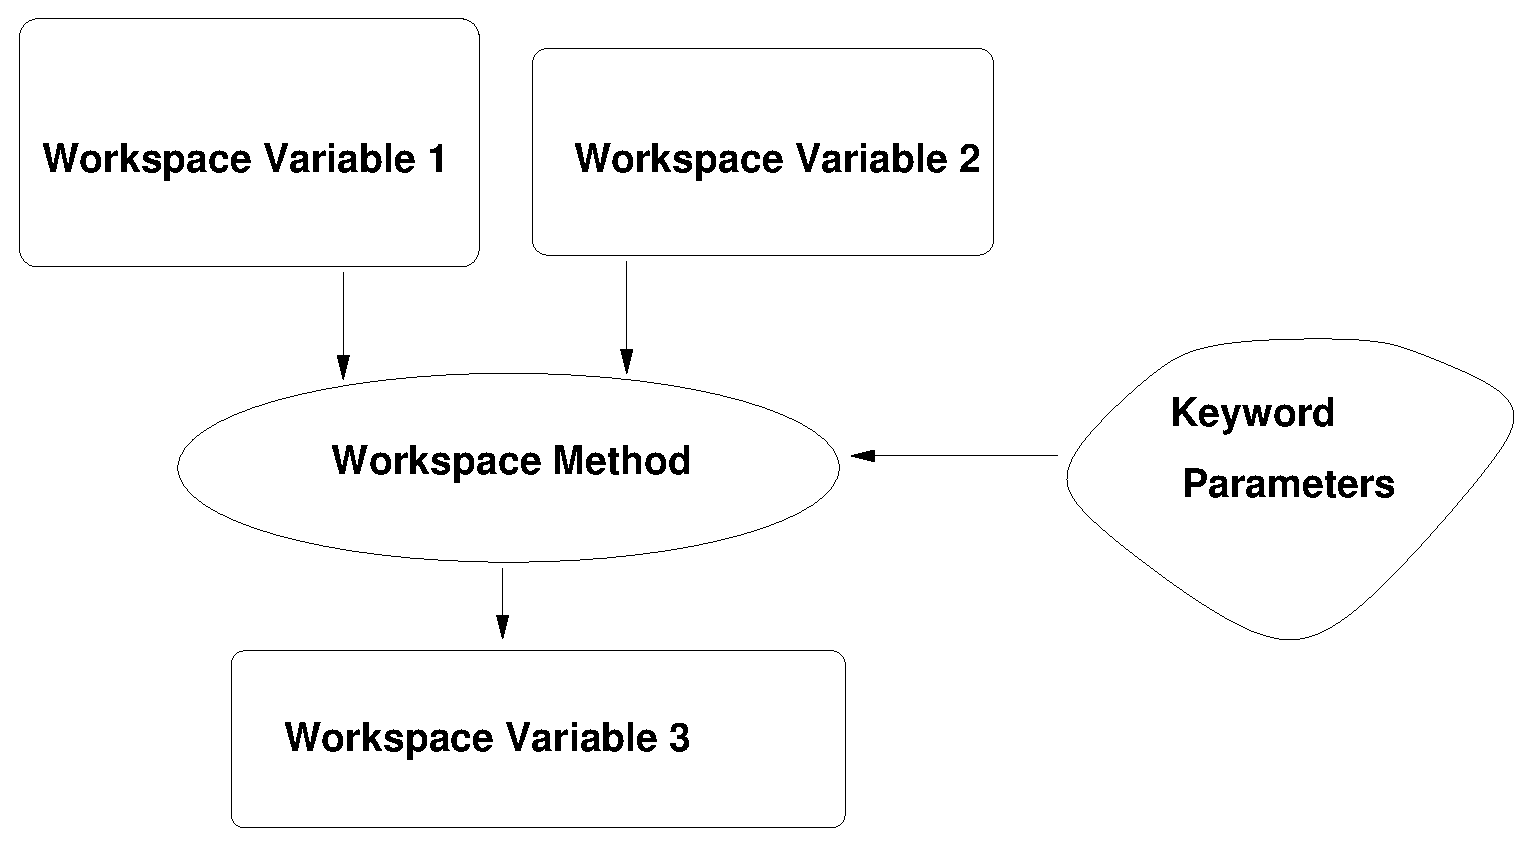
\includegraphics[width=\hsize,draft=false]{concept/method}
    \caption{\textindex{Specific
        workspace methods} act on specific workspace variables to
        generate other specific workspace variables. Additional input
        parameters can be specified as keyword parameters in the
        controlfile.}
    \label{fig:method}
  \end{center}
\end{figure}

It is important to note that the controlfile has a fixed and
well-defined syntax. This syntax is understood by the ARTS parser.
The great advantage of this concept is that it is very easy to add
new workspace variables and new workspace methods. The program has
an internal lookup table which lists all workspace methods, as well
as their input variables, output variables, and keyword
parameters. To add a new method, one just has to add an entry to
this lookup table, and write the code for the method itself. No
further changes to the program are necessary. In particular, no
changes to the program logic or to the parser. How such an extension
can be made practically is described in Section \ref{sec:development}.


\section{Generic Workspace Methods}
%=================================
\label{sec:concept:generic}

Generic methods (Figure \ref{fig:generic_method}) allow the user of
the program even more freedom than specific methods. A generic method
is for example \artsstyle{MatrixSet}, which can be used to set any
workspace variable which is a matrix. For example
\begin{quote}
  \artsstyle{MatrixSet(z\_surface){0.0}}
\end{quote}
will set all elements of \artsstyle{z\_surface} to 0.0 (as long as
\artsstyle{nrows} and \artsstyle{ncols} are set).

\begin{figure}
  \begin{center}
    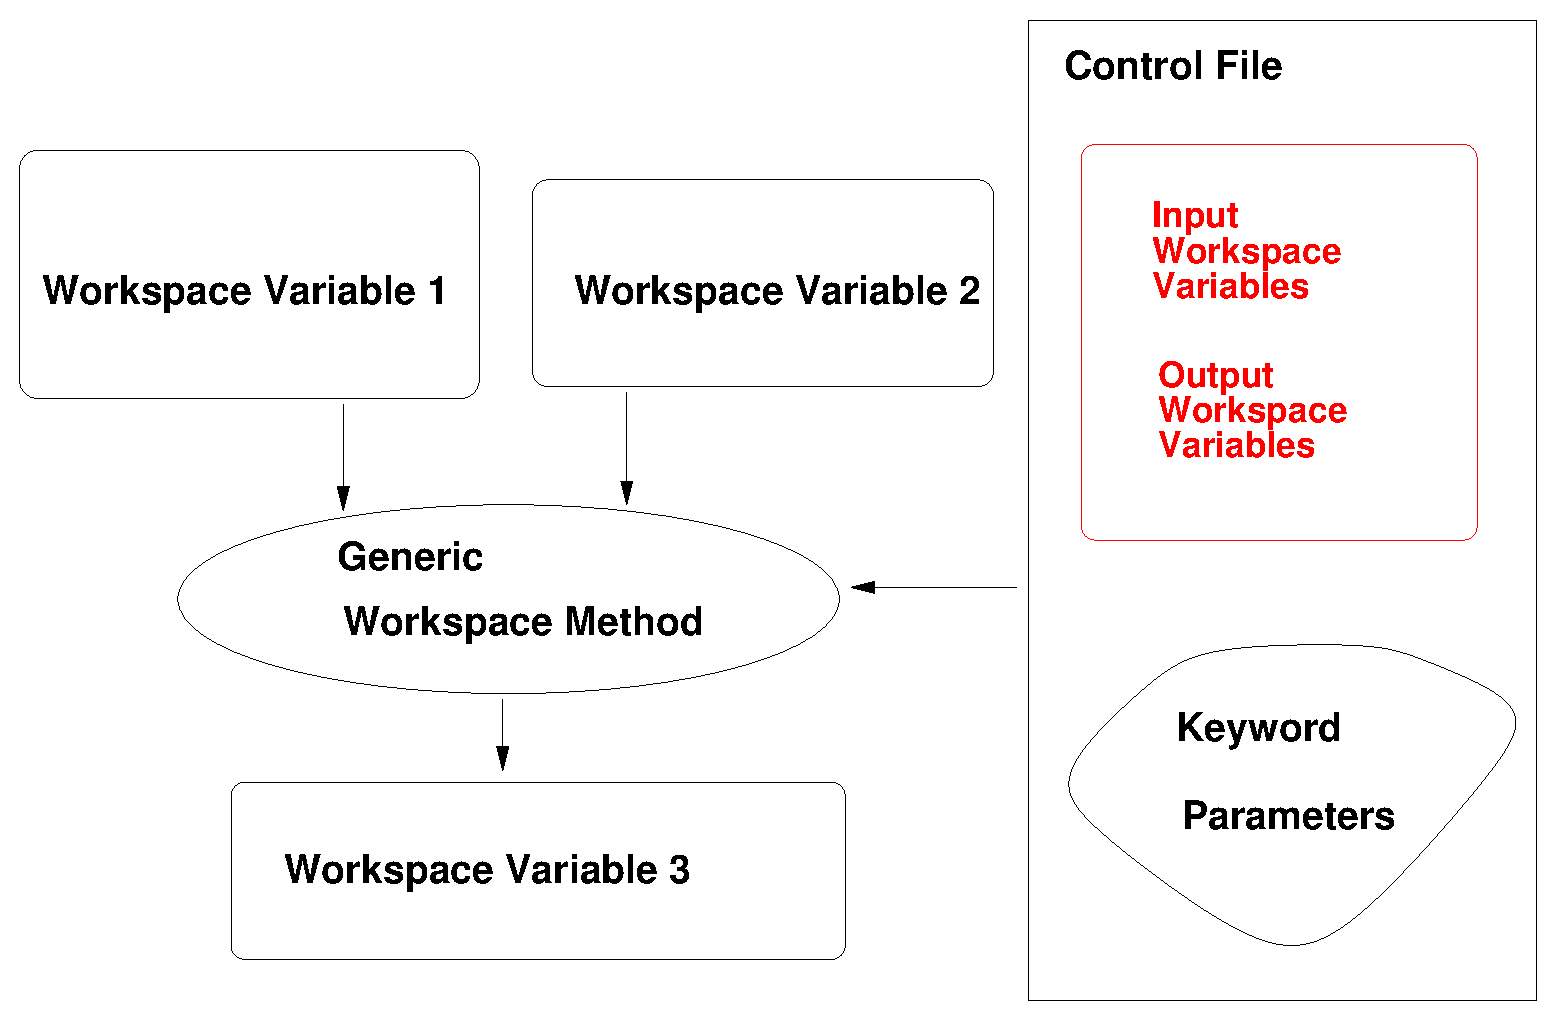
\includegraphics[width=\hsize,draft=false]{concept/generic_method}
    \caption{For \textindex{generic
      workspace methods} the workspace variables to act on are
        specified in the controlfile.}
    \label{fig:generic_method}
  \end{center}
\end{figure}

Some methods are even more flexible, the are super generic. This means
that they can take any workspace variable as input. The most commonly
used such methods are the XML file methods. A workspace variable is
read from a file in this way
\begin{quote}
  \artsstyle{ReadXML(f\_grid)\{"frequency\_grid"\}}
\end{quote}
Generic methods are particularly useful for IO operations like in the
example above. No new IO methods are necessary for new workspace
variables, as long as they are of standard types already known to the
program (for example vectors or matrices). 



\section{Agendas}
%=================================
\label{sec:concept:agendas}

Agendas are a special incarnation of a workspace method. In the
controlfile an arbitrary number of workspace methods can be added to
an agenda. On invocation, the agenda executes its methods one
after the other. The inputs and outputs defined for the agenda must
be satisfied by the invoked workspace methods. E.g., if an agenda
has \artsstyle{f\_grid} in its list of output workspace variables, a
workspace method which generates \artsstyle{f\_grid} must be added to
the agenda in the controlfile.

Even though it is possible to execute agendas directly from the
controlfile with the \artsstyle{AgendaExecute} method, the more common
and intended use case is the internal invocation by other workspace
methods. This adds a grave amount of flexibility to arts. The
\artsstyle{RteStd} method for example calculates (besides other
components) the emission term. Without the means of an agenda, it
would only be possible to use always the same method for the emission
calculation. By the use of an agenda the user can choose between
different methods to calculate the emission and plug them into the
emission agenda in the control file:

{\small
\begin{verbatim}
AgendaSet(emission_agenda){
  emissionPlanck{}
}
\end{verbatim}
}

\noindent
\artsstyle{RteStd} internally calls the \artsstyle{emission\_agenda} and
uses the user selected method for calculating the emission term.



\section{Practical hints}
%=================================
\label{sec:concept:practical}

The subdirectory \fileindex{tests} contains some example controlfiles.
You should study them to learn more about how the program works. You
can also run these controlfiles like this:
\begin{quote}
\begin{verbatim}
  arts simpleMC.arts
\end{verbatim}
\end{quote}
This assumes that you are inside the directory where the controlfiles
are, and that the \artsstyle{arts} executable is in your path.  You can
also run all of the examples, by saying
\begin{quote}
\begin{verbatim}
  make check
\end{verbatim}
\end{quote}

ARTS offers a number of useful command line parameters. In general,
there is a short form and a long form for each parameter. The short
form consists of a minus sign and a single letter, whereas the long
form consists of two minus signs and a descriptive name. To get a full
list, type
\begin{quote}
\begin{verbatim}
  arts -h
\end{verbatim}
\end{quote}
or
\begin{quote}
\begin{verbatim}
  arts --help
\end{verbatim}
\end{quote}
Most useful at the beginning should be the \artsstyle{-d}
(\artsstyle{--describe}), \artsstyle{-m} (\artsstyle{--methods}), \artsstyle{-w}
(\artsstyle{--workspacevariables}), and \artsstyle{-i} (\artsstyle{--input}) flags.
For instance, the \artsstyle{-d} (\artsstyle{--describe}) flag gives you online
documentation for any workspace method or workspace variable. Usage:
\begin{quote}
\begin{verbatim}
  arts -d f_grid
\end{verbatim}
\end{quote}
will print documentation about the workspace variable \artsstyle{f\_grid}, which
happens to be the monochromatic frequency grid.

But what methods and variables are available? You can find out by
typing
\begin{quote}
\begin{verbatim}
  arts -m all
\end{verbatim}
\end{quote}
which will list all workspace methods, or by typing 
\begin{quote}
\begin{verbatim}
  arts -w all
\end{verbatim}
\end{quote}
which will list all workspace variables. As you can see, these lists
are quite long. But you can get more specific information:
\begin{quote}
\begin{verbatim}
  arts -m f_grid
\end{verbatim}
\end{quote}
will give you a list of all methods that can generate the workspace
variable \artsstyle{f\_grid}. Specific and generic methods are listed
separately. Generic methods are in this case all methods producing a
Vector, since \artsstyle{f\_grid} belongs to this group. A similar task is
performed by the \artsstyle{-i} (\artsstyle{--input}) flag, with the difference
that \artsstyle{arts -i f\_grid} will list those methods that require
\artsstyle{f\_grid} as \emph{input}, whereas \artsstyle{arts -m f\_grid} lists
those that produce \artsstyle{f\_grid} as output. Finally,
\begin{quote}
\begin{verbatim}
  arts -w surfaceFlat
\end{verbatim}
\end{quote}
will give you all variables required by the method \artsstyle{abs\_coefCalc}
(the variable \artsstyle{f\_grid} happens to be one of them).

Using these command line parameters, it is easy to build up a
controlfile. The trick is, to start at the end. Say you want to
compute absorption coefficients. First of all, you have to find out
in which workspace variable these are stored. Look at the list
produced by \artsstyle{arts -w all}. You can use \artsstyle{arts -d} to look at
some candidates a bit more closely. This way, you will find out that
\artsstyle{abs\_coef} is the variable you are looking for.

In the next step, you can use \artsstyle{arts -m abs\_coef} to find all methods
that can calculate \artsstyle{abs\_coef}. So, you will find the method
\artsstyle{abs\_coefCalc}. Now you can use \artsstyle{arts -w abs\_coefCalc} to find out the
required input variables of that method. Then you can use the
\artsstyle{-m} flag again, to find the methods producing these variables,
and so on.

%%% Local Variables: 
%%% mode: latex
%%% TeX-master: "uguide"
%%% End: 

%
% To start the document, use
%  \levela{...}
% For lover level, sections use
%  \levelb{...}
%  \levelc{...}
%
\levela{Forward model concepts and definitions}
 \label{sec:fm_defs}

%
% Document history, format:
%  \starthistory
%    date1 & text .... \\
%    date2 & text .... \\
%    ....
%  \stophistory
%
\starthistory
  02xxxx & xxx.\\
\stophistory

This chapter introduces terms and concepts of ARTS as a forward model,
in contrast to the previous chapter that describes ARTS as a computer
programme. While the content of the previous chapter is specific for
ARTS, as the way to use a forward model programme differ normally
significantly from one implementation to another, this chapter is of
more general nature. Most of the quantities treated here should be
part of any forward model of the same complexity as ARTS, where only
details regarding the definition should differ. The aim of this chapter
is to describe important terms and concepts in such way that the 
content of this user guide can be fully appreciated and that you shall
understand how to generate a control file for your simulation problem. 




\levelb{Defining the atmosphere}
%===================
\label{sec:fm_defs:atmosphere}


 \begin{figure}
  \begin{center}
   \includegraphics*[width=0.95\hsize]{Figs/atm_dim_1d}
   \caption{ Schematic of a 1D atmosphere. The atmosphere is here circularly
     symmetric. This means that the radius of the geoid, the ground
     and all the pressure surfaces is constant. The cloud box extends
     from the ground up to the thin solid line. The upper limit of
     the cloud box coincides always with a pressure surface. }
   \label{fig:fm_defs:1d}  
  \end{center}
 \end{figure}
 % This figure was produced by the Matlab function mkfigs_atm_dims.

 \begin{figure}
  \begin{center}
   \includegraphics*[width=0.95\hsize]{Figs/atm_dim_2d}
   \caption{ Schematic of a 2D atmosphere. The radii of the geoid, the ground
     and all the pressure surfaces are for 2D atmospheres allowed to have a
     latitude variation. The limits of
     the cloud box coincide always with grid box boundaries. Plotting
     symbols as in Figure~\ref{fig:fm_defs:1d}. }
   \label{fig:fm_defs:2d}  
  \end{center}
 \end{figure}
 % This figure was produced by the Matlab function mkfigs_atm_dims.



%%% Local Variables: 
%%% mode: latex
%%% TeX-master: "uguide"
%%% End: 

%
\part{Algorithm Descriptions}
%
% To start the document, use
%  \levela{...}
% For lover level, sections use
%  \levelb{...}
%  \levelc{...}
%
\levela{Theoretical formalism}
 \label{sec:formalism}

%
% Document history, format:
%  \starthistory
%    date1 & text .... \\
%    date2 & text .... \\
%    ....
%  \stophistory
%
\starthistory
  000306 & Written by Patrick Eriksson, partly 
           based on \citet{eriksson:99} and \citet{eriksson:00a}. \\
\stophistory



%
% Symbol table, format:
%  \startsymbols
%    ... & \verb|...| & text ... \\
%    ... & \verb|...| & text ... \\
%    ....
%  \stopsymbols
%
%
%\startsymbols
%  \mpbi   & \verb|y|      & monochromatic pencil beam intensity      \\
%  \f      & \verb|f_mono| & monochromatic frequency                  \\
%  \view   & \verb|za_pencil| & pencil beam zenith angle              \\
%  \iv     & \verb|y|      & vector of monochromatic pencil beam intensities \\
%  \y      & \verb|y|      & spectrum recorded by a sensor            \\
%  \fm     & \verb|-|      & forward model                            \\
%  \fma    & \verb|-|      & atmospheric part of \fm                  \\
%  \fms    & \verb|-|      & sensor part of \fm                       \\
%  \xt     & \verb|-|      & state vector (variables to be retrieved) \\
%  $\xt_r$ & \verb|-|      & atmospheric part of \xt                  \\
%  $\xt_s$ & \verb|-|      & sensor part of \xt                       \\
%  $\xt_\merr$& \verb|-|   & part of \xt\ describing measurement errors   \\
%  \bt     & \verb|-|      & forward model parameter vector           \\
%  $\bt_r$ & \verb|-|      & atmospheric part of \bt                  \\
%  $\bt_s$ & \verb|-|      & sensor part of \bt                       \\
%  $\bt_\merr$& \verb|-|   & part of \bt\ describing measurement errors   \\
%  \Kx     & \verb|k|      & state weighting function matrix          \\
%  \Kb     & \verb|k|      & model parameter weighting function matrix\\  
% \label{symtable:formalism}     
%\stopsymbols



%
% Introduction
%
In this section a theoretical framework for the forward model is
presented. The presentation follows \citet{rodgers:90}, but some
extensions are made, for example, the distinction between the
atmospheric and sensor parts of the forward model is also discussed
here.



\levelb{The forward model}
 \label{sec:formalism:fm}
 
 The radiative intensity, \mpbi, at a point in the atmosphere, $r$, for
 frequency \f\ and traversing in the direction, \view, is dependent
 on a variety of physical processes and continuous variables such as
 the temperature profile, $T$:

 \begin{equation}
   \mpbi = F(r,\f,\view,T,\dots)
 \end{equation} 
 To detect the spectral radiation some kind of sensor, having a finite
 spatial and frequency resolution, is needed, and the observed
 spectrum becomes a vector, \y, instead of a continuous function.
 The atmospheric radiative transfer is simulated by a computer model
 using a limited number of parameters as input, and the forward model,
 \fm, used in practice can be expressed as
 
 \begin{equation}
   \y = \fm(\xt_\fm,\bt_\fm) + \merr(\xt_\merr,\bt_\merr)
  \label{eq:formalism:fm}
 \end{equation}
 where $(\xt_\fm,\bt_\fm)$ and $(\xt_\merr,\bt_\merr)$ together give a
 total description of both the atmospheric and sensor states, and
 \merr\ is the measurement errors. The parameters are divided in such
 way that \xt, the state vector, contains the parameters to be
 retrieved, and the remainder is given by \bt, the model parameter
 vector. The total state vector is
 \begin{equation}
   \xt = \left[ \begin{array}{c} \xt_\fm \\ \xt_\merr \end{array} \right]
 \end{equation}
 and the total model parameter vector is
 \begin{equation}
   \bt = \left[ \begin{array}{c} \bt_\fm \\ \bt_\merr \end{array} \right]
 \end{equation}
 The actual forward model consists of either empirically determined
 relationships, or numerical counterparts of the physical
 relationships needed to describe the radiative transfer and sensor
 effects. The forward model described here is mainly of the latter
 type, but some parts are more based on empirical investigations, such
 as the parameterisations of continuum absorption. It should be noted
 that a possible data reduction is also part of the forward model.
  
 Both for the theoretical formalism and the practical implementation,
 it is suitable to make a separation of the forward model into two
 main sections, a first part describing the atmospheric radiative
 transfer for pencil beam (infinite spatial resolution) monochromatic
 (infinite frequency resolution) signals \citep{eriksson:99},

 \begin{equation}
   \iv = \fma(\xt_r,\bt_r)
  \label{eq:formalism:fma}
 \end{equation}
 and a second part modelling sensor characteristics,
 \begin{equation}
   \y = \fms(\iv,\xt_s,\bt_s) + \merr(\xt_\merr,\bt_\merr)
  \label{eq:formalism:fms}
 \end{equation}
 where \iv\ is the vector holding the spectral values for the
 considered set of frequencies and viewing angles (i.e.
 $\iv^i=I(\f^i,\view^i)$, where $i$ is the vector index), and
 $\xt_\fm$ and $\bt_\fm$ are separated correspondingly, that is,
 $\xt_\fm^T= [\xt_r^T,\xt_s^T]$ and $\bt_\fm^T= [\bt_r^T,\bt_s^T]$. The
 vectors \xt\ and \bt\ can now be expressed as
 \begin{equation}
   \xt = \left[ \begin{array}{c} \xt_r\\ \xt_s \\ \xt_\merr \end{array} \right]
 \end{equation}
 and
 \begin{equation}
   \bt = \left[ \begin{array}{c} \bt_r\\ \bt_s \\ \bt_\merr \end{array}\right],
 \end{equation}
 respectively.

 The subscripts of \xt\ and \bt\ are below omitted if the part of the
 vectors used is made clear by the context. 



\levelb{The sensor transfer matrix} 
 \label{sec:formalism:sensor}
  
 The modelling of the different sensor parts can be described by a
 number of of analytical expressions (see \citet{eriksson:97a}) that
 together makes the basis for the sensor model. These expressions are
 throughout linear operations and it possible, as suggested in
 \citet{eriksson:00a}, to implement the sensor model as a
 straightforward matrix multiplication:
 \begin{equation}
   \y = \Hm \iv + \merr
  \label{eq:formalism:H}
 \end{equation}
 where \Hm\ is here denoted as the sensor transfer matrix.  The matrix
 \Hm\ can  be set up to incorporate effects of a data reduction and
 the total transfer matrix is then
 \begin{equation}
   \Hm = \Hd \Hs
  \label{eq:formalism:Hs}
 \end{equation}
 as
 \begin{equation}
   \y = \Hd \y' = \Hd (\Hs \iv + \merr') = \Hm \iv + \merr
  \label{eq:formalism:datared}
 \end{equation}
 where \Hd\ is the reduction matrix, \Hs\ the sensor matrix, and $\y'$
 and $\merr'$ are the measurement vector and the measurement errors,
 respectively, before data reduction. The matrices \Hd\ and \Hs\ are
 described in Section \ref{sec:sensor} and \ref{sec:red}, respectively.



\levelb{Weighting functions} 
 \label{sec:formalism:wfuns}

 \levelc{Basics} 
 A weighting function is the partial derivative of the spectrum vector
 \y\ with respect to some variable used by the forward model.  As the
 input of the forward model is divided between \xt\ or \bt, the
 weighting functions are divided correspondingly between two matrices,
 the state weighting function matrix

 \begin{equation}
   \Kx = \frac{\partial \y}{\partial \xt}
  \label{eq:formalism:kx}
 \end{equation}
 and the model parameter weighting function matrix
 \begin{equation}
   \Kb = \frac{\partial \y}{\partial \bt}
  \label{eq:formalism:kb}
 \end{equation}
 For the practical calculations of the weighting functions, it is
 important to note that the atmospheric and sensor parts can be
 seperated. For example, if \xt\ only hold atmospheric and
 spectroscopic variables, \Kx\ can be expressed as

 \begin{equation}
   \Kx = \frac{\partial \y}{\partial \iv}\frac{\partial\iv}{\partial \xt} =
    \Hm\frac{\partial\iv}{\partial \xt}
  \label{eq:formalism:kx2}
 \end{equation}
 This equation shows that the new parts needed to calculate
 atmospheric weighting functions, are functions giving $\partial\iv /
 \partial \xt$ where \xt\ can represent the vertical profile of a
 species, atmospheric temperature, spectroscopic data etc.
 
 The practical calculation of weighting functions is discussed in
 detail in Sections \ref{sec:wfuns} and \ref{sec:wfuns_sens}.


 \levelc{Transformation between vector spaces}
 
  It could be of interest to transform a weighting function matrix from
  one vector space to another. The new vector, $\xt'$, is here
  assumed to be of length $n$ $(\xt' \in \msize{n}{1})$, while the original
  vector, \xt\ is of length $p$ $(\xt \in \msize{p}{1})$.  The
  relationship between the two vector spaces is described by a
  transformation matrix $\B$:
  \begin{equation}
    \xt = \B\xt'
  \end{equation}
  where $\B \in \msize{p}{n}$. For example, if $\xt'$ is assumed to be
  piecewise linear, then the columns of $\B$ contain tenth functions,
  that is, a function that are 1 at the point of interest and decreases
  linearly down to zero at the neighbouring points.  The matrix can
  also hold a reduced set of eigenvectors.
    
  The weighting function matrix corresponding to $\xt'$ is
  \begin{equation}
    \K_{\xt'} = \frac{\partial \y}{\partial \xt'}
  \end{equation}
  This matrix is related to the weighting function matrix of \xt\ (Eq.
  \ref{eq:formalism:kx}) as
  \begin{equation}
    \K_{\xt'}
      = \frac{\partial \y}{\partial \xt} \frac{\partial \xt}{\partial \xt'}
      = \frac{\partial \y}{\partial \xt} \B 
      = \Kx \B
  \end{equation}
  Note that
  \begin{equation}
    \K_{\xt'}\xt' = \Kx\B\xt' =  \Kx\xt
  \end{equation}
  However, it should be noted that this relationship only holds for
  those \xt\ that can be represented perfectly by some $\xt'$ (or vice
  versa), that is, $\xt=\B\xt'$, and not for all combinations of \xt\ 
  and $\xt'$.

  If $\xt'$ is the vector to be retrieved, we have that \citep{rodgers:90}
  \begin{equation}
    \xret' = \im(\y,\ct) = \tm(\xt,\bt,\ct)
  \end{equation}
  where \im\ and \tm\ are the inverse and transfer model, respectively.

  The contribution function matrix is accordingly
  \begin{equation}
    \Dy =  \frac{\partial \xret'}{\partial \y}
  \end{equation}
  that is, \Dy\ corresponds to $\K_{\xt'}$, not \Kx.
  
  We have now two possible averaging kernel matrices
  \begin{equation}
    \A_{\xt} 
      = \frac{\partial \xret'}{\partial \xt} 
      = \frac{\partial \xret'}{\partial \y} \frac{\partial \y}{\partial \xt}
      = \Dy \Kx
  \end{equation}
  \begin{equation}
    \A_{\xt'} 
      = \frac{\partial \xret'}{\partial \xt'} 
      = \frac{\partial\xret'}{\partial\y}\frac{\partial\y}{\partial\xt}
      \frac{\partial\xt}{\partial\xt'}
      = \Dy \K_{\xt'}
      = \A_{\xt} \B
  \end{equation}
  where $\A_{\xt} \in \msize{p}{n}$ and $\A_{\xt'} \in
  \msize{p}{p}$, that is, only $\A_{\xt'}$ is square. 




%%% Local Variables: 
%%% mode: latex
%%% TeX-master: "uguide"
%%% End: 

%
% To start the document, use
%  \levela{...}
% For lover level, sections use
%  \levelb{...}
%  \levelc{...}
%
\levela{Gas Absorption}
 \label{sec:absorption}


%
% Document history, format:
%  \starthistory
%    date1 & text .... \\
%    date2 & text .... \\
%    ....
%  \stophistory
%
\starthistory
  2001-07-05 & Template created by Stefan Buehler.\\
\stophistory


%
% Symbol table, format:
%  \startsymbols
%    ... & \verb|...| & text ... \\
%    ... & \verb|...| & text ... \\
%    ....
%  \stopsymbols
%
%
%\startsymbols
%  -- & -- & -- \\
% \label{symtable:wfuns}     
%\stopsymbols


Some general introduction here, also explaining the structure of this chapter.



\levelb{Line Absorption}
%-----------------------
\label{sec:line_absorption}

Some introduction here, how line by line absorption is calculated in
principle. (Should define intensity, partition function, line shape, etc.)

\levelc{Line Catalogues} 

Mostly describe the ARTS internal format, but also briefly list the
other catalogues that can be read by ARTS

\levelc{Species specific data} 

Molecular mass, etc. 

\levelc{Partition Functions}

These are strictly also species specific data, but they seem to deserve
their own section.

\levelc{Line Shape Functions}


\levelc{ARTS Workspace Variables and Methods}



\levelb{Continua and Complete Absorption Models}
%-----------------------------------------------

There should be some general introduction here.

The headings here are tentative, TBD by Thomas.

\levelc{H2O Models}

\levelc{Dry air Models}

\levelc{ARTS Workspace Variables and Methods}


 



%%% Local Variables: 
%%% mode: latex 
%%% TeX-master: "uguide" 
%%% End:


\chapter{Propagation paths}
 \label{sec:ppath}


\starthistory
  120202 & Revised and parts moved to \theory\ (Patrick Eriksson).\\
  030310 & First complete version written by Patrick Eriksson.\\
\stophistory


\graphicspath{{Figs/ppath/}}


A propagation path is the name given in ARTS to the way the radiation travels
to reach the sensor for a specified line-of-sight. Propagation paths are
introduced in Section \ref{sec:fm_defs:ppaths} and this section provides
further details. For a general usage of ARTS, it should suffice to read
Section~\ref{sec:ppath:usage}. The remaining sub-sections deal with more
low-level aspects of the calculations, and are of interest only if you want to
understand the finer details of ARTS. The actual equations used are found in
Chapter~\ref{T-sec:ppaththeory} of \theory.



\section{Practical usage}
%===================
\label{sec:ppath:usage}

The ray tracing algorithm to be applied for the calculation of propagation path
is effectively selected by specifying \wsaindex{ppath\_step\_agenda} (see
further Section~\ref{sec:fm_defs:ppaths}). The fastest calculations are
obtained if refraction is neglected, denoted as geometrical calcutions. The
workspace method to apply if this assumption can be made is
\wsmindex{ppath\_stepGeometric}.

The main consideration for using \builtindoc{ppath\_stepGeometric} is to select
a value for \wsvindex{ppath\_lmax}. This variable controls to some extent the
calculation accuarcy, as described in Section~\ref{sec:fm_defs:accuracy}. This
variable sets the maximum distance between points of the (final) propagation
path. Set this variable to e.g.\ -1 if you don't want to apply such a length
criterion.

A straightforward, but inefficient, treatment of refraction is provided by
\wsmindex{ppath\_stepRefractionEuler}. This method divides the propagation path
into a series of geomtrical ray tracing steps. The size of the ray tracing
steps is selected by \wsvindex{ppath\_lraytrace}. This variable affects only
the ray tracing part, the distance between points of the propagation path
actually returned is controled by \builtindoc{ppath\_lmax} as above.





\section{Calculation approach}
%===================
\label{sec:ppath:approach}

The propagation paths are calculated in steps, as outlined in
Section~\ref{sec:fm_defs:ppaths}. The path steps are normally from one crossing
of the atmospheric grids to next. To introduce
propagation paths steps was necessary to handle the iterative solution for
scattering inside the cloud box, as made clear from Figure
\ref{fig:scattering:average}.

A full propagation path is stored in the workspace variable \wsvindex{ppath},
that is of the type \builtindoc{Ppath} (see Section \ref{sec:ppath:Ppath}). The
paths are determined by calculating a number of path steps. A path step is the
path from a point to the next crossing of either the pressure, latitude or
longitude grid (Figure~\ref{fig:ppath:ex1}). There is one
exception to this definition of a path step, and that is when there is an
intersection with the surface, which ends the propagation path at that point.
The starting point for the calculation of a path step is normally a grid
crossing point, but can also be an arbitrary point inside the atmosphere, such
as the sensor position. Only points inside the model atmosphere are handled.
The path steps are stored in the workspace variable \wsvindex{ppath\_step},
that is of the same type as \builtindoc{ppath}.

\begin{figure}
 \begin{center}
  \includegraphics*[width=0.80\hsize]{ppath_ex1}
  \caption{Tracking of propagation paths. For legend, see 
    Figure \ref{fig:ppath:ex2}. The figure tries to visualize how the
    calculations of propagation paths are performed from one grid cell
    to next. In this example, the calculations start directly at the
    sensor position $(\ast)$ as it placed inside the model
    atmosphere. The circles give the points defining the propagation
    path. Path points are always included at the crossings of the grid
    cell boundaries. Such a point is then used as the starting point
    for the calculations inside the next grid cell. }
  \label{fig:ppath:ex1}  
 \end{center}
\end{figure}
% This figure was produced by the Matlab function mkfigs_ppath

\begin{figure}
 \begin{center}
   \includegraphics*[width=0.98\hsize]{ppath_ex2}
  \caption{As Figure \ref{fig:ppath:ex1}, but with a length criterion 
    for the distance between the points defining the path.
    The inclusion of the tangent point is not a result of this length
    criterion, it is always included among the path points.}
  \label{fig:ppath:ex2}  
 \end{center}
\end{figure}
% This figure was produced by the Matlab function mkfigs_ppath


Propagation paths are calculated with the internal function
\funcindex{ppath\_calc}. The communication between this method and
\builtindoc{ppath\_step\_agenda} is handled by \builtindoc{ppath\_step}.
That variable is used both as input and output to
\builtindoc{ppath\_step\_agenda}.  The agenda gets back
\builtindoc{ppath\_step} as returned to \builtindoc{ppath\_calc} and the
last path point hold by the structure is accordingly the starting
point for the new calculations. If a total propagation path shall be
determined, the agenda is called repeatedly until the starting point
of the propagation path is found and \builtindoc{ppath\_step} will hold
all path steps that together make up \builtindoc{ppath}. The starting
point is included in the returned structure.

The path is determined by starting at the end point and moving
backwards to the starting point. The calculations are initiated by
filling \builtindoc{ppath\_step} with the practical end point of the
path. This is either the position of the sensor (true or
hypothetical), or some point at the top of the atmosphere (determined
by geometrical calculations starting at the sensor). This
initialization is not handled by \builtindoc{ppath\_step\_agenda}. 
The field \shortcode{constant} is set by \builtindoc{ppath\_calc}
to the correct value if the sensor is above the model atmosphere.
Otherwise, the field is set to be negative and is corrected by
\builtindoc{ppath\_step\_agenda} at the first call. This procedure is
needed as the propagation path constant changes if refraction is
considered, or not, when the sensor is placed inside the atmosphere.

The agenda performs only calculations to next crossing of a grid, all
other tasks are performed by \builtindoc{ppath\_calc}, with one exception.
If there is an intersection with the surface, the calculations stop at
this point. This is flagged by setting the background field of
\builtindoc{ppath\_step}. Beside this, \builtindoc{ppath\_calc} checks if
the starting point of the calculations is inside the scattering box or
below the surface level, and check if the last point of the path has
been reached. 

In many cases the propagation path can/must be considered to consist
of several parts. One exemple is surface reflection (see
Figure \ref{fig:fm_defs:surface_refl}). The variable \builtindoc{ppath}
describes then only a single part of the propagation path.



\section{The propagation path data structure}
%===================
\label{sec:ppath:Ppath}

A propagation path is represented by a structure of type
\typeindex{Ppath}. This structure holds also auxiliary variables to
facilitate the radiative transfer calculations and to speed up the
interpolation. The fields of \builtindoc{Ppath} are described below,
where the data type is given inside square brackets. 

\begin{description}

  \item[dim] [Index] The atmospheric dimensionality. This field shall always 
     be equal to the workspace variable \builtindoc{atmosphere\_dim}.
     
   \item[np] [Index] Number of positions to define the propagation
     path. Allowed values are $\geq 0$. The number of rows of
     \shortcode{pos} and \shortcode{los}, and the length of
     \shortcode{z}, \shortcode{gp\_p}, \shortcode{gp\_lat} and
     \shortcode{gp\_lon}, shall be equal to \shortcode{np}. The length
     of \shortcode{l\_step} is \shortcode{np} - 1. If \shortcode{np}
     $\leq$ 1, the observed spectrum is identical to the radiative
     background. For cases where the sensor is placed inside the model
     atmosphere and \shortcode{np} = 1, the stored position is
     identical to the sensor position and that position can be used to
     determinate the radiative background (see below).

   \item[constant] [Numeric] The propagation path constant. Such a
     constant can be assigned to all geometrical paths and for 1D
     cases (with or without refraction). This field can be
     initiated to a negative value to indicate that the constant is
     undefined or not yet set. For cases where the constant applies,
     \builtindoc{ppath\_step\_agenda} sets this constant at the first
     call of the agenda if the given value is negative.

   \item[pos] [Matrix] The position of the propagation path points.
     This matrix has \shortcode{np} rows and up to 3 columns. Each row
     holds a position where column 1 is the radius, column 2 the
     latitude and column 3 the longitude (cf.
     Section \ref{sec:fm_defs:sensorpos}). The number of columns for
     1D and 2D is 2, while for 3D it is 3. The latitudes are stored
     for 1D cases as these can be of interest for some applications
     and are useful if the propagation path shall be plotted. The
     latitudes for 1D give the angular distance to the sensor (see
     further Section \ref{sec:fm_defs:atmdim}).
     The propagation path is stored in reversed order, that is, the
     position with index 0 is the path point closest to the sensor
     (and equals the sensor position if it is inside the atmosphere).
     The full path is stored also for 1D cases with symmetry around a
     tangent point (in contrast to ARTS-1). 
     
  \item[z] [Vector] The geometrical altitude for each path position. The
     length of this vector is accordingly \shortcode{np}. This is a help
     variable for plotting and similar purposes. It shall not be used to
     interpolate the atmospheric fields, as pressure is the main altitude
     coordinate.
     
   \item[l\_step] [Vector] The length along the propagation path
     between the positions in \shortcode{pos}. The first value is the
     length between the first and second point etc. For \shortcode{np}
     $\geq 2$, the length of the vector is \shortcode{np} - 1.
     Otherwise it is 0.

   \item[gp\_p] [ArrayOfGridPos] Index position with respect to the
     pressure grid. The structure for grid positions is described in
     \developer, Section \ref{D-sec:interpolation:gridpos}. 
     
   \item[gp\_lat] [ArrayOfGridPos] As \shortcode{gp\_p} but with
     respect to the latitude grid.

   \item[gp\_lon] [ArrayOfGridPos] As \shortcode{gp\_p} but with
     respect to the longitude grid.
     
   \item[los] [Matrix] The line-of-sight of the propagation path at
     each point. The number of rows of the matrix is \shortcode{np}.
     For 1D and 2D, the matrix has a single column holding the zenith
     angle. For 3D there is an additional column giving the azimuth
     angle. The zenith and azimuth angles are defined in
     Section \ref{sec:fm_defs:los}. If the radiative background is the
     cloud box, the last position (in \shortcode{pos}) and
     line-of-sight give the relevant information needed when
     extracting the radiative background from the cloud box intensity
     field.
     
   \item[background] [String] The radiative background for the
     propagation path. The possible
     options for this field are 'space', 'blackbody surface', 'cloud
     box interior' and 'cloud box surface', where the source of
     radiation should be clear the content of the strings.
     
   \item[tan\_pos] [Vector] The position of the tangent point. This
     vector is only set if there exists a tangent point (above the
     surface level), the length of the vector is otherwise 0. The
     tangent point is defined as the point with the lowest radius
     along the path. This means that (the absolute value of) the
     zenith angle at the tangent point is always 90\degree. For 2D
     and 3D this point can deviate from the point with lowest
     geometrical altitude.
     
   \item[geom\_tan\_pos] [Vector] The position of the geometrical
     tangent point. This vector is set for all downward observations.
     Refraction and surface reflections are neglected when calculating
     this tangent point position. This field is not handled by
     \builtindoc{ppath\_step\_agenda}. Definition of the tangent point
     as for \shortcode{tan\_pos}.

   \item[nreal] [Vector] The real part of the refractive index at each path
     position. Length is accordingly \shortcode{np}. 

\end{description}




\section{Structure of implementation}
%===================
\label{sec:ppath:structure}

The workspace method for calculating propagation paths is
\wsmindex{ppathCalc}, but this is just a getaway function for
\builtindoc{ppath\_calc}. The main use of \builtindoc{ppathCalc} is to
debug and test the path calculations, and that WSM should normally not
be part of the control file. Propagation paths, or steps, are
generated from inside other functions.


\subsection{Main functions for clear sky paths}
%===================

The master function to calculate full clear sky propagation paths is
\funcindex{ppath\_calc}. This function is outlined in
Algorithm \ref{alg:ppath:ppath_calc}. The function can be divided into
three main parts, initialization (handled by
\builtindoc{ppath\_start\_stepping}), a repeated call of
\builtindoc{ppath\_step\_agenda} and putting data into the return
structure (\builtindoc{ppath}).

\begin{algorithm}
 \begin{algorithmic}
  \STATE{check consistency of function input}
  \STATE{call \builtindoc{ppath\_start\_stepping} to set 
    \builtindoc{ppath\_step}}
  \STATE{create an array of \builtindoc{Ppath} structures, 
         \builtindoc{ppath\_array}}
  \STATE{add \builtindoc{ppath\_step} to \builtindoc{ppath\_array}}
  \WHILE{radiative background not reached}
   \STATE{call \wsaindex{ppath\_step\_agenda}}
   \IF{path is at the highest pressure surface}
    \STATE{radiative background is space}
   \ELSIF{path is at either end point of latitude or longitude grid}
    \STATE{this is not allowed, issue an runtime error}
   \ENDIF
   \IF{cloud box is active}
    \IF{path is at the surface of the cloud box}
     \STATE{radiative background is the cloud box surface}
    \ENDIF
   \ENDIF
   \STATE{add \builtindoc{ppath\_step} to \builtindoc{ppath\_array}}
  \ENDWHILE
  \STATE{initialize the WSV \builtindoc{ppath} to hold found number of 
         path points} 
  \STATE{copy data from \builtindoc{ppath\_array} to \builtindoc{ppath}}
 \end{algorithmic}
 \caption{Outline of the function \builtindoc{ppath\_calc}.}
 \label{alg:ppath:ppath_calc}
\end{algorithm}

The main task of the function \funcindex{ppath\_start\_stepping} is to
set up \wsvindex{ppath\_step} for the first call of
\builtindoc{ppath\_step\_agenda}, which means that the practical
starting point for the path calculations must be determined. If the
sensor is placed inside the model atmosphere, the sensor position
gives directly the starting point. For cases when the sensor is found
outside the atmosphere, the point where the path exits the atmosphere
must be determined. The exit point can be determined by pure
geometrical calculations (see Sections \ref{sec:ppath:basicgeom} and
\ref{sec:ppath:stepcalc}) as the refractive index is assumed to have the
constant value of 1 outside the atmosphere. The problem is accordingly
to find the geometrical crossing between the limit of the atmosphere
and the sensor line-of-sight (LOS). The function performs further some
other tasks, which include:
\begin{itemize}
\item For all LOS with a zenith angle $\geq 90\degree$ the position of
  the geometrical tangent point is calculated.
\item If the sensor is placed inside the model atmosphere
  \begin{itemize}
  \item Checks that the sensor is placed above the surface level. If
    not, an error is issued.
  \item Checks for 2D and 3D and when the sensor position as at an end
    point of the latitude or longitude grid, that the LOS is inwards
    with respect to the atmospheric limit.
  \item If the sensor and surface altitudes are equal, and the sensor
    LOS is downward, the radiative background is set to be the
    surface. For 2D and 3D, the tilt of the surface radius is considered
    when determining if the LOS is downward.
  \item If the cloud box is active and the sensor position is inside
    the cloud box, the radiative backsurface is set to be ``cloud box
    interior''. All sensor positions on the cloud box surface are for
    2D and 3D treated as points inside the box (for simplicity
    reasons), while for 1D the behavior is as expected.
  \end{itemize}
\item If the sensor is placed outside the model atmosphere
  \begin{itemize}
  \item Checks that the zenith angle is $\geq  90\degree$.  Upward
    observations are here not allowed.
  \item If it is found for 2D and 3D that the exit point of the path
    not is at the top of the atmosphere, but is either at a latitude
    or longitude end face of the atmosphere, an error is issued. This
    problem can not appear for 1D.
  \end{itemize}
\end{itemize}
For further details, see the code.


\subsection{Main functions for propagation path steps}
%===================

Example on workspace methods to calculate propagation path steps are
\wsmindex{ppath\_stepGeometric} and
\wsmindex{ppath\_stepRefractionEuler}. All such methods adapt
automatically to the atmospheric dimensionality, but the different
dimensionalities are handled by separate internal functions. For
example, the sub-functions to \builtindoc{ppath\_stepGeometric} are
\funcindex{ppath\_step\_geom\_1d}, \funcindex{ppath\_step\_geom\_2d}
and \funcindex{ppath\_step\_geom\_3d}. See \shortcode{m\_ppath.cc} to
get the names of the sub-functions for other propagation path step
workspace methods. 

\begin{algorithm}
 \begin{algorithmic}
  \STATE{call \funcindex{ppath\_start\_2d}}
  \IF{\shortcode{ppath\_step.ppc} $<1$}
   \STATE{calculate the path constant}
   \COMMENT{this is then first path step}
  \ENDIF
  \STATE{call \funcindex{do\_gridcell\_2d}}
  \STATE{call \funcindex{ppath\_end\_2d}}
  \IF{calculated step ends with tangent point}
   \STATE{call \shortcode{ppath\_step\_geom\_2d} with temporary 
     \shortcode{Ppath} structure}
   \STATE{append temporary \shortcode{Ppath} structure to 
     \shortcode{ppath\_step}}
  \ENDIF
 \end{algorithmic}
 \caption{Outline of the function \funcindex{ppath\_step\_geom\_2d}.}
 \label{alg:ppath:ppath_step_geom_2d}
\end{algorithm}

Many tasks are independent of the algorithm for refraction that is
used, or if refraction is considered at all. These tasks are solved by
two functions for each atmospheric dimensionality. For 1D the
functions are \funcindex{ppath\_start\_1d} and
\funcindex{ppath\_end\_1d}, and the corresponding functions for 2D and
3D are named in the same way. The functions to calculate geometrical
path steps are denoted as \funcindex{do\_gridrange\_1d},
\funcindex{do\_gridcell\_2d} and \funcindex{do\_gridcell\_3d}. Paths
steps passing a tangent point are handled by a recursive call of the
step function. Algorithm \ref{alg:ppath:ppath_step_geom_2d} summerizes
this for geometrical 2D steps.


\section{General comments}
%===================
\label{sec:ppath:comments}

The calculation of propagation paths involves a number of mathematical
expressions and they are presented in
Sections \ref{sec:ppath:basicgeom}--\ref{sec:ppath:refreuler}. In
addition, the path calculations present a number of practical
problems. These practical problems are discussed briefly in this
section. For further details, see the code.


\subsection{Numerical precision}
%===================

The aim here is not to make a complete discussion around the limited
numerical accuracy, but just to point out some of the problems caused.
We can start by noticing that the precision with which atmospheric
positions can be given is about 0.5\,m when the numeric type is
\textindex{float} and 2\topowerten{-8}\,m for \textindex{double}
(assuming that the mantissa has 24 and 48 bits, respectively). The
numbers given correspond to the change of the position for a change of
1 bit, in either radius, latitude and longitude. Already these numbers
cause problems for the approach taken to calculate propagation paths.
For any path along the border of a grid cell, any rounding error in
the wrong direction will move the position outside the grid cell,
which would lead to a crash of the code without countermeasures.

The values above give the representation precision. The precision will
be even poorer if a position is obtained by calculations as numerical
problems tend to accumulate. The calculation precision depends on what
mathematical expressions that are involved.  For example, a radius or
length obtained by the Pythagorean relation will have a relatively
high uncertainty as the calculations involve taking the square of a
radius in the order of 6400\,km. It was found that for calculations
performed using only float as numeric type, could lead to
displacements from the true position up to 10\,m. It was first tried to
hard-code double as the numerical type for the most critical passages
of the calculations, but a total success was not achieved and some
code had to be duplicated (to be used with either the float or double
option by if-statements for the pre-compiler) to avoid compiler
warnings. A step further was then taken, and double is now hard-coded
for all internal variables of \fileindex{ppath.cc}. This deviation
from the rule to have an uniform numeric type inside ARTS was
introduced to avoid more complicated coding and it has a very small
impact on the overall calculation speed. However, this measure will
not lead to that the precision of the path calculations will be the
same for float and double, as the results will be converted to float
between each propagation path step when copied to
\builtindoc{ppath\_step}.

As pointed out above, the most critical cases are when the path goes
along the boundary of a grid cell. This situation is not common for
arbitrary observation positions, but it is a standard case for 3D
scattering calculations as the starting point for the calculations
there is always a crossing point of the atmospheric grids. The
solution to this problem is to introduce special treatment for such
geometrical paths. For strictly vertical 2D and 3D paths, the
latitude, and also longitude for 3D, of the start and end points shall
be identical. Paths in 3D with an azimuth angle of 0\degree or
180\degree\ have a constant longitude; the paths are in the north-south
plane, and this should also then be valid for the longitude value of
the start and end positions of the path step.

The variables connected to different problems associated with the
numerical inaccuracy and singularity of mathematical expressions are
defined at the top of the file \shortcode{ppath.cc}. The variables
include the accepted tolerance when making asserts in internal
functions that the given point is inside the specified grid cell.
Another example is the latitude limit to use the special mathematical
expressions needed for positions on the poles.



\subsection{Propagation paths and grid positions}
%===================

The grid positions are calculated on the same time as the path is
determined. The main reason to this is that the grid positions make it
possible to quickly determine inside which grid box the path step is
found. Without the grid positions, each call of the functions would
need a costly search to locate the starting position with respect to
the grids. If you are not familiar with grid positions, it is
recommended to read \developer, Section \ref{D-sec:interpolation}
before you continue here.

The limited numerical accuracy requires some care when setting the
grid positions. First of all, rounding errors can give a fractional
distance $< 0$ or $> 1$ and this must be avoided. The function
\funcindex{gridpos\_check\_fd} was created for this purpose, and
should be called for each grid position. This function just
sets all values below 0 to 0 and all value above 1 to 1. In addition,
the grid position for the end point of a path step (beside when there
is an intersection with the ground) must have one fractional
distance of exactly 0 or 1, but this is not ensured by
\shortcode{gridpos\_check\_fd} and for end points the function
\funcindex{gridpos\_force\_end\_fd} shall also be called.

Some care is needed to determine in which grid range a path step is
found. First of all, there exists an ambiguity for the fractional
distance at the grid points. It can either be 0 or 1. In addition, if
a position is exactly on top of a grid point, the observation
direction determines the interesting grid range. As an help to resolve
these question there is the function \funcindex{gridpos2gridrange}.
This function takes an argument describing the direction of the
line-of-sight with respect to the grids. This argument shall be set to
1 if the viewing direction is towards higher indexes. The direction
argument can be set with the following logical expressions, for the
different combinations of atmospheric dimensionality and grid of
interest:

 {\bf 1D-3D, pressure}: $\quad |\ZntAng| \leq 90\degree$

 {\bf 2D, latitude}: $\quad \ZntAng \geq 0\degree$

 {\bf 3D, latitude}: $\quad \AzmAng \leq 90\degree$

 {\bf 3D, longitude}: $\quad \AzmAng \geq 0\degree$









%%% Local Variables: 
%%% mode: latex
%%% TeX-master: "uguide"
%%% End: 

% LocalWords:  ppath cc stepGeometric stepGeometricWithLmax ppathCalc pos los
% LocalWords:  ArrayOfGridPos geom ppc geomppath gridpos fd gridrange Eq Eqs
% LocalWords:  rodgers WGS montenbruck

\chapter{Surface emission and reflections}
 \label{sec:surface}


\starthistory
  050613 & First version finished by Patrick Eriksson. \\
\stophistory


\section{The geoid and the surface}
%===================
\label{sec:fm_defs:geoid}

The \textindex{geoid} is an imaginary surface used as a
reference when specifying the surface altitude and the altitude
of pressure levels. Any shape of the geoid is allowed but a smoothly
varying geoid is the natural choice, with the enters of the geoid and
the coordinate system coinciding. The geoid should normally be set to
the reference ellipsoid for some global geodetic datum, such as
WGS-84. For further reading on geoid ellipsoids and WGS-84, see
Section \ref{sec:ppath:geoid}.

Inside ARTS, the geoid is represented as a matrix
(\wsvindex{r\_geoid}), holding the geoid radius, \aRds{\odot}, for
each crossing of the latitude and longitude grids,
$\aRds{\odot}=\aRds{\odot}(\Lat,\Lon)$. The geoid is not defined
outside the ranges covered by the latitude and longitude grids, with
the exception for 1D where the geoid by definition is a full sphere.
The surface altitude, \aAlt{g}, is given as the geometrical altitude
above the geoid. The radius for the surface is accordingly
\begin{equation}
  \aRds{g} = \aRds{\odot} + \aAlt{g}
 \label{eq:fm_defs:zsurface}
\end{equation}
As already mentioned, a gap between the surface and the 
lowermost pressure level is not allowed.

The ARTS variable for the \textindex{surface altitude}
(\wsvindex{z\_surface}) is a matrix of the same size as the geoid
matrix. For 1D, the surface is a sphere by definition (as the geoid),
while for 2D and 3D any shape is allowed and a rough model of the
surface topography can be made. The treatment of surface emission
and reflectivity is discussed in Section \ref{sec:fm_defs:surface}.




\section{The dielectric constant and the refractive index}
 
 The properties of a material are reported either as the relative
 dielectric constant, $\epsilon$, or the refractive index, $n$. Both
 these quantities can be complex and are related as
 \begin{equation}
   \label{eq:surface_eps2n}
   n = \sqrt{\epsilon}.
 \end{equation}


\section{Relating reflectivity and emissivity}
 \label{sec:surface:surface:ref2emi}
 
 Kirchoff's law applied to thermodynamics states that under conditions
 of local thermodynamic equilibrium, thermal emission has to be equal
 to absorption \citep[page 215]{ulaby:81}. This is a consequence of
 the fact that there must exist a radiation equilibrium between an
 object and its surrounding, if it is surrounded by a blackbody having
 the same temperature (with no physical contact). 
 
 Thermodynamic equilibrium can be assumed for natural surfaces, as
 long as there exist no strong temperature gradients. The Kirchoff law
 can then be used to relate the reflectivity and emissivity of a
 surface. For rough surfaces the scattering properties must be
 integrated over the half sphere (above the surface) to determine the
 emissivity \citep[see e.g.][Eq.\ 4.186]{ulaby:81}. For specular
 reflections (defined below) and scalar radiative transfer
 calculations, the emissivity $e$ is
 \begin{equation}
  \label{eq:e=1-r}
   e = 1 - r,
 \end{equation}
 where $r$ is the reflective (power reflection coefficient) of the
 surface.  Equation \ref{eq:e=1-r} is valid for each polarisation state
 individually \citep[Eq.\ 4.190a]{ulaby:81}.

 We have then that
 \begin{equation}
  \Mpi^\mathrm{up} = \Mpi^\mathrm{down}r + (1-r)B,
 \end{equation}
 where $\Mpi^\mathrm{up}$ is upwelling radiation, $\Mpi^\mathrm{down}$
 is downwelling radiation and $B$ is the magnitude of blackbody
 radiation. As expected, if $\Mpi^\mathrm{down}=B$, also
 $\Mpi^\mathrm{up}$ equals $B$.  Expressing the last observation using
 vector nomenclature gives
 \begin{equation}
   \left[\begin{array}{c} B \\ 0 \\0\\0 \end{array}\right] =
  \MtrStl{R} \left[\begin{array}{c} B \\ 0 \\0\\0 \end{array}\right] + 
  \VctStl{b},
 \end{equation}
 where $\MtrStl{R}$ is the matrix (4\,x\,4) correspondence to the
 scalar reflectivity, describing the properties of the surface
 reflection. The vector \VctStl{b} is the surface emission, that
 can be expressed as
 \begin{equation}
  \label{eq:surface:bvector} 
  \VctStl{b} = (\MtrStl{1}-\MtrStl{R})
      \left[\begin{array}{c} B \\ 0 \\0\\0 \end{array}\right],
 \end{equation}
 where \MtrStl{1} is the identity matrix. 



\section{Main surface workspace variables}
\label{sec:surface:surface:wsvs}
%--------------
An introduction to the treatment of surface emission and reflections is given
in Section \ref{sec:fm_defs:surface}. As described in that section, the surface
properties are described by three workspace variables The methods developed to
handle different surface properties all set the variables
\wsvindex{surface\_emission}, \wsvindex{surface\_los} and
\wsvindex{surface\_rmatrix}.

Let us start with a simple (but unrealistic) example in order to explain the
usage of these workspace variables. We will here assume that all downwelling
radiation is reflected. This assumption is made for all polarisation states. We
assume further a 1D simulation, that the downwelling radiation shall be
calculated for nine zenith angles and that all downwelling directions
contribute equally (which is clearly not a realistic assumption!). The relevant
workspace variables should then be set as follows:
 
 \wsvindex{surface\_emission}: A matrix (of correct size) of zeros.

 \wsvindex{surface\_los}: A vector of length 9, covering the zenith
 angle range. A possible choice would be [5,15,25,\dots,85].

 \wsvindex{surface\_rmatrix}: Each reflection matrix is a diagonal
 matrix with the value 1/9 throughout on the diagonal. That is, all
 elements with index (:,:,i,i) is 1/9. Size matching
 \artsstyle{surface\_los}, \artsstyle{f\_grid} and
 \artsstyle{stokes\_dim}



\section{Specular reflections}
 \label{sec:surface:surface:specular}
 
 If the surface is sufficiently smooth, radiation will be
 reflected/scattered only in the complementary angle, specular
 reflection. Required smoothness for assuming specular reflection is
 normally estimated by the Rayleigh criterion:
 \begin{equation}
   \label{eq:surface:rayleigh}
   \Delta h < \frac{\Wvl}{8\cos\theta_1}
 \end{equation}
 where $\Delta h$ is the root mean square variation of the surface
 height, \Wvl\ the wavelength and $\theta_1$ the angle between the
 surface normal and the incident direction of the radiation. The
 criterion can also be defined with the factor 8 replaced with a lower
 integer number.
 
 The complex reflection coefficient for the amplitude of the
 electromagnetic wave for vertical ($R_v$) and horizontal ($R_v$)
 polarisation is for a flat surface (if the relative magnetic
 permeability ($\mu_r$) of both media is 1) given by the Fresnel equations:
 \begin{eqnarray}
   \label{eq:surface_fresnel}
   R_v &=& \frac{n_2\cos\theta_1-n_1\cos\theta_2}
                                           {n_2\cos\theta_1+n_1\cos\theta_2} \\
   R_h &=& \frac{n_1\cos\theta_1-n_2\cos\theta_2}
                                           {n_1\cos\theta_1+n_2\cos\theta_2} 
 \end{eqnarray}
 where $n_1$ is refractive index for the medium where the reflected radiation
 is propagating, $\theta_1$ is the incident angle (measured from the local
 surface normal) and $n_2$ is the refractive index of the reflecting medium.
 The angle $\theta_2$ is the propagation direction for the transmitted part,
 and is (approximately) given by Snell's law:
 \begin{equation}
   \label{eq:surface:snell}
   \Re(n_1)\sin\theta_1 = \Re(n_2)\sin\theta_2,
 \end{equation}
 where $\Re(\cdot)$ denotes the complex real part. Equation {eq:surface:snell}
 is theoretically correct only if both $n_1$ and $n_2$ have no imaginary part. 
 For cases where medium 1 is air, $n_1$ can (in this context) be set to 1, and 
an expression allowing $n_2$ to be complex is found in Section 5.4.1.3 of
\citet{liou:02}. We are not awere of any expression for the case when both
$n_1$ and $n_2$ are complex.

The power reflection coefficients are converted to an intensity
 reflection coefficient as
 \begin{equation}
   \label{eq:surface:R2r}
   r = |R|^2,
 \end{equation}
 where $|\!\cdot\!|$ denotes the absolute value. Note that $R$ can be
 complex, while $r$ is always real.

The surface reflection can be seen as a scattering event and
Section \ref{T-sec:polarization:ampmatrix} in \theory\ can be used to derive the
reflection matrix values. The scattering amplitude functions of
Equation \ref{T-eq:polarisation:ampmatrix1} in \theory\ are simply
\begin{eqnarray}
  S_2 &=& R_v, \\
  S_1 &=& R_h, \\
  S_3 = S_4 &=& =0.
\end{eqnarray}
This leads to that the transformation matrix for a specular surface
reflection is (compare to \citet[Sec.\ 5.4.3]{liou:02})
\begin{equation}
  \label{eq:surface:specular_matrix}
  \MtrStl{R} =
     \left[\begin{array}{cccc}
       \frac{r_v+r_h}{2}&\frac{r_v-r_h}{2}&0&0\\
       \frac{r_v-r_h}{2}&\frac{r_v+r_h}{2}&0&0\\
    0&0&\frac{R_hR_v^\ast+R_vR_h^\ast}{2}&i\frac{R_hR_v^\ast-R_vR_h^\ast}{2}\\
    0&0&i\frac{R_vR_h^\ast-R_hR_v^\ast}{2}&\frac{R_hR_v^\ast+R_vR_h^\ast}{2}\\
     \end{array}
     \right].
\end{equation}
If the downwelling radiation is unpolarised, the reflected part of the
upwelling radiation is
\begin{equation}
  \MtrStl{R}
  \left[ \begin{array}{c} I\\0\\0\\0 \end{array} \right] =
  \left[ \begin{array}{c} I(r_v+r_h)/2\\I(r_v-r_h)/2\\0\\0 
  \end{array} \right].
\end{equation}
as expected.


If \MtrStl{R} is given by Equation \ref{eq:surface:specular_matrix},
Equation \ref{eq:surface:bvector} gives that the surface emission  is
\begin{equation}
  \label{eq:surface:specular_emission}
   \left[\begin{array}{c}
     B\left(1-\frac{r_v+r_h}{2}\right) \\
     B\frac{r_h-r_v}{2} \\
     0\\0
   \end{array}\right].
\end{equation}
In the case of specular reflections, \artsstyle{surface\_los} shall of
course be set to have the length 1. The specular direction is
calculated by the internal function
\funcindex{surface\_specular\_los}\footnote{Any tilt of the surface is
  neglected when determining the specular direction. If there would be
  any need to consider surface tilt, almost complete code for this
  task existed in \artsstyle{surface\_specular\_los} but was removed
  in version 1-1-876. The code can be obtained by e.g.\ checking out
  version 1-1-875.}.  Equations \ref{eq:surface:specular_matrix} and
\ref{eq:surface:specular_emission} give the values to put into
\artsstyle{surface\_rmatrix} and \artsstyle{surface\_emission}.



\section{Rough surfaces}
 \label{sec:surface:rough}


\subsection{Theory}
\label{sec:surface:rough:theory}
%---
The scattering of rough surfaces is normally described by the bidirectional
reflectance distribution function, BRDF. With the BRDF,
$f(\theta_0,\phi_0,\theta_1,\phi_1)$, the scattered radiance in the
direction $(\theta_1,\phi_1)$ can be written as (see e.g. Section 3.3.1.\ of 
\citet{rees:01})
\begin{equation}
  \label{eq:surface:brdf1}
  I'(\theta_1,\phi_1) = \int_0^{\pi/2} \! \int_0^{2\pi} I(\theta,\phi) 
  \cos(\theta) f(\theta,\phi,\theta_1,\phi_1)
  \sin(\theta) \, \DiffD\phi \, \DiffD\theta,
\end{equation}
where $I(\theta,\phi)$ is the downwelling radiance for incidance angle $\theta$
and azimuth angle $\phi$.

If an angle in \artsstyle{surface\_los} gives the down-welling radiation
representing the directions defined by the ranges $[\theta_a,\theta_b]$ and
$[\phi_a,\phi_b]$, the value to put into the corresponding part of
\artsstyle{surface\_rmatrix} is
\begin{equation}
  \label{eq:surface:brdf2}
  w = \int_{\theta_a}^{\theta_b} \! \int_{\phi_a}^{\phi_b} 
  \cos(\theta) f(\theta,\phi,\theta_1,\phi_1)
  \sin(\theta) \, \DiffD\phi \, \DiffD\theta.
\end{equation}
This value is a combination of the surface reflectivity and an solid angle
weight. 


\subsection{Lambertian surface}
\label{sec:surface:rough:lambertian}
%---
An ideally rough surafce is denoted as Lambertian. The BRDF is for this case
constant:
\begin{equation}
  \label{eq:surface:lambertian1}
  f = \frac{r_d}{\pi}
\end{equation}
where $r_d$ is the diffuse albedo. The integral in
Equation~\ref{eq:surface:brdf2} can here be solved. For the case of
$[\phi_a,\phi_b]$ = $[0,2\pi]$ we get
\begin{equation}
  \label{eq:surface:lambertian1}
  w = \frac{r_d}{2}\left[\cos(2\theta_a)-\cos(2\theta_b)\right].
\end{equation}


 



%%% Local Variables: 
%%% mode: latex
%%% TeX-master: "main"
%%% TeX-master: "uguide"
%%% End: 

%\chapter{Overview of clear-sky radiative transfer 
calculations}
 \label{sec:rte}


 \starthistory
 110611 & Extended and general revision (Patrick Eriksson).\\
 050613 & First complete version by Patrick Eriksson.\\
 \stophistory

\graphicspath{{Figs/rte/}}

This section gives an overview of the variables and the approach used to handle
radiative transfer calculations. This includes an overview of how effects
caused by the sensor and surface are incorporated. The default assumption is
that there is no particle scattering and the (atmospheric) absorption/emission
is unpolarised. This is for simplicity denoted as clear-sky calculations. Cases
involving scattering or polarised absorption are handled by the ``cloud box''
(Sec.~\ref{sec:fm_defs:cloudbox}). In short, the more demanding calculations
are restricted to a smaller domain of the model atmosphere, and the radiative
transfer in this domain is treated by dedicated workspace methods.

The section deals with general aspects of radiative transfer and the
algorithms applied outside the cloud box. Even though the atmospheric absorption
and emission outside the cloud box are unpolarised, the expressions to apply
must allow that polarisation signals from the surface and the cloud box are
correctly propagated to the sensor.




\section{Stokes dimensionality}
%==============================================================================
\label{sec:fm_defs:polarisation}

To full polarisation state of radiation can be described by the Stokes
vector. The vector can be defined in different ways, but it has always
four elements. The Stokes vector, \StoVec, is here written as
\begin{equation}
  \label{eq:fm_defs:stokevec}
  \StoVec = \left[
  \begin{array}{c}
   I\\Q\\U\\V
  \end{array}
  \right],
\end{equation}
where the first component ($I$) is the full intensity of the
radiation, the second component ($Q$) is the difference between
vertical and horizontal polarisation, the third component ($U$) is the
difference for $\pm$45$^\circ$ polarisation and the last component
($V$) is the difference between left and right circular polarisation.
That is:
\begin{eqnarray}
  I &=&   \Iv + \Ih = \Ipff + \Imff = \Ilhc + \Irhc, \\
  Q &=&   \Iv - \Ih,                                 \\
  U &=&   \Ipff - \Imff,                             \\
  V &=&   \Ilhc - \Irhc,                             
\end{eqnarray}
where \Iv, \Ih, \Ipff, and \Imff\ are the intensity of the component linearly
polarised at the vertical, horizontal, +45\degree\ and -45\degree\ direction,
respectively, and \Irhc, and \Ilhc\ are the intensity for the right- and
left-hand circular components. Further details on polarisation and the
definition of the Stokes vector are found in \theory,
Section~\ref{T-sec:polarization}.

ARTS is a fully polarised forward model, but can be run with a smaller
number of Stokes components. The selection is made with the workspace
variable \wsvindex{stokes\_dim}. For example, gaseous absorption and
emission are in general unpolarised, and if not scattering has to be
considered it is sufficient to only include the first Stokes
components in the simulations. To include higher order Stokes
components results only, in this case, in slower calculations. The
general case is here denoted as \textindex{vector radiative transfer},
while \textindex{scalar radiative transfer} refers to the case when
only the first Stokes component is considered.
 



\section{Overall calculation procedure}
%===================
\label{sec:fm_defs:calcproc}

The structure of the part handling complete radiative transfer calculations is
fixed, where the main workspace method is denoted as \wsmindex{yCalc}. That is,
most ARTS control files include a call of \artsstyle{yCalc} and this section
outlines this method and the associated main variables.

The calculation approach fits with the formalism presented in Sections
\ref{T-sec:formalism:fm}-\ref{T-sec:formalism:sensor} of \theory, where the
separation between atmospheric radiative transfer and inclusion of sensor
effects shall be noted especially, and a similar nomenclature is used here:
\begin{description}
\item[\MsrVct]: Complete measurement vector. In addition to atmospheric
  radiative transfer, the vector can include effects by sensor characteristics
  and data reduction operations. The corresponding workspace variable is 
  \wsvindex{y}.
\item[\aMpiVct{b}]: Monochromatic pencil beam data for a measurement block. The
  definition of a measurement block is found in
  Section~\ref{sec:fm_defs:seqsandblocks}. This vector is only affected by
  atmospheric radiative transfer. Only used internally and there is no
  corresponding workspace variable.
\item[\aMpiVct{y}]: Monochromatic data for a single (pencil beam)
  line-of-sight. \aMpiVct{b} consists of one or several \aMpiVct{y} appended.
  The corresponding workspace variable is \wsvindex{iy}.
\item[\aSnsMtr{b}]: The complete sensor response matrix, for a measurement
  block. Can include data reduction. The corresponding workspace variable is
  \wsvindex{sensor\_response}.
\end{description}
The \artsstyle{yCalc} method is outlined in Algorithm~\ref{alg:fm_defs:yCalc}.
For further details of each calculation step, see the indicated equation or
section. In summary, \artsstyle{yCalc} appends data from different pencil beam
calculations and applies the sensor response matrix (\aSnsMtr{b}). The actual
radiative transfer calculations are not part of \artsstyle{yCalc}, but are
performed by \artsstyle{iy\_clearsky\_agenda}
(Algorithm~\ref{alg:fm_defs:iyCSagenda}). This agenda, in its turn, makes us of
other agendas, such as \artsstyle{ppath\_step\_agenda}.
\begin{algorithm}
 \begin{algorithmic}
  \STATE{allocate memory for the matrix $\MsrVct$}
  \COMMENT{Equation \ref{eq:fm_defs:measseq}}
  \STATE{allocate memory for the matrix \aMpiVct{b}}
  \COMMENT{Equation \ref{eq:fm_defs:freqs_of_ib}}
  \FORALL{sensor positions}
   \FORALL[Section \ref{sec:fm_defs:seqsandblocks}]
                                    {pencil beam directions of the block}
    \STATE{call \artsstyle{iy\_clearsky\_agenda}, giving \aMpiVct{y}}
    \COMMENT{Algorithm \ref{alg:fm_defs:iyCSagenda}}
    \STATE{unit conversion of \aMpiVct{y} following \wsvindex{y\_unit}}
    \COMMENT{Section \ref{sec:fm_defs:unit}}
    \STATE{copy \aMpiVct{y} to correct part of \aMpiVct{b}}
   \ENDFOR
   \STATE{put the product \aSnsMtr{b}\aMpiVct{b} in correct part of 
          $\MsrVct$}
  \ENDFOR
 \end{algorithmic}
 \caption{Outline of the overall clear sky radiative transfer calculations
   (\artsstyle{yCalc}).}
 \label{alg:fm_defs:yCalc}
\end{algorithm}

\begin{algorithm}
 \begin{algorithmic}
   \STATE{determine the propagation path by \artsstyle{ppath\_calc}}
   \COMMENT{Section \ref{sec:fm_defs:ppaths}}
   \STATE{determine the radiation at the start of the propagation path}
   \COMMENT{Section \ref{sec:fm_defs:rad_bkgr}}
   \STATE{perform radiative transfer along the propagation path}
   \COMMENT{Section \ref{sec:fm_defs:rte}}
 \end{algorithmic}
 \caption{The main operations for methods to be part of
   \wsvindex{iy\_clearsky\_agenda}. The same applies to methods for
   \wsvindex{iy\_clearsky\_basic\_agenda}.}
 \label{alg:fm_defs:iyCSagenda}
\end{algorithm}

That is, \artsstyle{yCalc} is a common method, independent of the details of
the radiative transfer. For exemple, \artsstyle{yCalc} is used both if emission
measurements or pure transmission data are simulated, that choice is made
inside \artsstyle{iy\_clearsky\_agenda} (see further Section
\ref{sec:fm_defs:rte}). Further, if refraction is considered or not is
controled by \artsstyle{ppath\_step\_agenda}. 

The three following sections describes the main calculation steps of 
\artsstyle{iy\_clearsky\_agenda}, in the order they are exucuted.


\section{Propagation paths}
%===================
\label{sec:fm_defs:ppaths}

A pencil beam path through the atmosphere to reach a position along a
specific line-of-sight is denoted as the \textindex{propagation path}.
Propagation paths are described by a set of points on the path, and
the distance along the path between the points. These quantities, and
a number of auxiliary variables, are stored together in a structure
described in Section~\ref{sec:ppath:Ppath}. The path points are
primarily placed at the crossings of the path with the atmospheric
grids (\artsstyle{p\_grid}, \artsstyle{lat\_grid} and
\artsstyle{lon\_grid}). A path point is also placed at the sensor if
it is placed inside the atmosphere.  Points of surface reflections and
tangent points are also included if such exist. More points can also
be added to the propagation path, for example, by setting an upper
limit for the distance along the path between the points.

\begin{figure}
 \begin{center}
  \includegraphics*[width=0.95\hsize]{ppath_cases2}
  \caption{Examples on allowed propagation paths for a 2D atmosphere. 
    The atmosphere is plotted as in Figure~\ref{fig:fm_defs:2d} beside
    that the points for the atmospheric fields are not emphasised.
    The position of the sensor is indicated by an asterix $(\ast)$,
    the points defining the paths are plotted as circles $(\circ)$,
    joined by a solid line. The part of the path outside the
    atmosphere, not included in the path structure, is shown by a
    dashed line. Path points corresponding to a tangent point are
    marked by an extra plus sign $(\oplus)$. The shown paths include
    the minimum set of definition points. There exists also the
    possibility to add points inside the grid cells, for example, to
    ensure that the distance between the path points does not exceed
    a specified limit.}
  \label{fig:fm_defs:ppath_cases2}
 \end{center}
\end{figure}
% This figure was produced by the Matlab function mkfigs_ppath_cases.

\begin{figure}
 \begin{center}
  \includegraphics*[width=0.95\hsize]{ppath_cases1}
  \caption{Examples on allowed propagation paths for a 1D atmosphere
    with an activated cloud box. Plotting symbols as in
    Figure~\ref{fig:fm_defs:ppath_cases2}. When the sensor is placed 
    inside the cloud box, the path is defined with a single point, 
    to know for which position and line-of-sight the intensity field of
    the cloud box shall be interpolated. }
  \label{fig:fm_defs:ppath_cases1}
 \end{center}
\end{figure}
% This figure was produced by the Matlab function mkfigs_ppath_cases.

\begin{figure}
 \begin{center}
  \includegraphics*[width=0.95\hsize]{ppath_badcases}
  \caption{Examples on \emph{not} allowed propagation paths for a 2D 
    atmosphere. The constraints for allowed paths are discussed in the
    text.}
  \label{fig:fm_defs:ppath_badcases}
 \end{center}
\end{figure}
% This figure was produced by the Matlab function mkfigs_ppath_cases.


The propagation paths are determined basically by starting at the
sensor and following the path backwards by some \textindex{ray
  tracing} technique. If the sensor is placed above the model
atmosphere, geometrical calculations are used (as there is no
refraction in space) to find the crossing between the path and the top
of the atmosphere where the ray tracing then starts. Paths are tracked
backwards until the top of the atmosphere is reached, or there is an
intersection with the cloud box or the surface. The propagation path
(or paths) before a surface reflection is calculated when determining
the up-welling radiation from the surface
(Section~\ref{sec:fm_defs:surface}). Example on propagation
paths are shown in Figures~\ref{fig:fm_defs:ppath_cases2} and 
\ref{fig:fm_defs:ppath_cases1}.
 
Not all propagation paths are allowed for 2D and 3D. The paths can
only enter and leave the model atmosphere at the top of the
atmosphere, as the atmospheric fields are treated to be undefined
outside the covered latitude and longitude ranges
(Figure~\ref{fig:fm_defs:ppath_badcases}). In addition, if the sensor
is placed outside the model atmosphere, the line-of-sight zenith angle
must be $\geq90\degree$, and the tangent point position of the
propagation paths must be inside the end points of the latitude and
longitude grids, but can be above the top of the atmosphere. Hence, it
is allowed that the propagation path is totally outside the
atmosphere, as long as the viewing direction is downward and the
lowest point of the path, the tangent point, is inside the latitude
and longitude limits of the model atmosphere.

Propagation paths can be calculated seperately by the method
\wsmindex{ppathCalc}. However, for standard calculations the propagation paths
are calculated internally by \artsstyle{yCalc}. The calculation of the path
from one crossing of the grids to next crossing is defined by
\wsaindex{ppath\_step\_agenda}. Depending on which function that is selected
for \artsstyle{ppath\_step\_agenda}, refraction will be considered. Available
workspace methods are presented in Section~\ref{sec:ppath:usage}.




\section{The radiative background}
%===================
\label{sec:fm_defs:rad_bkgr}

\subsection{Overview}
%===================
%
The radiative intensity at the starting point of the path, and in the
direction of the line-of-sight at that point, is denoted as the
\textindex{radiative background}. Four possible radiative backgrounds
exist:
\begin{description}
\item[Space] When the propagation path starts at the top of the
  atmosphere, space is the radiative background. The normal case
  should be to set the radiation at the top of the atmosphere to be
  cosmic background radiation. An exception is when the sensor is
  directed towards the sun. The radiative background at the top of the
  atmosphere is determined by \wsaindex{iy\_space\_agenda}. If a
  propagation path is totally outside the model atmosphere, the
  observed monochromatic pencil beam intensity (\aMpiVct{y}\ in
  Algorithm~\ref{alg:fm_defs:yCalc}) equals the output of
  \artsstyle{iy\_space\_agenda}.
\item[The surface] The sum of surface emission and radiation reflected by the
  surface is the radiative background when the propagation path intersects with
  the surface. The calculation of the up-welling radiation from the surface is
  treated by a dedicated section below (Section~\ref{sec:fm_defs:surface}.)
\item[Surface of cloud box] For cases when the propagation path enters
  the cloud box the radiative background is the intensities leaving
  the cloud box. This radiation is obtained by
  \wsaindex{iy\_cloudbox\_agenda}. 
\item[Interior of cloud box] If the sensor is situated inside the
  cloud box, there is basically no propagation path. The radiative
  background, and also the final spectrum, equals the internal
  intensity field of the cloud box at the position of the sensor, in
  the direction of the sensor line-of-sight. This case is also handled
  by \artsstyle{iy\_cloudbox\_agenda}.
\end{description}
It should be noted that except for the first case above, the determination of
the radiative background involves further radiative transfer calculations. For
example, in the case of surface reflection, the down-welling radiation is
determined by a new call of \artsstyle{iy\_clearsky\_agenda} and the radiative
background for that calculation is then space or the cloud box. The intensity
field entering the cloud box is calculated by calls of
\artsstyle{iy\_clearsky\_basic\_agenda} (with cloud box deactivated) and the
radiative background is then space or the surface. This results in that space
is normally the ultimate radiative background for the calculations. The
exception is for propagation paths that intersects with the surface, and the
surface is treated to act as a blackbody. For such cases, the propagation path
effectively starts at the surface.


\subsection{Surface scattering and emission}
%===================
\label{sec:fm_defs:surface}

If there is an interception of the propagation path by the surface,
emission and scattering by the surface must be considered. The overall
treatment of these effects is fixed. The upwelling radiation from the surface
can be written as (Figure~\ref{fig:fm_defs:surface_refl})
\begin{equation}
  \MpiVct_s^u = \MpiVct_e + \sum_l^{} \mathbf{R}_l \MpiVct_l^d
  \label{eq:fm_defs:surfacerefl}
\end{equation}
where \MpiVct\ is the Stokes vector for one frequency, $\MpiVct_s^u$
is the total upward travelling intensity from the surface along the
propagation path, $\MpiVct_e$ is the emission from the surface,
$\MpiVct_l^d$ is the downward travelling intensity reaching the
surface along direction $l$, and $\mathbf{R}_l$ is the reflection
coefficient matrix from direction $l$ to the present propagation path.
The emission from the surface $(\MpiVct_e)$ is stored in
\wsvindex{surface\_emission}, the directions $l$ for which downward
travelling intensities are given by \wsvindex{surface\_los}, and the
reflection coefficients $(\mathbf{R})$ are stored in
\wsvindex{surface\_rmatrix}. These workspace variables are handled by
\wsaindex{surface\_prop\_agenda}. Surface reflections and emission are
discussed further in Section~\ref{sec:surface}.
\begin{figure}
 \begin{center}
  \includegraphics*[width=0.95\hsize]{ground_refl}
  \caption{Schematic of Equation \ref{eq:fm_defs:surfacerefl}.}
  \label{fig:fm_defs:surface_refl}
 \end{center}
\end{figure}



\section{Basic radiative transfer variables and expressions}
%---
\label{sec:fm_defs:rte}

Atmospheric radiative transfer is solved for each individual pencil beam
direction (line-of-sight) individually. It is the task of
\wsvindex{iy\_clearsky\_agenda} to perform a single such clear sky radiative
transfer calculation. All methods developed for
\artsstyle{iy\_clearsky\_agenda} adapt automatically to the value of
\wsvindex{stokes\_dim}.

This section describes how the core radiative transfer equation is solved
practically in ARTS. Focus is put on emission measurements as ARTS is
intended primarily for such observations. However, simulations of transmission
measurements are also possible.

Beside the actual radiances, \artsstyle{iy\_clearsky\_agenda} can provide
weighting functions and auxiliary data. These later variables are not supported
by all parts of ARTS, and for efficiency reasons there exists a simpler version
of the agenda. This version is denoted as
\wsvindex{iy\_clearsky\_basic\_agenda} and returns only radiances.


\subsection{Cases with emission}
%===================
\label{sec:fm_defs:emission}

The complete vector radiative transfer equation, including scattering, is given
by Equation \ref{T-eq:rtetheory:VRTE} in \theory. If scattering can be
neglected, the equation can be written as
\begin{equation}
  \label{eq:rte:vrte}
  \frac {\DiffD\StoVec}{\DiffD s} = -\ExtMat\StoVec + \AbsVec B,
\end{equation}
where \StoVec\ is the intensity vector (the Stokes vector), $s$ is the distance
along the propagation path, \ExtMat\ is the extinction matrix, \AbsVec\ is the
absorption vector and $B$ is the source function (a scalar). If local
thermodynamic equilibrium applies, $B$ equals the Planck function describing
blackbody radiation. See further \theory, Section~\ref{T-sec:rte_theory}. For
``clear-sky conditions'' the matrix \ExtMat\ is diagonal, with all diagonal
elements equal, and only the first of the elements of \AbsVec\ is non-zero.

The radiative transfer equation above can be solved in many ways, and with
different level of refinement. The standard approach in ARTS is to solve the
radiative transfer from one point of the propagation path to next for the first
Stokes element as (compare \theory, Equation~\ref{T-eq:rtetheory:layer})
\begin{equation}
  \label{eq:fm_defs:rte_step}
  I_{i+1} = I_ie^{-\aOth{i}} + \bar{B}_i(1-e^{-\aOth{i}}),
\end{equation}
with
\begin{eqnarray}
  \bar{B}_i &=& (B(T_i)+B(T_{i+1}))/2, \\
  \aOth{i} &=& \Delta s_i(k_i+k_{i+1})/2, 
  \label{eq:taustep}
\end{eqnarray}
where $I_i$, $T_i$ and $k_i$ are the radiance, temperature and absorption
coefficient, respectively, at point $i$ of the propagation path, and $\Delta
s_i$ is the distance along the path between point $i$ and $i+1$. That is,
$\bar{B}_i$ is a Planck function average of the path step, and the absorption
is assumed to vary linearly between the two points. The start value of \Mpi\ is
determined by the radiative background (Section \ref{sec:fm_defs:rad_bkgr}).

% \begin{equation}
%   \Mpi_{i+1}(\Frq) = \Mpi_i(\Frq)e^{-\aOth{i}} + B(\Frq,\aTmp{i})(1-e^{-\aOth{i}})
%   \label{eq:fm_defs:rte_step}
% \end{equation}
% where $\Mpi(\Frq)$ is the monochromatic intensity, $i$ is path step index,
% \aOth\ is the optical thickness, $B$ the Planck function, and \Tmp\ is the
% temperature. The optical thickness of the path step, $\aOth{i}$, is calculated
% as the mean of the absorption at the end points of the step, multiplied with
% the propagation path length. The effective temperature of the path step,
% $\aTmp{i}$, is calculated likewise, as the mean of the temperature at the end
% points of the step. 

As mentioned, the emission is unpolarised for the conditions assumed here, and
the emission term vanishes for higher Stokes elements. Accordingly, the
expression for the second Stokes component is
\begin{equation}
  Q_{i+1}(\Frq) = Q_i(\Frq)e^{-\aOth{i}}.
  \label{eq:fm_defs:rte_step2}
\end{equation}
The third and forth Stokes component are handled likewise.

The expressions above are implemented in the workspace method
\wsmindex{iyEmissionStandardClearsky}, intended to be part of
\artsstyle{iy\_clearsky\_agenda}. For inclusion in
\artsstyle{iy\_clearsky\_basic\_agenda}, there is a version denoted as
\wsmindex{iyEmissionStandardClearskyBasic}


\subsection{Pure transmission calculations}
%===================
\label{sec:fm_defs:transmission}

If only the attenuation of a signal is of concern (i.e.\ atmospheric and
surface emissions are neglected), Equation~\ref{eq:fm_defs:rte_step2} can be
applied for all Stokes elements. The initiation of the Stokes vector by the
radiative background must also be adopted. Otherwise the calculations are
performed exactly as for cases with emission.

Calculations of pure transmission type are performed by the method denoted as
\wsmindex{iyBeerLambertStandardClearsky}. This method is complemented by
\wsmindex{iyBeerLambertStandardCloudbox}, to be applied inside the cloud box.


\section{Output unit}
%==============================================================================
\label{sec:fm_defs:unit}

There is no fixed unit for calculated spectra (\wsvindex{y}), it depends on the
calculation set-up. For example, if emission is considered, or if just
transmissions are calculated. 

The primary unit for emission data (radiances) is [W/(Hz$\cdot$m$^2\cdot$sr)].
The emission intensity corresponds directly with the definition of the Planck
function in \theory, Equation~\ref{T-eq:rtetheory:planck}. This radiance can be
converted to other emission units by the workspace variable \wsvindex{y\_unit}.

Expressions for the unit conversion and further details are found in
\citet{eriksson:arts2:11}.



\section{Compulsory sensor and data reduction variables}
%==============================================================================
\label{sec:fm_defs:sensor1}

The instrument that detects the simulated radiation is denoted as the
sensor\index{sensor, the}. The forward model is constructed in such
way that a sensor must exist. For cases when only monochromatic pencil
beam radiation is of interest, the positions and directions for which
the radiation shall be calculated are given by specifying an imaginary
sensor with infinite frequency and angular resolution. The workspace
variables for the sensor that always must be specified are
\artsstyle{sensor\_response}, \artsstyle{sensor\_pos},
\artsstyle{sensor\_los}, \artsstyle{antenna\_dim},
\artsstyle{mblock\_za\_grid} and \artsstyle{mblock\_aa\_grid}. These
variables are presented separately
below. 


\subsection{Sensor position\index{sensor position}}
%===================
\label{sec:fm_defs:sensorpos}

The observation positions of the sensor are stored in
\wsvindex{sensor\_pos}. This is a matrix where each row corresponds to
a sensor position. The number of columns in the matrix equals the
atmospheric dimensionality (1 column for 1D etc.). The columns of the
matrix (from first to last) are radius, latitude and longitude.
Accordingly, row $i$ of \artsstyle{sensor\_pos} for a 3D case is
$(\aRds{i},\aLat{i},\aLon{i})$. The sensor position can be set to any
value, but the resulting propagation paths (also dependent on
\artsstyle{sensor\_los}) must be valid with respect to the model
atmosphere (see Section~\ref{sec:fm_defs:ppaths}). An obviously
incorrect choice is to place the senor below the surface altitude. If
the sensor is placed inside the model atmosphere, any sensor
line-of-sight is allowed, this including the cases that the sensor is
placed on the surface looking down, and that the sensor is placed
inside the cloud box.

The fact that the sensor position can be given any value implies that
the radius must be used in \artsstyle{sensor\_pos}, in contrast to
\artsstyle{z\_surface} and \artsstyle{z\_field} where the altitude
above the geoid is applied. This is the case as, for 2D and 3D, the
sensor can be placed outside the covered latitude and longitude
ranges, thus outside the defined geoid, and the geometrical altitude is
undefined. 

The sensor is treated to be motionless when calculating the spectrum,
or spectra, for each given observation position. One or several
spectra can be calculated for each position as described in
Section~\ref{sec:fm_defs:seqsandblocks}.


\subsection{Line-of-sight\index{line-of-sight}}
%===================
\label{sec:fm_defs:los}

The viewing direction of the sensor, the line-of-sight, is described
by two angles, the zenith angle (\ZntAng) and the azimuth angle
(\AzmAng). The zenith angle exists for all atmospheric
dimensionalities, while the azimuth angle is defined only for 3D.
The term line-of-sight is not only used in connection with the sensor,
it is also used to describe the local propagation direction along the
path taken by the observed radiation
(Section~\ref{sec:fm_defs:ppaths}).  The zenith and azimuthal angles
are defined in an identical way in both of these contexts (sensor
pointing direction; local propagation direction). This is expected as
the position of the sensor is the end point of the propagation path.
The sensor line-of-sight is the direction the antenna is pointed to
receive the radiation. The line-of-sight for propagation paths is
defined likewise, it is the direction in which a hypothetical sensor
must be placed to receive the radiation along the propagation path at
the point of interest. This means that the line-of-sight and the
photons are going in opposite directions. As a true sensor has a
finite spatial resolution (described by the antenna pattern),
theoretically there is an infinite number of line-of-sights associated
with the sensor, but in the forward model, spectra are only calculated
for a discrete set of directions. If a sensor line-of-sight is
mentioned without any comments, it refers to the direction in which
the centre of the antenna pattern is directed.

\begin{figure}
 \begin{center}
  \begin{minipage}[c]{0.6\textwidth}
   \includegraphics*[width=0.99\hsize]{za_and_aa_angles}
  \end{minipage}%
  \begin{minipage}[c]{0.4\textwidth}
   \caption{Definition of zenith angle, \ZntAng, and azimuth angle, 
       \AzmAng, for a line-of-sight. The figure shows a line-of-sight
       with a negative azimuth angle.}
   \label{fig:fm_defs:los}
  \end{minipage}
 \end{center}
\end{figure}           
 
The \textindex{zenith angle}, \ZntAng, is simply the angle between the
line-of-sight and the zenith direction (Figure~\ref{fig:fm_defs:los}).
The valid range for 1D and 3D cases is $[0,180\degree]$. In the case
of 2D, zenith angles down to -180\degree\ are also allowed, where the
distinction is that positive angles mean a viewing direction towards
higher latitudes, and negative angles mean a viewing direction towards
lower latitudes. It should be mentioned that the zenith and nadir
directions are here defined to be along the line passing the centre of
the coordinate system and the point of concern
(Section~\ref{sec:ppath:geoid}). A nadir observation,
$\ZntAng=180\degree$, is thus a measurement towards the centre of the
coordinate system.

The \textindex{azimuth angle}, \AzmAng, is given with respect to the
\textindex{meridian plane}.  That is, the plane going through the
north and south poles of the coordinate system $(\Lat=\pm90\degree)$
and the sensor. The valid range is $[-180\degree,180\degree]$ where
angles are counted clockwise; 0\degree means that the viewing or
propagation direction is north-wise and +90\degree\ means that the
direction of concern goes eastward. This definition does not work for
position on the poles. To cover these special cases, the definition is
extended to say that for positions on the poles the azimuth angle
equals the longitude along the viewing direction. For example, if
standing on any of the poles and the viewing direction is towards
Greenwich, the azimuth angle is 0\degree.

The sensor line-of-sights are stored in \wsvindex{sensor\_los}. This
workspace variable is a matrix, where the first column holds zenith
angles and the second column is azimuth angles. For 1D and 2D there is
only one column in the matrix, while for 3D a row $i$ of the matrix is
$(\aZntAng{i},\aAzmAng{i})$. The number of rows for
\artsstyle{sensor\_los} must be the same as for
\artsstyle{sensor\_pos}.


\subsection{Sensor characteristics and data reduction}
%===================
\label{sec:fm_defs:sensorchar}

The term ``sensor characteristics''\index{sensor characteristics} is
used here as a comprehensive term for the response of all sensor parts
that affect how the field of monochromatic pencil beam intensities are
translated to the recorded spectrum. For example, the antenna pattern,
the side-band filtering and response of the spectrometer channels are
normally the most important characteristics for a microwave heterodyne
radiometer. Any processing of the spectral data that takes place
before the retrieval is denoted as \textindex{data reduction}. The
most common processing is to represent the original spectra with a
smaller set of values, that is, a reduction of the data size. The most
common data reduction techniques is binning and Hotelling
transformation by an eigenvector expansion.

In ARTS, the influence of sensor characteristics and data reduction is
incorporated by transfer matrices\index{sensor transfer matrix}. The
application of these transfer matrices assumes that each step is a
linear operation, which should be the case for the response of the
parts of a well designed instrument. Non-linear data reduction could
be handled by special workspace methods.

The sensor and data reduction are described as a series of units, each
having its own transfer matrix.  There is only one compulsory transfer
matrix and it is \wsvindex{sensor\_response}. There are several workspace
variables associated with this transfer matrix where
\wsvindex{antenna\_dim}, \wsvindex{mblock\_za\_grid} and
\wsvindex{mblock\_aa\_grid} are the compulsory ones.

The variable \artsstyle{antenna\_dim} gives the dimensionality of the
antenna pattern\index{antenna pattern dimensionality}, where the
options are 1 and 2, standing for 1D and 2D, respectively. A 1D
antenna dimensionality means that the azimuth extension of the
antenna pattern is neglected, there is only a zenith angle variation
of the response. A 2D antenna pattern is converted to a 1D pattern by
integrating the azimuth response for each zenith angle. For cases
with 1D antenna patterns, \artsstyle{mblock\_aa\_grid} must be set to
be an empty vector.

For each sensor position, a number of monochromatic pencil beam
spectra are calculated. The monochromatic frequencies are given by
\artsstyle{f\_grid}. The pencil
beam directions are obtained by summing the sensor line-of-sight
angles (\artsstyle{sensor\_los}) for the position and the values of
\artsstyle{mblock\_za\_grid} and \artsstyle{mblock\_aa\_grid}. For
example, pencil beam zenith angle $i$ is calculated as
\begin{equation}
  \aZntAng{i} = \aZntAng{0} + \Delta\aZntAng{i}
  \label{eq:fm_defs:psi_grid}
\end{equation}
where \aZntAng{0} is the sensor line-of-sight for the position of
concern and $\Delta\aZntAng{i}$ is value $i$ of
\artsstyle{mblock\_za\_grid}.  With other words,
\artsstyle{mblock\_za\_grid} and \artsstyle{mblock\_aa\_grid} give
the grid (relative to the sensor line-of-sight) for the calculation of
the intensity field that will be weighted with the antenna response.


\subsection{Measurement sequences and blocks}
%===================
\label{sec:fm_defs:seqsandblocks}

The series of observations modelled by the simulations is denoted as
the \textindex{measurement sequence}. That is, a measurement sequence
covers all spectra recorded at all considered sensor positions. A
measurement sequence consists of one or several \textindex{measurement
  block}s. The observations inside the various blocks differ only with
an off-set of the line-of-sight, all other factors should be common
for all blocks. A block can be treated as a measurement cycle that is
repeated, an integer number of times, to form the measurement
sequence.  The measurement blocks correspond normally to each unique
sensor position of the sequence.

A measurement block covers one or several recorded spectra, depending
on the measurement conditions and the atmospheric dimensionality. A
block can consist of several spectra when there is no effective motion
of the sensor with respect to the atmospheric fields. It should be
noted that for 1D cases, a motion along a constant radius has no
influence on the simulated spectra as the same atmospheric fields are
seen for a given viewing direction. It is favourable, if possible, to
handle all spectra as a single block, instead of using a block for
each sensor position. This is the case as the antenna patterns for the
different line-of-sights are normally overlapping and a pencil beam
spectrum can be used in connection with several measurement spectra to
estimate the intensity field. If a measurement sequence is divided
into several blocks even if a single block would be sufficient, pencil
beam spectra for basically identical propagation paths can be
calculated several times, which of course will increase the
computational time. To summarise, for cases when the sensor is not in
motion, or with a 1D atmosphere and a sensor not moving vertically,
the aim should be to use a single block for the measurement sequence.

If not a single block is used, the standard option should be that the
blocks cover one spectrum each. There could exist reasons to select an
intermediate solution, to let the extent of the blocks be several
spectra (but not the full measurement sequence). This could be the
case when the atmospheric dimensionality is 2D or 3D, and the sensor
is moving but the movement during some subsequent spectra can be
neglected. If this can be done must be judged by comparing the
movement of the sensor during the extent of the considered block size
and the spatial resolution, in the direction of the movement, that is
hoped to be achieved. If this intermediate solution shall be an
option, the difference in zenith and azimuth angles between the
spectra must be the same for all blocks, otherwise
\artsstyle{sensor\_response} cannot be applied for all blocks as done
below in Equation~\ref{eq:fm_defs:measseq}.

For each block, pencil beam spectra are calculated for the
line-of-sights obtained when summing \wsvindex{sensor\_los} and
\wsvindex{mblock\_za\_grid} (and possibly
\wsvindex{mblock\_aa\_grid}), as described in
Section~\ref{sec:fm_defs:sensorchar}. The pencil beam spectra for each
line-of-sight are appended vertically to form a common vector,
\aMpiVct{b}. Values are put in following the order in
\artsstyle{f\_grid}. Hence, the frequencies for this vector are
\begin{equation}
  \aMpiVct{b} = 
  \left[ \begin{array}{c} 
     \left[
          \begin{array}{c} \aFrq{1}\\\vdots\\\aFrq{n} \end{array} 
     \right] \\
     \vdots \\
     \left[
          \begin{array}{c} \aFrq{1}\\\vdots\\\aFrq{n} \end{array} 
     \right]
     \end{array} \right]
  \label{eq:fm_defs:freqs_of_ib}
\end{equation}
where \aFrq{i} is element $i$ of \artsstyle{f\_grid} and $n$ the length of
the same vector. The order of the angles inside \artsstyle{mblock\_za\_grid}
and \artsstyle{mblock\_aa\_grid} is followed when looping the pencil beam
directions, where the azimuth angle direction is the innermost loop.
That is, for 2D antenna patterns all azimuth angles are looped for the
first zenith angle etc. 

The workspace variable \artsstyle{sensor\_response} is here denoted as
\aSnsMtr{b}. It is applied on each \aMpiVct{b} and the results are
appended vertically, following the order of the positions in
\artsstyle{sensor\_pos}
\begin{equation}
  \MsrVct = \left[ \begin{array}{c} \aSnsMtr{b}\aMpiVct{{b,1}} \\ 
                                    \aSnsMtr{b}\aMpiVct{{b,2}} \\
                                    \vdots                     \\
                                    \aSnsMtr{b}\aMpiVct{{b,n}} 
            \end{array} \right]
  \label{eq:fm_defs:measseq}
\end{equation}
where $1$ indicates the first sensor position etc. This equation shows
that \wsvindex{sensor\_response} shall contain at least a description
of the antenna response. The matrix \artsstyle{Hb} can also cover
other sensor characteristics and data reduction if the features of
concern are common for all measurement blocks. 

As the sensor line-of-sight and block grid values are just added,
there is an ambiguity of the line-of-sight. It is possible to apply a
constant off-set to the line-of-sights, if the block grids are
corrected accordingly. For example, if the simulations deal with limb
sounding and a 1D atmosphere, where normally a single block should be
used despite a number of spectra are recorded, it could be practical
to set the line-of-sight to the viewing direction of the uppermost or
lowermost spectrum, and the zenith angles in \artsstyle{mblock\_za\_grid}
will not be centred around zero which is the case when the ``true''
line-of-sight is used.

It should be noted that the compulsory sensor variables give no
information about the content of the obtained \MsrVct, as it is not
clear which parts and features the block transfer matrix covers. If
\artsstyle{Hb} only incorporates the antenna pattern, the result is a set
of hypothetical spectra corresponding to a point inside the sensor. On
the other hand, if \artsstyle{Hb} includes the whole of the sensor and an
eigenvector data reduction, the result is not even a spectrum in
traditional way, it is just a column of coefficients with a vague
physical meaning.



\section{Calculation accuracy}
%===================
\label{sec:fm_defs:accuracy}

The accuracy of the calculations depends on many factors. For many
factors, such as spectroscopic parameters, there is nothing else to do
than using best avaliable data. On the other hand, for other factors
there is a trade-off between accuracy and speed. More accurate
calculations requires normally also more computer memory. All
different grids and the propagation path step length fall into this
category of accuracy factors. It could be worth discussing the
selection of atmospheric grids and the path step length as there can
be some confusion about how that affects the accuracy.

The main purpose of the atmospheric grids (\artsstyle{p\_grid},
\artsstyle{lat\_grid} and \artsstyle{lon\_grid}) is to build up the
mesh on which the atmospheric fields are defined. This means that the
spacing of these grids shall be selected having the representation of
the atmospheric fields in mind. That is, the spacing shall be fine
enough that the atmospheric field is sufficiently well approximated by
the piecewise (multi-)linear representation between the grid
crossings. The result is that a finer spacing must be used to
represent correctly atmospheric fields with a lot of structure, while
the grids can have fewer points when the atmospheric fields are
smooth. 

The accuracy when performing the actual radiative transfer calculations depends
on the refinement of the expressions used and the discretisation of the
propagation path. If Equation \ref{eq:fm_defs:rte_step} is used, the
underlaying assumption is that the Planck function and the absorption vary
linearly along the propagation path step. These assumptions are of course less
violated if the path step length is made small. An upper limit of the path step
length is set by \wsvindex{ppath\_lmax}. In many cases it should suffice to
just include path points at the crossings of the atmospheric grids
(\artsstyle{ppath\_lmax}$\leq0$). An exception can be limb sounding where the
path step length can be very long around the tangent point, but a limit of
about 25~km should suffice normally.

As points are always included in the propagation paths at the
crossings of the atmospheric grids, finer grids will give shorter path
steps. However, it is neither good practice or efficient to use the
atmospheric grids to control the accuracy of the radiative transfer
calculations. An upper limit on the path step length shall be applied
for this purpose.\footnote{Further discussion can be found in message
  399 and 410 of the ARTS developers mailing list.}


%%% Local Variables: 
%%% mode: latex
%%% TeX-master: "main"
%%% End: 

\chapter{Sensor characteristics}
 \label{sec:sensor}

 \starthistory
 110826 & A simple version by Patrick Eriksson.\\
 \stophistory



%
% Introduction
%

 A sensor model is needed because a practical instrument gives consistently
 spectra deviating from the hypothetical monochromatic pencil beam spectra
 provided by the atmospheric part of the forward model. For a radio
 (heterodyne) instrument, the most influential sensor parts are the antenna,
 the mixer, the sideband filter and the spectrometer. The response (as a
 function of frequency, zenith angle \dots) of such instrument parts is here
 denoted as the sensor characteristics.

 The treatment of sensor variables is introduced in
 Section~\ref{sec:fm_defs:sensor1}. As described in that section, the position
 and line-of-sight (\builtindoc{sensor\_pos} and \builtindoc{sensor\_los}) are
 treated separately, while remaining sensor characteristics are summarised by a
 ``response matrix'' denoted as \wsvindex{sensor\_response}. This matrix is
 applied following Equation~\ref{eq:fm_defs:measseq}. The purpose of this
 section is to describe how data on sensor characteristics are inputted to
 obtain a \builtindoc{sensor\_response} that matches your particular
 instrument.

 The implementation follows closely \citet{eriksson:06}. That article provides
 also a more careful description of the approach of applying a response matrix,
 and the equations used to convert different type of characteristics to
 response values. As a user of ARTS, the main practical issue is to understand
 the different file formats used for the different sensor parts. For the
 moment, this is only described mainly through the on-line documentation.


\section{General}
\label{sec:sensor:general}
%
In principle, a sensor must always be specified. However, if this shall be a
hypothetical sensor just providing the monochromatic pencil beam data coming
out of the atmospheric radiative transfer calculations, use
\wsmindex{sensorOff} (\builtindoc{sensor\_response} is in this case just an
identity matrix).

For other cases, the definition of the sensor characteristics is initiated by
calling \wsmindex{sensor\_responseInit}. The natural order to call the main
functions for the different sensor parts should be to follow the radiation
through the instrument. That is, the antenna should normally be the first part
to consider. If the order can be changed depends on the conditions. For
example, for a double side-band receiver the antenna must be considered before
the mixer, if the antenna response differs between the two bands. If the same
antenna response can be assumed for both bands, the same result is obtained
even if the mixer is introduced before the antenna.

Each response is defined for some grid. All responses are assumed to be zero
outside the range covered by the grid, even if the end values deviate from
zero. A positive aspect of this definition is that it is possible to define true
``rectangular'' responses. This is achieved by setting the end points of the
grid where the response drops to zero.

The sensor parts are normally associated with some loss of power, and sensor
contains also some amplification device. In general, it is not needed to
consider these aspects, as such effects are cancelled out by the calibration
process. The sensor should then be modelled as having no losses, which is
ensured by setting \wsvindex{sensor\_norm} to 1. The different responses are
then normalised in an appropriate manner. With \builtindoc{sensor\_norm} set to
0, all normalisation issues must be handled when defining the response files.


%\section{Antenna}
%\label{sec:sensor:antenna}

%The main function for including an antenna response is
%\wsmindex{sensor\_responseAntenna}, with the antenna characteristics described
%by \wsvindex{antenna\_response}. Other relevant workspace variables are 
%\wsvindex{antenna\_dim} and \wsvindex{antenna\_los}. Methods dedicated to set
%up \builtindoc{antenna\_response} are \wsmindex{antenna\_responseGaussian}
%and \wsmindex{AntennaConstantGaussian1D}.

%A real antenna response varies as a function of both zenith and azimuth angle,
%but the azimuth variation is frequently ignored. For 1D and 2D atmosphere there
%is no azimuth angle defined and 
\chapter{Batch calculations}
 \label{sec:batch}


%
% Document history, format:
%  \starthistory
%    date1 & text .... \\
%    date2 & text .... \\
%    ....
%  \stophistory
%
\starthistory
  040916 & Created by Patrick Eriksson.\\
\stophistory

In many occasions you want to repeat the calculations with only a few
variables changed. Examples on such cases are to perform 1D
calculations for a number of atmospheric states taken from some
atmospheric model, generate a set of spectra to create a training
database for regression based inversions or perform a numeric
inversion error analysis. For such calculations it is inefficient to
perform the calculations by calling ARTS repeatedly. For example, as
data must be imported for each call even if the data are identical
between the cases. Cases such as the ones described above are here
denoted commonly as batch calculations.

It is impossible to put all possible types of batch calculations
inside a simple framework and the task of organising, or creating, the
input data is left to more flexible programming environments, such as
Matlab (where you of course use Atmlab) and Python. Instead, a general
core functionality has been created that is useful for a large range
of tasks. This functionality consists mainly of the three batch
agendas.


\section{Workspace variables and methods}
%
The calculation flow is controled be setting three agendas:\\
\indent \wsaindex{batch\_update\_agenda} \\
\indent \wsaindex{batch\_calc\_agenda} \\
\indent \wsaindex{batch\_post\_agenda} \\
Beside these agendas, the user must set the variable
\wsvindex{ybatch\_n}. This variable is the number of defined batch
cases. Or in fact, how many batch cases that shall be considered. If
the agendas can provide more than \artsstyle{ybatch\_n} cases, the
remaining cases are just ignored. There are few formal requirements on
the involved agendas. Execution of \artsstyle{batch\_calc\_agenda}
must result in new spectrum vector, \artsstyle{y}, most likely by a
call of \artsstyle{RteCalc}, and the agenda
\artsstyle{batch\_post\_agenda} is intended to modify the output
variable \wsvindex{ybatch}.

The actual calculations are made by calling \wsmindex{ybatchCalc}. The
basic idea is simple, each loop inside this method shall
produce a new spectrum vector, where each realisation is stored in
\artsstyle{ybatch}. Variables are updated to a new batch case by
\artsstyle{batch\_update\_agenda}, where \wsvindex{ybatch\_index}, set by
\artsstyle{ybatchCalc}, tells the agenda which case to select.
More in detail, \artsstyle{ybatchCalc} makes the following operations:\\
\indent 1. Performs a-d with \artsstyle{ybatch\_index} looped from 0 to (\artsstyle{ybatch\_n}-1)\\
\indent a. Executes \artsstyle{batch\_update\_agenda}. \\
\indent b. Executes \artsstyle{batch\_calc\_agenda}.\\
\indent c. If \artsstyle{ybatch\_index} = 0, allocates memory for
\artsstyle{ybatch} based on \artsstyle{ybatch\_n} and length of \artsstyle{y} \\
\indent d. Makes copy of \artsstyle{y} in column \artsstyle{ybatch\_index} of \artsstyle{ybatch}.\\
\indent 2. Executes \artsstyle{batch\_post\_agenda}.\\
You see it is simple! The question is only what to put inside the agendas?


\section{Control file examples}
%
There exist some special workspace methods for
\artsstyle{batch\_update\_agenda}, named as
\wsmindex{BatchUpdateXxxxx}.  The common idea of these functions is to
store the batch cases in tensors with one dimension extra compared to
corresponding workspace variables. For example, a set of
\artsstyle{t\_field} (which is of type \artsstyle{Tensor4}) is stored
as \artsstyle{Tensor3}.

In the following 1D example, five atmospheric scenarios
have been put into the three first loaded files, and a random vector
of zenith angles is found in the last file. The batch calculations
are then performed as:
\begin{verbatim}

ReadXML( tensor4_1 ){ "batch_t_field.xml" }
ReadXML( tensor4_2 ){ "batch_z_field.xml" }
ReadXML( tensor5_1 ){ "batch_vmr_field.xml" }
ReadXML( tensor3_1 ){ "batch_za.xml" }
IndexSet( ybatch_n ) { 5 }

AgendaSet(batch_update_agenda){
  Print( ybatch_index ) { 0 }
  BatchUpdateTensor3( t_field, tensor4_1 ) {}
  BatchUpdateTensor3( z_field, tensor4_2 ) {}
  BatchUpdateTensor4( vmr_field, tensor5_1 ) {}
  BatchUpdateMatrix( sensor_los, tensor3_1 ) {}
}

AgendaSet(batch_calc_agenda){
  RteCalc{}
}

AgendaSet(batch_post_agenda){
  MatrixToTbByRJ( ybatch, ybatch ) {}
}

ybatchCalc{}
WriteXML( ybatch ) { "ybatch_run1.xml" }

\end{verbatim}
If you then want to repeat the calculations, for example with another
propagation path step length (e.g. 25\,km), it is sufficient to add
the lines:
\begin{verbatim}

AgendaSet(ppath_step_agenda){
   ppath_stepGeometric{25e3}
}

ybatchCalc{}
WriteXML( ybatch ) { "ybatch_run2.xml" }

\end{verbatim}
This last example should explain why it is favourable to distinguish
the tasks between \artsstyle{batch\_update\_agenda} and
\artsstyle{batch\_calc\_agenda}, despite they are just executed
subsequently.


%%% Local Variables: 
%%% mode: latex 
%%% TeX-master: "uguide" 
%%% End:


\graphicspath{{Figs/scattering/}}

\chapter{Scattering calculations -- The DOIT module}
 \label{sec:scattering:doit}

\starthistory
 020601 & Created and written by Claudia Emde\\ 
 050223 & Rewritten by Claudia Emde, mostly taken from
 Chapter 4 of Claudia's PhD thesis \\
 050929 & Included technical part, example contol file \\
 141009 & Moved general model parts to theory guide
\stophistory

The \textindex{Discrete Ordinate ITerative (DOIT) method} is one of the
scattering algorithms in ARTS. The DOIT method is unique because a discrete
ordinate iterative method is used to solve the scattering problem in a
spherical atmosphere. Although the DOIT module is implemented for 1D and 3D
atmospheres, it is strongly recommended to use it only for 1D, because the
Monte Carlo module (Chapter \ref{sec:scattering:mc}) is much more
appropriate for 3D calulations. More appropriate in the sense that it is much
more efficient. A literature review about scattering models for the microwave
region, which is presented in \citet{sreerekha04:_devel_rt_ghz_wp1}, shows that
former implementations of discrete ordinate schemes are only applicable for
(1D-)plane-parallel or 3D-cartesian atmospheres. All of these algorithms can
not be used for the simulation of limb radiances. A description of the DOIT
method is given in \theory, Chapter \ref{T-sec:doit} and has been published in
\citet{emde04:_doit_jgr} and in \citet{emde05:_phdthesis}.

The workspace methods required for DOIT calculations are implemented
in the files \fileindex{m\_scatrte.cc}, \fileindex{m\_cloudbox.cc} and
\fileindex{m\_optproperties.cc}. Here we introduce the steps to be performed in
a DOIT calculation along with the relevant workspace methods by means of a
controlfile example.

\section{The 1D control file example}
This example demonstrates how to set up a 1D DOIT calculation. A full
running controlfile example for a DOIT calculation can be found in the
ARTS package in the \fileindex{controlfiles/artscomponents/doit} directory. The file
is called \shortcode{TestDOIT.arts}. For detailed descriptions of the
workspace methods and variables please refer also to the online documentation
(start doc-server on your own computer with \shortcode{arts -s} or use
\artsurl{\docserver}).
 
\section{DOIT frame}
\label{sec:scattering:frame}

The first step for a DOIT calculation is the initialization of variables
required for a DOIT calculation using \wsmindex{DoitInit}:
\begin{code}
DoitInit
\end{code}
As the next step we have to calculate the
incoming field on the boundary of the cloudbox. This is done using the
workspace method \wsmindex{DoitGetIncoming}:
\begin{code}
DoitGetIncoming
\end{code}
The method \wsmindex{cloudbox\_fieldSetClearsky} interpolates the
incoming radiation field on all points inside the cloudbox to obtain
the initial field (\wsvindex{cloudbox\_field}) for the DOIT calculation. 
As a test one can alternatively start with a constant radiation field
using the method \wsmindex{cloudbox\_fieldSetConst}. 
\begin{code}
cloudbox_fieldSetClearsky
\end{code}

The grid discretization plays a very significant role in discrete
ordinate methods. In spherical geometry the zenith angular grid is of
particular importance (cf. \theory, Section \ref{T-sec:doit:grid_opt_interp}). 
The angular discretization is defined in the workspace method
\wsmindex{DOAngularGridsSet}:
\begin{code} 
DOAngularGridsSet( doit_za_grid_size,
                   scat_aa_grid, scat_za_grid,
                   19, 10, "doit_za_grid_opt.xml" )
\end{code}
For down-looking geometries it is sufficient to define the generic inputs:
\begin{tabular}{ll}
  \shortcode{N\_za\_grid}& Number of grid points in zenith angle grid,
  recommended value: 19\\
  \shortcode{N\_aa\_grid}& Number of grid points in azimuth angle grid,
  recommended value: 37\\ 
\end{tabular}
From these numbers equally spaced grids are created and stored in the
work space variables \wsvindex{scat\_za\_grid} and
\wsvindex{scat\_aa\_grid}. 

For limb simulations it is important to use an optimized zenith angle
grid with a very fine resolution about 90\degree\ for the RT calculations.
Such a grid can be generated using the workspace method
\wsmindex{doit\_za\_grid\_optCalc}. Please refer to the online
documentation of this method. 
The filename of the optimized zenith angle grid can be given
as a generic input. If a filename is given, the equidistant grid is
taken for the calculation of the scattering integrals and the
optimized grid is taken for the radiative transfer part.
Otherwise, if no filename is specified
(\shortcode{za\_grid\_opt\_file = ""}) the equidistant grid is
taken for the calculation of the scattering integrals and for
the radiative transfer calculations. This option makes sense for
down-looking cases to speed up the calculation.

The main agenda for a DOIT calculation is
\wsaindex{doit\_mono\_agenda}. 
The agenda is executed by the workspace method
\wsmindex{DoitCalc}:
\begin{code}
DoitCalc
\end{code}

\subsection{The DOIT main agenda}
\label{sec:scattering:doit_main_agenda}

Although there are alternatives, the most elegant usage of DOIT involves
specifying it within the agenda \wsaindex{doit\_mono\_agenda}, which calculates
the radiation field inside the cloudbox.
The agenda requires the incoming
clearsky field on the cloudbox boundary as an input and gives as
output the scattered field on the cloudbox boundary if the sensor is
placed outside the cloudbox or the full scattered field in the
cloudbox if the sensor is placed inside the cloudbox.
\begin{code}
AgendaSet( doit_mono_agenda ){
 # Prepare scattering data for DOIT calculation (Optimized method):
   DoitScatteringDataPrepare
 # Alternative method (needs less memory):
 # scat_data_monoCalc
 # Perform iterations: 1. scattering integral. 2. RT calculations with 
 #   fixed scattering integral field, 3. convergence test 
   cloudbox_field_monoIterate
 }		
\end{code}
The first method \wsmindex{DoitScatteringDataPrepare} prepares the single
scattering data for use in a DOIT scattering calculation. Namely, it
interpolates the data on the requested
frequency and performs the transformation from the scattering
frame into the laboratory frame. Alternatively the method
\wsmindex{scat\_data\_monoCalc} can be used. In this case only the
frequency interpolation is done and the transformations are done
later. The advantage is that this method needs less memory. For 1D
calculation it is recommended to use
\wsmindex{DoitScatteringDataPrepare} because it is much more
efficient. 

The iteration is performed in the method
\wsmindex{cloudbox\_field\_monoIterate}, which includes
\begin{itemize}
\item the calculation of the scattering integral field
\wsvindex{doit\_scat\_field} (requires agendas \wsaindex{pha\_mat\_spt\_agenda}
and \wsaindex{doit\_scat\_field\_agenda}),
\item the radiative transfer calculations in the cloudbox with fixed scattering
integral (requires agendas \wsaindex{spt\_calc\_agenda},
\wsaindex{ppath\_step\_agenda}, and \wsaindex{doit\_rte\_agenda}), and
\item the convergence test (requires agenda
\wsaindex{doit\_conv\_test\_agenda}).
\end{itemize}
For details on the agendas involved see Section
\ref{sec:scattering:doit_iterate_agendas}.

\subsection{Agendas used in \wsmindex{cloudbox\_field\_monoIterate}}
\label{sec:scattering:doit_iterate_agendas}
There are several methods which can be used in
\wsmindex{cloudbox\_field\_monoIterate}, for instance for the calculation of
the scattering integral. The methods are selected in the control-file by
defining several agendas.

\subsubsection{Calculation of the scattering integral:}

To calculate the scattering integral (\theory, Equation \ref{T-eq:scattering:scat-int})
the phase matrix (\wsvindex{pha\_mat}) is required. How 
the phase matrix is calculated is defined in the agenda
\wsaindex{pha\_mat\_spt\_agenda}:
\begin{code}
# Calculation of the phase matrix
AgendaSet( pha_mat_spt_agenda ){
 # Optimized option:
   pha_mat_sptFromDataDOITOpt
 # Alternative option:
 #  pha_mat_sptFromMonoData
}
\end{code}
If in \wsaindex{doit\_mono\_agenda}
the optimized method \wsmindex{DoitScatteringDataPrepare} is used we
have to use here the corresponding method
\wsmindex{pha\_mat\_sptFromDataDOITOpt}. Otherwise we have to use
\wsmindex{pha\_mat\_sptFromMonoData}.

To do the integration itself, we have to define
\wsaindex{doit\_scat\_field\_agenda}:
\begin{code}
AgendaSet( doit_scat_field_agenda ){
 doit_scat_fieldCalcLimb
 # Alternative: 
 # doit_scat_fieldCalc
}
\end{code}
Here we have two options. One is \wsmindex{doit\_scat\_fieldCalcLimb},
which should be used for limb simulations, for which we need a fine
zenith angle grid resolution to represent the radiation field. This
method has to be used if a zenith angle grid file is given in
\wsmindex{DOAngularGridsSet}. The
scattering integral can be calculated on a coarser grid resolution, hence
in \wsmindex{doit\_scat\_fieldCalcLimb}, the radiation field is
interpolated on the equidistant angular grids specified in
\wsmindex{DOAngularGridsSet} by the generic inputs \shortcode{Nza} and
\shortcode{Naa}. Alternatively, one can use 
\wsmindex{doit\_scat\_fieldCalc}, where this interpolation is not 
performed. This function is efficient for simulations in up- or
down-looking geometry, where a fine zenith angle grid resolution around
90\degree is not needed.

\subsubsection{Radiative transfer with fixed scattering integral term:}

With a fixed scattering integral field the radiative transfer equation
can be solved (\theory, Equation \ref{T-eq:scattering:vrte-fs-av}). The workspace
method to be used for this calculation is defined in
\wsaindex{doit\_rte\_agenda}. The most efficient and recommended
workspace method is \wsmindex{cloudbox\_fieldUpdateSeq1D} where the
sequential update which is described in \theory,
Section \ref{T-sec:doit:sequential_update} is applied. The workspace
method \wsmindex{cloudbox\_fieldUpdate1D} does the same calculation
without 
sequential update and is therefore much less efficient because the
number of iterations depends in this case on the number of pressure
levels in the cloudbox.  Other options
are to use a plane-parallel approximation implemented in the workspace
method \wsmindex{cloudbox\_fieldUpdateSeq1DPP}. This method is not
much more efficient than \wsmindex{cloudbox\_fieldUpdateSeq1D},
therefore it is usually better to use
\wsmindex{cloudbox\_fieldUpdateSeq1D} since it is more accurate. 
\begin{code}
AgendaSet( doit_rte_agenda ){
     cloudbox_fieldUpdateSeq1D
   # Alternatives:
   # cloudbox_fieldUpdateSeq1DPP
   # i_fieldUpdate1D
   }
\end{code}
The optical properties of the particles, i.e., extinction matrix and
absorption vector (for all scattering elements) are required for solving the
radiative transfer equation. How they are calculated is specified in
\wsaindex{spt\_calc\_agenda}. The workspace method
\wsmindex{opt\_prop\_sptFromMonoData} requires that the raw data is
already interpolated on the frequency of the monochromatic
calculation. This requirement is fulfilled when
\wsmindex{DoitScatteringDataPrepare} or \wsmindex{scat\_data\_monoCalc}
is executed before \wsmindex{cloudbox\_field\_monoIterate} (see
Section \ref{sec:scattering:doit_main_agenda}).
\begin{code}
AgendaSet( spt_calc_agenda ){
   opt_prop_sptFromMonoData
}
\end{code}
The work space method
\wsmindex{opt\_prop\_bulkCalc} is then used internally to derived the
bulk absorption vector \wsvindex{abs\_vec} and extinction
matrix \wsvindex{ext\_mat} from the workspace variable
\wsvindex{ext\_mat\_spt}. The gas absorption is added internally.

\subsubsection{Convergence test:}
After the radiative transfer calculations with a fixed scattering
integral field are complete the newly obtained radiation field is
compared to the old radiation field by a convergence test. The
functions and parameters for the convergence test are defined in the
agenda \wsaindex{doit\_conv\_test\_agenda}. There are several
options. The workspace methods \wsmindex{doit\_conv\_flagAbsBT} and
\wsmindex{doit\_conv\_flagAbs} compare the absolute differences of the
radiation field element-wise as described in
\theory, Equation \ref{T-eq:scattering:conv_test}. The convergence limits are specified by the
generic input \shortcode{epsilon} which specifies the convergence limit. A limit
must be given for each Stokes component. In
\wsmindex{doit\_conv\_flagAbsBT} the limits must be specified in
Rayleigh Jeans brightness temperatures whereas in
\wsmindex{doit\_conv\_flagAbs} they must be defined in the basic radiance unit
([W/(m$^2$Hz sr)]. Another option is to perform a least square
convergence test using the workspace method
\wsmindex{doit\_conv\_flagLsq}. Test calculations have shown that this
test is not safe, therefore the least square convergence test should
only be used for test purposes.
\begin{code}
AgendaSet( doit_conv_test_agenda) {
    doit_conv_flagAbsBT( doit_conv_flag, doit_iteration_counter,
                         cloudbox_field, cloudbox_field_old,
                         f_grid, f_index,
                         [0.1, 0.01, 0.01, 0.01] )
    # Alternative: Give limits in radiances
    #   doit_conv_flagAbs( doit_conv_flag, doit_iteration_counter,
    #                      cloudbox_field, cloudbox_field_old,
    #                      [0.1e-15, 0.1e-18, 0.1e-18, 0.1e-18] )
    #
    # If you want to look at several iteration fields, for example 
    # to investigate the convergence behavior, you can use
    # the following workspace method:
    # DoitWriteIterationFields( doit_iteration_counter, cloudbox_field,
    #                           [2, 4] )
}
\end{code}
\subsection{Propagation of the DOIT result towards the sensor}
In order to propagate the result of the scattering calculation towards
the sensor, the fields needs to be interpolated on the direction of
the sensor's line of sight. This is done in the workspace method
\wsmindex{iyInterpCloudboxField}, which has to be put into the agenda
\wsaindex{iy\_cloudbox\_agenda}:

\begin{code}
AgendaSet( iy_cloudbox_agenda ){
    iyInterpCloudboxField
}
\end{code}

\section{3D DOIT calculations}

The DOIT method is implemented for 1D and 3D spherical atmospheres, but it is
strongly recommended to use it only for 1D calculations, because there
are several numerical difficulties related to the grid
discretizations. It is difficult to find appropriate discretizations
to get sufficiently accurate results in reasonable computation
time. Therefore only experienced ARTS users should use DOIT for 3D
calculations only for smaller cloud scenarios. Please refer to the online
documentation for the workspace method for  3D scattering calculations
(\wsmindex{cloudbox\_fieldUpdateSeq3D}). All other workspace
methods adapt automatically to the atmospheric dimensionality.





\chapter{Scattering calculations -- The Monte Carlo scattering module}
 \label{sec:scattering:mc}

\starthistory
 140924 & Started by Patrick Eriksson\\ 
\stophistory

(This is just a stub for this chapter. So far just rescuing some text from an
old (and now deleted) Wiki page.)\\

\noindent
The ARTS \textindex{Monte Carlo scattering module} offers an efficient method
for single viewing direction radiative transfer calculations in arbitrarily
complex 3D cloudy cases. When simulating the observation of detailed 3D cloudy
scenarios, reversed Monte Carlo algorithms have several advantages over other
methods, such as discrete ordinate and Forward Monte Carlo methods. These
features include:

\begin{itemize}
\item All computational effort is dedicated to calculating the Stokes vector at
  the location of interest and in the direction of interest. This is
  particularly relevant for space-borne remote sensing, where we are only
  interested in a narrow field of view. This is contrast to DOM methods where
  the whole radiation field is calculated.
\item CPU and memory cost scales more slowly than other methods with grid size.
  so that large or detailed 3D scenarios are not a problem. This stems from the
  suitability of Monte Carlo Integration (MCI) for evaluating integrals over
  highly dimensioned spaces. As well as CPU cost increasing dramatically in 3D
  DOM applications with the number of grid-points in each dimension, the memory
  requirements becomes prohibitive at moderate grid sizes due to the
  requirement that the radiance in every direction must be stored at each grid
  point.
\item Optically thick media are no problem. A feature of reversed Monte Carlo
  algorithms is that only parts of the atmosphere that actually contribute to
  the observed radiance are considered in the computation. So where the medium
  is optically thick due to absorption or scattering, only the parts of the
  atmosphere closest to the sensor are visited by the algorithm. This contrasts
  with DOM methods, where, as mentioned above, the whole radiation field is
  computed. Also, a requirement of DOM methods is that the optical thickness
  between adjacent grid points must be <= 1, which increases the grid-size, and
  hence cost, of the method.
\end{itemize}

For the theory behind the ARTS MC module see Section \ref{T-sec:montecarlo} of
\theory.





%%% Local Variables: 
%%% mode: latex
%%% TeX-master: "uguide"
%%% End: 

\graphicspath{{Figs/montecarlo/}}

%
% To start the document, use
%  \chapter{...}
% For lover level, sections use
%  \section{...}
%  \subsection{...}
%
\chapter{Scattering: The Reversed Monte Carlo solver ARTS-MC}
 \label{sec:montecarlo}


%
% Document history, format:
%  \starthistory
 %    date1 & text .... \\
%    date2 & text .... \\
%    ....
%  \stophistory
%
\starthistory
  120410 & Moved from user guide to theory document.\\
  300504 & Created and written by Cory Davis.\\
\stophistory


%
% Symbol table, format:
%  \startsymbols
%    ... & \verb|...| & text ... \\
%    ... & \verb|...| & text ... \\
%    ....
%  \stopsymbols
%
%

%
% Introduction
%




\section{Introduction}
 \label{sec:montecarlo:intro}

%\subsection{Briefly what is Monte Carlo and why}
The ARTS Monte Carlo scattering module (ARTS-MC) offers an efficient method for
polarized radiative transfer calculations in arbitrarily complex 3D
cloudy cases.  The algorithm solves the integral form of the Vector Radiative
Transfer Equation (VRTE), by applying Monte Carlo integration with importance
sampling (MCI) (e.g. \citep{numerical_recipes_C:97}). As described in
\citep{battaglia07:_microw_jqsrt}, when compared to other techniques for solving
the VRTE in 3D domains the ARTS-MC algorithm has the following advantages:
\begin{itemize}
\item All computational effort is dedicated to calculating the Stokes
 vector at the location of interest and in the direction of
 interest. This is in contrast to forward Monte Carlo and discrete ordinate methods
 where the whole radiation field is calculated.
\item CPU and memory cost scale more slowly than discrete ordinate methods with
 grid size, so that large or detailed 3D scenarios are not a problem. 
\item Only parts of the atmosphere that
 significantly contribute to the observed radiance are considered in the
 computation. Where the medium is optically thick, only the parts of the atmosphere closest
 to the sensor are visited by the algorithm.  This contrasts with DOM
 methods, where the whole radiation field is
 computed, and in particular with forward Monte Carlo methods, where added optical thickness
 further restricts the number of photons reaching the sensor.
\end{itemize}

%\subsection{Introduce published paper(s?) and outline the difference of this document}
The Monte Carlo integration of the VRTE is over infinite dimensions, where for
each scattering order there is a dimension representing: path-lengths, the
choice between emission and scattering, and the choice between reflection or
emission at the earth's surface.  In practice the integrand is always calculated
for a finite scattering order, as the dimensionality of the integral is
truncated by photon emission or the boundary of the domain.
Thus, the algorithm can be pictured as tracing a large number of photons
backwards from sensor, in randomly selected multiply scattered propagation paths
to either their point of emission, or entry into the scattering domain.  This
physical picture is identical to the Backward-Forward Monte Carlo algorithm
described by \citep{liuetal:96}. However, BFMC did not account for dichroism,
which is correctly accounted for in ARTS-MC by importance sampling.

The description of reversed Monte Carlo as tracing photon paths backwards from
the sensor gives a useful first-order physical picture for understanding the
algorithm, but can lead to difficulty understanding the veracity of the method
with regard to polarization.  These difficulties are not apparent in the scalar
radiative transfer case\footnote{Although this physical picture of reversed
Monte Carlo radiative transfer in the scalar case makes intuitive sense, the
mathematical demonstration of how this method solves the Schwarzchild equation
is often neglected}. Specifically, questions I have been asked that highlight
the difficulty have included:
\begin{itemize}
\item how can you sample a single reversed pathlength when the medium is
dichroic? (i.e. different extinction for the different polarized components)
\item when reverse tracing, how can you decide on a scattering or emission event
when the single scattering albedo depends on the polarization state of the
incoming photon?
\item How can you sample a single reverse scattered (i.e. incoming) direction
when the scattered polarization state depends on the polarization state of the
incoming photon?
\end{itemize}
The answer in each case is to forget the physical picture, focus on the
mathematical solution to the VRTE, and realise that MCI permits some freedom in
the choice of probability density functions (PDFs), provided the sampled
integrand is properly weighted.   In the model presented here we choose PDFs
that aim to minimise the variance in the 1st element of the Stokes vector.  This
issue does not arise in the scalar case because it is possibile to perfectly
sample the phase function to choose new incoming directions, and perfectly
sample the transmission function to choose pathlengths, so no weighting terms
appear. With the above difficulties in mind, in comparison with
\citep{davisetal:04}, the algorithm description presented here is more in the
context of MCI and with less reference to reversed traced photons.  What were
referred to as photons in \citep{davisetal:04} we now call Stokes Vector
Evaluations (SVE).

The current implementation of the algorithm differs slightly from the
description in \citep{davisetal:04}; changes include:
\begin{itemize}
\item the initial line of sight is no longer treated differently than the
scattered paths
\item the algorithm is no longer confined to the `cloudbox', 
\item MCI is now used for convolving the simulated Stokes vector with a 2D
antenna response (\citep{davisetal:04} discusses only pencil beam calculations)
\item MCI is now used to treat emission or reflection from the earth's surface.
\end{itemize}
These changes make the algorithm simpler and more general.


%%%%%%%%%%%%%%%%%%%%%%%%%%%%%%%%%%%%%%%%%%%%%%%%%%%%%%%%%% 
\section{Model}
 \label{sec:montecarlo:model}
 The radiative transfer model solves the vector radiative transfer equation
 (VRTE), here written as (cf.\ Eq.~\ref{eq:rtetheory:VRTE})
\begin{eqnarray}
\frac{d\mathbf{I(n)}}{ds}=-\mathbf{K(n)I(n)} +
\mathbf{K_a(n)}I_b(T) +\nonumber\\
\int_{4\pi}\mathbf{Z(n,n')I(n')}d\mathbf{n'}
\label{vrte}
\end{eqnarray}
where $\mathbf{I}$ is the 4 element column vector of radiances
$\mathbf{I}=\left[I,Q,U,V\right]^T$ with units
(Wm$^{-2}\mu$m$^{-1}$sr$^{-1}$). This will be referred to as the
Stokes vector, although normally the Stokes vector is expressed in
units of intensity.  $s$ is distance along direction $\mathbf{n}$ and
$I_b$ is the Planck radiance. $\mathbf{K(n)}$, $\mathbf{K_a(n)}$,
and $\mathbf{Z(n,n')}$ are the bulk extinction matrix, absorption
coefficient vector and phase matrix of the medium respectively.  For
 brevity these have been expressed as bulk optical
properties, where individual single scattering properties have been
multiplied by particle number density and averaged over all
orientations and scattering elements. The argument $\mathbf{n}$ has been
retained to signify that in general these properties depend on the
direction of propagation. 

To apply Monte Carlo integration to the problem, the VRTE needs to be expressed
in integral form. (e.g. \cite{hochstadt:64})
\begin{eqnarray}
\lefteqn{\mathbf{I(n,s_0)}=\mathbf{O(u_0,s_0)I(n,u_0)}+}\nonumber\\
& \int_{u_0}^{s_0}\mathbf{O(s',s_0)}\left(\mathbf{K_a(n)}I_b(T)
+\int_{4\pi}\mathbf{Z(n,n')}\mathbf{I(n')}d\mathbf{n'}\right)ds'\nonumber
\end{eqnarray}
\begin{equation}
\label{intVRTE}
\end{equation}
, where $\mathbf{O(s',s)}$ is the evolution operator defined by
\cite{landi:85}. $\mathbf{u_0}$ is the point where the line of sight intersects
the far boundary of the scattering domain, and $\mathbf{s_0}$ is the
exit point where the outgoing Stokes vector is calculated.

\subsection{Integration over the antenna response function}

If we consider a scalar antenna response function,
$\psi=\psi(\theta,\phi)=\psi(\mathbf{n})$, where $\psi(\mathbf{n})$ is
normalised such that $\int_{4\pi}\psi(\mathbf{n})dn=1$, then the
observed Stokes vector $\mathbf{I_{ant.}(n,s_0)}$ will be

\begin{equation}
\mathbf{I_\psi(n,s_0)}=\int_{4\pi}\psi(\mathbf{n'})\mathbf{I(n',s_0)}d\mathbf{n'}
\label{antInt}
\end{equation}

If we apply Monte Carlo integration with importance sampling to
Eq. \ref{antInt} and sample $\mathbf{n'}$ according to a probability
density function (PDF) equal to $\psi(\mathbf{n'})$, an unbiased
estimate of Eq. \ref{antInt} is given by (e.g. \cite{press:92})

\begin{eqnarray}
\mathbf{I_\psi(n,s_0)}&=&\int_{4\pi}\mathbf{I(n',s_0)}\psi(\mathbf{n'})d\mathbf{n'}\\
&\approx&\langle \mathbf{I(n',s_0)} \rangle_\psi,
\label{antIntMC}
\end{eqnarray}
where the angled brackets indicate the arithmetic mean, and the $\psi$ subscript
indicates the sampled PDF.  Eq. \ref{antIntMC} has an estimated error for each
Stokes index, $j$,  of
\begin{equation}
\delta I_j=\sqrt{\frac{\langle I_j^2\rangle-\langle I_j\rangle^2}{N}}.
\label{error}
\end{equation}

\subsection{The path integral}
\label{sec:path_integral}
We now require a Monte Carlo estimate of the integrand in
Eq. \ref{antIntMC}, which is given by Eq. \ref{intVRTE}.  First, we
re-express \ref{intVRTE} as a single integral, for simplicity dropping
the prime on $\mathbf{n'}$,

\begin{equation}
\mathbf{I(n,s_0)}=\int^{s_0}_\infty\left\{\begin{array}{rl}
\mathbf{O(s',s_0)}\left(\mathbf{K_a(n)}I_b(T)
+\int_{4\pi}\mathbf{Z(n,n')}\mathbf{I(n')}d\mathbf{n'}\right) & s'< s'_{boundary} \\
\frac{\mathbf{O(u_0,s_0)I(n,u_0)}g}{\int^\infty_{u_0}gds} & s'\ge s'_{boundary}
\end{array}ds'\right.
\label{inorouteq}
\end{equation}
, where $g$ is the PDF we will eventually use to sample pathlength,
$\Delta s$. $s'_{boundary}$ represents the pathlength corresponding to
the boundary of the domain opposite the line of sight.
The integrand Eq. \ref{inorouteq} is a piecewise function of the
path distance, where path distances corresponding to positions outside
the modelled domain give a boundary radiance attenuated by the evolution
operator over the length of the path within the model domain, and path
distances corresponding to points within the modelled atmosphere give
a sum of emission and scattering attenuated by the evolution operator
over the distance between the point and the atmosphere exit. 
The reader
could easily verify that evaluating Eq. \ref{inorouteq} is equivalent
Eq. \ref{intVRTE}. 

The aim in importance sampling is to choose probability density functions
(PDFs) for the independent variables that are
as close as possible to being proportional to the integrand
\cite{liu:01}. This concentrates computational effort on regions where
the integrand is most significant and also reduces the variance in the Stokes
Vector evalations (SVE), thus reducing
the number of SVEs and hence CPU time required to give a
prescribed accuracy.  Eq. \ref{intVRTE} suggests that the PDF for
sampling path length, where path length is the distance traced backwards
from the sensor, $\Delta s=\left|\mathbf{s}-\mathbf{s'}\right|$, should be
proportional in some way to the evolution
operator $\mathbf{O(s',s)}$. 

In general there is no closed form expression for $\mathbf{O(s',s)}$.
However, in cases where the extinction matrix is constant along a
propagation path
\begin{equation}
\mathbf{O(s',s)}=\exp\left(-\mathbf{K}\Delta s\right)
\label{OconstK}
\end{equation}
In ARTS a propagation path consists of a set of coordinates
indicating where the path intersects with grid surfaces.  If the
extinction matrix in the path segment between two such points is
considered constant, $\mathbf{K}=(\mathbf{K_j}+\mathbf{K_{j+1}})/2$,
the evolution operator between two arbitrary points $\mathbf{s_0}$ and
$\mathbf{s}_N$ is
\begin{eqnarray}
\mathbf{O}(\mathbf{s}_0,\mathbf{s}_N) =
\mathbf{O}(\mathbf{s}_{N-1},\mathbf{s}_N)
\mathbf{O}(\mathbf{s}_{N-2},\mathbf{s}_{N-1}) \dots \nonumber\\
\mathbf{O}(\mathbf{s}_1,\mathbf{s}_2)\mathbf{O}(\mathbf{s}_0,\mathbf{s}_1),
\label{Ogeneral}
\end{eqnarray}
, where $\mathbf{O(s_i,s_{i+1})}$ is given by Eq. \ref{OconstK}.

Since PDFs are scalar functions, and that we consider the first element of the
Stokes vector most important, we choose the pathlength PDF to be proportional to the
(1,1) element of $\mathbf{O(s',s)}$,

\begin{equation}
g(\Delta s)=\tilde{k}\tilde{O_{11}}(\Delta s)
\label{gDeltas}
\end{equation}
, where $\tilde{O_{11}}(\Delta s)$, is the piecewise exponential
function that includes $O_{11}(\mathbf{s',s})$ values at points
where the line of sight intersects with grid surfaces.
Between two such adjacent intersections, $A$ and $B$, the function
$\tilde{O_{11}}(\Delta s)$ is given by
\begin{equation}
\tilde{O_{11}}(\Delta s)=O_{11}(\Delta s_A)\exp\left(-\tilde{k}\left(\Delta s-\Delta
s_A\right)\right)
\label{O11}
\end{equation}
, and
\begin{equation}
\tilde{k}=\frac{1}{\left(\Delta s_B-\Delta s_A\right)}
\ln\left(\frac{O_{11}^A}{O_{11}^B}\right),
\end{equation}
which, for cases where the extinction matrix is diagonal, is equal to
$K_{11}=(K_{11}^A+K_{11}^B)/2$.
Eq. \ref{gDeltas} is sampled by drawing a random number (from the uniform
distribution [0,1]), $r$, and solving
\begin{equation}
\tilde{O_{11}}(\Delta s)=r.
\label{solvefor0}
\end{equation}
for $\Delta s$.  In practise this is done by stepping backwards over
grid boundaries until $O_{11}<=r$, and solving Eqs. \ref{O11} and
\ref{solvefor0} within the final grid step,
\begin{equation}
\Delta s=\Delta s_A+\frac{1}{\tilde{k}}\ln\left(\frac{O_{11}^A}{r}\right)
\end{equation}

With pathlength sampled according to Eq. \ref{solvefor0}, the Monte
Carlo estimate for Eq. \ref{inorouteq} becomes
\begin{eqnarray}
\mathbf{I(n,s_0)}&=&\int^{s_0}_\infty\left\{\begin{array}{rl}
\frac{\mathbf{O(s',s_0)}}{g(\Delta s)}\left(\mathbf{K_a(n)}I_b(T)
+\int_{4\pi}\mathbf{Z(n,n')}\mathbf{I(n')}d\mathbf{n'}\right) & s'< s'_{boundary} \\
\frac{\mathbf{O(u_0,s_0)I(n,u_0)}}{1-\tilde{O_{11}}(\Delta s)} & s'\ge s'_{boundary}
\end{array}g(\Delta s)ds'\right.\nonumber\\
&\approx&\left\langle\left\{\begin{array}{rl}
\frac{\mathbf{O(s',s_0)}}{g(\Delta s)}\left(\mathbf{K_a(n)}I_b(T)
+\int_{4\pi}\mathbf{Z(n,n')}\mathbf{I(n')}d\mathbf{n'}\right) & s'< s'_{boundary} \\
\frac{\mathbf{O(u_0,s_0)I(n,u_0)}}{1-\tilde{O_{11}}(\Delta s)} & s'\ge s'_{boundary}
\end{array}\right.\right\rangle_{g(\Delta s)}
\label{pathlengthint}
\end{eqnarray} 

So if the sampled pathlength corresponds to a point outside the
atmosphere, or below the earth' surface, the SVE is given by
$\frac{\mathbf{O(u_0,s_0)I(n,u_0)}}{1-\tilde{O_{11}}(\Delta s)}$. In the
top of atmosphere cases, this can be immediately calculated:
$\mathbf{O(u_0,s_0)}$ from Eq. \ref{Ogeneral}, and $\mathbf{I(n,u_0)}$ from
the background radiation from space.  As shown in Figure
\ref{fig:montecarlo:flowchart}, in this event, we have our SVE and we can begin
the calculation for the next one.  If however the reversed traced path passes
the earth's surface, the calculation of $\mathbf{I(n,u_0)}$ requires more
steps.

\subsection{Emission and scattering}

If the sampled pathlength corresponds to a point within the
atmosphere then the emission and scattering terms in the top term in
Eq. \ref{pathlengthint}, must be calculated.  We also treat this as
Monte Carlo integration:
\begin{eqnarray}
\mathbf{K_a(n)}I_b(T)
+\int_{4\pi}\mathbf{Z(n,n')}\mathbf{I(n')}d\mathbf{n'}&=&
\int_0^1\left\{\begin{array}{rl}
\frac{1}{\tilde{\omega}}\int_{4\pi}\mathbf{Z(n,n')}\mathbf{I(n')}d\mathbf{n'}
& r \le \tilde{\omega}\\
\frac{\mathbf{K_a(n)}I_b(T)}{1-\tilde{\omega}}& r >
\tilde{\omega}\end{array}dr\right.\nonumber\\
&\approx&\left\langle\left\{\begin{array}{rl}
\frac{1}{\tilde{\omega}}\int_{4\pi}\mathbf{Z(n,n')}\mathbf{I(n')}d\mathbf{n'}
& r \le \tilde{\omega}\\
\frac{\mathbf{K_a(n)}I_b(T)}{1-\tilde{\omega}}& r >
\tilde{\omega}\end{array}\right.\right\rangle
\label{emiss-or-scatter}
\end{eqnarray}.
Here we are using a uniform random deviate $r$, and an
albedo-like quantity,
\begin{equation}
\tilde{\omega}=1-\frac{K_{a1}(\mathbf{n_{0},s_{1}})}{K_{11}(\mathbf{n_{0},s_{1}})}
\end{equation}
, to choose between emission and scattering contributions.
Note: we can't use the actual single-scattering albedo as this depends
on the polarization state of the incident radiation.  If
$r>\tilde{\omega}$, then the event is considered to be emission.  In
this case we have all the information required to calculate the SVE,
\begin{equation}
\mathbf{I^i(n,s_0)}=\frac{\mathbf{Q_k O(s_{k+1},s_k)}
  \mathbf{K_a(n_k,s_{k+1})} I_b(T,\mathbf{s_{k+1}})}
  {g\left(\Delta s\right)\left(1-\tilde{\omega}\right)}
\label{Iemission}
\end{equation}
, where $\mathbf{O(s_{k+1},s_k)}$ is the evolution operator
pertaining to the preceding pathlength sample, and $g\left(\Delta
s\right)$, the corresponding importance sampling weight, as indicated
in Eq. \ref{pathlengthint}.  The matrix $\mathbf{Q_k}$, whose
calculation will be described below, holds the
multiplicative effect of previous evolution operators, phase matrices,
surface reflection matrices, and importance sampling weighting
factors, acting on the reversed traced multiply scattered propagation
path. 

\subsection {The scattering integral}

If, in Eq. \ref{emiss-or-scatter} our sampled $r\le\tilde{\omega}$
, we have sampled a scattering event.  In this case we need to evaluate the scattering
integral $\int_{4\pi}\mathbf{Z(n,n')}\mathbf{I(n')}d\mathbf{n'}$.
Again we apply Monte Carlo integration with importance sampling to
this integral.
\begin{eqnarray}
\int_{4\pi}\mathbf{Z(n,n')}\mathbf{I(n')}d\mathbf{n'}&=&
\int_0^{2\pi}\int_0^\pi\frac{\mathbf{Z(n,n')}\mathbf{I(n')}}
{g(\theta_{inc},\phi_{inc})}g(\theta_{inc},\phi_{inc})
\sin{\theta_{inc}}d\theta_{inc}d\phi_{inc}\\
&\approx&\left\langle\frac{\sin{\theta_{inc}}\mathbf{Z(n,n')}\mathbf{I(n')}}
{g(\theta_{inc},\phi_{inc})}\right\rangle_{g(\theta_{inc},\phi_{inc})}
\label{scattering_int}
\end{eqnarray}
Given the desire to use a PDF proportional to the integrand, we
choose to sample incoming directions,
$\mathbf{n'}=(\theta_{inc},\phi_{inc})$ from a PDF proportional
to $\sin{\theta_{inc}}\mathbf{Z}(\theta_{scat},\phi_{scat},\theta_{inc},\phi_{inc})$.
At the scattering point sample a new incident direction
  $(\theta_{inc},\phi_{inc})$ according to 
\begin{equation}
g(\theta_{inc},\phi_{inc})=\frac{Z_{11}(\theta_{scat},\phi_{scat},
\theta_{inc},\phi_{inc})\sin(\theta_{inc})}{K_{11}(\theta_{scat},\phi_{scat})
  - K_{a1}(\theta_{scat},\phi_{scat})},
\label{gdir}
\end{equation}
which is
sampled by the rejection method as described in \cite{liu:01}.  This sampling of
the new incoming direction for the evaluation of Eq. \ref{scattering_int} leads
to the calculation of the incoming stokes vector $\mathbf{I(n',s)}$ at the point
of scattering $\mathbf{s}$ in the new incident direction $\mathbf{n'}$. We thus
return to pathlength sampling and evaluation of Eq. \ref{pathlengthint}.

\subsection{Applying the Mueller matrices}

The influence of the phase matrix and the preceding evolution operator, along
with the importance samping weights, are stored by calculating the matrix
\begin{equation}
\mathbf{Q_k}=\mathbf{Q_{k-1}q_k}
\label{Q}
\end{equation}
, where
\begin{equation}
\mathbf{q_k}=\frac{\sin(\theta_{inc})_k
  \mathbf{O(s_k,s_{k-1})}\mathbf{Z(n_{k-1},n_k)}}
  {g\left(\Delta s\right)g(\theta_{inc},\phi_{inc}) \tilde{\omega}} ,
\label{q}
\end{equation}
and $\mathbf{Q_0}={1}$. The index $k$ represents the
scattering order.  The $\mathbf{Q_k}$ is updated through precedent scattering
events and finally applied to an emission contribution (Eq. \ref{Iemission}) if
an emission event is sampled in Eq. \ref{emiss-or-scatter}.

\subsection {Boundary contributions}

If the $k$\textsuperscript{th} pathlength sampled in Eq. \ref{pathlengthint} is
beyond the top of the atmosphere or below the earth surface, $\mathbf{Q_k}$ is
applied in
\begin{equation}
\mathbf{I^i(n,s_0)}=\frac{\mathbf{Q_k}\mathbf{O(u_k,s_k)I(n_k,u_k)}}
{O_{11}(\mathbf{u_{k},s_k})},
\label{boundary}
\end{equation}
where $\mathbf{I(n_k,u_k)}$ is the incoming radiance at boundary point
$\mathbf{u}_{k}$.  For the top of atmosphere case,
$\mathbf{I(n_k,u_k)}=I_{space}$.  In ARTS it is possible to set $I_{space}$ to
any value, but in most cases this is set to the cosmic background radiance
associated with a Planck temperature of 2.735K.

For the surface case, if we choose to treat the surface as a blackbody, i.e.
there is no reflection, in Eq. \ref{boundary} we set
$\mathbf{I(n_k,u_k)}=I_{surf}$, where $I_{surf}$ is the Planck radiance
associated with the surface temperature, $I_{surf}=I_b\left(T_{surf}\right)$.

\subsection{Surface reflection} 
\label{sec:surf_refl}
Currently ARTS-MC can only consider specular reflection.  Mostly ARTS-MC has
been applied where surface reflections have a small or negligible effect on
simulated remote sensing observations.\emph{It would be a straightforward
development to handle more complicated reflections.  In the same way that the
phase matrix is sampled to choose new incoming directions for scattering events,
we could sample the Bidirectional reflection distribution (BDRF) for surface
reflection events.} In analogy with scattering and emission in Eq.
\ref{emiss-or-scatter}, $\mathbf{I_{surf}}$ is given by the sum of reflected and
emitted radiation:

\begin{eqnarray}
\mathbf{I_{surf}(n_k,u_k)}&=&\mathbf{B(n_k,u_k)}+
\mathbf{R(n_k,n_{k+1},u_k)I(n_{k+1},u_k)}\nonumber\\
&=&\int^1_0\left\{\begin{array}{rl}\frac{1}{R_{11}}
\mathbf{R(n_k,n_{k+1},u_k)I(n_{k+1},u_k)} & r \le R_{11}\\
\frac{\mathbf{B(n_k,u_k)}}{1-R_{11}}& r > R_{11}\end{array}dr\right.\nonumber\\
&\approx&
\left\langle\left\{\begin{array}{rl}\frac{1}{R_{11}}
\mathbf{R(n_k,n_{k+1},u_k)I(n_{k+1},u_k)} & r \le R_{11}\\
\frac{\mathbf{B(n_k,u_k)}}{1-R_{11}}& r > R_{11}\end{array}\right.\right\rangle_r
\label{I_surf}
\end{eqnarray}

The reflection matrix $\mathbf{R(n_k,n_{k+1},u_k)}$ and related surface
emission, $\mathbf{B(n_k,u_k)}$ are calculated in one of several ways, as
described in section {\bf[FIXME: that stuff should be in this document but it
isn't yet]}.  As in Eq. \ref{emiss-or-scatter}, we use a uniform random deviate
$r$; if $r>R_{11}$, where $R_{11}$ is the (1,1) element of
$\mathbf{R(n_k,n_{k+1},u_k)}$, then the event is considered to be surface
emission.  In this case we have all the information required to calculate the
SVE in Eq.\ref{boundary} becomes,
\begin{equation}
\mathbf{I^i(n,s_0)}=\frac{\mathbf{Q_k}\mathbf{O(u_k,s_k)B(n_k,u_k)}}
{O_{11}(\mathbf{u_{k},s_k})(1-R_{11})}.
\label{surf-emiss}
\end{equation}
If our sampled $r \le R_{11}$ in Eq. \ref{I_surf}, then we have a surface
reflection contribution, and the incoming (downward) stokes vector
$\mathbf{I(n_{k+1},u_k)}$ remains unknown.  As in the scattering case we record
the effect the evolution and reflection operators in the matrix
$\mathbf{Q_k}=\mathbf{Q_{k-1}q_k}$, where
\begin{equation}
\mathbf{q_k}=\frac{\mathbf{O(s_k,s_{k-1})}\mathbf{R(n_{k-1},n_k)}}
  {O_{11}(\mathbf{u_{k},s_k})R_{11}},
\end{equation}
and continue with another path integral (Eq. \ref{pathlengthint}) in the
direction $\mathbf{n_{k+1}}$.
Since the refection is specular, $\mathbf{n_{k+1}}$ is described by zenith and
azimuthal angles $\theta_{k+1}=\pi-\theta_k$ and $\phi_{k+1}=\phi_k$.  With
regard to the scattering order $k$, surface reflection is considered the same as
scattering.

\subsection{Summary}

Summarizing sections \ref{sec:path_integral} to \ref{sec:surf_refl} we see that
successively nested Monte Carlo integrals are calculated until atmospheric
emission, surface emission, or top of atmosphere contributions are sampled.
Mueller matrices encountered in each nested integral (evolution operators, phase
matrices, reflection matrices), along with Monte Carlo weights, are recorded in
the matrix $\mathbf{Q_k}$.  This matrix applies the Mueller matrices in the
correct `forward' order to each emission or top of atmosphere contribution (Eq.s
\ref{Iemission}, \ref{surf-emiss}, and \ref{boundary}).  The algorithm
summarized graphically in Figure \ref{fig:montecarlo:flowchart}.

\begin{figure}
\begin{center}
\includegraphics[width=\vsize,angle=90]{flowchart2}
\caption{Flowchart illustrating MCGeneral algorithm}
\end{center}
\label{fig:montecarlo:flowchart}
\end{figure}

\section{Practical considerations regarding optical properties}
\subsection{Particle orientation and the evolution operator}
The calculation of the evolution operator in Eqs. \ref{OconstK} and
\ref{Ogeneral} requires evaluation of the matrix exponential.  If the scattering
elements are spheres or randomly orientated ("totally\_random"), as described in
\user, Section \ref{U-sec:clouds:particle_types}, then Eq. \ref{OconstK} is simply
\begin{equation}
O_{jj}(s',s)=\exp\left(-K_{jj}\Delta s\right)
\label{OconstKp1020}
\end{equation}
If scattering elements have rotational symmetry, and the axis of symmetry is
oriented vertically, or if the scattering elements are have random azimuthal orientation
("azimuthally\_random") then the extinction matrix has a block diagonal form with 3 independent
elements, $K_{jj}$, $K_{12}$, and $K_{34}$.

\subsection{Particle orientation and the phase matrix}
\section{Variations on the ARTS-MC algorithm}
\subsection{The original ARTS-MC and forcing the original pathlength sample to
be within the 3D box}
\subsection{1D clear sky variables and clear sky radiance look up} 
\subsection{MCIPA}
\subsection{optical path and ice water path calculations}

%%% Local Variables: 
%%% mode: latex 
%%% TeX-master: "uguide" 
%%% End:


%%
% To start the document, use
%  \levela{...}
% For lover level, sections use
%  \levelb{...}
%  \levelc{...}
%
\levela{Data reduction}
 \label{sec:red}


%
% Document history, format:
%  \starthistory
%    date1 & text .... \\
%    date2 & text .... \\
%    ....
%  \stophistory
%
\starthistory
  000321 & Created and written by Patrick Eriksson.\\
\stophistory


%
% Symbol table, format:
%  \startsymbols
%    ... & \verb|...| & text ... \\
%    ... & \verb|...| & text ... \\
%    ....
%  \stopsymbols
%
%
\startsymbols
  -- & -- & -- \\
 \label{symtable:red}     
\stopsymbols



%
% Introduction
%
Many observation scenarios give rise to very large measurement
vectors, larger than can be handled practically, and some kind
of reduction of the data size is needed. This data reduction can be
made part of the sensor transfer matrix. In fact, the data reduction
can be viewed upon as an imaginary second spectrometer. The transfer
matrix to use is then (Eq. \ref{eq:formalism:Hs})
\begin{eqnarray}
  \Hm = \Hd \Hs  \nonumber
\end{eqnarray}
where \Hd\ is the data reduction matrix and \Hs\ the sensor matrix.



\levelb{Averaging of viewing angles}
 \label{sec:red:view}
 
 In some cases the spectra from different viewing angles are combined,
 either as a pure data reduction or internally in the spectrometer.
 The rows of \Hd\ for this case have the structure
 \begin{equation}
   \mat{h} = \big[ 0,\dots,0,\frac{1}{n_v},0,\dots,0,\frac{1}{n_v},0,\dots,0,\frac{1}{n_v},0,\dots,0\big]
 \end{equation}
 where $n_v$ is the number of viewing angles to combine.


\levelb{Data binning}
 \label{sec:red:binning}
 
 Data binning means that neighboring channels are combined by
 weighted averaging. If channels $i_1$ to $i_2$ of $\y'$ are combined to
 give element $j$ of $\y$, the binning can be expressed as
 \begin{equation}
   \y^j = \frac{1}{\sum_{i=i_1}^{i_2}{\Delta \f^i}} \sum_{i=i_1}^{i_2}{\Delta \f^i (\y')^i}
 \end{equation}
 Row $j$ of \Hd\ is accordingly
 \begin{equation}
   \mat{h}^i = \frac{\Delta \f^i}{\sum_{i=i_1}^{i_2}{\Delta \f^i}}, \qquad
    i_1\leq i \leq i_2
 \end{equation}
 Other values of $\mat{h}$ are zeros. The matrix \Hd\ is for data
 binning highly sparse.



\levelb{Reduction by eigenvectors}
 \label{sec:red:eig}
 
 A commonly used approach for reducing data sizes is to base the
 reduction of the eigenvectors of the covariance matrix expressing the
 variability of the measurements. These empirical eigenvectors
 fulfills the relationships
 \begin{equation}
   \mat{S}_\y = \mat{E}\Lambda\mat{E}^T
 \end{equation}
 where $\Lambda$ is a diagonal matrix holding the eigenvalues
 corresponding to the eigenvectors, the columns of $\mat{E}$. The
 eigenvectors form an orthogonal basis, i.e.
 \begin{equation}
   \Id = \mat{E}^T_j\mat{E}_j
 \end{equation}
 where $\mat{E}_j$ signifies the $j$ first columns of the matrix.

 The data reduction for this case is performed as
 \begin{equation}
   \y = \mat{E}^T_j \y'
 \end{equation}
 i.e.
 \begin{equation}
   \Hd = \mat{E}^T_j 
 \end{equation}
 By basing the data reduction on the covariance matrix eigenvectors,
 the reduction maintaining the maximum possible fraction of the
 variability of the spectra, for a given $j$, is achieved.





%%% Local Variables: 
%%% mode: latex 
%%% TeX-master: "main" 
%%% End:


%%
% To start the document, use
%  \levela{...}
% For lover level, sections use
%  \levelb{...}
%  \levelc{...}
%
\levela{Atmospheric weighting functions without scattering}
 \label{sec:wfuns}


%
% Document history, format:
%  \starthistory
%    date1 & text .... \\
%    date2 & text .... \\
%    ....
%  \stophistory
%
\starthistory
  000310 & Created and written by Patrick Eriksson.\\
\stophistory


%
% Symbol table, format:
%  \startsymbols
%    ... & \verb|...| & text ... \\
%    ... & \verb|...| & text ... \\
%    ....
%  \stopsymbols
%
%
\startsymbols
  -- & -- & -- \\
 \label{symtable:wfuns}     
\stopsymbols



%
% Introduction
%
This section describes how the calculation of the different weighting
functions (WFs) matrices is performed in the forward model. For
several types of variables (e.g. species profiles and fit of
absorption continuum) WFs are obtained by semi-analytical expressions,
while for other quantities the WFs are obtained by straightforward
perturbation calculations.



\levelb{Calculation approaches}
 \label{sec:wfuns:approaches}

  \levelc{Pure numerical calculation} 
  The most straightforward method to determine WFs is by perturbing
  one parameter at a time. For example, the WF for the state variable
  $p$ can always be calculated as
  \begin{equation}
    \K_{\xt}^p = \frac{\fm(\xt+\Delta\xt^p\mat{e}^p,\bt)-\fm(\xt,\bt)}
                                     {\Delta\xt^p}
   \label{eq:wfuns:perturb}
  \end{equation}
  where $\K_{\xt}^p$ is column $p$ of \Kx, $(\xt,\bt)$ is the
  linearization state, $\mat{e}^p$ is a vector of zeros except for the
  component $p$ that is unity, and $\Delta\xt^p$ is a small disturbance
  (but sufficiently large to avoid numerical instabilities).
  
  However, it is normally not needed to make a recalculation using the
  total forward model as the variables are in general either part of the
  atmospheric or the sensor state, but not both. If $\xt^p$ is an atmospheric
  variable, the calculation can be performed as (Eq. \ref{eq:formalism:kx2})
  \begin{equation}
    \K_{\xt}^p = \Hm \bigg[
    \frac{\fm_r(\xt_r+\Delta\xt^p\mat{e}^p,\bt_r)-
           \fm_r(\xt_r,\bt_r)}  {\Delta\xt^p} \bigg]
   \label{eq:wfuns:Hpert}
  \end{equation}
  where $\xt_r$ is the atmospheric part of the state vector etc (see
  further Sec.  \ref{sec:formalism}).
 

  \levelc{Analytical expressions} 
  For some atmospheric variables, such as species abundance, it is
  possible to derive a semi-analytical expression for the WFs. This is
  advantageous because it results in faster and more accurate
  calculations. By Equation \ref{eq:formalism:kx2},
  \begin{eqnarray*}
    \Kx = \Hm\frac{\partial\iv}{\partial \xt},
  \end{eqnarray*}
  we understand that the core problem of finding these analytical
  expressions is to determine $\partial\iv / \partial \xt$. 
  
  If $\xt^p$ influences only the conditions at one altitude, the
  problem can be simplified as \citep[Eq. 43 ][]{eriksson:00a}
  \begin{equation}
    \K_{\xt}^p = \Hm \frac{\partial\iv}{\partial \xt^p} = 
      \Hm \Bigg[ \frac{\partial\iv}{\partial \mat{S}^p}
                 \frac{\partial \mat{S}^p}{\partial \xt^p} +
                 \frac{\partial\iv}{\partial \mat{k}^p}
                 \frac{\partial \mat{k}^p}{\partial \xt^p} \Bigg]
   \label{eq:wfuns:taylor}
  \end{equation}
  where $\mat{S}^p$ and $\mat{k}^p$ are the source function and the
  absorption at altitude $p$, respectively.
  
  The term $\partial \mat{S}^p/\partial \xt^p$ can often be neglected.
  When scattering is neglected and local thermodynamic equilibrium is
  assumed, the only variable of interest affecting the source function
  is the temperature.  See further Section \ref{sec:wfuns:temp}. For
  other variables, such as species abundance, $\partial
  \mat{S}^p/\partial \xt^p=0$.
  
  On the other hand, the term $\partial \iv^p/\partial \mat{k}^p$ is
  common for all variables and this term should be determined in such
  way that it can be used for the calculation of all atmospheric
  weighting functions. For this purpose, Equation
  \ref{eq:wfuns:taylor} is expanded one step further
  \begin{equation}
    \K_{\xt}^p = \Hm \Bigg[ \frac{\partial\iv}{\partial \mat{S}^p}
                 \frac{\partial \mat{S}^p}{\partial \xt^p} +
                 \frac{\partial\iv}{\partial \kappa}
                 \frac{\partial \kappa}{\partial \mat{k}^p}
                 \frac{\partial \mat{k}^p}{\partial \xt^p} \Bigg]
   \label{eq:wfuns:taylor2}
  \end{equation}
  where $\kappa$ is the absorption along the LOS. See further Section
  \ref{sec:wfuns:bases}.
  
  It was decided to allow that the retrieval grids differ between
  species, temperature etc. This results in that the term $\partial
  \kappa/ \partial \mat{k}^p$ is not constant, it changes according to
  the selected retrieval grid. However, the term $\partial\iv/
  \partial \kappa$, here denoted as LOS weighting functions, is only
  dependent on the step length along the LOS $(\Delta l)$ and is here
  common for all WFs. Accordingly, it is suitable to calculate the LOS
  WFs separately.
  
  The terms of \ref{eq:wfuns:taylor2} are discussed more in detail
  below in Sections \ref{sec:wfuns:loswfs} -- !!.
  



\levelb{Line of sight weighting functions}
 \label{sec:wfuns:loswfs}

 The line of sight weighting functions are
 \begin{equation}
   \K_{\kappa}^q =  \frac{\partial\iv}{\partial \kappa^q}
  \label{eq:wfuns:loswfs}
 \end{equation}
 For simplicity, LOS WFs are below derived without using vector
 notation. The notation used here is identical to the one used in
 Section \ref{sec:rte}.


 \levelc{Single pass}
 
 This section derives the LOS WF for cases without any symmetry, i.e.
 when each individual part of the atmosphere is passed only once, as
 for e.g. upward looking measurements, or when each point in the
 atmosphere is treated separately, i.e. 2D simulations. Accordingly,
 1D limb sounding is not treated here, and is instead discussed in
 Section \ref{sec:wfuns:limb}.

 \begin{figure}[t]
  \begin{center}
   \includegraphics*[width=0.95\hsize]{Figs/wf1.eps}
   \caption{The terms used for the derivation of line of sight weighting
            functions when the individual atmospheric parts are passed a
            single time (i.e. not 1D downward observations or 1D limb 
            sounding).}
   \label{fig:wfuns:single}  
  \end{center}
 \end{figure}

 By rewriting Equation \ref{eq:rte:rteprod}, the monochromatic pencil beam
 intensity can be expressed as (see Fig. \ref{fig:wfuns:single})
 \begin{eqnarray}
   I &=& \big[I_1\zeta_1+S_1(1-\zeta_1)\big]\Theta^n_{2}, \quad q=1 
     \nonumber \\
   I &=&\big[I_{q-1}\zeta_{q-1}\zeta_q+S_{q-1}(1-\zeta_{q-1})\zeta_q +
            S_q(1-\zeta_q) \big] \Theta^n_{q+1}, \quad 1<q<n 
    \label{eq:wfuns:mpbi} \\
   I &=& \big[I_{n-1}\zeta_{n-1}+S_{n-1}(1-\zeta_{n-1})\big], \quad q=n
     \nonumber
 \end{eqnarray}
 where it assumed that the LOS has $n$ points, index 1 is the point
 furthest away from the sensor,
 \begin{equation}
   I_q = I_1 \Theta^{q}_{1} + \sum_{i=1}^{q-1}S_i(1-\zeta_i) 
             \Theta_{i+1}^{q}, \quad 1<q\leq n
  \label{eq:wfuns:iq}
 \end{equation}
 is the intensity reaching point $q$ along the LOS, $I_1$ is the radiation at
 point 1, and
 \begin{equation}
   \Theta_q^p = \prod_{i=q}^{p-1}\zeta_i\quad \mathrm{for} \quad p>q, 
     \quad \mathrm{else} \quad \Theta_q^p = 1
  \label{eq:wfuns:Theta}
 \end{equation}
 the transmission from point $q$ and $p$. 

 The transmissions $\zeta_{q-1}$ and $\zeta_q$ are separated in Equation
 \ref{eq:wfuns:mpbi} as they are the only terms including the absorption
 at point $q$, $\kappa_q$, e.g.
 \begin{equation}
   \zeta_{q-1} = e^{-\Delta l(\kappa_{q-1}+\kappa_q)/2}
 \end{equation}
 and, accordingly,
 \begin{equation}
   \frac{\partial \zeta_q}{\partial \kappa_q} = -\frac{\Delta l}{2}\zeta_q
  \label{eq:wfuns:dzeta1}
 \end{equation}
 \begin{equation}
   \frac{\partial \zeta_{q-1}\zeta_q}{\partial \kappa_q} = 
          -\Delta l \zeta_{q-1}\zeta_q
  \label{eq:wfuns:dzeta2}
 \end{equation}
 The LOS WFs are now easily determined, using the case $1<q<n$ as example
 \begin{equation}
   \K_{\kappa}^q = -\frac{\Delta l}{2} \big[ 2I_{q-1}\zeta_{q-1}\zeta_q+
     S_{q-1}(1-2\zeta_{q-1})\zeta_q - S_q\zeta_q \big] \Theta^n_{q+1}, 
     \quad 1<q<n
 \end{equation}
 which can be rewritten as
 \begin{eqnarray}
   \K_{\kappa}^q &=& -\frac{\Delta l}{2} \big[ I_{1}-S_1 \big] \Theta^n_1, \quad q=1 \nonumber \\
   \K_{\kappa}^q &=& -\frac{\Delta l}{2} \big[ 2(I_{q-1}-S_{q-1})\zeta_{q-1}+
           S_{q-1}-S_q \big] \Theta^n_q, \quad 1<q<n 
  \label{eq:wfuns:loswfsxx} \\
   \K_{\kappa}^q &=& -\frac{\Delta l}{2} \big[ I_{n-1}-S_{n-1} \big] \Theta^n_{n-1}, \quad q=n \nonumber
 \end{eqnarray}
 Note that one $\zeta_q$ is incorporated in $\Theta^n_q$, and that 
 $\Theta^n_{n-1}=\zeta_{n-1}$.
 
 These equations are used for the practical calculations, but it could
 be of interest to note that Equation \ref{eq:wfuns:loswfsxx} can be
 written
 \begin{equation}
   \K_{\kappa}^q = -\frac{\Delta l}{2} \big[ (I_{q-1}-S_{q-1})\zeta_{q-1}+
           I_q-S_q \big] \Theta^n_q, \quad 1<q<n ,
 \end{equation}
 showing that the expressions for $q=1$ and $q=n$ are special cases of
 the general expression where the terms connected to $q-1$ and $q$,
 respectively, are neglected.

 The iteration starts at the end furthest away from the sensor, here
 corresponding to index 1. The iteration is started by setting $I_1$
 to the assumed radiation at point 1, either cosmic background
 radiation, zero or ground blackbody radiation, and calculating
 $\Theta^n_1$ by Equation \ref{eq:wfuns:Theta}.
 These two variables are updated as
 \begin{eqnarray}
   I_{q+1} = I_q\zeta_{q} + S_{q}(1-\zeta_{q}) \nonumber
 \end{eqnarray}
 \begin{eqnarray}
   \Theta_{q+1}^{n} =  \frac{\Theta_{q}^{n}}{\zeta_q} \nonumber
 \end{eqnarray}
 However, note that the intensity ($I_q$) is not updated for $q=1$ as
 for $q>1$ it is the intensity one step away from the point of
 interest ($I_{q-1}$) that is used.

 
 
 \levelc{1D limb sounding}
 \label{sec:wfuns:limb}
    
 For limb sounding and when the atmosphere is assumed to be consist of
 homogenous layers (horizontally stratified), there is a perfect
 symmetry around the tangent point. For these cases the distance from
 the sensor is neglected, the important factor is the vertical altitude.
 All altitudes above the tangent point are passed twice (Fig. 
 \ref{fig:wfuns:limb}) and both crossings of an atmospheric layer are
 treated to be identical, and this fact must also be reflected by the
 WFs.

 \begin{figure}[t]
  \begin{center}
   \includegraphics*[width=0.95\hsize]{Figs/wf2.eps}
   \caption{The terms used for the derivation of line of sight weighting
            functions for 1D limb sounding.}
   \label{fig:wfuns:limb}  
  \end{center}
 \end{figure}
 
 Using a nomenclature similar to the one used for Equation
 \ref{eq:wfuns:mpbi}, the intensity of a limb sounding
 observations can be expressed as (Fig. \ref{fig:wfuns:limb})
 \begin{eqnarray}
   I & = & \Big(I_2\zeta_1^2+S_1(1-\zeta_1^2) \Big)\Theta^n_{2}, \quad q=1 
        \nonumber \\
   I & = & \Big[\Big(I_{q+1}\zeta_q\zeta_{q-1} +S_q(1-\zeta_q)\zeta_{q-1} + 
           S_{q-1}(1-\zeta_{q-1})\Big)\Big(\Theta^{q-1}_{1}\Big)^2
           \zeta_{q-1}\zeta_q + \nonumber \\
      & & + I_{q-1}^{q-1}\zeta_{q-1}\zeta_q + S_{q-1}(1-\zeta_{q-1})
           \zeta_q + S_q(1-\zeta_q) \Big] \Theta^n_{q+1}, \quad 1<q<n
  \label{eq:wfuns:limb1}  \\
   I & = & \Big(I_n\zeta_{n-1}+S_{n-1}(1-\zeta_{n-1})\Big)\Big
           (\Theta^{n-1}_{1}\Big)^2\zeta_{n-1} + I_{n-1}^{n-1}\zeta_{n-1} +
             \nonumber \\
      & &  +   S_{n-1}(1-\zeta_{n-1}), \quad q=n \nonumber
 \end{eqnarray}
 where index 1 of the LOS is the tangent point, index $n$ corresponds
 to $z_{lim}$, 
 \begin{equation}
   I_q = I_n \Theta^{n}_{q} + \sum_{i=q}^{n-1}S_i(1-\zeta_i) 
             \Theta_{q}^{i-1}
  \label{eq:wfuns:iqq}
 \end{equation}
 is the intensity reaching point $q$ from the part of the
 atmosphere furthest away from the sensor, $I_n$ the intensity at point $n$,
 \begin{equation}
   I_q^q = \Big[ \sum_{i=1}^{q-1}(S_i(1-\zeta_i)\Theta_{1}^{i-1}\Big]
             \Theta_{1}^{q} + \sum_{i=1}^{q-1}S_i(1-\zeta_i)
            \Theta_{i+1}^{q}, \qquad q>1
 \end{equation}
 is the intensity generated along the LOS (towards the sensor) between
 the two crossing with altitude $q$, $I_1^1=0$,and $\Theta$ is defined
 by Equation \ref{eq:wfuns:Theta}.

 If the different combinations of $\zeta_{q-1}$ and $\zeta_q$ are 
 grouped, for example, Equation \ref{eq:wfuns:limb1} becomes
 \begin{eqnarray}
   I & = & \Big[\Big((I_{q+1}-S_q)\zeta_{q-1}^2\zeta_q^2+(S_q-S_{q-1})
            \zeta_{q-1}^2\zeta_q + S_{q-1}\zeta_{q-1}\zeta_q
            \Big)\Big(\Theta^{q-1}_{1}\Big)^2 + \nonumber \\
    &  &     + (I_{q-1}^{q-1}-S_{q-1})\zeta_{q-1}\zeta_q + 
            (S_{q-1}-S_q)\zeta_q + S_q \Big] \Theta^n_{q+1} 
 \end{eqnarray}
 This equation has some higher products between
 $\zeta_{q-1}$ and $\zeta_q$ than Equation \ref{eq:wfuns:mpbi}, and
 the derivatives, with respect to $\kappa_q$, of these product are
 \begin{equation}
   \frac{\partial \zeta_{q-1}^2\zeta_q}{\partial \kappa_q} = 
         -\frac{3\Delta l}{2} \zeta_{q-1}^2\zeta_q
  \label{eq:wfuns:dzeta3}
 \end{equation}
 \begin{equation}
   \frac{\partial \zeta_{q-1}^2\zeta_q^2}{\partial \kappa_q} = 
          -2\Delta l \zeta_{q-1}^2\zeta_q^2
  \label{eq:wfuns:dzeta4}
 \end{equation}
 Using Equations \ref{eq:wfuns:dzeta1}, \ref{eq:wfuns:dzeta2},
 \ref{eq:wfuns:dzeta3} and \ref{eq:wfuns:dzeta4}, the LOS WFs for 1D
 limb sounding can be determined to be
 \begin{eqnarray}
   \K_{\kappa}^q& = & -\Delta l (I_2-S_1)\zeta_1\Theta^n_{1}\zeta_1, 
          \quad q=1 \nonumber \\
   \K_{\kappa}^q& = & -\frac{\Delta l}{2}\Big[\Big(4(I_{q+1}-S_q)
           \zeta_{q-1}\zeta_q+
            3(S_q-S_{q-1})\zeta_{q-1} + 2 S_{q-1}
            \Big) \Big(\Theta^{q-1}_{1}\Big)^2\zeta_{q-1} +  \nonumber \\
       &  & + 2(I_{q-1}^{q-1}-S_{q-1})\zeta_{q-1} + 
            S_{q-1}-S_q \Big] \Theta^n_{q}, \quad 1<q<n
  \label{eq:wfuns:loswfs2} \\
   \K_{\kappa}^q& = & -\frac{\Delta l}{2}\Big[\Big( 2I_n\zeta_{n-1}+
         S_{n-1}(1-2\zeta_{n-1}) \Big)\Big(\Theta^{n-1}_{1}\Big)^2\zeta_{n-1}+ 
             \nonumber \\   
       & &  + I_{n-1}^{n-1}-S_{n-1}\Big] \zeta_{n-1}, \quad q=n \nonumber
 \end{eqnarray}
 The function calculating the LOS WFs takes the total spectrum as input,
 i.e. $I_n^n$, and it is then most suitable to iterate downwards,
 starting with point $n$. For each iteration, the quantities are updated
 as:
 \begin{eqnarray}
   I_{q-1} = I_q\zeta_{q-1} + S_{q-1}(1-\zeta_{q-1}) \nonumber
 \end{eqnarray}
 \begin{eqnarray}
   \Theta_{1}^{q-1} =  \frac{\Theta_{1}^{q}}{\zeta_q} \nonumber
 \end{eqnarray}
 \begin{eqnarray}
   I_{q-1}^{q-1} = \frac{I_q - S_{q-1}(1-\zeta_{q-1})
       (1+\big(\Theta^{q-1}_{1}\big)^2\zeta_{q-1})}{\zeta_{q-1}} \nonumber
 \end{eqnarray}
 The iteration is started by setting $I_n$ to zero or cosmic background
 background radiation and calculating $\Theta^n_1$ by Equation 
 \ref{eq:wfuns:Theta}. As mentioned above, $I_n^n$ is an input to the 
 function.
 
 

 \levelc{1D downward looking observations}
  \label{sec:wfuns:down}
  Downward observation from an aircraft or a balloon can mainly be
  treated as a combination of limb sounding and upward looking
  observations.  The altitudes below the platform altitude are covered
  by the limb sounding expressions with a suitable choice of $I_q$ for
  the highest point. The altitudes above the platform altitude are
  treated by the upward looking equations, but also considering the
  transmission through the lower altitudes. 
  
  If $q$ is the index for platform altitude, the intensity can be
  expressed as
  \begin{eqnarray}
   I &=& \Big(I_{q+1}\zeta_q\zeta_{q-1} +S_q(1-\zeta_q)\zeta_{q-1} + 
           S_{q-1}(1-\zeta_{q-1})\Big)\Big(\Theta^{q-1}_{1}\Big)^2
           \zeta_{q-1} + \nonumber \\
      & & + I_{q-1}^{q-1}\zeta_{q-1} + S_{q-1}(1-\zeta_{q-1})
    \label{eq:wfuns:idown}
  \end{eqnarray}
  and the corresponding WF is
  \begin{eqnarray}
   \K_{\kappa}^q& = & -\frac{\Delta l}{2}\Big[\Big(3(I_{q+1}-S_q)
           \zeta_{q-1}\zeta_q+ 2(S_q-S_{q-1})\zeta_{q-1} + S_{q-1} \Big)
           \Big(\Theta^{q-1}_{1}\Big)^2 + \nonumber \\
      & &  + I_{q-1}^{q-1}-S_{q-1}\Big]\zeta_{q-1}
  \end{eqnarray}



\levelb{Transformation from vertical altitudes to distances along LOS}
 \label{sec:wfuns:bases}

 \levelc{Basis functions} 
 The absorption, both as a function of vertical altitude $(\mat{k})$
 and along the LOS $(\kappa)$, is assumed to vary linear between the
 points of the grid of concern, i.e. the basis functions for
 expressing the absorption decline, from the point of interest,
 linearly down to zero at neighboring points, i.e.  tenth functions
 (Fig.  \ref{fig:wfuns:zbasis}).
 

 \levelc{Transformation from $z$ to $l$} 
 The forward model uses internally a grid along the line of sight
 (Sec. \ref{sec:los}), while the atmospheric WF matrices are
 calculated for some user specified vertical grid, and a
 transformation between these two grids must be performed. This 
 transformation is achieved by the term,
 $\partial\kappa/ \partial \mat{k}^p$.

 \begin{figure}[t]
  \begin{center}
   \includegraphics*[width=0.7\hsize]{Figs/fig_absbasis_z.eps}
   \caption{Examples on basis functions for a vertical grid with a 1 km
            spacing: \lsolid~30~km, \ldashed~31~km and \ldashdot~32~km.}
   \label{fig:wfuns:zbasis}  
  \end{center}
 \end{figure}

 \begin{figure}[t]
  \begin{center}
   \includegraphics*[width=0.7\hsize]{Figs/fig_absbasis_l.eps}
   \caption{The basis functions of Figure \ref{fig:wfuns:zbasis} shown
            as a function of the distance from the tangent point, where
            $z_{tan}=30$ km.}
   \label{fig:wfuns:lbasis}  
  \end{center}
 \end{figure}
 
 The term $\partial\kappa/ \partial \mat{k}^p$ gives the relationship
 between the absorption along the LOS and a change of the absorption
 at one altitude.  Figure \ref{fig:wfuns:lbasis} exemplifies
 $\partial\kappa/ \partial \mat{k}^p$ for three altitudes. Ideally, the
 following relationship should be fulfilled for all $z$
 \begin{equation}
   \sum_i\mat{k}^i\phi^i_\mat{k}(z(l)) = \sum_j \kappa^j\phi^j_{\kappa}(l)
  \label{eq:wfuns:bases}
 \end{equation}
 where $\phi_\mat{k}$ and $\phi_{\kappa}$ are the basis functions for
 $\mat{k}$ and $\kappa$, respectively. However, as can be seen in
 Figure \ref{fig:wfuns:lbasis}, $\phi^i_\mat{k}$ expressed along the
 LOS is not a piecewise linear function and cannot be fitted perfectly
 by the basis $\phi_{\kappa}$. Hence, some approximation is needed,
 and the most natural choice for this approximation is to fulfill
 Equation \ref{eq:wfuns:bases} only for the grid points along the LOS:
 \begin{equation}
   \kappa^q = \sum_i\mat{k}^i\phi^i_\mat{k}(z(\mat{l}^q))
 \end{equation}
 where $\mat{l}^q$ is the distance along the LOS for the corresponding to
 $\kappa^q$. Note that at $\mat{l}^q$ all $\phi_{\kappa}^j$ are zero except
 for $\phi_{\kappa}^q$, that is unity.

 We have now that
 \begin{equation}
   \frac{\partial \kappa^q}{\partial \mat{k}^p} = \phi^p_\mat{k}(z(\mat{l}^q))
  \label{eq:wfuns:kappak}
 \end{equation}
 Hence, term $\partial\kappa/ \partial \mat{k}^p$ is determined by the
 values of $\phi^p_\mat{k}$ at the altitudes corresponding to the grid
 points of the LOS.

 The basis functions for $\mat{k}$ change if the retrieval grid is
 changed, and as the retrieval grid is individual for the species, 
 temperature etc., the term $\partial\kappa/ \partial \mat{k}^p$ 
 must be determined for each calculation of a WF matrix.


 \levelc{Ground reflections}
  \label{sec:wfuns:ground}
  For simplicity, the ground is treated as an atmospheric layer (Sec.
  \ref{sec:rte:ground}). The LOS WFs described above in Section
  \ref{sec:wfuns:loswfs} are also valid for the absorption caused by
  the ground. If the variable, for which WFs shall be calculated, has
  no influence on the ground conditions, this fact must be considered
  when calculating $\partial \kappa / \partial \mat{k}^p$. Hence, 
  for these cases, $\partial \kappa^g / \partial \mat{k}^p$ should
  be set to zero where $g$ is the index of the ground point.


\levelb{Species WFs}
 \label{sec:wfuns:species}
 
 As it is assumed in this section that the species have no influence on
 the source function, species WFs are calculated as (cf. Eq.
 \ref{eq:wfuns:taylor2})
 \begin{equation}
    \K_{\xt}^p = \Hm
                 \frac{\partial\iv}{\partial \kappa}
                 \frac{\partial \kappa}{\partial \mat{k}^p}
                 \frac{\partial \mat{k}^p}{\partial \xt^p}
  \label{eq:wfuns:species}
 \end{equation}
 The term $\partial\iv / \partial \kappa$ is described in Section
 \ref{sec:wfuns:loswfs}, while the term $\partial \kappa /\partial
 \mat{k}^p$ is treated in Section \ref{sec:wfuns:bases}, and it
 remains to determine $\partial \mat{k}^p / \partial \xt^p$. It is
 assumed below in this section that \xt\ only represents a single 
 species.

 The species absorption can be written as
 \begin{equation}
   \mat{k}^p = \mat{\bar{k}}^p_s \xt^p + \sum_{i\ne s} \mat{k}^p_i
  \label{eq:wfuns:kspecies}
 \end{equation}
 where $p$ is the altitude of concern, $\mat{\bar{k}}_s$ is the
 absorption of the species of interest, normalized to the units of the
 corresponding values of \xt\ (or \bt) and $\mat{k}_i$ the total
 absorption of other species.
 We have then that
 \begin{equation}
   \frac{\partial \mat{k}^p}{\partial \xt^p} = \mat{\bar{k}}^p_s
  \label{eq:wfuns:dkspecies}
 \end{equation}
 Different units for species retrievals are allowed. The possible units are
 \begin{enumerate}
    \item Volume mixing ratio [-] (no dimension)
    \item Number density [molecules/m$^3$)
    \item Fractions of linearization state [-], i.e. $\xt/\xt_0$ where
          $\xt_0$ is the linearization state 
 \end{enumerate}
 Accordingly, for the practical calculations, the absorption of the
 species of interest is needed, and a possibility to scale to the
 absorption from the unit used by the forward model to the other two
 units considered.
 
 It is advantageous for the retrieval that the values of \xt\ are of
 similar magnitudes \citep{schimpf:97,eriksson:99} as the numerical
 precision is limited. This fact makes WFs
 in fractions of the linearization state (or rather, the a priori
 state) interesting as the values of \xt\ are then all around 1. In 
 addition, Equation \ref{eq:wfuns:dkspecies} is especially simple
 for this case:
 \begin{equation}
   \frac{\partial \mat{k}^p}{\partial \xt^p} = \mat{k}^p_s
 \end{equation}
 as $\xt^p=1$.


\levelb{Continuum absorption WFs}
 \label{sec:wfuns:cont}

 These WFs are used to fit unknown absorption that varies smoothly inside
 the frequency range covered, e.g. continuum absorption. This absorption
 is added to the species absorption:
 \begin{equation}
   \mat{k}^p = \mat{k}^p_s + \mat{k}^p_c
 \end{equation}
 where $\mat{k}^p_s$ is the summed species absorption and $\mat{k}^p_s$
 the continuum absorption.
 
 The continuum absorption is represented by a polynomial for each
 altitude. The polynomials are characterized by the magnitude of the
 absorption at a number of points inside the frequency range covered
 (Fig. \ref{fig:wfuns:cont}). This approach was selected as it gives
 the possibility to impose positive constraints in a straightforward
 manner. A direct polynomial representation (i.e.
 $k=k_0+k_1\f+k_2\f^2...$) is less favorable regarding this aspect.
 
 \begin{figure}[t]
  \begin{center}
   \includegraphics*[width=0.95\hsize]{Figs/contfit.eps}
   \caption{Fit of continuum absorption with off-sets at three 
            positions ($n_{cont}=2$). The outermost frequencies, here 
            $\f_1$ and $\f_3$, are placed at the end points of the 
            range covered ($\f_{min}$ and $\f_{max}$, respectively).}
   \label{fig:wfuns:cont}  
  \end{center}
 \end{figure}

 
 The number of points is $n_{cont}+1$ where $n_{cont}$ is the
 polynomial order selected.  The points are equally spaced between the
 lowest and highest frequency, $\f_{min}$ and $\f_{max}$, considered.
 Figure \ref{fig:wfuns:cont} exemplifies this for $n_{cont}=2$.  The
 points are accordingly placed at the following frequencies
 \begin{equation}
   \f_i = \f_{min} + \frac{(\f_{max}-\f_{min})(i-1)}{n_{cont}}, \
          \quad 1 \leq i \leq (n_{cont}+1)
  \label{eq:wfuns:cont:f}
 \end{equation}
 This equation results in that the single point for $n_{cont}=0$ is
 placed at $\f_{min}$, but the position of the frequency point is
 for this case of no importance as the corresponding WF is constant
 (as a function of frequency). With other words, 
 if $n_{cont}=0$, the WFs are simply 
 \begin{equation}
   \frac{\partial \mat{k}^p}{\partial \xt^p_1} = 1
 \end{equation}
 To determine the frequency dependency of the WFs for higher values of
 $n_{cont}$, the Lagrange's formula can be used. This formula gives
 the polynomial of order $N-1$ that passes through $N$ fixed points
 \citep[][Eq. 3.1.1]{press:92}:
 \begin{eqnarray}
   k(\f) &=& \frac{(\f-\f_2)(\f-\f_3)\dots(\f-\f_N)}
                  {(\f_1-\f_2)(\f_1-\f_3)\dots(\f_1-\f_N)}
           x_1 + \nonumber \\ 
       & & +\frac{(\f-\f_1)(\f-\f_3)\dots(\f-\f_N)}
                 {(\f_2-\f_1)(\f_2-\f_3)\dots(\f_2-\f_N)}
           x_2 + \cdots + \nonumber \\
       & & +\frac{(\f-\f_1)(\f-\f_2)\dots(\f-\f_{N-1})}
                 {(\f_N-\f_1)(\f_N-\f_2)\dots(\f_N-\f_{N-1})} x_N
  \label{eq:wfuns:lagrange}
 \end{eqnarray}
 where $x_i$ is the absorption at the selected frequency points, $\f_i$,
 that are given by Equation \ref{eq:wfuns:cont:f}, and $N=n_{cont}+1$.
 
 The frequency dependency of the continuum WFs can be obtained by
 differentiating Equation \ref{eq:wfuns:lagrange}:
 \begin{equation}
   \frac{\partial \mat{k}^p(\f)}{\partial \xt^p_i} =
   \frac{(\f-\f_1)\dots(\f-\f_{i-1})(\f-\f_{i+1})\dots(\f-\f_N)}{(\f_i-\f_1)\dots(\f_i-\f_{i-1})(\f_i-\f_{i+1})\dots(\f_i-\f_N)}
 \end{equation}
 This equation gives, for example, for $n_{cont}=1$
 \begin{eqnarray}
   \frac{\partial \mat{k}^p(\f)}{\partial \xt^p_1} &=& \frac{\f_{max}-\f}
          {\f_{max}-\f_{min}}, \quad \f_{min}\leq \f \leq \f_{max} \\
   \frac{\partial \mat{k}^p(\f)}{\partial \xt^p_2} &=& \frac{\f-\f_{min}}
          {\f_{max}-\f_{min}}, \quad \f_{min}\leq \f \leq \f_{max}
 \end{eqnarray}
 Note that the WFs are constant as a function of altitude, i.e. are identical
 for all $p$.


\levelb{Temperature profile WFs}
 \label{sec:wfuns:temp}
 
 A critical factor for the calculation of temperature WFs is if
 hydrostatic equilibrium is assumed or not. If hydrostatic equilibrium
 is neglected, the WFs can be calculated by semi-analytical
 expressions, while if hydrostatic equilibrium is assumed, the WFs are
 obtained by perturbations.

 \levelc{Without hydrostatic equilibrium}
 
 For some measurement situations it can be questionable to assume that
 the atmosphere fulfills the law of hydrostatic equilibrium. One
 example is 1D limb sounding when there is a large horizontal distance
 between the nadir point of the tangent point for the start and end
 points of the scan. This is the case for the Odin observations where
 the tangent point will move with a speed of about 9 km/s and a scan
 takes 1 -- 2 minutes.
 
 If constrain of hydrostatic equilibrium is neglected, WFs for the
 temperature profile can be calculated following Equation
 \ref{eq:wfuns:taylor2}. However, it is more practical to use the
 temperature and the source function along the LOS, instead as a function
 of vertical altitude, and the relationship applied is
 \begin{equation}
    \K_{\xt}^p = \Hm \Bigg[ \frac{\partial\iv}{\partial \mat{S}}
                 \frac{\partial \mat{S}}{\partial T}
                 \frac{\partial T}{\partial \xt^p} +
                 \frac{\partial\iv}{\partial \kappa}
                 \frac{\partial \kappa}{\partial \mat{k}^p}
                 \frac{\partial \mat{k}^p}{\partial \xt^p} \Bigg]
 \end{equation}
 where $S$ and $T$ are the source function along the LOS and $T$ the
 temperature used to calculate $S$.
 
 The terms $\partial \iv/\partial \kappa$ and $\partial
 \kappa/\partial \mat{k}^p$ are treated in Section
 \ref{sec:wfuns:loswfs} and \ref{sec:wfuns:bases}, respectively.
 
 The term $\partial \mat{k}^p/\partial \mat{x}^p$ cannot easily be
 determined analytically. Instead, the total absorption is calculated
 for a temperature profile that is 1~K higher at all altitudes than
 the assumed profile. The difference between the two absorption
 matrices are then interpolated to the temperature profile retrieval
 grid, giving an estimation of the the derivative of the absorption
 with respect to the temperature at the grid altitudes. Schematically
 \begin{eqnarray}
   \frac{\partial \mat{k}^p}{\partial \mat{x}^p} = \Upsilon(k(T_0+1)-k(T_0))
     \nonumber
 \end{eqnarray}
 where $\Upsilon$ is the interpolating function from the vertical
 absorption grid to the retrieval grid, $k$ the total absorption, and
 $T_0$ the assumed temperature profile.
 
 The term $\partial \iv/\partial \mat{S}^q$ can be determined from the
 expressions giving $I$ in Section \ref{sec:wfuns:loswfs}. Using
 Equation \ref{eq:wfuns:mpbi}, we get for single pass cases
 \begin{eqnarray}
   \frac{\partial \iv}{\partial \mat{S}^q} = 
                  S_q(1-\zeta_q)\Theta^n_{q+1}, \quad 1\leq q<n 
  \label{eq:wfuns:temp:single}
 \end{eqnarray}
 Note that there exists no $S_n$.

 For 1D limb sounding, we have that (cf. Eq. \ref{eq:wfuns:limb1})
 \begin{eqnarray}
   \frac{\partial \iv}{\partial \mat{S}^q} & = & 
       S_1(1-\zeta_1^2)\Theta^n_{2}, \quad q=1  \nonumber \\
   \frac{\partial \iv}{\partial \mat{S}^q} & = & S_q(1-\zeta_q)\big[ 1+\zeta_{q-1}^2\zeta_q\Big(\Theta^{q-1}_{1}\Big)^2  \big]\Theta^n_{q+1}, \quad 1< q<n 
 \end{eqnarray}
 Downwards looking observations can be handled by the two equations above 
 with suitable a change of the final transmission factor ($\Theta^n_{q+1}$) 
 in Equation \ref{eq:wfuns:temp:single}. 
 
 Here it is assumed that $S$ equals the Planck function, $B$ (see
 \ref{eq:rte:planck}), and the derivative of the source function with
 respect to the temperature is (see also Equation 44 of
 \citet{eriksson:00a})
 \begin{equation}
   \frac{\partial S}{\partial T} = \frac{h\f}{k_BT^2}
        \Big( 1-e^{-h\f/k_BT}  \Big)^{-1}B(\f,T)
 \end{equation}
 The temperature used to calculate the Planck function is the mean
 value of the temperature at the neighboring LOS points (Eq.
 \ref{eq:rte:planck2}), a fact giving that
 \begin{equation}
   \frac{\partial T}{\partial \xt^p} = 
         \frac{\partial T}{\partial T_{q-1}}
         \frac{\partial T_{q-1}}{\partial \xt^p} +
         \frac{\partial T}{\partial T_q}
         \frac{\partial T_q}{\partial \xt^p} = \frac{1}{2} \Big[
         \frac{\partial T_{q-1}}{\partial \xt^p} +
         \frac{\partial T_q}{\partial \xt^p} \Big]
 \end{equation}
 In accordance to Equation \ref{eq:wfuns:kappak}, the terms inside the
 square brackets are
 \begin{eqnarray}
    \frac{\partial T_{q-1}}{\partial \xt^p} &=&  \phi^p_\mat{T}(z(\mat{l}^{q-1})) \\
    \frac{\partial T_q}{\partial \xt^p} &=&  \phi^p_\mat{T}(z(\mat{l}^q))
 \end{eqnarray}
 where $\phi^p_\mat{T}$ are the temperature vertical basis functions and 
 $\mat{l}^q$ are lengths along the LOS.  
  

 \levelc{With hydrostatic equilibrium}
 
 The gases in the atmosphere behave like an ideal gas, and the pressure
 the temperature and the vertical altitudes above one point are
 linked by the fact that hydrostatic equilibrium must be fulfilled. The
 pressure in the atmosphere changes as
 \begin{equation}
   \Delta P = -\rho g \Delta z
 \end{equation}
 where $\Delta P$ is the change in pressure for an altitude change of
 $\Delta z$, $\rho$ is the air density and $g$ the gravitational 
 acceleration. If this expression is combined by the ideal gas law, the
 hypsometric equation is obtained:
 \begin{equation}
   z_2 - z_1 = \frac{R_d\bar{T}_v}{g}ln\Big( \frac{P_1}{P_2} \Big)
 \end{equation}
 where the indeces 1 and 2 indicate two close altitudes, $R_d$ is the
 gas constant for dry air (287.053 JK$^{-1}$kg$^{-1}$) and $\bar{T}_v$
 the average virtual temperature between the altitudes $z_1$ and
 $z_2$.  The virtual temperature is introduced to include effects of
 the variable amount of water vapor. If no liquid water is present, the
 virtual temperature can be calculated as
 \begin{equation}
   T_v = T \Big( 1+0.379\frac{x_{H2O}}{1-x_{H2O}}  \Big)
 \end{equation}
 where $x_{H2O}$ is the volume mixing ratio of water vapor. 

 The calculations take into account that the gravitational acceleration
 and the average molecular weight changes with altitude. ...(To be written!!)
 
 The temperature WFs with hydrostatic equilibrium are basically
 calculated by perturbations (Eq. \ref{eq:wfuns:perturb}). The
 temperature at each pressure level is changed 1 K.  When considering
 hydrostatic equilibrium, the ground pressure is kept constant, i.e.
 the vertical altitudes of the pressure levels below the point of
 concern are not changed. (Finish after implementation!! Smart tricks 
 as to calculate the absorption for +1K (effect of vertical changes?)?)



\levelb{WF for ground emission factor}
 \label{sec:wfuns:eground}
 
 This WF is not yet implemented but this can easily be done.

%%% Local Variables: 
%%% mode: latex 
%%% TeX-master: "main" 
%%% End:


%%
% To start the document, use
%  \levela{...}
% For lover level, sections use
%  \levelb{...}
%  \levelc{...}
%
\levela{Measurement errors}
 \label{sec:measerr}


%
% Document history, format:
%  \starthistory
%    date1 & text .... \\
%    date2 & text .... \\
%    ....
%  \stophistory
%
\starthistory
  000315 & Created and written by Patrick Eriksson.\\
\stophistory


%
% Symbol table, format:
%  \startsymbols
%    ... & \verb|...| & text ... \\
%    ... & \verb|...| & text ... \\
%    ....
%  \stopsymbols
%
%
\startsymbols
  -- & -- & -- \\
 \label{symtable:measerr}     
\stopsymbols



%
% Introduction
%
Following Equation \ref{eq:formalism:fm},
\begin{eqnarray}
   \y = \fm + \merr, \nonumber
\end{eqnarray}
measurement errors, \merr\, are here defined as errors that are
additive to the spectrum, i.e. not dependent on the actual spectrum.
Error sources falling into this category are thermal noise and
baseline ripples (there is a small influence of the magnitude of the
spectrum on the thermal noise but this effect is normally totally
negligible).

The term baseline ripple is used here as a common name for all instrumental
imperfections causing a distortion of the spectra, for example,
reflections inside the receiver, adding theoretically a sinusoidal term
to the spectrum.



\levelb{General}
 \label{sec:measerr:general}
 
 The sensor transfer matrix can be neglected when treating measurement
 errors as these errors are assumed to be additive to the spectra. On
 the other hand, a possible data reduction must be considered. This
 fact can also be understood by Equation \ref{eq:formalism:datared}:
 \begin{eqnarray}
   \y = \Hd \y' = \Hd (\Hs \iv + \merr') = \Hm \iv + \merr \nonumber
 \end{eqnarray}
 Using this equation, a measurement error WF can be
 written as
 \begin{equation}
    \K_{\xt}^p = \frac{\partial \y}{\partial \xt^p} 
               = \frac{\partial \merr}{\partial \xt^p}
               =  \Hd \frac{\partial \merr'}{\partial \xt^p}
  \label{eq:measerr:kx}
 \end{equation}
 Accordingly, quantities connected with the measurement errors shall be
 multiplicated with the data reduction matrix \Hd, this in contrast to
 the atmospheric WFs where the total reduction sensor matrix must be applied
 (Eq. \ref{eq:formalism:kx2}).



\levelb{Thermal noise}
 \label{sec:measerr:tn}
 
 The nature of the thermal noise differs from all other variables and
 error sources. The most distinct feature of the thermal noise is the
 low correlation between the measurements channels, in fact, the
 thermal noise is normally assumed to be totally uncorrelated. Such an
 assumption results in that a variable for each channel would be
 needed to model, or to fit, the measurement noise, and this is not a
 practical solution. In addition, it is not even of interest to know
 the actual magnitude of the thermal noise for each single
 measurement, we are instead interested in the statistical
 characteristics of the thermal noise.  The special nature of the
 thermal noise has the consequence that this term is treated
 differently than the other variables. Instead of providing weighting
 functions, the forward model gives the covariance matrix for the
 thermal noise.
 
 Thermal noise is introduced in two ways, by the observation of the
 atmosphere, and by the calibration process. The first part is here
 denoted as measurement thermal noise, while the latter is denoted as
 calibration thermal noise. In many cases, there is no practical
 difference between the two terms and they can together be treated as
 measurement thermal noise. However, if a single calibration
 measurement is used for a number of atmospheric spectra that are
 inverted jointly, as is the normal case for limb sounding, the error
 introduced by the calibration is totally correlated between the
 different viewing angles and it could be of importance to consider
 this fact.
 
 The magnitude of the thermal noise, expressed in brightness
 temperature, is generally described by the radiometer noise formula
 \begin{equation}
   \sigma_{tn}^i = \frac{T_{rec}+T_a^i}{\sqrt{\Delta \f^i \tau}}
  \label{eq:measerr:tn}
 \end{equation}
 where $\sigma_{tn}^i$ is the standard deviation of the thermal noise
 for channel $i$, $T_{rec}$ the receiver noise temperature, $T_a$ the
 antenna temperature, $\Delta \f$ the channel bandwidth and $\tau$ the
 integration time. 
 

 \levelc{Measurement thermal noise}
 \label{sec:measerr:mtn}
 
 As mentioned above, measurement thermal noise is here defined as
 thermal noise that is uncorrelated between the different viewing
 angles. Often it is possible to treat both measurement and calibration
 noise together, e.g. this is the normal case for ground-based
 measurements, and to cover these cases, a noise factor, $q$ is
 included in the radiometer noise formula:
 \begin{equation}
   \sigma_{tn}^i = \frac{q(T_{rec}+T_a)}{\sqrt{\Delta \f^i \tau}}
  \label{eq:measerr:qtn}
 \end{equation}
 The factor $q$ is used to compensate for extra noise introduced
 by the calibration, losses in the spectrometer etc. 
 
 It is important to define $q$ and $\tau$ consistently. Let us take an
 ordinary load switching instrument as example, where one half of the
 time is used to measure the atmosphere and the other half is used to
 observe a reference load. If then $\tau$ gives the total integration
 time, $q$ should be (about) a factor $\sqrt{2}$ higher than when $\tau$
 gives only the integration time for the atmospheric observations.
 
 The thermal noise is often assumed to be uncorrelated between the
 measurement channels, and the corresponding covariance matrix,
 $\mat{S}$ is then diagonal, where the diagonal elements are
 \begin{equation}
   \mat{S}_{tn}^{ii} = \left( \sigma_{tn}^i \right)^2
  \label{eq:measerr:Stn_diag}
 \end{equation}
 where $\mat{S}^{ii}$ is element $(i,i)$ of the matrix.
 
 However, for most spectrometer types there exist in fact some
 correlation of the noise between the channels as there is an overlap
 of the channel frequency responses.  The inter-channel correlation of
 the thermal noise can be treated in the forward model by three
 different correlation functions: (1) gaussian
 \begin{equation}
  c^{ij} = exp\left(-\left(\frac{\f_i-\f_j}{f_c}\right)^2\right)
 \end{equation}
 (2) exponential
 \begin{equation}
  c^{ij} = exp\left(-\frac{|\f_i-\f_j|}{f_c}\right)
 \end{equation}
 and (3) tenth
 \begin{eqnarray}
  c^{ij} &=& 1-\frac{|\f_i-\f_j|(1-e^{-1})}{\f_c}, \quad 
            |\f_i-\f_j| < \frac{\f_c}{(1-e^{-1})} \nonumber \\
  c^{ij} &=& 0, \quad |\f_i-\f_j| \geq \frac{\f_c}{(1-e^{-1})}
 \end{eqnarray}
 where $\f_c$ is the frequency distance where the correlation has
 declined to $e^{-1}$, the frequency correlation length, and $\f_i$
 the middle frequency of channel $i$ (Fig. \ref{fig:measerr:cfuns}).
 It is also possible to apply a threshold for the correlation, where
 all $c^{ij}$ below the threshold value are set to 0.

 \begin{figure}
  \begin{center}
   \begin{minipage}[c]{0.65\textwidth}
    \centering
    \includegraphics*[width=0.99\hsize]{Figs/fig_corrfuns.eps}
   \end{minipage}%
   \hspace{0.03\textwidth}%
   \begin{minipage}[c]{0.30\textwidth}
    \centering
    \caption{The frequency correlation functions. The frequency is scaled to
             the correlation length as $(\f_i-\f_j)/\f_c$.}
    \label{fig:measerr:cfuns}
   \end{minipage}
  \end{center}
 \end{figure}           
 
 The covariance matrix for one viewing angle with inter-channel
 correlation is
 \begin{equation}
   \mat{S}_{tn}^{ij} = c^{ij} \sigma_{tn}^i \sigma_{tn}^j
  \label{eq:measerr:Stn}
 \end{equation}
 The correlation between different viewing angles is set to 0.

 To include the effect of data reduction, the covariance matrix is
 multiplicated with \Hd\ as
 \begin{equation}
   \mat{S}_{tn} = \Hd \mat{S}_{tn}' \Hm_d^T 
   \label{eq:measerr:HSH}
 \end{equation}
 where $\mat{S}_{tn}'$ is the covariance matrix before data reduction.


 \levelc{Calibration thermal noise}
 \label{sec:measerr:ctn}
 
 In contrast to the measurement thermal noise, the calibration thermal
 noise is assumed to be totally correlated between the different
 viewing angles.  This latter thermal noise is assumed to be identical
 between the channels.  The final influence of the thermal noise from
 the calibration measurement(s) depends on the actual calibration
 scheme.  To avoid to include all details of all possible calibration
 schemes, the calibration thermal noise is modeled by a simplified
 noise formula:
 \begin{equation}
   \sigma_{tn}^i = \frac{q_{cal}}{\sqrt{\Delta \f^i}}
 \end{equation}
 where $q_{cal}$ is the thermal noise magnitude resulting of the calibration
 process for a bandwidth of 1 MHz.

 The correlation functions used for the measurement thermal noise can
 also be applied for the calibration thermal noise.  
 
 Data reduction is considered by Equation \ref{eq:measerr:HSH}.
 


\levelb{Sinusoidal baseline ripple}
 \label{sec:measerr:sin}
 
 Reflections inside the receiver give theoretically rise to a
 sinusoidal baseline ripple. The relationship between the period
 length in the spectrum, $\Delta \f_{2\pi}$, and the physical distance
 between the reflecting objects, $l$, is \citep{rohlfs:86} 
 \begin{equation}
   \Delta \f_{2\pi} = \frac{c}{2l}
 \end{equation}
 where $c$ is the speed of light.
 
 This type of baseline ripple is retrieved by expressing the sine
 functions, with unknown amplitude and phase, as a sum of sine and
 cosine functions \citep{kuntz:97}
 \begin{equation}
   \merr_{sin} = \sum_{i=1}^n \left( 
              x_i sin\left(2\pi\frac{\f}{\Delta \f_{2\pi}^i}\right) +
              x_{i+n} cos\left(2\pi\frac{\f}{\Delta \f_{2\pi}^i}\right) \right)
  \label{eq:measerr:sines}
 \end{equation}
 where $n$ is the number of ripple terms, $\f_{2\pi}^i$ the period
 length of ripple $i$ and $x_i$ are the amplitude of the sine and
 cosine functions to be determined. The length of the part of \xt\ 
 used to fit sinusoidal baseline ripples is accordingly $2n$.
 
 Using Equation \ref{eq:measerr:kx}, the
 WFs for the sine and cosine terms can be determined to be
 \begin{equation}
   \K_{\xt}^p = \Hd \mat{a}_p
 \end{equation}
 and
 \begin{equation}
   \K_{\xt}^p = \Hd \mat{b}_p
 \end{equation}
 respectively, where the elements of the vectors $\mat{a}_p$ and
 $\mat{b}_p$ are
 \begin{equation}
   \mat{a}_p^i = sin\left(2\pi\frac{\f^i}{\Delta \f_{2\pi}^p}\right) 
 \end{equation}
 and
 \begin{equation}
   \mat{b}_p^i = cos\left(2\pi\frac{\f^i}{\Delta \f_{2\pi}^p}\right),
 \end{equation}
 where $\f^i$ is the frequency for channel $i$.
 
 It should be noted that the treatment of baseline ripple neglects the
 effect of the spectrometer and Equation \ref{eq:measerr:sines} assumes
 that the widths of the spectrometer channels are much smaller than
 the period length of the ripple. However, this should be the
 situation found for most practical situations.



\levelb{Polynomial baseline ripple}
 \label{sec:measerr:pol}
 
 \begin{figure}
  \begin{center}
   \begin{minipage}[c]{0.65\textwidth}
    \centering
    \includegraphics*[width=0.99\hsize]{Figs/kpol.eps}
   \end{minipage}%
   \hspace{0.03\textwidth}%
   \begin{minipage}[c]{0.30\textwidth}
    \centering
    \caption{Polynomial WFs of order 0, 1 and 2. The scaled frequency is
             \mbox{$f'=(\f-\bar{\f})/\Delta \f$.}}
    \label{fig:measerr:kpol}
   \end{minipage}
  \end{center}
 \end{figure}           

 A polynomial representation of the baseline ripple can be suitable
 at many occasions. One example is when a sinusoidal baseline ripple 
 has a period that exceeds significantly the total frequency coverage
 of the receiver and the exact period length is not known. A baseline
 polynomial can also be used to fit continuum absorption for linear
 situations, e.g. to fit the unknown emission from the troposphere
 for ground-based observations.

 The polynomial measurement error is modeled as
 \begin{equation}
   \merr_{pol} = x_0 + \sum_{i=1}^{n_{pol}} x_i \left( 
                      \frac{\f-\bar{\f}}{\Delta \f} \right)^i
 \end{equation}
 where $n_{pol}$ is the polynomial order selected, $x_i$ are the 
 polynomial coefficients to be determined, and $\bar{\f}$ and
 $\Delta \f$ normalization factors. The part of \xt\ corresponding
 to the polynomial fit of the baseline is accordingly
 \begin{equation}
   \xt = \left[ \begin{array}{c} \vdots \\ x_0\\ x_1 \\ \vdots \\ x_{n_{pol}} \\ \vdots \end{array} \right]
 \end{equation}
 The normalization factors are needed to avoid extreme values (without
 the factors the quantity $\f^i$ would have been calculated),
 resulting in that the magnitudes of the coefficients $x_i$ will not
 deviate too strongly. The factors are calculated as
 \begin{eqnarray}
   \bar{\f} &=& \frac{\f_{min}+\f_{max}}{2} \\
   \Delta \f &=& \frac{\f_{max}-\f_{min}}{2}
 \end{eqnarray}
 where $f_{min}$ and $f_{max}$ are the minimum and maximum value,
 respectively, of the frequency grid given by the spectrometer. These
 definitions of the normalization factors give a scaled frequency grid
 extending from -1 to 1.

 The polynomial WFs are
 \begin{equation}
   \K_{\xt}^p = \Hd \mat{a}_p
 \end{equation}
 where the elements of $\mat{a}_p$ are
 \begin{equation}
   \mat{a}_p^i = \left( \frac{\f^i-\bar{\f}}{\Delta \f} \right)^p
  \label{eq:measerr:kpol}
 \end{equation}
 Note that for $p=0$, $\mat{a}_p=1$. 
 
 Examples on polynomial weighting functions are shown is Figure 
 \ref{fig:measerr:kpol}.



\levelb{Piecewise polynomial baseline ripple}
 \label{sec:measerr:ppol}
 
 If the spectrum is recorded with a number of spectrometers (or
 individual spectrometer parts) there could be a difference in the
 level between the different parts of the spectrum. Figure
 \ref{fig:wfuns:baselinefit} shows an example on such a spectrum.
 
 The baseline for such cases can be retrieved by piecewise polynomials
 where an individual polynomial is applied for each part of the
 spectrum. For frequencies inside the part of concern the WFs are
 given by Equation \ref{eq:measerr:kpol}, while for remaining
 frequencies the WFs are 0.  

 \begin{figure}[t]
  \begin{center}
   \includegraphics*[width=0.72\hsize]{Figs/fig_baselinefit.eps}
   \caption{Example on fit of baseline with piecewise polynomials.
     The top figure shows a (poor!) test measurement with the 22.2 GHz
     water vapor radiometer at Onsala Space Observatory, Sweden.  The
     spectrum was recorded by an auto-correlator spectrometer having
     four 20 MHz wide individual parts, clearly seen in the spectrum.
     The middle figure shows the measurement spectrum after a
     correction based on the retrieved baseline variables, and the
     simulated spectrum corresponding to the retrieved profile. The
     baseline is fitted by 3:rd order polynomial over the whole
     frequency range, and a 2:nd oder polynomial inside each 20 MHz
     range. The lower figure shows the difference between the spectra
     in the middle figure, the residual.}
   \label{fig:wfuns:baselinefit}
  \end{center}
 \end{figure}



%%% Local Variables: 
%%% mode: latex 
%%% TeX-master: "main" 
%%% End:


%%
% To start the document, use
%  \levela{...}
% For lover level, sections use
%  \levelb{...}
%  \levelc{...}
%
\levela{Sensor variables weighting functions}
 \label{sec:wfuns_sens}


%
% Document history, format:
%  \starthistory
%    date1 & text .... \\
%    date2 & text .... \\
%    ....
%  \stophistory
%
\starthistory
  000320 & Created and written by Patrick Eriksson.\\
\stophistory


%
% Symbol table, format:
%  \startsymbols
%    ... & \verb|...| & text ... \\
%    ... & \verb|...| & text ... \\
%    ....
%  \stopsymbols
%
%
%\startsymbols
%  -- & -- & -- \\
% \label{symtable:wfuns_sens}     
%\stopsymbols



%
% Introduction
%
This section presents weighting functions for sensor variables, beside the
ones treated as measurement errors. The only covered feature so far is calibration.




\levelb{Calibration weighting functions}
 \label{sec:wfuns_sens:cal}
 
 \levelc{Proportional calibration errors} 
 This section gives the WF for situations where a calibration
 uncertainty gives an error that is directly proportinal to the noise
 free spectrum.  Such a calibration uncertainty can be encountered for
 e.g. ground-based observations of altitudes above the tropoapuse,
 where a compensation of the tropospheric attenuation must be made, as an
 error of the assumed tropospheric opacity gives rise to a proportional 
 calibration error.

 A measurement with a proportional calibration uncertainty
 can be expressed as
 \begin{equation}
   \y = \Hd\left( (1+x_{cal})\Hs\iv+\merr' \right)
 \end{equation}
 See Equation \ref{eq:formalism:datared} for definition of the variables.
 The WF for this case is easily obtained
 \begin{equation}
   \K_{\xt} = \Hd\Hs\iv = \Hm\iv = \y - \merr
 \end{equation}
 that is, the WF is identical to the (noise free) spectrum given by the forward
 model. 

 
 \levelc{Calibration load temperatures} 
 The calibration of a Dicke switched radiometer is often performed by
 observing two loads with known intensity. The calibration formula is
 then (neglecting data reduction)
 \begin{equation}
   \y^i =  I_1^i + (I_2^i-I_1^i)\frac{V_{atm}^i-V_1^i}{V_2^i-V_1^i} 
  \label{sec:wfuns_sens:loadcal}
 \end{equation}
 where $\y^i$ is the calibrated value for channel $i$, $I_1$ and $I_2$
 are the assumed intensities of the two loads, $V_{atm}$, $V_1$ and
 $V_2$ are the voltage recorded when observing the atmosphere, load 1
 and load 2, respectively.
 
 The load temperature WFs are obatined by differenting Equation
 \ref{sec:wfuns_sens:loadcal}. For example, we have that \citep{eriksson:97a}
 \begin{equation}
   \frac{\partial \y^i}{\partial I_1^i} = 1 - 
     \frac{V_{atm}^i-V_1^i}{V_2^i-V_1^i} = \frac{I_2^i-\y^i}{I_2^i-I_1^i} 
 \end{equation}
 The WF for load temperature 1 is then
 \begin{equation}
   \K_{\xt} = \Hd \mat{a}
 \end{equation}
 where the elements of the vector $\mat{a}$ are
 \begin{equation}
   \mat{a}^i = \frac{I_2^i-\y^i}{I_2^i-I_1^i}
 \end{equation}
 The corresponding expression for load 2 is
 \begin{equation}
   \mat{a}^i = \frac{\y^i-I_1^i}{I_2^i-I_1^i}
 \end{equation}
 Hence, these WFs are easily calculated if the spectrum (before data
 reduction) is at hand.



%\levelb{Pointing weighting functions}
% \label{sec:wfuns_sens:point}
% 
% No suitable analytical expression for the pointing WFs has been
% found.  The pointing is a sensor variable and the first choice for a
% perturbatation calculation would be to recalculate the sensor
% transfer matrix for a slightly changed pointing pattern. However, to
% set-up the sensor matrix can be a time consuming task, and Equation
% \ref{eq:wfuns:Hpert} was instead selected for the calculation of the
% pointing WFs.
%
% Think and check with practical calculations deciding calculation approach!!
% 
% \begin{eqnarray}
%   \int_{0}^{2\pi} r_a(\view) I(\view) \dd \view \nonumber
% \end{eqnarray}
%
% \begin{eqnarray}
%   \int_{0}^{2\pi} r_a(\view+\Delta \view) I(\view) \dd \view \approx
%   \int_{0}^{2\pi} r_a(\view) I(\view-\Delta \view) \dd \view \nonumber
% \end{eqnarray}
%
%
%\levelb{Frequency weighting functions}
% \label{sec:wfuns_sens:freq}




%%% Local Variables: 
%%% mode: latex 
%%% TeX-master: "main" 
%%% End:

 
%
\part{Implementation Issues}
%
% To start the document, use
%  \levela{...}
% For lover level, sections use
%  \levelb{...}
%  \levelc{...}
%
\levela{The art of developing ARTS}
 \label{sec:development}

%
% Document history, format:
%  \starthistory
%    date1 & text .... \\
%    date2 & text .... \\
%    ....
%  \stophistory
%
\starthistory
  020425 & Stefan Buehler: Put this part back in the AUG. Updated.\\
  011005 & Stefan Buehler: Fixed TeX warnings, updated. \\
  000728 & Stefan Buehler: Added stuff about build system and howto cut a release. \\
  000615 & Created by Stefan Buehler. For now, this is basically the
  former content of the file \artsstyle{notes.txt}. \\
\stophistory

%
% Symbol table, format:
%  \startsymbols
%    ... & \artsstyle{...} & text ... \\
%    ... & \artsstyle{...} & text ... \\
%    ....
%  \stopsymbols
%
%

%
% Introduction
%
The aim of this section is to describe how the program is organized
and to give detailed instructions how to make extensions. That means,
it is addressed to the ARTS developers, not the users. If you only
want to use ARTS, you should not need to read it. \textbf{But if you
  want to make changes or additions, you should definitely read this
  carefully, since it can safe you a lot of work to understand how
  things are organized.}

\levelb{Organization}
%====================
\label{sec:development:org}
 
ARTS is written in C++ with the help of the GNU development tools
(Autoconf, Automake, etc.). It is organized in a similar manner as
most GNU packages. The top-level ARTS directory is either called
\artsstyle{arts} or \artsstyle{arts-x.y}, where x.y is the release number.
It contains various sub-directories, notably \artsstyle{doc} for
documentation, \artsstyle{src} for the C++ source code, \artsstyle{ami} for the
MATLAB interface, and \artsstyle{aii} for the IDL interface. The document
that you are reading right now, the ARTS User Guide, is located in
\artsstyle{doc/uguide}.

There are two different versions of the ARTS package: The developers
version and the end-user version. Both contain the complete source
code, the only difference is that the developers version also includes
the CVS housekeeping data. If you want to join in the ARTS development
(which we of course encourage you to do), you should write an email to
the authors to obtain access to the developers version, which makes it
easier to merge your changes with the `official' ARTS program.
Furthermore, for serious development work you need a computer running
Unix, the GNU development tools, LaTeX, and the Doxygen program.  All
this is freely and easily available on the Internet, and, what is
more, all these tools are included in the standard linux
distributions like Suse and Redhat.

The end-user version contains everything that you need in order to
compile and install ARTS in a fairly automatic manner. The only
thing you should need is an ANSI-C++ compiler and the standard Unix
\artsstyle{make} utility. Please see files \fileindex{arts/README} and
\fileindex{arts/INSTALL} for installation instructions. We are developing
with the GNU C++ compiler, no other compilers have been tried so
far.

\levelb{The ARTS build system}
%============================

As mentioned above, GNU tools are used to construct the ARTS
build system. A good introduction to the GNU build system can be found in:
\begin{quote}
  \footnotesize
  \artsstyle{http://www.amath.washington.edu/~lf/tutorials/autoconf/}
\end{quote}
Using these tools makes a lot of things very easy, but also some
things slightly more complicated.

The most important thing to keep in mind is that an ARTS release
is not just a copy of the ARTS development tree. Instead there is a
special make target `dist' that you can use to cut a release. How this
is done in detail is described in Section \ref{sec:release}. Mostly,
the GNU tools are smart enough to figure out automatically what should
go into the release. However, this can be controlled by editing the
\fileindex{Makefile.am} files which can be found in almost all directories.

The support for documentation other than info and man pages is not
very good in the GNU system, so we had to use some tricks to make sure
that the Doxygen automatic documentation and the User Guide work as they
should. 

%\levelc{Configure options}
%%============================

% FIXME: Oliver, please put in a part here about the different
% ARTS specific configure options. (Particularly maintainer-mode.)

% Here are some interesting options for \artsstyle{configure}:
%
%\begin{description}
%\item[--disable-warnings:] 
%  Compile without \artsstyle{-Wall} on g++ compilers (by default warnings are on).
%\item[--disable-assert:] Include \artsstyle{#define NDEBUG 1} in
%  \fileindex{config.h}.  The central switch to turn off all debugging
%  features (index range checking for vectors, the trace facility,
%  assertions,...) \textbf{Not yet implemented.}
%
%\end{description}


\levelc{Adding Directories or files}
%==================================

If you add directories or just files, you have to make sure that they
also go into the distribution. In some cases (e.g., program source
code files) this is done automatically. But if you add any other kind
of file, for example a data or a documentation file, you have to edit
the \fileindex{Makefile.am} file in that directory to make sure that your
stuff goes into the distribution. It is a good idea to always check
the release in order to see if the things you added are really there.

\levelb{Conventions}
%===================
\label{sec:development:conv}

Here are some general rules for ARTS programming:

\levelc{} Never use \artsstyle{float} or \artsstyle{double} explicitly, use the
type \typeindex{Numeric} instead.  This is set by \artsstyle{configure} (to
\artsstyle{double} by default). Thus, it is possible to compile the program
for \artsstyle{float} by simply running configure with a different option.
%
% FIXME: Oliver, please say how.
%
In the same way, use \typeindex{Index} for all integers. It can take on positive
or negative values.

\levelc{} Use \artsstyle{Vector} and \artsstyle{Matrix} for mathematical vectors
and matrices (with elements of type \artsstyle{Numeric}). Use
\artsstyle{Array<something>} to create an array of \artsstyle{something}s. Commonly
used Arrays have been predefined, they have names like
\artsstyle{ArrayOfString}, \artsstyle{ArrayOfMatrix}, and so forth.

\levelc{Terminology}
Calculations are carried out in the so called workspace (WS), on
workspace variables (WSVs). A WSV is for example the variable
containing the absorption coefficients. The WSVs are manipulated by 
workspace methods (WSMs). The WSMs to use are specified in the
controlfile in the same order in which they will be
executed. 

\levelc{Global variables}
   Are not visible by default. To use them you have to declare them
   like this:
   \begin{quote}
   \artsstyle{extern const Numeric PI;}
   \end{quote}
   which will make the global constant PI=3.14... available. Other important globals are:

   \begin{quote}
   \begin{tabular}{ll}
   \artsstyle{full\_name}&         Full name of the program, including version.\\
   \artsstyle{parameters}&        All command line parameters.\\
   \artsstyle{basename}&          Used to construct output file names.\\
   \artsstyle{out\_path}&          Output path.\\
   \artsstyle{messages}&          Controls the verbosity level.\\
   \artsstyle{wsv\_data}&          WSV lookup data.\\
   \artsstyle{wsv\_group\_names}&   Lookup table for the names of \emph{types} of WSVs.\\
   \artsstyle{WsvMap}&            The map associated with \artsstyle{wsv\_data}. \\
   \artsstyle{md\_data}&           WSM lookup data.\\
   \artsstyle{MdMap}&             The map associated with \artsstyle{md\_data}. \\
   \artsstyle{workspace}&         The workspace itself.\\
   \artsstyle{species\_data}&      Lookup information for spectroscopic species.\\
   \artsstyle{SpeciesMap}&        The map associated with \artsstyle{species\_data}.
   \end{tabular}
   \end{quote}
   The only exception from this rule are the output streams \artsstyle{out0} to
   \artsstyle{out3}, which are visible by default.

\levelc{Files}
Always use the \artsstyle{open\_output\_file} and \artsstyle{open\_input\_file}
functions to open files. This switches on exceptions, so that any
error occurring later on with this file will result in an
exception. (Currently not really implemented in the GNU compiler,
but please use it anyway.)

\levelc{Version numbers} 
The package version number is set in file \fileindex{configure.in} in the
top level ARTS directory. Always increase this when you do a CVS
commit, even for small changes. in such cases increase the last digit
by one. If you make a new distribution, increase the middle digit by
one and omit the last digit. If you make a bug-fix distribution, you
can add the last digit to indicate this. 

\levelc{Header files} 
The global header file \fileindex{arts.h} \emph{must} be included by every
file. Apart from that you have to see yourself what header files you
need. If you use functions from the C or C++ standard library, you
have to also include the appropriate header file.

\levelc{Documentation}
Doxygen is used to generate automatic source code documentation. See
\begin{quote}
  \artsstyle{http://www.stack.nl/~dimitri/doxygen/}
\end{quote}
for information. There is a complete User manual there. At the moment
we only generate the output as HTML, although latex, man-page, and rtf
format is also possible. The HTML version is particularly useful for
source code browsing, since it includes the complete source code! You
should add Doxygen headers to the following:

\begin{enumerate}
\item Files
\item Classes (Including all private and public members)
\item Functions
\item Global Variables
\end{enumerate}

The documentation headers are comment blocks that look like the
examples below. They should be put above the \emph{definition} of a
function, i.e., in the \artsstyle{.cc} file.  Some functions are defined in
the \artsstyle{.h} file (e.g., inline member functions). In that case the
comment can be put in the \artsstyle{.h} file.

There is an Emacs package (Doxymacs) that makes the insertion of
documentation headers particularly easy. You can find documentation of
this on the Doxymacs webpage: \artsstyle{http://doxymacs.sourceforge.net/}.
To use it for ARTS (provided you have it), put the following in your
Emacs initialization file:

\begin{verbatim}
(require 'doxymacs)

(setq doxymacs-doxygen-style "Qt")

(defun my-doxymacs-font-lock-hook ()
  (if (or (eq major-mode 'c-mode) (eq major-mode 'c++-mode))
      (progn
        (doxymacs-font-lock)
        (doxymacs-mode))))

(add-hook 'font-lock-mode-hook 'my-doxymacs-font-lock-hook)

(setq doxymacs-doxygen-root "../doc/doxygen/html/")
(setq doxymacs-doxygen-tags "../doc/doxygen/arts.tag")
\end{verbatim}

The only really important lines are the first two, where the second
line is the one selecting the style of documentation. The next block
just turns on syntax highlighting for the Doxygen headers, which looks
nice. The last two lines are needed if you want to use the tag lookup
features (see Doxymacs documentation if you want to find out what this
is).  The package allows you to automatically insert headers. The
standard key-bindings are:
\begin{quote}
\begin{tabularx}{.8\hsize}{@{}lX}
\texttt{C-c d ?} & look up documentation for the symbol under the point.\\
\texttt{C-c d r} & rescan your Doxygen tags file.\\
\texttt{C-c d f} & insert a Doxygen comment for the next function.\\
\texttt{C-c d i} & insert a Doxygen comment for the current file.\\
\texttt{C-c d ;} & insert a Doxygen comment for a member variable on the current line (like M-;).\\
\texttt{C-c d m} & insert a blank multi-line Doxygen comment.\\
\texttt{C-c d s} & insert a blank single-line Doxygen comment.\\
\texttt{C-c d @} & insert grouping comments around the current region.\\
\end{tabularx}
\end{quote}
You can call the macros also by name, e.g., \artsstyle{doxymacs-insert-file-comment}.

\leveld{File comment:}

Generated by \artsstyle{doxymacs-insert-file-comment}.

\begin{verbatim}
/*!
\file   dummy.cc
\author Stefan Buehler <sbuehler@uni-bremen.de>
\date   Thu Apr 25 15:58:50 2002

\brief  A dummy file.

 This file has no purpose at all,
 it just servers as an example... 
*/
\end{verbatim}

\leveld{Function comment:}

Generated by \artsstyle{doxymacs-insert-function-comment}.
If arguments are modified by the function you should
add `Output:' after the \artsstyle{\\param} command, just like for the
parameter \artsstyle{a} in the example below. If a parameter is both input
and output, you should say `Output and Input:'. The documentation for
each parameter should start with a capital letter and end with a
period, like in the example below.

Author and date tags are not inserted by default, since they would be
overkill if you have many small functions. However, you should include
them for important functions. 

\begin{verbatim}
//! A dummy function.
/*! 
 This function has no purpose at all,
 it just serves as an example... 

\param  a Output: This parameter is modified by the
          function.
\param  b This is the other parameter.         
\return   Dummy value computed from a and b.         
*/
int dummy(int& a, int b);
\end{verbatim}

\leveld{Generic multi-line comment:}

Generated by \artsstyle{doxymacs-insert-blank-multiline-comment}.

\begin{verbatim}
//! A dummy comment.
/*! 
 Some more elaborate description about this variable, 
 class, or whatever. 
*/
\end{verbatim}

\leveld{Generic single-line comment:}

Generated by \artsstyle{doxymacs-insert-blank-singleline-comment}.

\begin{verbatim}
//! Short comment here.
\end{verbatim}


\levelb{Extending ARTS}
%======================
 \label{sec:development:extending}

\levelc{How to add a workspace variable}
%---------------------------------------

You should read Section{sec:agendas:wsvs} to understand what workspace
variables are. Here is just the practical description how a new
variable can be added.

\begin{enumerate}
\item Create a record entry in file \fileindex{workspace.cc}. (Just add
  another one of the \artsstyle{wsv\_data.push\_back} blocks.) Take the
  already existing entries as templates. The ARTS concept works best
  if WSVs are only of a rather limited number of different types, so
  that generic WSMs can be used extensively, for example for IO.
      
  The name must be \emph{exactly} like you use it in the source code,
  because this is used to generate interface functions.
  
  Make sure that the documentation string you give explains the
  variable and its purpose well. \textbf{In particular, state the
    dimensions (in the case of matrices) and the units!} This string
  is used for the online documentation. Please take some time to write
  it carefully. Use the template at the beginning of function
  \artsstyle{define\_wsv\_data()} in file \artsstyle{workspace.cc} as a
  guideline. 

\item That's it!
\end{enumerate}


\levelc{How to add a workspace variable group}
%--------------------------------------------

You should read Section{sec:agendas:wsvs} to understand what workspace
variable groups are. Here is just the practical description how a new
group can be added.

\begin{enumerate}
\item Add a \artsstyle{wsv\_group\_names.push\_back("your\_type")} function to
  the function \artsstyle{define\_wsv\_group\_names()} in \fileindex{groups.cc}. The
  name must be \emph{exactly} like you use it in the source code,
  because this is used to generate interface functions.
\item That's it! (But as stated above, use this feature wisely)
\end{enumerate}



\levelc{How to add a workspace method}
%-------------------------------------

You should read Section{sec:agendas:wsms} to understand what workspace
methods are. Here is just the practical description how a new
method can be added.

\begin{enumerate}
\item Create an entry in the function \funcindex{define\_md\_data} in file
  \fileindex{methods.cc}.  (Make a copy of an existing entry (one of the
  \artsstyle{md\_data.push\_back(...)} blocks) and edit it to fit your new
  method.) Don't forget the documentation string! Please refer to the
  example at the beginning of the file to see how to format it.
\item Run:
  \artsstyle{make}.
\item Look in \fileindex{auto\_md.h}. There is a new function prototype
  \begin{quote}
    \artsstyle{void <YourNewMethod>(...)}
  \end{quote}
\item Add your function to one of the \artsstyle{.cc} files which contain method
  functions. Such files must have names starting with \artsstyle{m\_}. (See
  separate HowTo if you want to create a new source file.) The header
  of your function must be compatible with the prototype in \artsstyle{auto\_md.h}.
\item Check that everything looks nice by running 
  \begin{quote}
    \artsstyle{arts -d YourNewMethod}
  \end{quote}
  If necessary, change the documentation string.

\item Thats it!
\end{enumerate}


\levelc{How to add a source code file}
%---------------------------------------
\begin{enumerate}
\item Create your file. Names of files containing workspace methods should
  start with \artsstyle{m\_}.
\item You have to register your file in the file \fileindex{src/Makefile.am}.
  This file states which source files are needed for arts. Should be
  self-explanatory where you have to add your file. The above goes for
  source (\artsstyle{.cc}) and header (\artsstyle{.h}) files likewise.
\item Then go to the top level arts directory and run: \artsstyle{autogen.sh}.
\item Go to \artsstyle{src} and run: \artsstyle{cvs add <my\_file>} to make your
  file known to CVS.
\end{enumerate}


\levelc{How to add an example file}
%---------------------------------------
\begin{enumerate}
\item Create your own example file. The filename should end with
  \artsstyle{\_example.arts.in}.
\item If your example uses files from the arts-data package, replace
  the path to the data package (e.g. \artsstyle{/pool/lookup2/arts-data})
  with \artsstyle{@ac\_arts\_data@}. Configure will replace this with the
  correct path.
\item Add your file to the variable \artsstyle{arts\_examples} in the file\newline
  \fileindex{doc/examples/Makefile.am}.
\item Add your file to the AC\_OUTPUT list near the end of configure.in.
\item The next time when you call \artsstyle{make} the \artsstyle{.arts.in} file will
  be automatically converted to \artsstyle{.arts}.
\end{enumerate}


\levelb{CVS issues}
%======================
 \label{sec:development:cvs}

The arts project is controlled by CVS. This section describes some
basic CVS commands. For more information see the extensive CVS
documentation or our own CVS Howto on:
\begin{quote}
  \artsstyle{http://www.sat.uni-bremen.de/docs/}
\end{quote}




\levelc{How to check out arts}
%-----------------------------
\begin{enumerate}
\item Go to a temporary directory.
\item Run: \artsstyle{cvs co -P arts}.
\end{enumerate}


\levelc{How to update (if you already have a copy)}
%--------------------------------------------------
\begin{enumerate}
\item Go to the top ARTS directory (called simply \artsstyle{arts}).
\item Run: \artsstyle{cvs update -P}
   
  \textbf{IMPORTANT!} Always update, before you start to make changes
  to the program, especially after a longer pause. If you edit an
  outdated copy, it will be a lot more work to bring your changes into
  the current copy of the program.
\end{enumerate}


\levelc{How to commit your changes}
%---------------------------------------
\begin{enumerate}
\item You should make sure that the program compiles and runs without
  obvious errors before you commit.
\item If you have created a new source file, make it known to CVS by
  running the command \artsstyle{cvs add <my\_file>} in the directory where
  the file resides.
  
  In general, when you run \artsstyle{cvs update}, it will warn you about
  any files it doesn't know by marking them with a \artsstyle{?}. Files
  that are created during the compilation process, but should not be
  part of the package are listed in the \fileindex{.cvsignore} files in
  each directory.
\item Have you added the documentation for your new features?
\item Increase the subversion number in file \fileindex{configure.in} in
  the top level ARTS directory.
\item Open the file \fileindex{ChangeLog} in the top level ARTS directory
  with your favorite editor.
  
  With Emacs, you can very easily add an entry by typing either
  \begin{quote}
    \artsstyle{M-x add-change-log-entry}
  \end{quote}
  or \artsstyle{C-x 4 a}.
  
  Specify the new version number and describe your changes.

  \textbf{These keystrokes work also while you are editing some other
    file in Emacs. Thus it is best to write your ChangeLog entry
    already while you work on a file}. Whenever you make a change to a
  file, there should be a ChangeLog Entry!
\item Make sure that you have saved all your files. Go to the top
  level ARTS directory and run: \artsstyle{cvs commit}.
\item This will pop up an editor. Use the mouse to cut and paste the
  Change-Log message also to this editor window. Safe the file and exit
  the editor. If you made changes in different directories, another
  editor will pop up, already containing your message. Save again and
  exit. Do this until no more editors come up. (Note: This works well
  if you set
  \begin{quote}
    \artsstyle{export EDITOR=xedit}
  \end{quote}
  in you shell startup file.
 
  With smart editors there can be problems, because they might
  refuse to safe your file if you haven't made changes to it. With
  xedit you just have to push the save button twice to override.
\item You have to give your version of the program a symbolic name, so
  that it can be retrieved later on if necessary. Do this by running:
  \artsstyle{cvs tag arts-x-y-z} where x,y,z must be replace by the version
  numbers. You have to use dashes to separate the numbers, a point
  (\artsstyle{.}) will not work.
\item Tell the other developers about it. The best way to do this is
  to send an email to \artsstyle{arts-dev@sat.physik.uni-bremen.de}.
\end{enumerate}


\levelc{How to cut a release}
%----------------------------
\label{sec:release}
\begin{enumerate}
\item Change the release number in the file \fileindex{configure.in} in the
  top-level ARTS directory. (The line that you have to change is the
  one with \artsstyle{AM\_INIT\_AUTOMAKE}.) Omit the subversion number (last digit).
\item Commit your changes (see other howto). 
\item In the top-level ARTS directory, run \artsstyle{autogen.sh}.
\item In the top-level ARTS directory, run \artsstyle{make distcheck}. This
  will not only cut the release, but also immediately try to build
  it, to see if it works. Unless you are on a very fast machine, this
  may take a while. Maybe you should go and have a cup of coffee.
\item If all goes well, you can find the release inside the top-level
  ARTS directory as a file \fileindex{arts-x.y.tar.gz}, where x.y is the
  release number.
\item Check the release carefully by trying to build and install the
  program. 
\end{enumerate}


\levelc{How to move your arts working directory}
%----------------------------------------------
\textbf{Never try to move CVS directories!} Instead:
\begin{enumerate}
\item Commit your changes.
\item Go \emph{above} the top level ARTS directory.
\item Run: \artsstyle{cvs release -d arts}.
  
  This will ask for confirmation, and if you say \artsstyle{y} delete your
  working copy of arts.
\item Go to the directory where you want to have your ARTS copy in the
  future.
\item Check out a new copy (see other howto above).
\end{enumerate}

\levelb{Debugging (use of assert)}
%================================
\label{sec:development:assert}
 
This section draws heavily on the GNU tools manual of Eleftherios
Gkioulekas:
\begin{quote}
{\footnotesize
\artsstyle{http://www.amath.washington.edu/~lf/tutorials/autoconf/}}
\end{quote}

The idea behind assert is simple. Suppose that at a certain point in
your code, you expect two variables to be equal.  If this expectation
is a precondition that must be satisfied in order for the subsequent
code to execute correctly, you must assert it with a statement like
this:
\begin{quote}
\artsstyle{assert(var1 == var2);}
\end{quote}

In general assert takes as argument a boolean expression. If the
boolean expression is true, execution continues. Otherwise the
\artsstyle{abort} system call is invoked and the program execution is
stopped. If a bug prevents the precondition from being true, then you
can trace the bug at the point where the precondition breaks down
instead of further down in execution or not at all.  The \artsstyle{assert} call
is implemented as a C preprocessor macro, so it can be enabled or
disabled at will. 

In ARTS, you don't have to do this manually, as long as your source
file includes \artsstyle{arts.h} either directly or indirectly.
Instead, assertions are turned on and off with the global NDEBUG
preprocessor macro, which is set or unset automatically by the
\artsstyle{configure} script. The relevant \artsstyle{configure}
options are \artsstyle{--enable-debug} and
\artsstyle{--disable-debug}. Assertions are also turned on
automatically by the \artsstyle{--enable-maintainer-mode} option. (And
this again is set automatically if you run the \artsstyle{autogen.sh}
script.)

If your program is stopped by an assertion failure, then the first
thing you should do is to find out where the error happens. To do
this, run the program under the GDB debugger. First invoke
the debugger:
\begin{quote}
\artsstyle{gdb arts}
\end{quote}
You have to give the full path to the ARTS executable.  Then set a
breakpoint at the assertion failure:
\begin{quote}
  \artsstyle{(gdb) break \_\_assert\_fail}
\end{quote}
(Note the two leading underscores!) Now run the program: 
\begin{quote}
  \artsstyle{(gdb) run}
\end{quote}

Instead of just exiting, under the debugger the program will be paused
when the assertion fails, and you will get back the debugger prompt.
Now type:
\begin{quote}
  \artsstyle{(gdb) where} 
\end{quote}  
to see where the assertion failure happened. You can use the
\artsstyle{print} command to look at the contents of variables and you
can use the \artsstyle{up} and \artsstyle{down} commands to navigate
the stack.  For more information, see the GDB documentation or type
\artsstyle{help} at the prompt of GDB.

For ARTS, the assertion failures mostly happen inside the Tensor /
Matrix / Vector package (usually because you triggered a range check
error, i.e., you tried to read or write beyond array bounds). In this
case the \artsstyle{up} command of GDB is particularly useful. If you
give this a couple of times you will finally end up in the part of
your code that caused the error.

Recommendation: In Emacs there is a special GDB mode. With this you
can very conveniently step through your code.




%%% Local Variables: 
%%% mode: latex
%%% TeX-master: "uguide"
%%% End: 


\levela{WSVs, WSMs, and agendas}
%-------------------------------
\label{sec:agendas}

\starthistory
  020605 & Created by Stefan Buehler.\\
\stophistory

This chapter deals with the main components of ARTS: \emph{Workspace
  variables}\index{workspace variables} (\textindex{WSVs}) and
\emph{workspace methods}\index{workspace methods} (\textindex{WSMs}).
Furthermore, it explains the use of \textindex{agendas}, a special
group of WSVs.

%To make the text easier to read, we will often use \emph{variables}
%as a synonym for workspace variables, and \emph{methods} as a synonmy
%for workspace methods. So:

%\begin{quote}
%\begin{tabular}{lclcl}
%  workspace variable &=& WSV &=& variable,\\
%  workspace method   &=& WSM &=& method
%\end{tabular}
%\end{quote}

\levelb{Implementation files}
%----------------------------
\label{sec:agendas:files}

The two most important files are:
\begin{itemize}
\item \fileindex{workspace.cc}:\\
  Definition and documentation of WSVs.
\item\fileindex{methods.cc}:\\
  Definition and documentation of WSMs. The
  implementations of WSMs reside in files named
  \artsstyle{m\_something.cc}.
\item \fileindex{agendas.cc}:\\
  Definition and documentation of agendas.
\end{itemize}
It is very likely that you will have to edit these. Less likely, but
possibly, you also have to edit:
\begin{itemize}
\item \fileindex{groups.cc}:\\
  Definition of WSV groups.
\end{itemize}

\vspace{2ex}
When ARTS is built, a number of source code files are generated
automatically. They are listed here in the order in which they are
generated: 
\begin{itemize}
\item \fileindex{auto\_wsv\_groups.h}:\\
  Generated from \artsstyle{groups.cc}.
\item \fileindex{auto\_wsv.h}, \fileindex{auto\_wsv\_pointers.cc}:\\
  Generated from \artsstyle{auto\_wsv\_groups.h} and \artsstyle{workspace.cc}. 
\item \fileindex{auto\_md.h}, \fileindex{auto\_md.cc}:\\
  Generated from \artsstyle{auto\_wsv\_groups.h},
  \artsstyle{auto\_wsv.h}, and \artsstyle{methods.cc}.
\end{itemize}
This is achieved by a set of simple C++ programs:
\begin{itemize}
\item \fileindex{make\_auto\_wsv\_groups\_h.cc}
\item \fileindex{make\_auto\_wsv\_h.cc}
\item \fileindex{make\_auto\_wsv\_pointers\_cc.cc}
\item \fileindex{make\_auto\_md\_h.cc}
\item \fileindex{make\_auto\_md\_cc.cc}
\end{itemize}
The meaning of the names should be self-explanatory. There is one program
for each file to be generated.  The generation of the
\artsstyle{auto\_} files happens automatically when you do a
\artsstyle{make}. Therefore, never edit any of these files.

Next, there are some files that contain the internal implementation
of WSVs and WSMs. These are:
\begin{itemize}
\item \fileindex{wsv\_aux.h}, \fileindex{wsv\_aux.cc},
  \fileindex{workspace\_aux.cc}:\\
  Implementation of class
  \typeindex{WsvRecord}, which stores the lookup information for one
  WSV, plus auxiliary stuff for the workspace.
\item \fileindex{methods.h}, \fileindex{methods\_aux.cc}:\\
  Implementation of class \typeindex{MdRecord}, which stores the
  lookup information for one WSM.
\end{itemize}

Finally, there are some files that contain the internal implementation
of agendas. These are:
\begin{itemize}
\item \fileindex{agenda\_class.h}, \fileindex{agenda\_class.cc}:\\
  Implementation of class \typeindex{MRecord}, which stores runtime
  information for one WSM, and class \typeindex{Agenda}, which stores
  an agenda.
\item \fileindex{agenda\_record.h}, \fileindex{agenda\_record.cc}:\\
  Implementation of class \typeindex{AgRecord}, which is used to store
  agenda lookup information.
\end{itemize}
  

\vspace{2ex} As mentioned above, you will not have to modify any of
the implementation files, they are listed here just for reference.
Normally, you only have to modify \artsstyle{workspace.cc},
\artsstyle{methods.cc}, and \artsstyle{agendas.cc}.

\levelb{Workspace Variables or WSVs}
%--------------------------
\label{sec:agendas:wsvs}

All important variables in ARTS are WSVs. This means that they can be
manipulated by a list of WSMs, which is specified in the ARTS
controlfile. There exists a predefined list of possible WSVs. This
list defines the \emph{workspace}. One can think of each WSV as a
`slot' in the workspace: The WSV can be either \emph{set}, or
\emph{unset}. Set means that the WSV has a well-defined content, unset
means that it has no well-defined content. At the start of an ARTS job
all WSVs are unset.

WSVs are defined in the file \fileindex{workspace.cc}. A typical
definition looks like this:

{\small
\begin{verbatim}
wsv_data.push_back
  (WsvRecord
   ( NAME( "f_grid" ),
     DESCRIPTION
     (
      "The frequency grid for monochromatic pencil beam\n"
      "calculations.\n"
      "\n"
      "Usage:      Set by the user.\n"
      "\n"
      "Unit:       Hz"
      ),
     GROUP( Vector_ )));
\end{verbatim}
}

\noindent
All WSV definitions have the same three elements:
\begin{enumerate}
\item The \emph{name}, exactly the
  same name has to be used in the code.
\item The \emph{description}, which is normally much longer than in
  the example here. It must fully describe the WSV, its purpose, and
  its normal usage. See file \artsstyle{workspace.cc} for instructions
  how to write the documentation.
\item The \emph{group} to which the WSV belongs. You can think of a
  group as something similar to a C++ data type. The WSV in the
  example belongs to the group \artsstyle{Vector}. The allowed groups
  are defined in file \fileindex{groups.cc}. Note that you have to add
  an underscore to the group name. A list of all groups can be found
  in Appendix \ref{app:groups}.
\end{enumerate}

\noindent
See Section \ref{sec:development:extending} for explicit
instructions how to add a new WSV to ARTS.

\levelb{Workspace Methods or WSMs}
%---------------------------------
\label{sec:agendas:wsms}

WSMs manipulate WSVs to produce other WSVs. There are three kinds of
WSMs:
\begin{enumerate}
\item Specific WSMs.
\item Generic WSMs.
\item Agenda WSMs.
\end{enumerate}
As in the case of WSVs, there is a central place in ARTS where
information on the available WSMs is stored. This place is the file
\fileindex{methods.cc}. It contains a record for each WSM. Here is an
example:

{\small
\begin{verbatim}
md_data.push_back
  ( MdRecord
    ( NAME("elsLorentz"),
      DESCRIPTION
      (
       "The Lorentz lineshape.\n"
       "\n"
       "This computes the simple Lorentz lineshape as:\n"
       "\n"
       "els[i] = 1/PI * ls_gamma /\n"
       "         ( (els_f_grid[i])^2 + ls_gamma^2 )\n"
       "\n"
       "Note that the frequency grid els_f_grid must hold\n"
       "offset frequencies from line center. Hence, the\n"
       "line center frequency is not needed as input.\n"
       "\n"
       "Output:\n"
       "   els        : The lineshape function [1/Hz]\n"
       "\n"
       "Input:\n"
       "   ls_gamma   : Line width [Hz].\n"
       "   els_f_grid : Frequency grid [Hz]."
      ),
      OUTPUT( els_ ),
      INPUT(  ls_gamma_, els_f_grid_ ),
      GOUTPUT(),
      GINPUT(),
      KEYWORDS(),
      TYPES()));
\end{verbatim}
}

\noindent
All WSM definitions have the same elements:
\begin{enumerate}
\item The \emph{name}, exactly as in the code.
\item The \emph{description}. This must fully describe the WSM, its
  purpose, and its normal usage. See file \artsstyle{methods.cc} for
  instructions how to write the documentation.
\item The \emph{output}. This is a list of WSV names (with underscores
  at the end). All these WSVs are set by this WSM.
\item The \emph{input}. This is a list of WSV names (with underscores
  at the end). All these WSVs are required as input by this WSM. This
  means they must have been set before.
\item The \emph{generic output}. This is a list of WSV group names (with underscores
  at the end). This defines the group to which output arguments must
  belong (see below).
\item The \emph{generic input}. This is a list of WSV group names (with underscores
  at the end). This defines the group to which input arguments must
  belong.
\item The \emph{keywords}, a list of keyword paramters that the user
  has to specify in the controlfile.
\item The \emph{types}, the data type associated with each keyword.
\end{enumerate}

\levelc{Specific WSMs}
%---------------------

For this type of WSM the output and input is fixed. Fields
\artsstyle{GINPUT} and \artsstyle{GOUTPUT} are empty. The example
above belongs in this category. It sets the WSV \artsstyle{els}, using
the WSVs \artsstyle{ls\_gamma} and \artsstyle{els\_f\_grid} as
inputs. What the function actually does is to compute a Lorentzian
lineshape function with width \artsstyle{ls\_gamma}, for the
frequencies given in the grid \artsstyle{els\_f\_grid}. (The line center
is at frequency 0.) The result is then stored in the output WSV
\artsstyle{els}. 

To call this method in the controlfile, you just have to write
\verb|elsLorentz{}|. 
% We have to use verb here, because otherwise the curly braces get lost.
The curly braces are empty, because the
method takes no keyword arguments. For an example with keyword
arguments see below.

\levelc{Generic WSMs}
%--------------------

This class of WSM is more powerful, because it can be applied to any
WSV that belongs to the right group. A good example is:

{\small
\begin{verbatim}
md_data.push_back
  ( MdRecord
    ( NAME("VectorCopy"),
      DESCRIPTION
      (
       "Creates a copy of a vector. \n"
       "\n"
       "Generic output: \n"
       "   Vector : The vector to be created. \n"
       "\n"
       "Generic input: \n"
       "   Vector : The vector to be copied. "
      ),
      OUTPUT(),
      INPUT(),
      GOUTPUT( Vector_ ),
      GINPUT( Vector_ ),
      KEYWORDS(),
      TYPES()));
\end{verbatim}
}

\noindent
As you probably have guessed, this WSM can make a copy of a WSV of
group \artsstyle{Vector} to another WSV of the same group. You would
use it as follows: 

{\small
\begin{verbatim}
VectorCopy(p_grid,f_grid){} 
\end{verbatim}
}

\noindent
This would copy the WSV \artsstyle{f\_grid} to the WSV
\artsstyle{p\_grid}.  Note that output arguments always come first,
input arguments last.

This example would copy the content of the WSV for the frequency grid
to the WSV for the pressure grid. Definitely not something you would
normally want to do. See the example controlfiles in the
\artsstyle{doc/examples} directory for more realistic examples. 

Here is a usage example of a generic WSM with keyword arguments:

{\small
\begin{verbatim}
VectorSet(f_grid){
  length = 100
  value  = 0
}
\end{verbatim}
}

\noindent
It sets \artsstyle{f\_grid}, adjusts the size to 100 elements, and
initializes all elements with 0. Try \artsstyle{arts -d VectorSet} to
get more information on this method. (See section
\ref{sec:online-docu} for information on command line switches.)

\levelc{Agenda WSMs}
%---------------------------------


\levelb{Agendas}
%--------------------------
\label{sec:agendas:agendas}


\levelb{ARTS online documentation}
%---------------------------------
\label{sec:online-docu}


%%% Local Variables: 
%%% mode: latex
%%% TeX-master: "uguide"
%%% End: 


%
\part{Mathematical functions}
%
% To start the document, use
%  \levela{...}
% For lover level, sections use
%  \levelb{...}
%  \levelc{...}
%
\levela{Vectors, matrices, and arrays}
%-------------------------------------------------------------------------
\label{sec:matpack}


%
% Document history, format:
%  \starthistory
%    date1 & text .... \\
%    date2 & text .... \\
%    ....
%  \stophistory
%
\starthistory
  011018 & Created and written by Stefan Buehler.\\
\stophistory




%
% Introduction
%

This section describes how vectors and matrices are implemented in
ARTS and how they are used. Furthermore it describes how arrays of
arbitrary type can be constructed and used.


\levelb{Implementation files}
%-------------------------------------------------------------------------
\label{sec:matpack:files}

The \verb|Matrix| and \verb|Vector| classes described below reside in the files:
\begin{itemize}
\item \verb|matpackI.h|
\item \verb|make_vector.h|
\item \verb|matpackI.cc|
\item \verb|make_vector.cc|
\end{itemize}

There is also a file \verb|matpackII.h|, which contains the draft of a sparse
matrix class, but this is at the moment not used. The template class
\verb|Array| (also described below) is implemented in the files:
\begin{itemize}
\item \verb|array.h|
\item \verb|make_array.h|
\end{itemize}

The file \verb|test_matpack.cc| contains test cases and usage
examples. 

\levelb{Vectors}
%-------------------------------------------------------------------------
\label{sec:matpack:vectors}

The class \verb|Vector| implements the mathematical concept of a
vector. (Surprise, surprise.) This means that:
\begin{itemize}
\item A Vector contains a list of floating point values of type \verb|Numeric|.
\item A Vector can be multiplied with another Vector (scalar product),
  or with a Matrix.
\item Sub-ranges of a Vector can easily be accessed, and used as if
  they were Vectors.
\item Resizing a Vector is expensive and should be avoided.
\end{itemize}

\levelc{Constructing a Vector}
%-------------------------------------------------------------------------
You can construct an object of class Vector in any of these ways:

\begin{verbatim}
Vector a;         // Create empty Vector.
Vector b(3);      // Create Vector of length 3, if
                  // created like this it will contain
                  // arbitrary values.
Vector c(3,0.0);  // Create Vector of length 3, and
                  // fill it with 0.

Vector d=c;       // Make d a copy of c.

Vector e(1,5,1);  // 1, 2, 3, 4, 5
Vector f(1,5,.5); // 1, 1.5, 2, 2.5, 3
Vector g(5,5,-1); // 5, 4, 3, 2, 1
\end{verbatim}

The last three examples all use the same constructor, which takes
the three arguments `start', `extent', and `stride'. It will create a
Vector containing `extent' elements, starting with `start', with a
step of `stride'.

There also exists a special sub-class of Vector that can be initialized
explicitly. This must be a special class in order to avoid ambiguities
with the standard constructors. Usage:

\begin{verbatim}
MakeVector a(1.0,2.0,3.0);  // Creates a vector of length 3 
                            // containing the values 
                            // 1.0, 2.0, and 3.0.
\end{verbatim}

You can use MakeVectors just like Vectors, except that the
constructors are different. Otherwise you can mix them freely with
Vectors. 

\levelc{VectorViews}
%-------------------------------------------------------------------------

An object of class \verb|VectorView| is, like the name says, just
another view on an existing Vector. It does not have its own
data. This has the important consequence that it cannot be resized,
since that would mess up the original Vector that the view is
referring to. You can create VectorViews from Vectors using the index
operator `[]', the class \verb|Range|, and the special \verb|joker|
object. Examples:

\begin{verbatim}
MakeVector x(1,2,3,4,5,6,7); 
VectorView a = x;                 // Now a refers to the 
                                  // whole of x;
VectorView b = x[Range(joker)];   // Same effect.
VectorView c = x[Range(0,2)];     // Take 2 elements of x, 
                                  // starting at the 
                                  // beginning,
                                  // in this case: 1,2.
VectorView d = x[Range(0,3,2)];   // In this case: 1,3,5.
VectorView e = x[Range(3,joker)]; // In this case: 4,5,6,7.
\end{verbatim}

As you can see, most useful ways to create VectorViews involve the
Range class. The general constructor to this class takes three
arguments, `start', `extent', and `stride'. This means that you will
select `extent' elements from the Vector, starting with index `start',
with a step-width of stride. Note that indices are 0-based, so 0
refers to the first element. The last argument, `stride', can be
omitted, in that case the default of 1 is assumed. As a special case,
`extent'==\verb|joker| means `to the end', and calling Range with only one
argument \verb|joker| means `all elements'.

Usually, you will not have to use VectorView explicitly, because you
can use expressions like:

\begin{verbatim}
Vector a(1,5,1);                // a = 1,2,3,4,5
Vector b = a[Range(1,3)];       // b = 2,3,4
\end{verbatim}

However, \verb|VectorView| and the related class
\verb|ConstVectorView| are extremely useful as the argument types of
functions operating on Vectors. You should define your functions like
this:

\begin{verbatim}
void silly_function(VectorView a,      // Output argument
                    ConstVectorView b  // Input argument
                                       // (read only)
                   )
{
   // Do some silly stuff with a and b.
}
\end{verbatim}

Note that there must not be any `\&' after VectorView or
ConstVectorView. In other words they have to be passed by value, not
by reference. This is ok, since they do not contain the actual
data, so that passing by value is efficient. Passing VectorViews by
reference is forbidden.

You should use these kind of arguments for all input Vectors, and also
for the output if you have a function that does not resize the output
Vector. This has the great advantage that you can call the function
with Vector sub-ranges, e.g., 
\begin{verbatim}
Vector a(1,5,1);                  // a = 1,2,3,4,5
Vector b(3);                      // Set size of b.
silly_function(b,a[Range(0,3)]);  // Call fuction with
                                  // sub-range of a.
\end{verbatim}

An exception to this rule are workspace methods, which use
conventional argument types \verb|const Vector&| for input and
\verb|Vector&| for output.

\levelc{What you can do with a Vector (or VectorView)}
%-------------------------------------------------------------------------

All examples below (except for the first) assume that \verb|a| is a
Vector, MakeVector, or VectorView.

\leveld{Resize (only for Vector, not for VectorView!)}
\begin{verbatim}
a.resize(5);
\end{verbatim}
This makes \verb|a| a 5 element vector. The new Vector is not
initialized (i.e., the contents will be unpredictable). Also, note
that the previous content will be completely lost. Appending to a
Vector is not possible.

\leveld{Get the number of elements:}
\begin{verbatim}
cout << a.nelem();
\end{verbatim}

\leveld{Sum up all elements:}
\begin{verbatim}
cout << a.sum();
\end{verbatim}

\leveld{Element access:}
\begin{verbatim}
cout << a[3];   // Print 4th element.
a[0] = 3.5;     // Assign 3.5 to first element.
\end{verbatim}

Note that we use 0-based indexing! Furthermore note that the operator
`[]' can be also used with \verb|Range|, as explained above.

\leveld{Copying Vectors:}
\begin{verbatim}
Vector b;
b.resize(a.nelem());
b = a;
\end{verbatim}

This one is a bit tricky. The `=' operator always copies the
\emph{contents}, so the sizes of the left-hand and right-hand argument
must match. Vector internally uses assertions to make sure of
this. So, if you get an assertion failure one reason could be that you
forgot to make b the correct size.

The reason for this behavior is to preserve computational
efficiency. Resizing Vectors is expensive, so it is never done
automatically. Another reason is, that this way sub-ranges can be used
to full advantage, e.g.:

\begin{verbatim}
b[Range(5,5,-1)] = a[Range(3,5)];  // Copy 5 elements from 
                                   // a to b, reversing 
                                   // the order and starting
                                   // with index 3 in a.
\end{verbatim}

Maybe you have noticed that there is a way to formulate the first
example above in a much shorter fashion:

\begin{verbatim}
Vector b = a;
\end{verbatim}

The result is exactly the same. Note, though, that in this case b is
\emph{constructed} from a, not copied (see section about constructing
Vectors above). The Vector b is just generated in this case, therefore
its size can be adjusted to that of a automatically.

\leveld{Assigning a scalar:}
\begin{verbatim}
a = 1.0;                        // Assign 1 to all elements.
\end{verbatim}

\leveld{Mathematical operators;}
\begin{verbatim}
Vector a(1,3,1), b(3,1); // a = 1,2,3; b = 1,1,1
a *= 2;                  // a = 2,4,6
                         // Similarly, /=, +=, -=
a += b;                  // a = 3,5,7
                         // Similarly, -=, *=, /=
a += a;                  // a = 6,10,14
                         // So a can appear on both sides.
\end{verbatim}

All these operate element-wise.  Note, that there are no return
versions of these operators (i.e., expressions like \verb|b = a+1| are
not possible). This is again for efficiency reasons. It is currently
an active area of research in programming techniques how to make this
kind of expression efficient. None of the available solutions works,
so ARTS has to live without it.

\leveld{Maximum and minimum:}
\begin{verbatim}
cout << max(a);
cout << min(a);
\end{verbatim}

\leveld{Scalar product:}
\begin{verbatim}
cout << a*a;
\end{verbatim}

This is an exception to the rule not to have return versions of
operators. The reason is quite obvious: The return value is only a
scalar. 

\leveld{Arbitrary single-argument math functions:}
\begin{verbatim}
Vector b(a.nelem());
transform(b,sin,a);  // b = sin(a)
transform(b,cos,b);  // b = sin(b)
                     // So b can appear on both sides.
\end{verbatim}

The transform function operates on each element of \verb|a| with the
function you specify and puts the result in \verb|b|. Note that the
order of the arguments is swapped compared to the old function
\verb|trans| that we had in the pre-Matpack era.


\levelb{Matrices}
%-------------------------------------------------------------------------
\label{sec:matpack:matrices}

The class \verb|Matrix| implements the mathematical concept of a
matrix. (Who would have guessed this?) This means that:
\begin{itemize}
\item A Matrix contains floating point values of type \verb|Numeric|.
\item The values are arranged in rows and columns and can be accessed
  by indices. The first index is the row, the second the column. In
  other words, we use \emph{row-major} order, similar to C, Matlab,
  and most math textbooks. Note, however, that some languages like
  FORTRAN and IDL use \emph{column-major} order.
\item A Matrix can be multiplied with a Vector, or with another
  Matrix.
\item A sub-range of a Matrix in both dimensions (submatrix) can
  easily be accessed, and used as if it was just a normal matrix.
\item Resizing a Matrix is expensive and should be avoided.
\end{itemize}

\levelc{Constructing a Matrix}
%-------------------------------------------------------------------------
You can construct an object of class Matrix in any of these ways:

\begin{verbatim}
Matrix a;          // Create empty Matrix.
Matrix b(3,4);     // Create Matrix with 3 rows 
                   // and 4 columns. When
                   // created like this it will contain
                   // arbitrary values.
Matrix c(3,4,0.0); // Similar, but
                   // fill it with 0.

Matrix d=c;        // Make d a copy of c.
\end{verbatim}

That is all. More fancy constructors, like for Vector, do not exist
for Matrix. There is also no equivalent to the \verb|MakeVector|
class. 

\levelc{MatrixViews}
%-------------------------------------------------------------------------

A \verb|MatrixView| is a view on an existing Matrix, in the same way
as a \verb|VectorView| is a view on an existing Vector. Like a
VectorView, a MatrixView cannot be resized and does not contain the
actual data. A view is generated by using Ranges:

\begin{verbatim}
Matrix x(10,20);                  // Create 10x20 matrix.
MatrixView a = x;                 // Now a refers to the 
                                  // whole of x;
MatrixView b = x(Range(joker),Range(joker));
                                  // Same effect.
MatrixView c = x[Range(0,2),Range(0,2)];
                                  // 2x2 sub-matrix.
\end{verbatim}

I think you get the idea. Note that the second argument of Range gives
the number of elements to take, not the index of the last element. See
the section about Vectors for more examples how to use Range. You can
use \verb|joker|, and also the third argument of Range to select only
every nth row, or column, or reverse the order of the rows or columns. 

In analogy to the Vector case, you should use the two classes
\verb|MatrixView| and \verb|ConstMatrixView| as function arguments.
Please refer to the discussion in the Vector section for details. As
in the case of VectorViews, all arguments of these types should be
passed by value, not by reference. Also, similar to the Vector case,
workspace methods are the exeption, because they have to use the
conventional \verb|const Matrix&| or \verb|Matrix&| as input/output
arguments.

\levelc{What you can do with a Matrix (or MatrixView)}
%-------------------------------------------------------------------------

All examples below (except for the first) assume that \verb|a| is a
Matrix or MatrixView.

\leveld{Resize (only for Matrix, not for MatrixView!)}
\begin{verbatim}
a.resize(5,10);
\end{verbatim}
This makes \verb|a| a 5x10 Matrix (5 rows, 10 columns). The new Matrix
is not initialized (i.e., the contents will be unpredictable). Also,
note that the previous content will be completely lost.

\leveld{Get the number of rows or columns:}
\begin{verbatim}
cout << a.nrows();
cout << a.ncols();
\end{verbatim}




%%% Local Variables: 
%%% mode: latex 
%%% TeX-master: "uguide" 
%%% End:


%
% To start the document, use
%  \levela{...}
% For lover level, sections use
%  \levelb{...}
%  \levelc{...}
%
\levela{\textindex{Interpolation}}
%-------------------------------------------------------------------------
\label{sec:interpolation}


%
% Document history, format:
%  \starthistory
%    date1 & text .... \\
%    date2 & text .... \\
%    ....
%  \stophistory
%
\starthistory
  020528 & Created by Stefan Buehler.\\
\stophistory




%
% Introduction
%

There are no general single-step interpolation functions in ARTS.
Instead, there is a set of useful utility functions that can be used
to achieve interpolation. Roughly, you can separate these into
functions determining grid position arrays, functions determining
interpolation weight tensors, and functions applying the
interpolation. Doing an interpolation thus requires a chain of
function calls:
\begin{enumerate}
\item \funcindex{gridpos} (one for each interpolation dimension)
\item \funcindex{interpweights}
\item \funcindex{interp}
\end{enumerate}
Currently implemented in ARTS is mulitlinear interpolation in up to 6
dimensions. (Is the 6D case called hexa-linear interpolation?)  The
necessary functions and their interaction will be explained in this
chapter.

\levelb{Implementation files}
%-------------------------------------------------------------------------

Variables and functions related to interpolation are defined in the files:
\begin{itemize}
\item \fileindex{interpolation.h}
\item \fileindex{interpolation.cc}
\item \fileindex{test\_interpolation.cc}
\end{itemize}
The first two files contain the declarations and implementation, the
last file some usage examples.

\levelb{Green and blue interpolation}
%-------------------------------------------------------------------------

\begin{figure}[htbp]
  \centering
  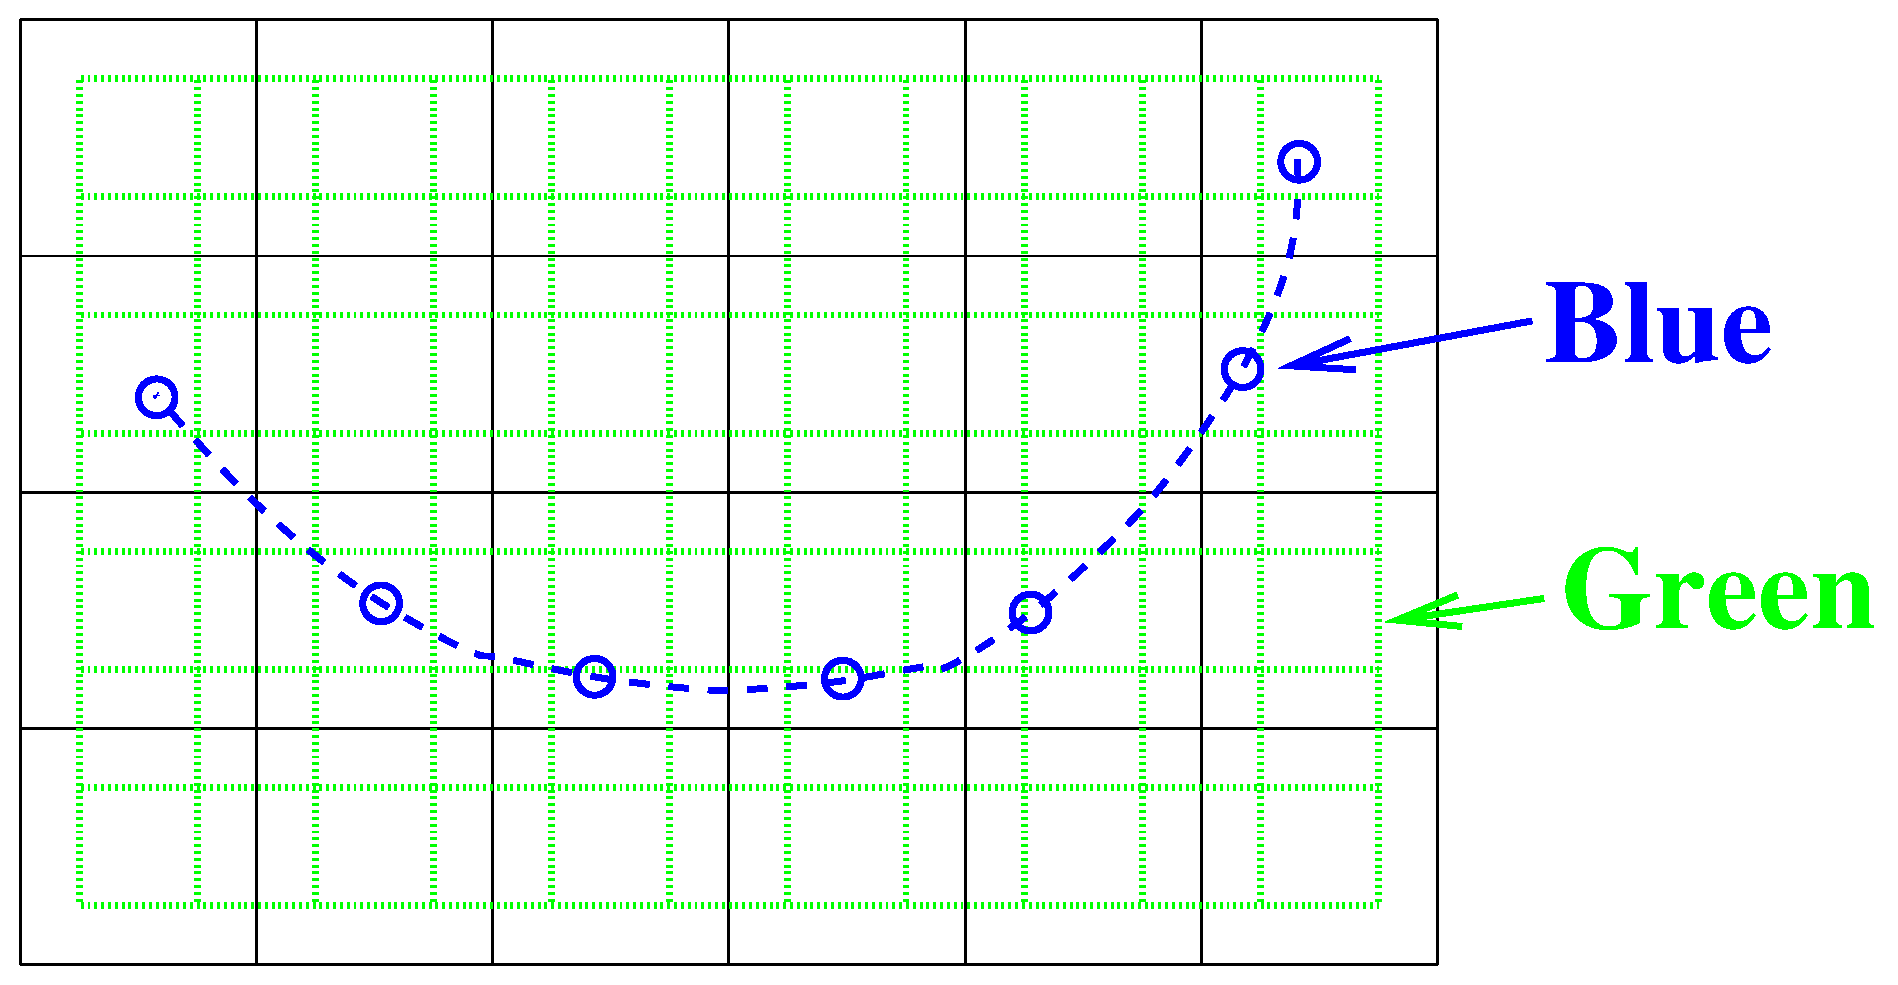
\includegraphics[width=.6\hsize]{interpolation/interpolation_types}
  \caption{The two different types of interpolation. Green (dotted):
    Interpolation to a new grid, output has same dimension as input,
    in this case 2D. Blue (dashed): Interpolation to a sequence of
    points, output is always 1D.}
  \label{fig:interpolation:types}
\end{figure}

There are two different types of interpolation in ARTS:
\begin{description}
\item[\textindex{Green Interpolation}:] Interpolation of a gridded field to a new
  grid.
\item[\textindex{Blue Interpolation}:] Interpolation of a gridded field to a
  sequence of positions.
\end{description}
Figure \ref{fig:interpolation:types} illustrates the different types
for a 2D example. 

The first step of an interpolation always consists in determining
where your new points are, relative to the original grid. You can do
this separately for each dimension. The positions have to be stored
somehow, which is described in the next section.



\levelb{Grid positions}
%-------------------------------------------------------------------------
\label{sec:interpolation:gridpos}

A grid position specifies where an interpolation point is, relative
to the original grid. It consists of three parts, an \artsstyle{Index} giving the
original grid index below the interpolation point, a \artsstyle{Numeric}
giving the fractional distance to the next original grid point, and a
\artsstyle{Numeric} giving 1 minus this number. Of course, the last element is
redundant. However, it is efficient to store this, since it is used
many times over. We store the two numerics in a plain C array of
dimension 2. (No need to use a fancy Array or Vector for this, since
the dimension is fixed.) So the structure \structindex{GridPos} looks like:

\begin{verbatim}
struct GridPos  {
   Index   idx;      /*!< Original grid index below
                          interpolation point. */
   Numeric fd[2];    /*!< Fractional distance to next point
                          (0<=fd[0]<=1), fd[1] = 1-fd[0]. */ 
};
\end{verbatim}

For example, \artsstyle{idx}=3 and \artsstyle{fd}=0.5 means that this interpolation point is
half-way between index 3 and 4 of the original grid.  Note, that
`below' in the first paragraph means `with a lower index'. If the
original grid is sorted in descending order, the value at the grid
point below the interpolation point will be numerically higher than
the interpolation point.  In other words, grid positions and
fractional distances are defined relative to the order of the original
grid. Examples:

{\small
\begin{verbatim}
old grid = 2 3
new grid = 2.25
idx      = 0
fd[0]    = 0.25

old grid = 3 2
new grid = 2.25
idx      = 0
fd[0]    = 0.75
\end{verbatim}
}

Note that \artsstyle{fd[0]} is different in the second case, because the old grid
is sorted in descending order. Note also that \artsstyle{idx} is the same in
both cases.

Grid positions for a whole new grid are stored in an \artsstyle{Array<GridPos>}
(called \artsstyle{ArrayOfGridPos}). 

\levelb{Setting up grid position arrays}
%----------------------------------------------------------------------

There is only one function to set up grid position arrays, namely 
\funcindex{gridpos}:

{\small
\begin{verbatim}
void gridpos( ArrayOfGridPos& gp,
              ConstVectorView old_grid,
              ConstVectorView new_grid );
\end{verbatim}
}

\hspace{-\parindent}Some points to remember:
\begin{itemize}
\item As usual, the output \artsstyle{gp} has to have the right dimension. 
  
\item The old grid has to be strictly sorted. It can be in ascending
  or descending order. But there must not be any duplicate values.
  Furthermore, the old grid must contain at least two points.
  
\item   The new grid does not have to be sorted, but the function will be
  faster if it is sorted or mostly sorted. It is ok if the new grid
  contains only one point.
  
\item   The beauty is, that this is all it needs to do also interpolation in
  higher dimensions: You just have to call gridpos for all the
  dimensions that you want to interpolate.
  
\item   Note also, that for this step you do not need the field itself at
  all!
\end{itemize}

\levelb{\textindex{Interpolation weights}}
%----------------------------------------------------------------------

As explained in the `Numerical Recipes'
\citep{numerical_recipes_C:97}, 2D bi-linear interpolation means, that
the interpolated value is a weighted average of the original field at
the four corner points of the grid square in which the interpolation
point is located. For simplicity, we label the four corner points
counterclockwise, starting from the lower left point (Figure
\ref{fig:interpolation:square}).  Then the interpolated value is given
by:
\begin{eqnarray}
  y(t,u)
  &=& (1-t)*(1-u)*y_1 \nonumber \\
  & & \mbox{} + t*(1-u)*y_2 \nonumber \\
  & & \mbox{} + t*u*y_3 \nonumber \\
  & & \mbox{} + (1-t)*u*y_4 \nonumber \\
  &=& w_1*y_1 + w_2*y_2 + w_3*y_3 + w_4*y_4
\label{eq:interpolation:weights}
\end{eqnarray}
where $t$ and $u$ are the fractional distances between the
corner points in the two dimensions, $y_i$ are the field values
at the corner points, and $w_i$ are the interpolation weights.

\begin{figure}
  \centering
  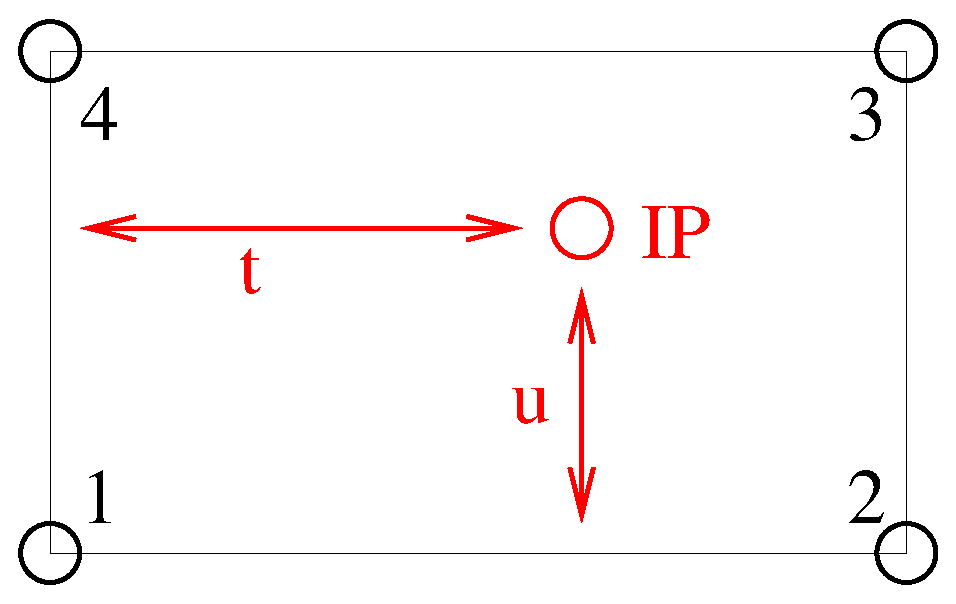
\includegraphics[width=.4\hsize]{interpolation/interpolation_square}
  \caption{The grid square for 2D interpolation. The numbers 1\ldots 4
    mark the corner points, IP is the interpolation point, $t$ and $u$
    are the fractional distances in the two dimensions.}
  \label{fig:interpolation:square}
\end{figure}

(By the way, I have discovered that this is exactly the result that
you get if you first interpolate linearly in one dimension, then in
the other. I was playing around with this a bit, but it is the more
efficient way to pre-calculate the $w_i$ and do all dimensions at once.

How many interpolation weights one needs for a multilinear
interpolation depends on the dimension of the interpolation: There are
exactly $2^n$ interpolation weights for an $n$ dimensional
interpolation.  These weights have have to be computed for each
interpolation point (each grid point of the new grid, if we do a
`green' type interpolation. Or each point in the sequence, if we do a
`blue' type interpolation).

This means, calculating the interpolation weights is not exactly
cheap, especially if one interpolates simultaneously in many
dimensions. On the other hand, one can save a lot by re-using the
weights.  Therefore, interpolation weights in ARTS are stored in a
tensor which has one more dimension than the output field. The last
dimension is for the weight, so this last dimension has the extent 4
in the 2D case, 8 in the 3D case, and so on (always $2^n$).

In the case of a `blue' type interpolation, the weights are
always stored in a matrix, since the output field is always 1D (a
vector). 

\levelb{Setting up interpolation weight tensors}
%----------------------------------------------------------------------

Interpolation weight tensors can be computed by a family of functions,
which are all called \funcindex{interpweights}. Which function is actually
used depends on the dimension of the input and output quantities. For
this step we still do not need the actual fields, just the grid
positions.

\levelc{Blue interpolation}

In this case the functions are:

{\small
\begin{verbatim}
void interpweights( MatrixView itw,
                    const ArrayOfGridPos& cgp );
void interpweights( MatrixView itw,
                    const ArrayOfGridPos& rgp,
                    const ArrayOfGridPos& cgp );
void interpweights( MatrixView itw,
                    const ArrayOfGridPos& pgp,
                    const ArrayOfGridPos& rgp,
                    const ArrayOfGridPos& cgp );
void interpweights( MatrixView itw,
                    const ArrayOfGridPos& vgp,
                    const ArrayOfGridPos& sgp,
                    const ArrayOfGridPos& bgp,
                    const ArrayOfGridPos& pgp,
                    const ArrayOfGridPos& rgp,
                    const ArrayOfGridPos& cgp );
\end{verbatim}
}

In all cases, the dimension of \artsstyle{itw} must be consistent with the
given grid position arrays and the dimension of the interpolation
(last dimension $2^n$). Because the grid position arrays are
interpreted as defining a sequence of positions they must all have
the same length.

\levelc{Green interpolation}

In this case the functions are:

{\small
\begin{verbatim}
void interpweights( Tensor3View itw,
                    const ArrayOfGridPos& rgp,
                    const ArrayOfGridPos& cgp );
void interpweights( Tensor4View itw,
                    const ArrayOfGridPos& pgp,
                    const ArrayOfGridPos& rgp,
                    const ArrayOfGridPos& cgp );
void interpweights( Tensor5View itw,
                    const ArrayOfGridPos& bgp,
                    const ArrayOfGridPos& pgp,
                    const ArrayOfGridPos& rgp,
                    const ArrayOfGridPos& cgp );
void interpweights( Tensor6View itw,
                    const ArrayOfGridPos& sgp,
                    const ArrayOfGridPos& bgp,
                    const ArrayOfGridPos& pgp,
                    const ArrayOfGridPos& rgp,
                    const ArrayOfGridPos& cgp );
void interpweights( Tensor7View itw,
                    const ArrayOfGridPos& vgp,
                    const ArrayOfGridPos& sgp,
                    const ArrayOfGridPos& bgp,
                    const ArrayOfGridPos& pgp,
                    const ArrayOfGridPos& rgp,
                    const ArrayOfGridPos& cgp );
\end{verbatim}
}

In this case the grid position arrays are interpreted as defining the
grids for the interpolated field, therefore they can have different
lengths. Of course, \artsstyle{itw} must be consistent with the length of
all the grid position arrays, and with the dimension of the
interpolation (last dimension $2^n$).

\levelb{The actual interpolation}
%----------------------------------------------------------------------

For this final step we need the grid positions, the
interpolation weights, and the actual fields. For each interpolated
value, the weights are applied to the appropriate original field values
and the sum is taken (see Equation
\ref{eq:interpolation:weights}). The \funcindex{interp} family of functions
performs this step.

\levelc{Blue interpolation}

{\small
\begin{verbatim}
void interp( VectorView            ia,
             ConstMatrixView       itw,
             ConstVectorView       a,    
             const ArrayOfGridPos& cgp);
void interp( VectorView            ia,
             ConstMatrixView       itw,
             ConstMatrixView       a,    
             const ArrayOfGridPos& rgp,
             const ArrayOfGridPos& cgp);
void interp( VectorView            ia,
             ConstMatrixView       itw,
             ConstTensor3View      a,    
             const ArrayOfGridPos& pgp,
             const ArrayOfGridPos& rgp,
             const ArrayOfGridPos& cgp);
void interp( VectorView            ia,
             ConstMatrixView       itw,
             ConstTensor4View      a,    
             const ArrayOfGridPos& bgp,
             const ArrayOfGridPos& pgp,
             const ArrayOfGridPos& rgp,
             const ArrayOfGridPos& cgp);
void interp( VectorView            ia,
             ConstMatrixView       itw,
             ConstTensor5View      a,    
             const ArrayOfGridPos& sgp,
             const ArrayOfGridPos& bgp,
             const ArrayOfGridPos& pgp,
             const ArrayOfGridPos& rgp,
             const ArrayOfGridPos& cgp);
void interp( VectorView            ia,
             ConstMatrixView       itw,
             ConstTensor6View      a,    
             const ArrayOfGridPos& vgp,
             const ArrayOfGridPos& sgp,
             const ArrayOfGridPos& bgp,
             const ArrayOfGridPos& pgp,
             const ArrayOfGridPos& rgp,
             const ArrayOfGridPos& cgp);
\end{verbatim}
}

\levelc{Green interpolation}

{\small
\begin{verbatim}
void interp( MatrixView            ia,
             ConstTensor3View      itw,
             ConstMatrixView       a,   
             const ArrayOfGridPos& rgp,
             const ArrayOfGridPos& cgp);
void interp( Tensor3View           ia,
             ConstTensor4View      itw,
             ConstTensor3View      a,   
             const ArrayOfGridPos& pgp,
             const ArrayOfGridPos& rgp,
             const ArrayOfGridPos& cgp);
void interp( Tensor4View           ia,
             ConstTensor5View      itw,
             ConstTensor4View      a,   
             const ArrayOfGridPos& bgp,
             const ArrayOfGridPos& pgp,
             const ArrayOfGridPos& rgp,
             const ArrayOfGridPos& cgp);
void interp( Tensor5View           ia,
             ConstTensor6View      itw,
             ConstTensor5View      a,   
             const ArrayOfGridPos& sgp,
             const ArrayOfGridPos& bgp,
             const ArrayOfGridPos& pgp,
             const ArrayOfGridPos& rgp,
             const ArrayOfGridPos& cgp);
void interp( Tensor6View           ia,
             ConstTensor7View      itw,
             ConstTensor6View      a,   
             const ArrayOfGridPos& vgp,
             const ArrayOfGridPos& sgp,
             const ArrayOfGridPos& bgp,
             const ArrayOfGridPos& pgp,
             const ArrayOfGridPos& rgp,
             const ArrayOfGridPos& cgp);
\end{verbatim}
}

\levelb{Examples}
%----------------------------------------------------------------------

\levelc{A simple example}

This example is contained in file \fileindex{test\_interpolation.cc}.

{\small
\begin{verbatim}
void test05()
{
  cout << "Very simple interpolation case\n";

  Vector og(1,5,+1);            // 1, 2, 3, 4, 5
  Vector ng(2,5,0.25);          // 2.0, 2,25, 2.5, 2.75, 3.0

  cout << "Original grid:\n" << og << "\n";
  cout << "New grid:\n" << ng << "\n";

  // To store the grid positions:
  ArrayOfGridPos gp(ng.nelem());

  gridpos(gp,og,ng);
  cout << "Grid positions:\n" << gp;

  // To store interpolation weights:
  Matrix itw(gp.nelem(),2);
  interpweights(itw,gp);
    
  cout << "Interpolation weights:\n" << itw << "\n";

  // Original field:
  Vector of(og.nelem(),0);
  of[2] = 10;                   // 0, 0, 10, 0, 0

  cout << "Original field:\n" << of << "\n";

  // Interpolated field:
  Vector nf(ng.nelem());

  interp(nf, itw, of, gp);

  cout << "New field:\n" << nf << "\n";
}
\end{verbatim}
}

\hspace{-\parindent}Ok, maybe you think this is not so simple, but a
large part of the code is either setting up the example grids and
fields, or output. And here is how the output looks like:

{\small
\begin{verbatim}
Very simple interpolation case
Original grid:
  1   2   3   4   5
New grid:
  2 2.25 2.5 2.75   3
Grid positions:
   1 0    1
   1 0.25 0.75
   1 0.5  0.5
   1 0.75 0.25
   1 1    0
Interpolation weights:
  1   0
0.75 0.25
0.5 0.5
0.25 0.75
  0   1
Original field:
  0   0  10   0   0
New field:
  0 2.5   5 7.5  10
\end{verbatim}
}

\levelc{A more elaborate example}

What if you want to interpolate only some dimensions of a tensor,
while retaining others? --- You have to make a loop yourself, but it
is very easy. Below is an explicit example for a more complicated
interpolation case. (Green type interpolation of all pages of a
Tensor3.) This example is also contained in file
\artsstyle{test\_interpolation.cc}.

{\small
\begin{verbatim}
void test04()
{
  cout << "Green type interpolation of all "
       << "pages of a Tensor3\n";

  // The original Tensor is called a, the new one n. 

  // 10 pages, 20 rows, 30 columns, all grids are: 1,2,3
  Vector  a_pgrid(1,3,1), a_rgrid(1,3,1), a_cgrid(1,3,1); 
  Tensor3 a( a_pgrid.nelem(),
             a_rgrid.nelem(),
             a_cgrid.nelem() ); 
  a = 0;
  // Put some simple numbers in the middle of each page:
  a(0,1,1) = 10;
  a(1,1,1) = 20;
  a(2,1,1) = 30;

  // New row and column grids:
  // 1, 1.5, 2, 2.5, 3
  Vector  n_rgrid(1,5,.5), n_cgrid(1,5,.5); 
  Tensor3 n( a_pgrid.nelem(),
             n_rgrid.nelem(),
             n_cgrid.nelem() ); 

  // So, n has the same number of pages as a, 
  // but more rows and columns.

  // Get the grid position arrays:
  ArrayOfGridPos n_rgp(n_rgrid.nelem()); // For rows.
  ArrayOfGridPos n_cgp(n_cgrid.nelem()); // For columns.

  gridpos( n_rgp, a_rgrid, n_rgrid );
  gridpos( n_cgp, a_cgrid, n_cgrid );

  // Get the interpolation weights:
  Tensor3 itw( n_rgrid.nelem(), n_cgrid.nelem(), 4 );
  interpweights( itw, n_rgp, n_cgp );

  // Do a "green" interpolation for all pages of a:

  for ( Index i=0; i<a.npages(); ++i )
    {
      // Select the current page of both a and n:
      ConstMatrixView ap = a( i,
                              Range(joker), Range(joker) );
      MatrixView      np = n( i,
                              Range(joker), Range(joker) );

      // Do the interpolation:
      interp( np, itw, ap, n_rgp, n_cgp );

      // Note that this is efficient, because interpolation
      // weights and grid positions are re-used.
    }

  cout << "Original field:\n";
  for ( Index i=0; i<a.npages(); ++i )
      cout << "page " << i << ":\n"
           << a(i,Range(joker),Range(joker)) << "\n";

  cout << "Interpolated field:\n";
  for ( Index i=0; i<n.npages(); ++i )
      cout << "page " << i << ":\n"
           << n(i,Range(joker),Range(joker)) << "\n";
}
\end{verbatim}
}

\hspace{-\parindent}The output is:

{\small
\begin{verbatim}
Green type interpolation of all pages of a Tensor3
Original field:
page 0:
  0   0   0
  0  10   0
  0   0   0
page 1:
  0   0   0
  0  20   0
  0   0   0
page 2:
  0   0   0
  0  30   0
  0   0   0
Interpolated field:
page 0:
  0   0   0   0   0
  0 2.5   5 2.5   0
  0   5  10   5   0
  0 2.5   5 2.5   0
  0   0   0   0   0
page 1:
  0   0   0   0   0
  0   5  10   5   0
  0  10  20  10   0
  0   5  10   5   0
  0   0   0   0   0
page 2:
  0   0   0   0   0
  0 7.5  15 7.5   0
  0  15  30  15   0
  0 7.5  15 7.5   0
  0   0   0   0   0
\end{verbatim}
}

\levelb{Summary}
%----------------------------------------------------------------------

Now you probably understand better what was written at the very
beginning of this chapter, namely that doing an interpolation always
requires the chain of function calls:
\begin{enumerate}
\item \artsstyle{gridpos} (one for each interpolation dimension)
\item \artsstyle{interpweights}
\item \artsstyle{interp}
\end{enumerate}
If you are interested in how the functions really work, look in file
\artsstyle{interpolation.cc}. The documentation there is quite detailed.
When you are using interpolation, you should always give some thought
to whether you can re-use grid positions or even interpolation
weights. This can really save you a lot of computation time. For
example, if you want to interpolate several fields --- which are all
on the same grids --- to some position, you only have to compute the
weights once.


%%% Local Variables: 
%%% mode: latex 
%%% TeX-master: "uguide" 
%%% TeX-master: "uguide"
%%% End:


\levela{Integration functions}
%--------------------------------------------------------------------------
\label{sec:integration}

\starthistory
  220802 & Created and written by Sreerekha T.R.\\
\stophistory

%
% Introduction
%
A radiative transfer model which takes into account the effect of
scattering involves integration of certain quantities over the angles
of observation.  For example, from Sections
\ref{sec:scattering:solution_rte} and
\ref{sec:scattering:abs_vec_spt} it is clear that computing  
scattering cross-section  and scattering integral term requires
integration over zenith and azimuth directions. There are a wide range of
methods that can be used for numerical integration. They can be used
depending on various factors starting from how accurate the result
should be to the behaviour of the function. The one which is
implemented in ARTS is the trapezoidal integration method. 


\levelb{Implementation files}
%-------------------------------------------------------------------------
\label{sec:integration:files}

The integration functions can be found in the files:
\begin{itemize}
\item \artsstyle{math\_funcs.h}
\item \artsstyle{math\_funcs.cc}
\end{itemize}
The implementation function \artsstyle {AngIntegrate\_trapezoid}is
discussed in the second file. 

\levelb{Trapezoidal Integration}
%------------------------------------------------------------------------
\label{sec:integration:trapezoidal}

Trapezoidal Integration method comes under the Newton-Cotes formulas
where integration of a function is approximated by the area under the
curve described by the function.  Trapezoidal integration assumes that
the area under the curve is trapezoid.  

Trapezoidal rule : 
\begin{eqnarray}
\label{eq:trapezoidal_rule}
{\int_{x_1}^{x_2} f(x)dx}  = \frac{1}{2} h (f_1 + f_2) + O(h^3 f^{''})
\end{eqnarray}
This is a two-point formula ($x_1$ and $x_2$).  It is exact for
polynomials upto and including degree 1, i.e., f(x) = x. $O(h^3
f^{''})$ signifies how far is the true answer from the estimate. 

If we use eq. \ref{eq:trapezoidal_rule} $N - 1$ times, to do the
integration in the intervals $(x_1, x_2)$,  $(x_2, x_3)$, ...,
$(x_{N-1}, x_N)$, and then add the results, we obtain extended formula
for the integral from $x_1$ to $x_N$.

Extended Trapezoidal rule :
\begin{eqnarray}
\label{eq:ext_trapezoidal_rule}
{\int_{x_1}^{x_N} f(x)dx}  = \frac{1}{2} h \left [f_1 + 2(f_2 + f_3 +
... +f_{N-1})+f_N \right] + O\left [ \frac {(b-a)^3 f^{''}}{N^2} \right]
\end{eqnarray}

The last term tells how much the error will be decreased by taking
more number of steps. 

\levelb{Solid Angle Integration}
%------------------------------------------------------------------------
\label{sec:integration:solid_angle}
In our scattering problem, we are often encountered with a double integration
of functions over zenith and azimuth angles (see Chapter
\ref{sec:scattering}).  One way to achieve
double integration is to use repeated
one-dimensional trapezoidal integration.  This is effective of course
only if the boundary is simple and the function is very smooth.  If
the function is strongly peaked and if know where it occurs, integral
should be broken into smaller regions so that the 
integrand is smooth in each.  Another thing is to take into account
the symmetry of the function as well as the boundary. For example in
our case, if the radiation is symmetric about the azimuth, the
integration in that direction returns constant value of $2 \pi$ and we
need to do only integration over zenith directions.  

The function takes in as input the integrand and the angles over which
the integration has to be done. For example in this case it can be the
zenith and azimuth angle
grid.
\begin{verbatim}  
Numeric AngIntegrate_trapezoid(MatrixView Integrand,
                               ConstVectorView za_grid,
                               ConstVectorView aa_grid)
\end{verbatim}
The integrand has the same number of rows as zenith angle grid
and columns as azimuth angle grid.  The inner loop does trapezoidal
integration of the integrand over all azimuth angles and the result is
stored in a Vector  res1[i]. Note that the integrand at every point
has to be multiplied with \artsstyle {sin (za\_grid[i] * DEG2RAD)}
since we are integrating over solid angles.  The outer loop 
does an integration of res1[i] over all zentih angles.  The result of
this is returned back to the calling function.  


%%% Local Variables: 
%%% mode: latex
%%% TeX-master: t
%%% End: 

\chapter{Linear algebra functions}
%--------------------------------------------------------------------------
\zlabel{sec:lin_alg}

\starthistory
  020502 & Created and written by Claudia Emde.\\
\stophistory

%
% Introduction
%

Solving the vector radiative transfer equation requires the
computation of linear equation systems and the matrix
exponential. This section describes the functions which are implemented
in ARTS and it gives instructions how these functions can be used, also
for other purposes than the radiative transfer calculations.

\section{Implementation files}
%-------------------------------------------------------------------------
\zlabel{sec:lin_alg:files}

All the functions described below can be found in the files:
\begin{itemize}
\item \artsstyle{lin\_alg.h}
\item \artsstyle{lin\_alg.cc}
\end{itemize}
The template class \artsstyle{Array} and the classes \artsstyle{Matrix} and
\artsstyle{Vector} are used, therefore the linear algebra functions require
the files:
\begin{itemize}
\item \artsstyle{matpackI.h}
\item \artsstyle{make\_vector.h}
\item \artsstyle{array.h}
\item \artsstyle{matpackI.cc}
\item \artsstyle{make\_vector.cc}
\item \artsstyle{array.cc}
\end{itemize}
Furthermore logical functions contained in
\begin{itemize}
\item \artsstyle{logic.h}
\item \artsstyle{logic.cc}
\end{itemize}
are used to check the dimensions of input matrices for various functions.


\section{Linear Equation Systems}
%------------------------------------------------------------------------
\zlabel{sec:lin_alg:lineqsys}


For solving a set of linear equations 
\begin{eqnarray}
\zlabel{eq:lin_equ_sys}
{\bf A} {\bf x} = {\bf b}
\end{eqnarray}
the LU decomposition method is implemented.A slightly modified version
of the algorithm described in
[\cite{numerical_recipes_C:97}] is used here. An alternative method
is the Gauss-Jordan elimination, but this method is three times
slower than the LU decomposition method
[\cite{numerical_recipes_C:97}, p.36]. The LU decomposition method
reqires two functions, \artsstyle{ludcmp} and \artsstyle{lubacksub},
which will be decribed below.
\vspace{0.5cm}\\
The following example for a three dimensional equation sytem 
demonstrates how to solve a linear
equation sytem of the type
(\zref{eq:lin_equ_sys}):
\begin{itemize}
\item Create matrix A, vector b: \\
  \artsstyle{A = Matrix(3,3);} \\
  \artsstyle{A(1,1) = 4;}\\
  \artsstyle{A(2,1) = 3;}\\
  $\cdots$\\
  \artsstyle{b = Vector(3);}\\
  \artsstyle{b(1) = 7;}\\
  $\cdots$
\item Initialize solution vector x and two other variables needed for
  storing intermediate results:\\
  \artsstyle{x = Vector(3);}\\
  \artsstyle{LU = Matrix(3,3);}\\
  \artsstyle{indx = ArrayOfIndex(3);}
\item Call LU decomposition function (see Section \zref{sec:lin_alg:lu_decomp}): \\
  \artsstyle{ludcmp(LU, indx, A);}
\item Call LU backsubstitution function (see Section \zref{sec:lin_alg:backsub}): \\
  \artsstyle{lubacksub(x, LU, b, indx);}
\item Print the solution vector:\\
  \artsstyle{cout << x;}
\end{itemize}

\subsection{LU Decomposition}
%------------------------------------------------------------------------
\zlabel{sec:lin_alg:lu_decomp}

A LU decomposition is a procedure for decomposing a square matrix {\bf
  A} with
dimension $n$ into a product of a lower triangular matrix {\bf L} (has
elements only on the diagonal elements and below) and
an upper triangular matrix {\bf U} (has elements only on the diagonal
and above):
\begin{equation}
  \zlabel{eq:lu_decomp}
  {\bf L}\cdot{\bf U} ={\bf A} 
\end{equation}
For a 3 x 3 matrix equation \zref{eq:lu_decomp} would look like this: 
\[ \left(
  \begin{array}{ccc}
    l_{11} & 0 & 0 \\
    l_{21} & l_{22} & 0 \\
    l_{31} & l_{32} & l_{33}
    \end{array} \right)
\cdot
\left(
  \begin{array}{ccc}
    u{11} & u_{12} & u_{13} \\
    0 & u_{22} & u_{23}\\
    0 & 0 & u_{33}
    \end{array} \right)
=
\left(
  \begin{array}{ccc}
    a_{11} & a_{12} & a_{13} \\
    a_{21} & a_{22} & a_{23} \\
    a_{31} & a_{32} & a_{33}
    \end{array} \right)
\]
The decomposition can be used to rewrite the linear set of equations
(\zref{eq:lin_equ_sys}) in the following way:
\begin{eqnarray}
  {\bf A}\cdot{\bf x} = ({\bf L}\cdot{\bf U})\cdot{\bf x} = {\bf
    L}\cdot({\bf U}\cdot{\bf x}) = {\bf b}
\end{eqnarray}
First 
\begin{equation}
  {\bf L} \cdot{\bf y} = {\bf b}
\end{equation}
is solved for the vector ${\bf y}$ which can be done by
forward substitution (see section \zref{sec:lin_alg:backsub}). Then 
\begin{equation}
  {\bf U} \cdot{\bf x} = {\bf y}
\end{equation}
is solved again by backsubstitution. 
The advantage in breaking up one linear set into two successive ones
is that the solution of a triangular set of equations is quite trivial.

The function \artsstyle{ludcmp} requires a square matrix of arbitrary
dimension $n$ as input and performs the LU decomposition. It returns one
matrix which contains both matrices, ${\bf L}$ and ${\bf U}$. 
For the lower triangular matrix  ${\bf L}$ the diagonal elements 
are chosen to be 1, then the other elements of ${\bf L}$ and ${\bf U}$
are determined. This is possible, as the LU decomposition is an under
determined equation sytem with $n^2$ equations for $n^2+n$ unknowns. 
The output matrix does not include the diagonal of ${\bf L}$, in the
three-dimensional case it has the following elements:
\[ \left(
  \begin{array}{ccc}
    u_{11} & u_{12} & u_{13} \\
    l_{21} & u_{22} & u_{23} \\
    l_{31} & l_{32} & u_{33}
    \end{array} \right)
\]
This special arrangement of the LU decomposition is named {\sl
Crout's algorithm} and a matrix arranged in this form is named {\sl
Crout matrix} in this context.
  

Another output variable of the function \artsstyle{ludcmp} is an index
vector which contains information about pivoting which is absolutely
essential for the stability of
Crout's algorithm. Here partial pivoting,
i.e. interchange of rows is implemented. That means that not {\bf A} is
decomposed into $LU$-form but a rowwise permutation of {\bf A}. If the
index vector contains for example the elements $(2,1,0)$ the first and
the last row of a three dimensional matrix would be exchanged.


\subsection{Forward- and Backsubstitution}
%---------------------------------------------------------------
\zlabel{sec:lin_alg:backsub}
An equation system of the form
\[ 
\left(
  \begin{array}{ccc}
    a{11} & a_{12} & a_{13} \\
    0 & a_{22} & a_{23}\\
    0 & 0 & a_{33}
    \end{array} \right)
\cdot
\left(
  \begin{array}{c}
    x_1\\x_2\\x_3
 \end{array} \right)
=
\left(
  \begin{array}{c}
    b_1\\b_2\\b_3
 \end{array} \right)
\]
can be solved very easy. The last element, here $x_3$, is already isolated,
namely
\begin{eqnarray}
  x_3 = b_3/a_{33}
\end{eqnarray}
As $x_3$ is known $x_2$ can be calculated using the second row of the
eqautions. Then, finally, $x_1$ can be calculated as well using the
first row. This procedure
is called backsubtitution. The same
method  applied for an equation system including a
lower triangular matrix is named forward substitution.   

The function \artsstyle{lubacksub} does forward and backward
substitution to solve the equation system described in
\zref{sec:lin_alg:lu_decomp}. As input it requires the output variables of
\artsstyle{ludcmp} which are the {\sl Crout matrix} and the index
vector. Output of the function is the solution vector ${\bf x}$ to the
equation system.


\subsection{More Applications of the LU Decomposition}
%-------------------------------------------------------------------
\zlabel{lu_applications}

\begin{itemize}
\item Inverse of a matrix:\\
  To compute $(\bf K)^{-1}\cdot{\bf b}$, which is a part of the
solution to the vector radiative transfer equation (\zref{eq:scattering:VRTE_sol}) the LU
decomposition method can be used. The following equations show, that
the problem is equivalent to  solving a linear equation system of the type
\zref{eq:lin_equ_sys}.
\begin{eqnarray}
  {\bf K}^{-1}\cdot{\bf b} &=& {\bf x}\\
\Leftrightarrow \qquad  {\bf K}\cdot{\bf x} &=& {\bf b}
\end{eqnarray}

\item To solve the equation system
  \begin{eqnarray}
    {\bf A}\cdot{\bf X} &=& {\bf B}
  \end{eqnarray}
where {\bf A}, {\bf B} and  {\bf X} are matrices of dimension
$n$, the LU decomposition functions can be applied as well. Assume
that {\bf A} and {\bf B} are known and you want to solve for {\bf
 X}.
First you should do a LU decomposition of  {\bf A} and then
backsubstitute with the columns of B and you get the columns of {\bf
  X} as solution vectors.

\end{itemize}

\section{Matrix Exponential Function}
%----------------------------------------------------------------
\zlabel{sec:lin_alg:mat_exp}

A very important function for solving differential equations is the
matrix exponential:
\begin{eqnarray}
  \zlabel{eq:mat_exp}
  e^{{\bf A}s} = \sum_{k=0}^\infty{\frac{({\bf A} s)^k}{k!}}
\end{eqnarray}
In principle it could be computed using the Taylor power series but 
 this method is not efficient. {\sc Moler} and {\sc Van
  Loan} have shown for the simple example [\cite{Moler_Loan:79}]
\[ {\bf A} =
\left(
  \begin{array}{cc}
    -49 & 24\\
    -64 & 31
    \end{array} \right) \]
that convergence is obtained not until 59 terms. And if a relative
accuracy of only 10$^{-5}$ is taken, the method even leads to a wrong
result due to rounding errors.

\subsection{Pad\'e Approximation}
%----------------------------------------------------------------------
\zlabel{sec:pade_approximation}

One of the better algorithms for computing the matrix exponential is
the Pad\'e approximation which is also shortly described in
[\cite{Moler_Loan:79}] and outlined in the book ``Matrix
Computations'' by \cite{Golub_Loan:91}. 
The method uses perturbation theorie as well as the so called Pad\'e
functions. It is possible to derive an algorithm which calculates
\begin{eqnarray}
  {\bf F} = e^{{\bf A}+{\bf E}} 
\end{eqnarray}
where 
\begin{eqnarray}
  \|{\bf E}\|_\infty \le \delta \|{\bf A}\| .
\end{eqnarray}
The accuracy of the computation given by $\delta$ can be chosen. 
The parameter q has to be the smallest non-negative integer such that
$\epsilon(q,q)\le\delta$ where
\begin{eqnarray}
  \epsilon(p,q) = 2^{3-(p+q)}\frac{p!q!}{(p+q)!(p+q+1)!}.
\end{eqnarray}
The following table shows values of epsilon for
different values of q.
\vspace{0.5cm}\\
\begin{tabular}[h]{|r|r|}
 \hline
q & $\epsilon$(q,q) \\ \hline
1 & 0.1667\\
2 & 6.9444 $\cdot$ 10$^{-4}$ \\
3 & 1.2401 $\cdot$ 10$^{-6}$ \\
4 & 1.2302 $\cdot$ 10$^{-9}$ \\
5 & 7.7667 $\cdot$ 10$^{-13}$ \\
6 & 3.3945 $\cdot$ 10$^{-16}$ \\ 
\hline
\end{tabular}
\vspace{0.5cm}\\
The algorithm is implemented in the function \artsstyle{matrix\_exp}. Input
to this function is the matrix ${\bf A}$ and the parameter $q$. As output
it gives the matrix ${\bf F}$ which is defined above.\\
The following example shows how to use the \artsstyle{matrix\_exp} function:
\begin{itemize}
\item Initialize {\bf A} and assign values:\\
  \artsstyle{Matrix A(3,3);}\\
  \artsstyle{A(1,1) = 45;}\\
  \artsstyle{A(1,2) = 3;}\\
$\cdots$ 
\item Initialize {\bf F}:\\
  \artsstyle{Matrix F(3,3);}
\item Give a paramater for the accuracy:\\
  \artsstyle{Index q=6;}
\item Call the matrix exponential function:\\
  \artsstyle{matrix\_exp(F,A,q);}
\item Print the result: \\
  \artsstyle{cout << "exp(A) = " << F;}
\end{itemize}






%%% Local Variables: 
%%% mode: latex
%%% TeX-master: t
%%% End: 

%
\part{Theoretical background}
\chapter{Basic radiative transfer theory}
 \label{sec:rte_theory}


\starthistory
  030305 & Copied from a compendium written by Patrick Eriksson.\\
\stophistory


 When dealing with atmospheric radiation a division can be made
 between two different wavelength ranges where the limit is found
 around 5 $\mu$m, i.e. one range consists of the near IR, visible and UV
 regions while the second range covers thermal and far IR and
 microwaves. The first reason to this division is the principal
 sources to the radiation in the two ranges, for wavelengths shorter
 than 5 $\mu$m the solar radiation is dominating while at longer
 wavelengths the thermal emission from the surface and the atmosphere
 is more important. A second reason is the importance of scattering
 but here it is impossible to give a fixed limit. Clouds are important
 scattering objects for most frequencies but at cloud free conditions
 scattering can in many cases be neglected for wavelengths $>$ 5 $\mu$m. If
 the atmosphere can be assumed to be in local thermodynamic
 equilibrium the radiative transfer can be simplified considerably,
 and this is a valid assumption for the IR region and microwaves but
 not for e.g. UV frequencies.
 
 The radiative transfer in the atmosphere must be adequately described
 in many situations, as when estimating rates of photochemical
 reactions, calculating radiative forcing in the atmosphere or
 evaluating an remote sensing observation. It is not totally
 straightforward to quantify the radiative transfer with good accuracy
 because the calculations can be very computationally demanding and
 many of the parameters needed are hard to determine. For example,
 situations when a great number of transitions or multiple scattering
 must be considered will cause long calculations while as a rule
 scattering is problematic to model because the shape and size
 distribution of the scattering particles are highly variable
 quantities.  
 
 If scattering can be neglected and the atmosphere is assumed to be in
 local thermodynamic equilibrium, the radiative transfer equation gets
 unusually simple. These assumptions will be made below and
 they are normally valid for the infrared region and longer
 wavelengths as in the microwave region. For these conditions the
 atmospheric absorption and emission are linked and the basic problem
 to determine the radiative transfer is to calculate the absorption.
 At the wavelengths considered rotational and vibrational transitions
 are the dominating absorbing processes.


\section{Blackbody radiation}
 \label{sec:rtetheory:planck}
 
 All natural bodies with a temperature $>$ 0 K emit thermal radiation.
 The thermal motion in the matter is translated by collisions to
 excitations in the molecules. The transition from the excited state
 to a lower state causes emission of electromagnetic radiation.
 Depending on the temperature the distribution of the emission will
 change. An ideal body that absorbs all incoming radiation is called a
 blackbody and its emittance follows Planck's formula: 

 \begin{equation}
   B(\lambda,T) = \frac{2\pi hc^2}{\lambda^5} \frac{1}{e^{hc/\lambda k_bT}-1}
  \label{eq:rtetheory:planck}
 \end{equation}
 where $B$ is the emitted radiation, $\lambda$ the wavelength, $T$ the 
 temperature, $h$ the Planck constant, $c$ the speed of light and $k_b$
 the Boltzmann constant. Equation~\ref{eq:rtetheory:planck} is shown in Figure 
 \ref{fig:rtetheory:planck} for some temperatures.

 \begin{figure}
  \begin{center}
   \includegraphics*[width=0.8\hsize]{rte_theory/fig_planck}
    \caption{The blackbody radiation as a function of wavelength for
             some temperatures.}
    \label{fig:rtetheory:planck}
  \end{center}
 \end{figure}   
                                       
 The maximum of the Planck formula is a function temperature and is
 given by the Wien's displacement law. The maximum of
 Equation~\ref{eq:rtetheory:planck} is found at: 

 \begin{equation}
   \lambda_{max} = \frac{K}{T}
  \label{eq:rtetheory:wien}
 \end{equation}
 where is $\lambda_{max}$ the wavelength of maximum emittance and $K
 =$~2.898\topowerten{-3} Km. Consequently the maximum is encountered
 at a shorter wavelength for a higher temperature as can be seen in
 Figure \ref{fig:rtetheory:planck}.
                                     
 No natural object can be said to be a perfect blackbody but the Sun
 and the Earth can approximately be treated as blackbodies with
 temperature of about 6000 and 290 K, respectively, to explain some
 basic conditions. Wien's displacement law gives maximum for the solar
 radiation at 0.55 $\mu$m while the Earth thermal radiation is maximal
 around 10 $\mu$m. The solar maximum coincides with a region of high
 atmospheric transmission and this explains why the
 evolution has placed the vision between about 400 - 700 nm, the
 amount of energy at surface level is maximal in this range.  
 
 If the radiation from the Sun is scaled to compensate for the
 attenuation due to the distance it will be found that the radiation
 from the Earth itself will dominate for wavelengths longer than about
 5 $\mu$m. This means, for example, that remote sensing techniques in
 the thermal IR and microwave region primarily detect thermal emission
 from the surface or the atmosphere while observations in the optical
 and UV regions use absorbed, scattered or reflected solar radiation.
 This also explains why gases that exhibit absorption between 5 - 50
 $\mu$m are called greenhouse gases, they absorb partly some of the
 outgoing radiation from the surface and the sea.


\section{General theory}
 \label{sec:rtetheory:gen_theory}

 The basic equation describing radiative transfer along a specific 
 direction is

 \begin{equation}
   \frac{dI(\nu)}{dl} = -k(l,\nu)I(\nu) + S(l,\nu)
  \label{eq:rtetheory:chand}
 \end{equation} 
 where $I$ is the intensity per unit area, $\nu$ the frequency, $l$
 the distance along the propagation path, $k$ the total absorption
 coefficient (summed over all species and transitions) and $S$ the
 source term. In this general expression both $k$ and $S$ include
 effects of scattering, i.e. energy lost and gained in the viewing
 direction due to scattering. The discussion will here be restricted
 to situations where the scattering can be neglected. This can be a
 valid assumption for cloud free conditions and wavelengths greater
 than a few micrometers. At microwave wavelengths scattering can
 normally be neglected also when clouds are present. For the
 frequencies considered and altitudes below about 75 km the molecules
 in the atmosphere can also be considered to be in local thermodynamic
 equilibrium. This implies that the de-excitation and excitation of a
 transition have the same probability and the absorption and emission
 coefficients will be equal.  The Kirchoff law then states that the
 emitted radiance, the source function, is

 \begin{equation}
   S = k(l,\nu)B(T(l),\nu)
  \label{eq:rtetheory:kirch}
 \end{equation}  
 For the conditions given, no scattering and local thermodynamic
 equilibrium, the radiative transfer equation is obtained by combining
 Equations \ref{eq:rtetheory:chand} and \ref{eq:rtetheory:kirch}. The resulting
 differential equation can be solved to give

 \begin{equation}
   I(\nu) = I_0(\nu)e^{-\int^h_0{k(l',\nu)dl'}} + 
     \int^h_0{k(l,\nu)B(T(l),\nu) e^{-\int^l_0{k(l',\nu)dl'}} dl}
  \label{eq:rtetheory:rte}
 \end{equation}  
 where the receiver is assumed to be placed at $l$~=~0 and $h$ is the
 distance along the path to the limit of the media. $I_0$ is the
 intensity at the point $h$ which can represent thermal emission from
 the surface, solar radiation at top of the atmosphere or cosmic
 background radiation depending on the observation geometry. When
 discussing radiative transfer the quantity optical depth, $\tau$, is
 commonly used and it is defined as

 \begin{equation}
   \tau(l,\nu) = \int^l_0{k(l',\nu)dl'} 
  \label{eq:rtetheory:tau}
 \end{equation}  
 and Equation \ref{eq:rtetheory:rte} can be written as
 
 \begin{equation}
   I(\nu) = I_0(\nu)e^{-\tau(h,\nu)dl'} + 
     \int^h_0{k(l,\nu)B(T(l),\nu) e^{-\tau(l',\nu)} dl}
  \label{eq:rtetheory:rte2}
 \end{equation}  
 The terms inside the integral found in this equation have a simple
 physical meaning, the radiation emitted at one point is $kBdl$ and this
 quantity is attenuated by the factor $e^{-\tau}$ before it reaches the
 observation point.


\section{Special solutions}
 \label{sec:rtetheory:special}
 
 If the total emission along the propagation path can be neglected
 compared to the transmitted part of the incoming radiation, the
 radiative transfer equation is simplified to the well known Beer-Lambert law:
 
 \begin{equation}
   I(\nu) = I_0(\nu)e^{-\tau(h,\nu)}
  \label{eq:rtetheory:beer}
 \end{equation}  
 This equation can for example be used when evaluating solar
 occultation observations.  
 
 If the temperature is constant through the medium studied (Fig.
 \ref{fig:rtetheory:layer}) the integral in Equation \ref{eq:rtetheory:rte} can be solved
 analytically:

 \begin{figure}
  \begin{center}
   \begin{minipage}[c]{0.4\textwidth}
    \centering
    \caption{Schematic picture of the radiative transfer through a medium with
             constant temperature.}
    \label{fig:rtetheory:layer}
   \end{minipage}%
   \hspace{0.05\textwidth}%
   \begin{minipage}[c]{0.50\textwidth}
    \centering
    \includegraphics*[width=0.99\hsize]{rte_theory/fig_layer}
   \end{minipage}
  \end{center}
 \end{figure}   
  
 \begin{equation}
   I^{out} = I^{in}e^{-\tau} + B(T,\nu)(1-e^{-\tau})
  \label{eq:rtetheory:layer}
 \end{equation}  
 where is $\tau$ the total optical thickness of the medium. Two
 special cases can be distinguished. If the layer is totally optically
 thick ($\tau \to \infty$) then $I^{in}$ is totally absorbed and
 $I^{out} = B$, the medium emits as a blackbody. If the layer has no
 absorption ($\tau=0$) then Equation \ref{eq:rtetheory:layer} gives
 $I^{out} = I^{in}$ as expected.
 
 In microwave radiometry the measured intensity is normally presented
 by means of the brightness temperature, $T_b$. This quantity is
 derived from the Rayleigh-Jeans approximation of the Planck function:

 \begin{equation}
   B(T,\nu) \approx \frac{2\nu^2k_bT}{c^2} = \frac{2k_bT}{\lambda^2}
  \label{eq:rtetheory:rayjean}
 \end{equation}  
 This equation is valid when $h\nu \ll kT$ which is the case in the
 microwave region due to the relatively low frequencies. If the
 temperature is 50 K, $hv$ equals $kT$ at 1.04 THz. The important
 aspect of Equation \ref{eq:rtetheory:rayjean} is the linear relationship
 between the intensity and the physical temperature. The natural
 definition of brightness temperature, $T_b$, is then

 \begin{equation}
   T_b(\nu) = \frac{\lambda^2}{2k_bT} I(\nu)
  \label{eq:rtetheory:tb}
 \end{equation}  
 The difference between the brightness temperature and the physical
 temperature (corresponding to the actual intensity) increases with
 frequency which is exemplified in Figure \ref{fig:rtetheory:rayjean}. The
 differences for higher frequencies are certainly not negligible and
 the brightness temperature shall not be mistaken for the physical
 temperature. The important fact is that the brightness temperature
 has a linear relationship to the intensity and gives a more intuitive
 understanding of the magnitude of the emission. In the Rayleigh-Jeans
 limit Equation \ref{eq:rtetheory:rte} can be written as

 \begin{equation}
   T_b(\nu) = T_{b0}(\nu)e^{-\tau(h,\nu)dl'} + 
     \int^h_0{k(l,\nu)T(l) e^{-\tau(l',\nu)} dl}
  \label{eq:rtetheory:rte_tb}
 \end{equation}  

 \begin{figure}
  \begin{center}
    \includegraphics*[width=0.8\hsize]{rte_theory/fig_rayjean}
    \caption{The difference between the physical temperarature of a 
             blackbody and the equivalent brightness temperature
             calculated using the Rayleight-Jeans approximation.}
    \label{fig:rtetheory:rayjean}
  \end{center}
 \end{figure}   

\chapter{Polarisation and Stokes parameters}
 \label{sec:polarization}


\starthistory
  040524 & Section on scattering matrices added by Patrick Eriksson. \\
  040426 & Created and written by Christian Melsheimer.\\
\stophistory


\graphicspath{{Figs/polarization/}}



%=====================================================================
% Definition of new commands:
% ====================================================================
% a 3-elem. column vector:
\newcommand{\ColVct}[3]{\left( \begin{array}{c}
                                   #1 \\ #2 \\ #3
                               \end{array} \right) }
% partial derivative of #1 with respect to #2, written as a fraction:
\newcommand{\PrtDrv}[2]{\frac{\partial #1}{\partial #2}}
%\newcommand{\half} {\ensuremath{\textstyle\frac{1}{2}}}
%Inverse Wave Impendance
%\newcommand{\InvImp} %
%      {\ensuremath{\sqrt{\textstyle{\frac{\epsilon}{\mu}}}}}
% various polarization basis vectors:
\newcommand{\eVrt} {\ensuremath{\VctStl{e}_v}}
\newcommand{\eHor} {\ensuremath{\VctStl{e}_h}}
\newcommand{\eLh} {\ensuremath{\VctStl{e}_{LH}}}
\newcommand{\eRh} {\ensuremath{\VctStl{e}_{RH}}}
\newcommand{\ePls} {\ensuremath{\VctStl{e}_{+45\degree}}}
\newcommand{\eMin} {\ensuremath{\VctStl{e}_{-45\degree}}}
\newcommand{\mi}  {\ensuremath{\mathrm{i}}}


The present version of ARTS implements the radiative transfer equation in
tensor form, i.e., for the 4 components of the Stokes vector, not just for its
first component, the intensity or radiance. This means that the model can
include polarisation dependence in absorption or scattering processes. It is
therefore necessary to give some details on the polarisation of radiation, the
definition of the Stokes parameters, and the definition of antenna
polarisation.\\

\noindent {\color{red} This section could need to be revised. At least there is
  an inconsisteny regarding the V-element between this section and what is
  written elsewhere. In this section V is said to be righ-hand minus left-hand
  circular polarisation, while elsewehere it is the opposite.}


\section{Polarisation directions}
%=====================================================================
\label{sec:polarization:directions}
Electromagnetic waves in homogeneous, isotropic media are transverse
waves, i.e., their oscillating electric and magnetic fields are in a
plane perpendicular to the propagation direction. The choice of two
basis vectors -- we shall call them polarisation directions here --
that span that transverse plane is arbitrary; often they are called
``horizontal'' and ``vertical'' and correspond to some horizontal and
vertical direction of the particular setting. Nevertheless, what is
meant by horizontal/vertical, or parallel/perpendicular, is purely a
matter of definition.

Here, we stick to the system called laboratory frame or fixed frame, used by
\citet{Mishchenko:02}: We use a coordinate system where the $z$-axis points
toward local zenith. We denote the propagation direction of radiation by a unit
vector $\VctStl{n} = \VctStl{k}/k$, where $k$ is the wave number. $\VctStl{n}$
is given by two angles, the zenith angle $\theta$ , i.e., the angle between
$\VctStl{n}$ and the $z$-axis, and the azimuth angle $\phi$, i.e., the angle
between the projection of $\VctStl{n}$ into the $xy$-plane and the $x$-axis:
\begin{equation}
  \label{eq:polarization:propdir}
   \VctStl{n} = \ColVct{\cos\phi \sin\theta}%
                       {\sin\phi \sin\theta}%
                       { \cos\theta}                    
\end{equation}
Then we define the polarisation directions by the partial derivatives
of  $\VctStl{n}$ with respect to $\theta$ and $\phi$. We shall call
them $\theta$-direction (also: vertical) and $\phi$-direction (also:
horizontal), respectively, see
Figure \ref{fig:polarization:directions}. 
\begin{figure}
 \begin{center}
  \begin{minipage}[c]{0.9\textwidth}
   \begin{center}
    \includegraphics*[width=0.9\hsize]{pol_directions}
   \end{center}
  \end{minipage}
  \begin{minipage}[c]{0.9\textwidth}
   \caption{The definition of the polarisation directions, adapted
     from \citet{Mishchenko:02}}
   \label{fig:polarization:directions}
  \end{minipage}
 \end{center}
\end{figure}   
%
Their unit basis vectors are
\begin{equation}
  \label{eq:polarization:etheta}
   \VctStl{e}_\theta = \eVrt =
    \PrtDrv{\VctStl{n}}{\theta} \left/ 
     \left\| \PrtDrv{\VctStl{n}}{\theta}\right\| \right.  
    =
    \ColVct{\cos\phi \cos\theta}%
           {\sin\phi \cos\theta}%
           { -\sin\theta}
\end{equation}
%
\begin{equation}
  \label{eq:polarization:ephi}
   \VctStl{e}_\phi = \eHor = 
    \PrtDrv{\VctStl{n}}{\phi} \left/ 
          \left\|\PrtDrv{\VctStl{n}}{\phi}\right\| \right.  
    =
    \ColVct{-\sin\phi}%
           {\cos\phi}%
           { 0}
\end{equation}
The vectors \VctStl{n}, $\VctStl{e}_\theta$ (=\eVrt),
$\VctStl{e}_\phi$ (=\eHor) are
mutually orthogonal and define (in the mentioned order) a right-handed
system, i.e., 
$\left(\VctStl{n}\times \VctStl{e}_\theta\right) \cdot
\VctStl{e}_\phi = 1$ and the same for all cyclic permutations.


\section{Plane monochromatic waves}
%=====================================================================
\label{sec:polarization:monochrom}

Plane monochromatic electromagnetic waves are commonly written in the form
\begin{equation} 
  \label{eq:polarization:e_field}
  \VctStl{E}(\VctStl{x},t) 
   = \left[E_v \atop E_h\right] e^{i(\VctStl{k}\VctStl{x} - \omega t)}
   = \left(E_v \eVrt +  E_h \eHor \right) 
      e^{i(\VctStl{k}\VctStl{x} - \omega t)}
\end{equation}
where $\VctStl{E}$ is the electric field vector, the subscripts $v$
and $h$ denote the components with vertical and horizontal
polarisation, respectively. $E_v$ and $E_h$, the amplitudes, are
complex numbers, $\VctStl{k}$ and $\omega$ are the wavenumber vector
and the angular frequency, respectively, of the plane wave, and the
unit vectors $\eVrt = (1,0)\Trp$, $\eHor = (0,1)\Trp$.  It is always
implicitly understood that the actual, physical, electric field is the
real part of the above expression. Rewriting the complex amplitudes
$E_v$ and $E_h$ using real, non-negative amplitudes $a_v$ and $a_h$, and
phases $\delta_v$ and $\delta_h$,
\begin{equation}
  \label{eq:polarization:compl_ampl}
  E_v=a_v e^{i\delta_v}\mbox{, }
  E_h=a_h e^{i\delta_h}
\end{equation}
the actual electric field vector $\VctStl{\tilde{E}}$ is
\begin{equation}
  \label{eq:polarization:actual_efield}
  \VctStl{\tilde{E}}(\VctStl{x},t) = \Re[\VctStl{E}(\VctStl{x},t)] 
    = \left[a_v\cdot \cos(\VctStl{k}\VctStl{x} - \omega t + \delta_v) 
                       \atop 
            a_h\cdot \cos(\VctStl{k}\VctStl{x} - \omega t + \delta_h) 
       \right] 
\end{equation}
In general, instruments do not measure the electric or magnetic field
vectors of an electromagnetic wave, but rather the time-averaged
intensity, i.e., the energy flux, $F$. This is the time-averaged Poynting
vector (which, in turn, is proportional to the square of the electric
field), thus:
\begin{eqnarray}
  F 
  &=& 
  \sqrt{\frac{\epsilon}{\mu}}\overline{(\VctStl{\tilde{E}}(\VctStl{x},t))^2}\\
   \nonumber
  &=&
  \sqrt{\frac{\epsilon}{\mu}}\left(
    a_v^2\overline{\cos^2(\VctStl{k}\VctStl{x} - \omega t + \delta_v)}
    + a_h^2\overline{\cos^2(\VctStl{k}\VctStl{x} - \omega t + \delta_h)}
   \right)
  \label{eq:polarization:intensity}
\end{eqnarray}
The overline denotes the time average
%, which is taken over one oscillation period $T$ ($T=2\pi\omega$). 
%Since the time average of
which for cosine squares is 1/2, thus:
\begin{equation}
  \label{eq:polarization:intensity2}
 F = 
  \half\sqrt{\frac{\epsilon}{\mu}}(
    a_v^2 + a_h^2)  
\end{equation}
Taking into account that for plane, monochromatic waves 
the time average always results in a factor
$\frac{1}{2}$, we can also directly write the intensity using the
electric field vector in complex notation
(Equation \ref{eq:polarization:e_field}).
\begin{eqnarray}
  \label{eq:polarization:intensity_from_complex}
  F &=&  \half\sqrt{\frac{\epsilon}{\mu}} \VctStl{E} (\VctStl{x},t) 
          \cdot \VctStl{E}^\ast (\VctStl{x},t)\\ \nonumber
    &=&   \half\sqrt{\frac{\epsilon}{\mu}}
          (E_v E_v^\ast + E_h E_h^\ast)
\end{eqnarray}
where the asterisk denotes complex conjugation.%
%\footnote{Note that the same argumentation works for ???}

%Commonly the factor  $\frac{1}{2}\sqrt{\frac{\epsilon}{\mu}}$ is
%omitted, and 
In addition to the flux, three more intensity quantities
are defined as in the following equations. They are called 
\emph{Stokes parameters}:
\begin{eqnarray}
  \label{eq:polarization:stokesparam_I}
  I &=& \half\InvImp ( E_v E_v^\ast + E_h E_h^\ast ) \\
  \label{eq:polarization:stokesparam_Q}
  Q &=&  \half\InvImp (  E_v E_v^\ast - E_h E_h^\ast ) \\
  \label{eq:polarization:stokesparam_U}
  U &=& - \half\InvImp (  E_v E_h^\ast + E_h E_v^\ast ) \\
  \label{eq:polarization:stokesparam_V}
  V &=& i \half\InvImp (E_h E_v^\ast - E_v E_h^\ast )
\end{eqnarray}
Written as a row or column vector, $(I,Q,U,V)$ is called
\emph{Stokes vector}. Note that sometimes, $S_0$, $S_1$, $S_2$, $S_3$
is used instead of $I$, $Q$, $U$, $V$.
Using the amplitude/phase notation from
Equation \ref{eq:polarization:compl_ampl},
we can rewrite the Stokes parameters as 
\begin{eqnarray}
  \label{eq:polarization:stokesparam_alt_I}
 I &=&  \half\InvImp (a_v^2 + a_h^2)\\
  \label{eq:polarization:stokesparam_alt_Q}
 Q &=& \half\InvImp (a_v^2 - a_h^2)\\
  \label{eq:polarization:stokesparam_alt_U}
 U &=&  - \InvImp a_v a_h \cos(\delta_v-\delta_h)\\
  \label{eq:polarization:stokesparam_alt_V}
 V &=&   - \InvImp  a_v a_h \sin(\delta_v-\delta_h)
\end{eqnarray}
The Stokes parameters fully characterise the electromagnetic wave and
therefore contain the same information as the electric field vector
(except for one absolute phase).  Since instruments generally measure
intensities (fluxes), describing electromagnetic radiation by the
Stokes parameters is more practical than describing it by the electric
(or magnetic) field vector. Furthermore, the Stokes parameters are
always real numbers.  Note that the Stokes parameters are sometimes
defined with different signs of $Q$, $U$, or $V$ (the definitions and
signs used here are based on
\citet{mishchenko00:_light_scatt_nonsp_partic}). Moreover, their
normalisation may vary. In particular, the Stokes parameters can be
normalised to represent radiance or irradiance (instead of intensity),
which is usually done in radiative transfer contexts.
 
In order understand what the Stokes parameters mean, we have to go
back to the electric field vector and see what polarisation state it
describes.  To do so, we look at the curve that the tip of the
physical electric field vector $\VctStl{\tilde{E}}$ describes with
time at a fixed position $\VctStl{x_0}$:
\begin{eqnarray}
  \tilde{E}_v (t) &=& a_v \cos(\Delta_v - \omega t)\\
  \tilde{E}_h (t) &=& a_h \cos(\Delta_h - \omega t)
\end{eqnarray}
where $\Delta_{v,h} = \VctStl{k}\VctStl{x_0} + \delta_{v,h}$. 
To see that this is an ellipse, we first split the cosines using
the addition theorem:
\begin{eqnarray}
  \label{eq:polarization:tip_of_fieldvec1}
  \tilde{E}_v (t) &=&   a_v \cos\Delta_v \cos(\omega t)
                      + a_v \sin\Delta_v \sin(\omega t)\\
  \label{eq:polarization:tip_of_fieldvec2}
  \tilde{E}_h (t) &=&   a_h \cos\Delta_h \cos(\omega t)
                      + a_h \sin\Delta_h \sin(\omega t)
\end{eqnarray}

In order to have the tip of $\VctStl{\tilde{E}}$ describe an ellipse with semi-major axis $a_0 \cos\beta$
and
semi-minor axis $a_0 \sin\beta$, where $a_0^2 = a_v^2 + a_h^2$, 
it should have the following form
\begin{eqnarray}
  \label{eq:polarization:ellipse_parallel}
 \tilde{E}_v (t) &=&   a_0 \sin\beta \cos(\omega t)\\
 \tilde{E}_h (t) &=&   a_0 \cos\beta \sin(\omega t)
\end{eqnarray}
Here $\beta$ must be between $-45\degree$ and $45\degree$: the tip of
the vector $\VctStl{\tilde{E}}$ describes a circle for $\beta = \pm
45\degree$ (circular polarisation), oscillates along the $h$-axis for
$\beta = 0$ (linear polarisation) and else describes an ellipse (cf.
Figure \ref{fig:polarization:ellipse_aligned}). The sense of rotation
is counterclockwise for positive $\beta$ (corresponding to left-circular
or left-elliptic polarisation) and clockwise for negative
$\beta$ (corresponding to right-circular
or right-elliptic polarisation).
%which corresponds to left-handed
Since $|\tan\beta|$ is the ratio of the semi-minor and semi-major axes
of the ellipse (the ellipticity), $\beta$ is called the ellipticity
angle.\label{def:ellipticity-angle}
\begin{figure}
 \begin{center}
  \begin{minipage}[c]{0.9\textwidth}
   \begin{center}
    \includegraphics*[width=0.9\hsize]{pol_ellipse_aligned}
   \end{center}
  \end{minipage}
  \begin{minipage}[c]{0.9\textwidth}
   \caption{The ellipse that the electric field vector describes with
     time, with the major axis oriented along the $h$-axis.}
   \label{fig:polarization:ellipse_aligned}
  \end{minipage}
 \end{center}
\end{figure}   
Note that the semi-major axis is oriented along the positive $h$-axis.
To have the major axis of the ellipse enclose an arbitrary angle
$\zeta$ ($0 \leq \zeta < 180\degree$) with the $h$-axis, we apply a
rotation matrix and get the equation for an ellipse with arbitrary
shape (ellipticity) and orientation (cf.\
Figure \ref{fig:polarization:ellipse_arbitrary})\label{def:orientation-angle}:
\begin{eqnarray}
  \label{eq:polarization:ellipse_rotated1}
 \tilde{E}_v (t) &=&  a_0(  \sin\beta \cos(\omega t) \cos\zeta
                           +\cos\beta \sin(\omega t) \sin\zeta )\\
  \label{eq:polarization:ellipse_rotated2}
 \tilde{E}_h (t) &=&  a_0( -\sin\beta \cos(\omega t) \sin\zeta
                           +\cos\beta \sin(\omega t) \cos\zeta )
\end{eqnarray}
%
\begin{figure}
 \begin{center}
  \begin{minipage}[c]{0.9\textwidth}
   \begin{center}
    \includegraphics*[width=0.9\hsize]{pol_ellipse_arbitrary}
   \end{center}
  \end{minipage}
  \begin{minipage}[c]{0.9\textwidth}
   \caption{The ellipse that the electric field vector describes with
     time, with the major axis oriented arbitrarily.}
   \label{fig:polarization:ellipse_arbitrary}
  \end{minipage}
 \end{center}
\end{figure}   
With these definitions, horizontal polarisation corresponds to
$\beta=0\degree$ and $\zeta=0\degree$; vertical polarisation to 
$\beta=0\degree$ and $\zeta=90\degree$; left-circular to 
$\beta=45\degree$ and any value of $\zeta$; right-circular to 
$\beta=-45\degree$ and any value of $\zeta$.
    
Now we want to establish a direct connection between the parameters
$\beta$ and $\zeta$ describing the shape (ellipticity) and orientation
of the polarisation ellipse on the one hand, and the amplitudes $a_v$
and $a_h$ and phases $\delta_v$ and $\delta_h$ of the components of
the electric field vector on the other hand.  Comparing the
$\sin(\omega t)$ and $\cos(\omega t)$ terms in
Equations \ref{eq:polarization:ellipse_rotated1} to
\ref{eq:polarization:ellipse_rotated2} with the corresponding terms
in Equations \ref{eq:polarization:tip_of_fieldvec1} to
\ref{eq:polarization:tip_of_fieldvec2}, we get:
\begin{eqnarray}
  \label{eq:polarization:corresp1a}
 a_v \cos\Delta_v &=& a_0 \sin\beta \cos\zeta\\
  \label{eq:polarization:corresp1b}
 a_v \sin\Delta_v &=& a_0 \cos\beta \sin\zeta
\end{eqnarray}
and 
\begin{eqnarray}
  \label{eq:polarization:corresp2a}
 a_h \cos\Delta_h &=& -a_0 \sin\beta \sin\zeta\\
  \label{eq:polarization:corresp2b}
 a_h \sin\Delta_h &=&  a_0 \cos\beta \cos\zeta
\end{eqnarray}
Multiplying Equation \ref{eq:polarization:corresp1a} with
Equation \ref{eq:polarization:corresp2a}, and
Equation \ref{eq:polarization:corresp1b} with
Equation \ref{eq:polarization:corresp2b} and adding up the results, we get
\begin{equation}
  a_v a_h (\cos\Delta_v\cos\Delta_h + \sin\Delta_v\sin\Delta_h)
  = a_0^2 \sin\zeta\cos\zeta (\cos^2\beta - \sin^2\beta) 
\end{equation}
Using the addition theorems for sinusoidals and taking into account
that
$\Delta_v-\Delta_h = \delta_v-\delta_h$:
\begin{equation}
  \label{eq:polarization:sinzetacosbeta}
  \frac{a_v a_h}{a_0^2} \cos(\delta_v-\delta_h)
  = \half\sin(2\zeta)\cos(2\beta)
\end{equation}
In a similar way, subtracting the product of
Equation \ref{eq:polarization:corresp1b} with
Equation \ref{eq:polarization:corresp2a} from the product of
Equation \ref{eq:polarization:corresp1a} with
Equation \ref{eq:polarization:corresp2b} and adding up the results, we get
\begin{equation}
  \label{eq:polarization:sinbeta}
  -\frac{a_v a_h}{a_0^2} \sin(\delta_v-\delta_h)
  = \half\sin(2\beta)
\end{equation}
The above two equations tell us how to translate the amplitudes
($a_v$, $a_h$) and phases ($\delta_v$, $\delta_h$) of the vertical and
horizontal component of the electric field into the orientation and
shape of the ellipse that the tip of the electric field vector describes with
time.  We can obtain one further relation by subtracting the sum of
the squares of Equation \ref{eq:polarization:corresp2a} and
Equation \ref{eq:polarization:corresp2b} from the sum of the squares of
Equation \ref{eq:polarization:corresp1a} and
Equation \ref{eq:polarization:corresp1b}:
\begin{equation}
  \label{eq:polarization:cosbetazeta}
 a_v^2 - a_h^2 =  -a_0^2 \cos(2\zeta)\cos(2\beta)
\end{equation}
Finally, we use the above 3 equations
(\ref{eq:polarization:sinzetacosbeta}, 
\ref{eq:polarization:sinbeta} and 
\ref{eq:polarization:cosbetazeta}) to rewrite the Stokes parameters
(Equations \ref{eq:polarization:stokesparam_alt_I} to
\ref{eq:polarization:stokesparam_alt_V}) 
as
\begin{eqnarray}
  \label{eq:polarization:stokesparam_alt2_I}
 I &=&  \half\InvImp a_0^2\\
  \label{eq:polarization:stokesparam_alt2_Q}
 Q &=&  - \half\InvImp a_0^2 \cos(2\zeta)\cos(2\beta)\\ 
  \label{eq:polarization:stokesparam_alt2_U}
 U &=& -\half\InvImp a_0^2 \sin(2\zeta)\cos(2\beta)\\
  \label{eq:polarization:stokesparam_alt2_V}
 V &=& -\half\InvImp a_0^2 \sin(2\beta)
\end{eqnarray}
FIXME: $\beta<0$ is right-handed pol. (see above, consistent with
Jackson and others); thus $V>0$. This conflicts with Mishchenko's book
(p.26).
  

Thus, we can get the orientation angle $\zeta$ of the ellipse from
\begin{equation}
  \label{eq:polarization:tan2zeta}
 \tan(2\zeta) = \frac{U}{Q}
\end{equation}
Since $0 \leq 2\zeta < 360\degree$, there are 2 solutions for $\zeta$ for a
given pair $U,Q$. This ambiguity is resolved by looking at
Equation \ref{eq:polarization:stokesparam_alt2_Q}, taking into account that
$|\beta| \leq 45\degree$ and thus $\cos(2\beta) \geq 0$:
The sign of $\cos(2\zeta)$ must be the same as the sign of $-Q$.

We get the ellipticity angle $\beta$  from
\begin{equation}
  \label{eq:polarization:tan2beta}
 \tan(2\beta) = - \frac{V}{(Q^2 + U^2)^{1/2}}  
\end{equation}

$I$ is the total intensity of the radiation, $Q$ is the difference in the
intensity of the vertically and horizontally polarised components (cf. Section
\ref{sec:polarization:measuring}). $I$ is always non-negative, and $Q$, $U$,
and $V$ are between $+I$ and $-I$, since they can be expressed as a product of
$I$ with sines and/or cosines (Equations
\ref{eq:polarization:stokesparam_alt2_Q} to
\ref{eq:polarization:stokesparam_alt2_V}). Note also that the 4 Stokes
parameters are not independent (for completely polarised radiation, see further
Section~\ref{sec:polarization:part_pol}), since the following equality applies:
\begin{equation}
  \label{eq:polarization:Isquare}
  I^2 = Q^2 + U^2 + V^2
\end{equation}
Some examples of Stokes parameters for specific polarisations are given
at the end of the next section (page \pageref{stokes-examples}).


\section{Measuring Stokes parameters}
%=====================================================================
\label{sec:polarization:measuring}
The three different ways given so far to write the Stokes parameters
(Equations \ref{eq:polarization:stokesparam_I}ff.,
Equations \ref{eq:polarization:stokesparam_alt_I}ff.,
Equations \ref{eq:polarization:stokesparam_alt2_I}ff.)  are not very
helpful if we actually want to measure the Stokes parameters. So here
we are going to rewrite them while keeping in mind that most
instruments can just measure intensities of radiation.

We have seen above that the Stokes parameter $Q$ is the difference in
the intensity of the vertically and horizontally polarised components 
(Equations \ref{eq:polarization:stokesparam_Q},
or \ref{eq:polarization:stokesparam_alt_Q})
\begin{equation}
  \label{eq:polarization:Q_Idiff}
  Q = I_v - I_h
\end{equation}
where
\begin{eqnarray}
  \label{eq:polarization:Iv}
  I_v &=&  \half\InvImp E_v E_v^\ast\\
  \label{eq:polarization:Ih}
  I_h &=&  \half\InvImp E_h E_h^\ast
\end{eqnarray}
  
Thus if we measure $I_v$ and $I_h$ using -- for optical wavelengths --
a polariser aligned with the $v$- and the $h$-axis, respectively, or
using -- for microwaves -- two appropriately aligned dipole antennas, we
can directly obtain $I$ by taking their sum and $Q$ by taking their
difference.

$U$ and $V$ can likewise be expressed as differences of intensities, but not
with respect to the linear base \eVrt and \eHor. We recall Equation
\ref{eq:polarization:e_field}, omitting the oscillatory term:
\begin{equation}
  \label{eq:polarization:E_linbase}
  \VctStl{E}= \left(E_v \eVrt +  E_h \eHor \right) 
\end{equation}

Now we want to write \VctStl{E} by two components along polarisation axes at
$\pm 45\degree$ with respect to the $h$-axes. The basis vectors are
thus (cf.\ Figure \ref{fig:polarization:e45})
\begin{eqnarray}
  \label{eq:polarization:e_p45}
  \ePls &=& \sqrt{\half} \left( \eHor - \eVrt \right) \\
  \label{eq:polarization:e_m45}
  \eMin &=& \sqrt{\half} \left( \eHor + \eVrt \right) 
\end{eqnarray}
and we get the field vector in this modified linear basis:
\begin{equation}
  \label{eq:polarization:E_lin45base}
  \VctStl{E} = \underbrace{
               \sqrt{\half}\left(E_v +  E_h \right)}_{E_{-45\degree}} 
               \eMin 
              + \underbrace{
               \sqrt{\half}\left( -E_v +  E_h \right)}_{E_{+45\degree}} 
               \ePls 
\end{equation}
%
\begin{figure}
 \begin{center}
  \begin{minipage}[c]{0.9\textwidth}
   \begin{center}
    \includegraphics*[width=0.4\hsize]{pol_e45}
   \end{center}
  \end{minipage}
  \begin{minipage}[c]{0.9\textwidth}
   \caption{Two sets of basis vectors for the linear basis.}
   \label{fig:polarization:e45}
  \end{minipage}
 \end{center}
\end{figure}   
With the definitions of intensities of the components,
\begin{eqnarray}
  \label{eq:polarization:Im45}
  I_{-45\degree} &=& \half\InvImp E_{-45\degree} E_{-45\degree}^\ast\\
  \label{eq:polarization:Ip45}
  I_{+45\degree} &=& \half\InvImp E_{+45\degree} E_{+45\degree}^\ast
\end{eqnarray}
we get for their difference:
\begin{eqnarray}
   I_{-45\degree} -  I_{+45\degree}
   &=&
     \half\InvImp\left[
      \half (E_v + E_h) (E_v^\ast + E_h^\ast)
       - \half (-E_v + E_h) (-E_v^\ast + E_h^\ast)\right]\\ \nonumber
   &=&
   \half\InvImp(E_v E_h^\ast + E_h E_v^\ast)
  \label{eq:polarization:Idiff_lin45base}
\end{eqnarray}
Therefore (cf. Equation \ref{eq:polarization:stokesparam_U})
\begin{equation}
  \label{eq:polarization:U_Idiff}
  U =   I_{+45\degree} -  I_{-45\degree}
\end{equation}
Thus if we measure $I_{+45\degree}$ and $I_{-45\degree}$ using -- for
optical wavelengths -- a polariser aligned at $+45\degree$ and
$-45\degree$ with respect to the $h$-axis, respectively, or using --
for microwaves -- two appropriately aligned dipole antennas, we can
directly obtain $U$ by taking their difference.

In order to see how to measure the fourth Stokes parameter, $V$, we
have to transform to the circular basis, i.e., express \VctStl{E} by a
left-hand ($LH$) and a right-hand ($RH$) circularly polarised component. The
relevant equations:

Basis vectors
\begin{eqnarray}
  \label{eq:polarization:e_Lh}
  \eLh &=& \sqrt{\half} \left( \eVrt + i\eHor \right) \\
  \label{eq:polarization:e_Rh}
  \eRh &=& \sqrt{\half} \left( \eVrt - i\eHor \right) 
\end{eqnarray}
%
%FIXME: \eRh{} and \eLh{} have been  swapped one...\\
Field vector in circular base
\begin{equation}
  \label{eq:polarization:E_circbase}
  \VctStl{E} = \underbrace{
               \sqrt{\half}\left(E_v -  i E_h \right)}_{E_{LH}} 
               \eLh 
              + \underbrace{
               \sqrt{\half}\left(E_v +  i E_h \right)}_{E_{RH}} 
               \eRh 
\end{equation}
%
Intensity of the components
\begin{eqnarray}
  \label{eq:polarization:ILH}
  I_{LH} &=& \half\InvImp E_{LH} E_{LH}^\ast\\
  \label{eq:polarization:IRH}
  I_{RH} &=& \half\InvImp E_{RH} E_{RH}^\ast
\end{eqnarray}
%
Their difference
\begin{eqnarray}
   I_{LH} -  I_{RH}
   &=&
     \half\InvImp \left[
     \half (E_v - i E_h) (E_v^\ast + i E_h^\ast)
    - \half (E_v + i E_h) (E_v^\ast - i E_h^\ast)\right]\\ \nonumber
   &=&
   i \half\InvImp (E_v E_h^\ast -  E_h E_v^\ast)
  \label{eq:polarization:Idiff_circbase}
\end{eqnarray}
Therefore (cf. Equation \ref{eq:polarization:stokesparam_V}):
\begin{equation}
  \label{eq:polarization:V_Idiff}
  V =   I_{RH} -  I_{LH}
\end{equation}
%
Thus if we measure $I_{RH}$ and $I_{LH}$ using -- for microwaves --
appropriate helical beam antennas, we can directly obtain $V$ by
taking their difference.  Unfortunately, for optical wavelengths, we
cannot measure $I_{RH}$ and $I_{LH}$ directly with the help of
filters like  polarisers and retarders%
\footnote{A retarder allows the phase of two orthogonal components 
of light to be varied  with respect to each other.}.  
However, a combination of a retarder and a polarizer can be used
to measure the sum of $I$ and $V$:

The light first passes through a retarder that delays the phase of
the horizontally polarised component by 90\degree{} with respect to
the phase of the vertically polarised component (a quarter-wave
plate).
A phase delay by 90\degree can be expressed as a multiplication of the
horizontal component by $i$, so the resulting
electric field vector $\VctStl{E}^\prime$ is
\begin{equation}
  \label{eq:polarization:E_retarded}
  \VctStl{E}^\prime = \left(E_v \eVrt +   i E_h \eHor \right) 
\end{equation}
The light then passes through a polarizer that is  aligned at
$-45\degree$ with respect to the $h$-axis. This means we have to
project $\VctStl{E}^\prime$ onto $\eMin$, resulting in
\begin{equation}
  \label{eq:polarization:E_retarded_polarized}
  \VctStl{E}^{\prime\prime} 
   = (\VctStl{E}^\prime \cdot \eMin)\eMin 
   = \sqrt{\half}\left(E_v  +  i E_h  \right) \eMin 
\end{equation}
Measuring the intensity now, we get
\begin{eqnarray}
  I^{\prime\prime} 
   &=&  \left| \VctStl{E}^{\prime\prime} \right| ^2 \\ \nonumber
   &=& \half\left(E_v +  i E_h  \right)  
     \left(E_v^\ast -  i E_h^\ast  \right)\\ \nonumber
   &=& \half \left( |E_v|^2 + |E_h|^2 - 
        i (E_v E_h^\ast -  E_h E_v^\ast )\right) \\ \nonumber
   &=& \half ( I + V )
  \label{eq:polarization:I_retarded_polarized}
\end{eqnarray}
Here is a summary of the Stokes parameters in terms of intensities of
orthogonal components:
\begin{eqnarray}
  \label{eq:polarization:stokesparam_Idiff_I}
  I &=& I_v + I_h = I_{-45\degree} + I_{+45\degree} = I_{RH} + I_{LH}\\
  \label{eq:polarization:stokesparam_Idiff_Q}
  Q &=&   I_v - I_h \\
  \label{eq:polarization:stokesparam_Idiff_U}
  U &=&  I_{+45\degree} - I_{-45\degree} \\
  \label{eq:polarization:stokesparam_Idiff_V}
  V &=&  I_{RH} - I_{LH}
\end{eqnarray}
We see that $Q$ and $U$ are both related to linear polarisation, while
$V$ is related to circular polarisation.

Here are the Stokes parameters for some standard polarisations:
\begin{center}
\label{stokes-examples}
\begin{tabular}{r@{\hspace{2em}(}r@{,}r@{,}r@{,}r@{)}}
\hline
polarisation & $I$ &   $Q$   &   $U$  &   $V$ \\ \hline
horizontal   & $I$ &  $-I$   &    0   &   0   \\ 
vertical     & $I$ &  $+I$   &    0   &   0   \\ 
linear $\pm 45\degree$
             & $I$ &   0     &$\mp I$ &   0   \\ 
right-circular& $I$ &  0     &    0   &   $I$ \\ 
left-circular& $I$ &   0     &    0   &  $-I$ \\ \hline
\end{tabular}
\end{center}

\noindent {\color{red} As mentioned, this deviates from what is written
  elsewhere. In other parts V is defined as to be left-hand minus right-hand
  circular polarisation, which appears to be consistent with \citet{Mishchenko:02},
  see their page 23.}


\section{Partial polarisation}
%=====================================================================
\label{sec:polarization:part_pol}
The equality   $I^2 = Q^2 + U^2 + V^2$
(Equation \ref{eq:polarization:Isquare}) 
%and in fact all of section \ref{sec:polarization:monochrom} 
is valid for the ideal case of a 
monochromatic plane wave that is completely polarised, i.e., where the
amplitudes $a_v$ and
$a_h$ and the phases $\delta_v$ and $\delta_v$ are fixed and do not
vary with time. This means that the plane wave is emitted by one
coherent source.

In reality, i.e., in the case of natural radiation, 
the amplitudes and phases fluctuate, since the radiation
originates from several sources that do not emit radiation coherently,
and since the emission from one source usually has very short
coherence times. This
means that we usually have a superposition of radiation from several incoherent
sources, and that the polarisation state of the radiation from each
source fluctuates as well\footnote{This does, of course, not apply to
  coherent sources like lasers or coherent radars.}. 
Typically, such fluctuations have time scales that are longer than the
period ($2\pi/\omega$) of the oscillation, but that are still shorter
than the integration time of the instrument that measures the
radiation. Thus, the instrument measures an incoherent
 superposition of time averages
over of the fluctuating polarisation. If the fluctuations are
random for all the sources and if the different sources emit 
incoherently and are not in any way oriented, then there is no preferred
orientation, ellipticity or handedness of the emitted radiation, which
is then called unpolarised. This is the case for radiation from the sun.
%, but also to
%a large extent for thermal radiation emitted by the atmosphere:
%While the emission from individual molecules might be polarized
%depending on the direction into which it is emitted, the random
%orientation of the molecules causes the resulting radiation to be
%unpolarized.
If the fluctuations are not completely random, the
radiation is called partially polarised.

To quantify this rather heuristic argumentation, we express the
above-mentioned ideas in the language of the Stokes parameters: The
Stokes parameters $I$, $Q$, $U$, $V$ derived from measurements result
from the superposition of radiation from many sources and/or the
average over emission events with individual Stokes parameters $I_i$,
$Q_i$, $U_i$, $V_i$.  Since the different sources and/or emission events are
incoherent, the Stokes parameters -- which are intensity, not
amplitude quantities -- can simply be added up:
\begin{equation}
  \label{eq:polarization:summed_stokes}
  I = \sum_i I_i \: \mbox{, }\; 
  Q = \sum_i Q_i \: \mbox{, }\; 
  U = \sum_i U_i \: \mbox{, }\; 
  V = \sum_i V_i
\end{equation}
In the case of unpolarised radiation, i.e., when the amplitudes and
phases, or equivalently, the orientation angle $\zeta$ and the
ellipticity angle $\beta$ are random (uniformly distributed), 
$Q$, $U$, and $V$
each cancel out.

The equality $I_i^2 = Q_i^2 + U_i^2 + V_i^2$
(cf. Equation \ref{eq:polarization:Isquare}) still holds for each
contribution $i$, but for the resulting $I,Q,U,V$, we have in general the
inequality
\begin{equation}
 \label{eq:polarization:stokes_inequality}
  I^2 \geq Q^2 + U^2 + V^2
\end{equation}
%Thus, we get for partially polarized radiation:
%% THIS IS WRONG!
%\begin{eqnarray}
%  I^2 &=& \left(\sum_i I_i\right)^2\\ \nonumber
%      &\geq& \sum_i I_i^2 = \sum_i (Q_i^2  + U_i^2 + V_i^2)\\ \nonumber
%      &=& Q^2 + U^2 + V^2
%  \label{eq:polarization:stokes_inequality}
%\end{eqnarray}
%The inequality follows from  the mathematical fact that the square of
%a sum of non-negative numbers is greater or equal than the sum of the
%squares. 
To prove it, we must once again go back to the amplitude/phase
notation (Equations \ref{eq:polarization:stokesparam_alt_I}ff.), also
cf. \citet[][chap. I.15]{chandrasekhar:60}, but we shall omit the
factor \half\InvImp{} on the right-hand sides, for the sake of better readability:
%, with the additional
%superscript $(i)$ for the components to be added:
\begin{eqnarray}
I &=& \sum_i I_i = \sum_i \left(a_v^{(i)}\right)^2
                    + \sum_i \left(a_h^{(i)}\right)^2 \\
Q &=& \sum_i Q_i = \sum_i \left(a_v^{(i)}\right)^2
                    - \sum_i \left(a_h^{(i)}\right)^2 \\
U &=& \sum_i U_i = - 2 \sum_i a_v^{(i)} a_h^{(i)} \cos\delta^{(i)} \\
 V &=& \sum_i V_i = 2 \sum_i a_v^{(i)} a_h^{(i)} \sin\delta^{(i)} \\
\end{eqnarray}
where $\delta^{(i)} = \delta_v^{(i)} - \delta_h^{(i)}$. 
We get
\begin{eqnarray}
\label{eq:polarization:square-difference}  
I^2 - Q^2 - U^2 - V^2 &=& 
  4 \sum_i \left(a_v^{(i)}\right)^2
                     \sum_i \left(a_h^{(i)}\right)^2 \\ \nonumber
  &&- 4 \left( \sum_i a_v^{(i)} a_h^{(i)} \cos\delta^{(i)} \right)^2
  \\ \nonumber
  &&- 4 \left( \sum_i a_v^{(i)} a_h^{(i)} \sin\delta^{(i)} \right)^2 
\end{eqnarray}
The first term on the right-hand side can be rearranged as
\begin{equation}
  \sum_i \left(a_v^{(i)}a_h^{(i)}\right)^2
  + \sum_{{i,j}\atop{i\not=j}} \left(a_v^{(i)}a_h^{(j)}\right)^2
\end{equation}
The other two terms can be rearranged similarly to yield:
\begin{eqnarray}
 &&- \sum_i \left( a_v^{(i)} a_h^{(i)} \right)^2 \
           \left[\cos^2\delta^{(i)} + \sin^2\delta^{(i)} \right]\\ \nonumber
 &&- \sum_{{i,j}\atop{i\not=j}} a_v^{(i)} a_h^{(i)} a_v^{(j)} a_h^{(j)} 
    \left[\cos\delta^{(i)}\cos\delta^{(j)}  
          + \sin\delta^{(i)}\sin\delta^{(j)} \right] 
\end{eqnarray}
Putting this into Equation \ref{eq:polarization:square-difference} (and
dividing by 4), the sums over just $i$ cancel and we get:
\begin{eqnarray}
\label{eq:polarization:square-difference2}  
(I^2 - Q^2 - U^2 - V^2)/4 &=&
  \sum_{{i,j}\atop{i\not=j}} \left(a_v^{(i)}a_h^{(j)}\right)^2\\ \nonumber
 &&- \sum_{{i,j}\atop{i\not=j}} a_v^{(i)} a_h^{(i)} a_v^{(j)} a_h^{(j)} 
    \cos(\delta^{(i)}-\delta^{(j)}) 
\end{eqnarray}
where the cosine addition theorem was used.  In the summation, we now
change from $i \not= j$ to $i<j$, so we have to symmetrise the first
term (the second term is already symmetric with respect to $i$ and $j$ and
therefore just gets a factor 2):
\begin{eqnarray}
\label{eq:polarization:square-difference3}  
(I^2 - Q^2 - U^2 - V^2)/4 &=&
  \sum_{{i,j}\atop{i<j}}\left[ 
   \left(a_v^{(i)}a_h^{(j)}\right)^2
   +\left(a_v^{(j)}a_h^{(i)}\right)^2 \right. \\ \nonumber
 &&\qquad\left.
 - 2 \left(a_v^{(i)} a_h^{(j)} \right) \left(a_v^{(j)} a_h^{(i)}\right) 
    \cos(\delta^{(i)}-\delta^{(j)}) \right]
\end{eqnarray}
Each summand of the sum on the right-hand side is positive, since it
is greater than or equal to $(a_v^{(i)}a_h^{(j)} -
a_v^{(j)}a_h^{(i)})^2$, which completes the proof.
The right-hand side vanishes only if $\delta^{(i)}=\delta^{(j)}$ and
$a_v^{(i)}/a_h^{(i)} = a_v^{(j)}/a_h^{(j)}$ for all $i,j$, i.e., if
the phase difference and amplitude ratio between the horizontal and
vertical component of the electric field is the same for all
contributions, in other words: if all contributions have the same
polarisation.

For completeness, we shall now restate the definition of the Stokes
component, extended to include natural radiation (i.e., including the
case of partially polarised and unpolarised radiation).
Instead of summing over the individual emission events, we use
ensemble averages, denoted by angular brackets:
\begin{eqnarray}
  \label{eq:polarization:stokesparam_I_general}
  I &=& \half\InvImp  \EnsAvr{E_v E_v^\ast + E_h E_h^\ast} \\
  \label{eq:polarization:stokesparam_Q_general}
  Q &=&  \half\InvImp \EnsAvr{  E_v E_v^\ast - E_h E_h^\ast} \\
  \label{eq:polarization:stokesparam_U_general}
  U &=& - \half\InvImp \EnsAvr{  E_v E_h^\ast + E_h E_v^\ast} \\ % 2012-08-30 Changed from E_v E_h^\ast - E_h E_v^\ast, revert if wrong //Richard Larsson
  \label{eq:polarization:stokesparam_V_general}
  V &=& i \half\InvImp \EnsAvr{E_h E_v^\ast - E_v E_h^\ast}
\end{eqnarray}
Except for the ensemble average \EnsAvr{..}, the definition is identical to the
one for monochromatic, plane waves (Equations
\ref{eq:polarization:stokesparam_I} to \ref{eq:polarization:stokesparam_V}).
The same applies to the second and third definitions of the Stokes parameters
(Equations \ref{eq:polarization:stokesparam_alt_I} to
\ref{eq:polarization:stokesparam_alt_V} and Equations
\ref{eq:polarization:stokesparam_alt2_I} to
\ref{eq:polarization:stokesparam_alt2_V}, respectively). Note that the fourth
definition (Equations \ref{eq:polarization:stokesparam_Idiff_I} to
\ref{eq:polarization:stokesparam_Idiff_V}) which uses sums and differences of
intensities, is equally valid for fully polarised, partially polarised and
unpolarised radiation. The definition of intensities, however, has to include
the ensemble average: $I_h = \EnsAvr{E_h E_h^\ast}$ etc.

Now we can define a measure for
the degree of polarisation, $p$, as:
\begin{equation}
  \label{eq:polarization:pol_degree}
  p = \frac{\sqrt{Q^2 + U^2 + V^2}}{I}
\end{equation}
For completely polarised radiation, $Q^2 + U^2 + V^2 = I^2$, so $p =
1$, and for unpolarised radiation, $Q = U = V = 0$, so $p = 0$.

Furthermore, it can be convenient to define the polarised
component of radiation by
\begin{equation}
  \label{eq:polarization:pol_component}
  I_p^2 = Q^2 + U^2 + V^2
\end{equation}
and the unpolarised component as
\begin{equation}
  \label{eq:polarization:unpol_component}
  I_u = I - I_p
\end{equation}
Thus, partially polarised radiation, described by a Stokes vector $(I,
Q, U, V)$, can be regarded as as a superposition of completely
polarised radiation described by the Stokes vector $(I_p, Q, U, V)$
and unpolarised radiation described by the Stokes vector $(I_u,
0,0,0)$.  We see that the Stokes parameter formalism can conveniently
deal with partially polarised and with unpolarised radiation, much in
contrast to the formalism using the electric field (amplitude and
phase).

In addition to the degree of polarisation, $p$, we can define measures
for the circularity and the linearity of the polarisation.
Recalling Equations \ref{eq:polarization:stokesparam_Idiff_U}
and \ref{eq:polarization:stokesparam_Idiff_V},
we can define the degree of linear polarisation, $p_{lin}$, as
\begin{equation}
  \label{eq:polarization:p_lin}
 p_{lin} = \frac{\sqrt{Q^2 + U^2}}{I} 
\end{equation}
and the the degree of circular polarisation, $p_{circ}$, as
\begin{equation}
  \label{eq:polarization:p_circ}
 p_{circ} = \frac{V}{I} 
\end{equation}
%(Stephens p.61)


\subsection{Polarisation of Radiation in the Atmosphere}
\label{sec:polarization:atmosphere}
The radiation encountered in atmospheric sounding (for which ARTS is
intended) is natural radiation, coming from the sun, space (cosmic
background), and/or the atmosphere and the Earth surface (thermal
radiation, scattered radiation)\footnote{This is not so for active
  sounding techniques that use a coherent source, such as lidar.}.
Radiation from the sun is unpolarised, as already mentioned; the same
applies for the cosmic background.  In contrast,
radiation emitted by the ground can be polarised, dependent on
material, texture and direction.  Radiation emitted by the atmosphere
(thermal radiation) is almost unpolarised because of the random
orientation of the air molecules.  An exception is caused by the
Zeeman effect induced in oxygen molecules by the -- anisotropic --
Earth's magnetic field.  Scattering of radiation by oriented
particles, e.g.\ ice particles in cirrus clouds, is sensitive to polarisation,
and generally increases the degree of polarisation.  Typically $I > |Q| >
|U|,|V|$.


\subsection{Antenna polarisation}
\label{sec:polarization:antenna}
Finally we want to know what an antenna of arbitrary polarisation
response (antenna polarisation)
measures if radiation of some other arbitrary polarisation is incident
on it.

In order to clarify the concept, we first consider some trivial examples:
We assume an antenna that receives only vertically polarised
radiation.
\begin{itemize}
\item If the incident radiation is fully horizontally polarised, the
  antenna will measure nothing.
\item If the incident radiation is fully vertically polarised, the
  antenna will measure the full intensity of the radiation.
\item If the radiation is fully left- or right-circularly polarised,
  the antenna will measure half of the full intensity, for circularly
  polarised radiation is made up of equal portions of vertically and
  horizontally polarised radiation, superimposed with a phase lag of
  90\degree.
\end{itemize}

In order to be able to describe the general case, we first have to
formalise the description of the antenna polarisation.  Polarised
radiation is described by
\begin{enumerate}
\item 
the Jones vector, or 
\item the Stokes
vector, or
\item intensity, $I$, orientation angle, $\zeta$
(i.e., the angle between the major axis of the polarisation ellipse and
the horizontal polarisation direction), %see \pageref{def:orientation-angle}), 
and ellipticity angle, $\beta$ (see
page \pageref{def:ellipticity-angle}).
\end{enumerate}
Since the intensity of the
radiation is the absolute square (the squared ``length'') of the
complex Jones vector, or, in other words, the first Stokes component,
$I$, the polarisation alone is defined by
\begin{enumerate}
\item a normalised Jones
vector, or
\item three normalised Stokes components $Q$, $U$, and $V$
(where $Q^2 + U^2 + V^2 = 1$), or 
\item the orientation angle $\zeta$
and the ellipticity angle $\beta$ (see
Equation \ref{eq:polarization:tan2zeta} to \ref{eq:polarization:tan2beta}).
\end{enumerate}
In the same way, the polarisation of the antenna can be described in
one of three ways:
\begin{enumerate}
\item a normalised Jones vector
\begin{equation}
\VctStl{e}= \left[e_v \atop e_h\right]\qquad
   \mbox{where}\quad \VctStl{e}\cdot\VctStl{e}^\ast = 1
 \end{equation}
(note  that in the scalar product of two complex vectors, the second one
has to be complex-conjugated.)

\item a normalised Stokes vector 
\begin{equation}
\VctStl{i} = (1, q, u, v)\qquad
   \mbox{where}\quad q^2+u^2+v^2=1
 \end{equation}
 
\item the
  two angles $\zeta$ and $\beta$.  According to
  Equation \ref{eq:polarization:stokesparam_alt2_I}
  to \ref{eq:polarization:stokesparam_alt2_V}, we have:
\begin{eqnarray}
  \label{eq:polarization:antenna-q}
 q &=&  - \cos(2\zeta)\cos(2\beta)\\ 
  \label{eq:polarization:antenna-u}
 u &=& - \sin(2\zeta)\cos(2\beta)\\
  \label{eq:polarization:antenna-v}
 v &=& - \sin(2\beta)
\end{eqnarray}
\end{enumerate}
Now we can calculate the intensity $I^\prime$ 
the antenna measures. In terms of the electrical fields, 
i.e., Jones vectors,  we just have to
project the Jones vector \VctStl{E} of the incident radiation onto the
normalised Jones vector \VctStl{e} of the antenna,
\begin{equation}
  \label{eq:polarization:antenna-projection}
   \VctStl{E}^\prime =  (\VctStl{E}\cdot\VctStl{e}^\ast) \VctStl{e}
\end{equation}
(this is in effect like passing through a polarizer) and then take its
absolute square
\begin{equation}
  \label{eq:polarization:antenna:intensity-jones}
  I^\prime =  \half\InvImp\left| \VctStl{E}^{\prime} \right| ^2 
   = \half\InvImp\left|(\VctStl{E}\cdot\VctStl{e}^\ast) \right| ^2 
\end{equation}
With some elementary algebra (mainly using that $\half\InvImp E_v
E_v^\ast = (I+Q)/2$, $\half\InvImp E_h E_h^\ast = (I-Q)/2$,
$\half\InvImp E_v E_h^\ast = -(U - \mi V)/2$ which follow immediately
from Equation \ref{eq:polarization:stokesparam_I}
to \ref{eq:polarization:stokesparam_V} ) this can be rewritten in
terms of the of the Stokes vector \VctStl{I} of the incident radiation
and the Stokes vector \VctStl{i} of the antenna.  It turns out to be
just a scalar product:
\begin{equation}
  \label{eq:polarization:antenna:intensity-stokes}
  I^\prime = \frac{1}{2}\VctStl{i}\cdot\VctStl{I}
\end{equation}

%This is $S_{\mathrm{H_2 O}}$.

%This is $S_{H_2 O}$.

%This is $S_{O2}$.



\section{The scattering amplitude matrix}
\label{sec:polarization:ampmatrix}
%=====================================================================
The electric field, $[E_v,E_h]^T$, originating from a single scattering event
of an incident electric field $[E_v^0,E_h^0]^T$ may in the far field be written
as (see further Equation \ref{eq:rtetheory:amplitude_matrix})
\begin{equation}
  \label{eq:polarisation:ampmatrix1}
   \left[ \begin{array}{c} E_v \\ E_h \end{array} \right] =
   f(r)
   \left[ \begin{array}{cc} S_2 & S_3 \\ S_4 & S_1 \end{array} \right]
   \left[ \begin{array}{c} E_v^0 \\ E_h^0 \end{array} \right], 
\end{equation}
where $S_j$ are the scattering amplitude functions and all distance
effects are put into the function $f(r)$. Using Stokes based
nomenclature, the equation above becomes
\begin{equation}
  \label{eq:polarisation:ampmatrix2}
   \left[ \begin{array}{c} I\\Q\\U\\V \end{array} \right] =
   g(r)\MtrStl{F}
   \left[ \begin{array}{c} I^0\\Q^0\\U^0\\V^0 \end{array} \right],
\end{equation}
where all distance effects are put into the function $g(r)$ and the
transformation matrix \MtrStl{F} can be expressed as \citep[Sec.\ 5.4.3]{liou:02}.
\begin{equation}
  \label{eq:polarisation:Fmatrix}
  \MtrStl{F} = \left[ \begin{array}{cccc} 
    \scriptstyle \frac{1}{2}(M_2+M_3+M_4+M_1) & 
    \scriptstyle \frac{1}{2}(M_2-M_3+M_4-M_1) & 
    \scriptstyle S_{23}+S_{41} & \scriptstyle -D_{23}-D_{41} \\
    \scriptstyle \frac{1}{2}(M_2+M_3-M_4-M_1) & 
    \scriptstyle \frac{1}{2}(M_2-M_3-M_4+M_1) & 
    \scriptstyle S_{23}-S_{41} & \scriptstyle -D_{23}+D_{41} \\
    \scriptstyle S_{24}+S_{31} & \scriptstyle S_{24}-S_{31} & 
    \scriptstyle S_{21}+S_{34} & \scriptstyle -D_{21}+D_{34} \\
    \scriptstyle D_{24}+D_{31} & \scriptstyle D_{24}-D_{31} & 
    \scriptstyle D_{21}+D_{34} & \scriptstyle S_{21}-S_{34} 
  \end{array} \right].
\end{equation}
The elements of \MtrStl{F} are finally given by the following
expressions:
\begin{eqnarray}
  M_k &=& |S_k|^2, \\
  S_{kj} = S_{jk} &=& (S_jS_k^\ast+S_kS_j^\ast)/2, \\
  -D_{kj} = D_{jk} &=& i(S_jS_k^\ast-S_kS_j^\ast)/2, \qquad j,k= 1, 2, 3, 4.
\end{eqnarray}
Depending on the properties of the scattering event, the structure of
the matrix \MtrStl{F} differs. Two special cases are:
\begin{eqnarray}
  \label{eq:Fcase1}
  S_1=S_2,\quad S_3=S_4=0 &\to&    \MtrStl{F} =
      \left[\begin{array}{cccc}
        x&0&0&0\\
        0&x&0&0\\
        0&0&x&0\\
        0&0&0&x
      \end{array}
      \right], \\
  \label{eq:Fcase2}
  S_3=S_4=0 &\to&    \MtrStl{F} =
      \left[\begin{array}{cccc}
        x&x&0&0\\
        x&x&0&0\\
        0&0&x&x\\
        0&0&x&x
      \end{array}
      \right],
\end{eqnarray}
where $x$ indicates elements deviating from 0. Many (most?)  natural
materials have the property that $S_4$ is the complex conjugate of
$S_3$ $(S_3=S_4^\ast)$ and this results in that \MtrStl{F} is a
symmetric matrix (in general with all element positions filled).


\section{Change of the Stokes basis}
\label{sec:polarization:basis}
%=====================================================================
%
In this section vector-matrix formalism is used. The standard Stokes vector
is
\begin{equation}
  \VctStl{s} = \begin{bmatrix} I\\Q\\U\\V \end{bmatrix}.
\end{equation}

\subsection{The modified Stokes vector}
%
There are also other definitions of the Stokes vector, such as the modified
Stokes vector:
\begin{equation}
  \VctStl{m} = \begin{bmatrix} I_v\\I_h\\U\\V \end{bmatrix}.
\end{equation}
A Stokes vector is converted to its modified counterpart by the matrix:
\begin{equation}
  \MtrStl{C_m} = \begin{bmatrix}
    1/2&1/2&0&0\\
    1/2&-1/2&0&0\\
    0&0&1&0\\
    0&0&0&1\\
  \end{bmatrix}.
\end{equation}
The reversed transformation is
\begin{equation}
  \MtrStl{C_s} = \begin{bmatrix}
    1&1&0&0\\
    1&-1&0&0\\
    0&0&1&0\\
    0&0&0&1\\
  \end{bmatrix}.
\end{equation}
A matrix operating on a Stokes vectoir is called a Mueller matrix. How to
convert such a matrix ($\MtrStl{M}$) operating on a standard Stokes vector to its
modified counterpart ($\MtrStl{M_m}$) can be understood by considering
\begin{equation}
  \MtrStl{M_mm} = \MtrStl{C_mMC_sm}.
\end{equation}
That is 
\begin{equation}
  \MtrStl{M_m} = \MtrStl{C_mMC_s}.
  \label{eq:mueller_convert}
\end{equation}

\subsection{Rotated modified Stokes vector}
%
In some cases it could be of interest to place $I_h$ at the first position, or
some intermediate state between pure $I_v$ and $I_h$. These cases can be seen
as a rotation of what is considered as the direction of vertical polarisation.
The Mueller matrix for such a rotation is
\begin{equation}
  \MtrStl{L}(\alpha) = \begin{bmatrix}
    1&0&0&0\\
    0&\cos(2\alpha)&\sin(2\alpha)&0\\
    0&-\sin(2\alpha)&\cos(2\alpha)&0\\
    0&0&0&1
  \end{bmatrix},
\end{equation}
where $\alpha$ is the size of the rotation. That is the rotated
modified Stokes vector is
\begin{equation}
  \VctStl{r} = \MtrStl{C_mL}(\alpha)\VctStl{s}.
\end{equation}
The extension of the conversion in Eq.~\ref{eq:mueller_convert} is
\begin{equation}
  \MtrStl{M_r} = \MtrStl{C_mL(\alpha)ML(-\alpha)C_s}.
\end{equation}
The matrix products left and right of $\MtrStl{M}$ are 
\begin{equation}
  \MtrStl{C_mL(\alpha)} = \begin{bmatrix}
    1/2&\cos(2\alpha)/2&\sin(2\alpha)/2&0\\
    1/2&-\cos(2\alpha)/2&-\sin(2\alpha)/2&0\\
    0&-\sin(2\alpha)&\cos(2\alpha)&0\\
    0&0&0&1
  \end{bmatrix},
\end{equation}
and
\begin{equation}
  \MtrStl{L(-\alpha)C_s} = \begin{bmatrix}
    1&1&0&0\\
    \cos(2\alpha)&-\cos(2\alpha)&-\sin(2\alpha)&0\\
    \sin(2\alpha)&-\sin(2\alpha)&\cos(2\alpha)&0&\\
    0&0&0&1
  \end{bmatrix},
\end{equation}
The relationships between the elements in $\VctStl{s}$ and $\VctStl{r}$ are 
\begin{equation}
  \MtrStl{C_mL(\alpha)}
  \begin{bmatrix} I\\Q\\U\\V \end{bmatrix} =
  \frac{1}{2}\begin{bmatrix}
    I+\cos(2\alpha)Q+\sin(2\alpha)U\\
    I-\cos(2\alpha)Q-\sin(2\alpha)U\\
    2\sin(2\alpha)Q+2\cos(2\alpha)U\\
    V
  \end{bmatrix}.
\end{equation}
If $U=0$ the first element in $\VctStl{r}$ can be written as
\begin{equation}
  $\VctStl{r}$_I = I_v\cos^2(\alpha) + I_h\sin^2(\alpha), 
  \label{eq:IvIhWeighting}
\end{equation}
where $I_v$ and $I_v$ are the radiances at vertical and horisontal
polarisation, in the basis of the original Stokes vector. That is, by selecting
$\alpha=90^\circ$, a modified Stokes vector with $I_h$ in the first position is
effectively obtained. Further, Equation \ref{eq:IvIhWeighting} equals the
expression normally assumed to model the change in polarisation response of
microwave cross-track sounders as a function of scanning angle. If the sensor
measures ``quasi-vertical'' (the polarisation when looking just besides nadir),
$\alpha$ matches the angle between nadir and the viewing direction, $\beta$. If
the sensor instead measures ``quasi-horisontal'', $\alpha$ should be replaced
with $90-\beta$.





%%% Local Variables: 
%%% mode: latex
%%% TeX-master: "uguide"
%%% End: 
% LocalWords:  ext matrix abs vec pha pnd sca lat lon za aa pt FIXME Eq LH RH
% LocalWords:  Eqs mishchenko scatt nonsp partic RTE Melsheimer overline Zeeman
% LocalWords:  Tsang

%%
% To start the document, use
%  \levela{...}
% For lover level, sections use
%  \levelb{...}
%  \levelc{...}
%
\levela{Data types, math operations and file formats}
 \label{sec:formats}
 
 This section defines the data types, basic mathematical operations
 and file formats supported by ARTS. The implementation of vectors,
 matrices and arrays are based on the Matrix Template Library (MTL)
 package, while files are created and read by using the Hierarchical
 Data Format (HDF). Some information and help to install these packages
 is given below.

%
% Document history, format:
%  \starthistory
%    date1 & text .... \\
%    date2 & text .... \\
%    ....
%  \stophistory
%
\starthistory
  001027 & Started by Patrick Eriksson. \\
%  00???? & First version finished by ??.\\
\stophistory


\levelb{Data types}
 \label{sec:formats:datatypes}

 \begin{table}[t]
  \begin{tabular}{p{4.5cm} p{4.5cm} p{4.5cm}}
   \verb|NUMERIC|        & \verb|size_t|         & \verb|string|         \\
  \end{tabular}
  \caption{The atomic data types of ARTS.}
  \label{table:format:atomic}
 \end{table}

 \begin{table}[t]
  \begin{tabular}{p{4.5cm} p{4.5cm} p{4.5cm}}
   \verb|MATRIX|         & \verb|SPARSE|         & \verb|MAYBESPARSE|    \\
   \verb|SYMMETRIC|      & \verb|BANDEDSYM|      & \verb|COVARMATRIX|    \\
   \verb|VECTOR|         &                       &                       \\
  \end{tabular}
  \caption{Numeric vector and matrix types in ARTS for which mathematical 
           operations are defined.}
  \label{table:format:nummath}
 \end{table}

 \begin{table}[t]
  \begin{tabular}{p{4.5cm} p{4.5cm} p{4.5cm}}
   \verb|ARRAYofVECTOR|  & \verb|ARRAYofMATRIX|  & \verb|ARRAYofsize_t|   \\
   \verb|ARRAYofstring|  &                       &                        \\
  \end{tabular}
  \caption{Array containers for the atomic types.}
  \label{table:format:atomicarrays}
 \end{table}

\levelc{Atomic types}
 \label{sec:formats:atomic}

 The most basic, the atomic, data types of ARTS are shown in Table
 \ref{table:format:atomic}. The \verb|NUMERIC| data type is either
 set to be double or float in \verb|arts.h|. If \verb|NUMERIC| is set
 to be double, the calculations will be more accurate and there is a
 smaller risk to encounter numerical problems in e.g. matrix inversions.
 On the other hand, \verb|NUMERIC| is set to be float the calculations
 will be more rapid (about double as fast). The type selected for
 \verb|NUMERIC| is also used when writing numeric data to binary files.
 
 A variable of type \verb|size_t| is a positive integer. This type is
 used for indexing e.g. vectors and matrices. The type is also used
 for all functions flags, i.e. to make a selction among a limited number of
 choices. Accordingly, characters or strings shall not be used flags. 

 A string is not a true ``atomic'' data type as it consists of a number
 of characters, but as characters are not used in ARTS, strings are
 the most basic text type in ARTS.
  
 !! Do we need  \verb|int| ? !!


\levelc{Numeric mathematical types}
 \label{sec:formats:nummath}
 
 Numeric values can be stored in vectors or a number of matrix types
 (Table \ref{table:format:nummath}) for which mathematical operations
 are possible. The allowed operations are given in Section !!.
 The vectors are treated at mathematical operations as column vectors.
 
 A \verb|MATRIX| is a general matrix and a \verb|SPARSE| is a general
 sparse matrix. The type \verb|MAYBESPARSE| is a structure type that
 allows a matrix to be either sparse or ``full''. 
 
 Two types exist for symmetric matrices, where \verb|SYMMETRIC| is the
 general type. The banded-symmetric type (\verb|BANDEDSYM|) is
 intended for matrices where all the non-zero elements are close to
 the diagonal of the matrix. Diagonal matrices are treated as a
 special case off banded-symmetric matrices. Covariance matrices are
 symmetric matrices. The type \verb|COVARMATRIX| is a structure that
 covers both general and banded symmetric matrices and can thus be
 used efficently for any covariance matrix.


\levelc{Arrays based on atomic types}
 \label{sec:formats:atomic_arrays}
 
 Arrays correspond to vectors but are not treated as mathematical
 objects, they are only used as containers to hold different data.
 The arrays (as vectors and matrices) have 0-based indexing, that is,
 the first element has index 0 (not 1). The existing arrays for the
 atomic data types are listed in Table \ref{table:format:atomicarrays}.
 A \verb|MATRIX| is basically an array of vectors, but if the vectors
 have different length they must be stored as an \verb|ARRAYofVECTOR|.


\levelc{Other data types}
 \label{sec:formats:others}

 \begin{table}[t]
  \begin{tabular}{l l l}
   \verb|LineRecord| & \verb|ARRAYofLineRecord| & \verb|ARRAYofARRAYofLineRecord| \\
   \verb|OneTag|     & \verb|Tags|   & \\
   \verb|Los| & & \\
  \end{tabular}
  \caption{ARTS data types using a mix of atomic types (structures).}
  \label{table:format:structures}
 \end{table}
 
 Stefan or Axel can you check Table \ref{table:format:structures} and
 write something here!!
 
 The \verb|Los| is a structure to describe the line of sight (LOS).
 The structure holds the pressures along the LOS. To make the
 calculations more efficient for 1D calulations, only one half of the
 LOS is stored.  For this reason, the LOS structure includes indecies
 to describe the iteration order. The structure also contains the
 index for ground reflections and the geometrical step length along
 the LOS. The LOS is further described in Section \ref{sec:los}.


\levelb{Mathematical and logical operations}
 \label{sec:formats:maths}
 
 \levelc{The atomic types} 
 All standard mathermatical (\verb|+|,\verb|-|,\verb|*|,\verb|/| etc.)
 and logical operations (\verb|==|, \verb|!=| etc.) of C++ can of
 course be used for \verb|NUMERIC| and \verb|size_t|. !! Strings, ==
 and !=, something else? !!
 
 \levelc{Vectors and matrices} 
 
 Usage and allowed mathematical operations for the different vectors
 and matrices are best shown by an example. The following file
 (\verb|test_mat.cc|) is compiled together with ARTS and contains thus
 only defined ARTS commands: {\footnotesize
   \verbatiminput{../../src/test_math.cc} }
 
 \levelc{Arrays} 
 No mathematical or logical oeprations are defined for the arrays (see
 Table \ref{table:format:atomicarrays}). The arrays are only used as
 containers to store data.


\levelb{File formats}
 \label{sec:formats:files}

 All ARTS data can be stored to, or loaded from, binary files using HDF.
 For some data types an ASCII file format also exists.
 
 \levelc{ASCII}
  \label{sec:formats:file:ascii}
  
  All data types based on \verb|NUMERIC| and \verb|size_t| that can be
  represented by \verb|ARRAYofMATRIX| are stored using a common ASCII
  file format. Table \ref{table:format:am} gives the data types that
  fulfills this criteria. The default extension for these ASCII files 
  is \verb|.am|.  These \verb|.am| files have the following 
  structure: \\
  {\footnotesize \begin{verbatim} 
# The file can start with an arbitrary number of comment lines.  
# These lines starts with the hash symbol (#) 
# The first row after the comment lines give the number of matrices 
# in the array. After this follows, for each matrix, a row giving 
# the matrix size followed by the data in row order.  
2 
2 3 
1.1 2.2 3.3 
4.4 5.5 6.6 
1 1 
3.1415
 \end{verbatim} 
}
     
 The sizes given in the file must be compatible with the data type
 of the variable that is read. Vectors can be given both as
 columns or row matrices. For \verb|size_t|, the ordinary type
 conversion of C++ is applied (\verb|(size_t)| when reading and
 \verb|(NUMERIC)| when writing).
 
 The types \verb|string| and \verb|ARRAYofstring| are stored using a
 similar file format. The default extension is here \verb|.as| and
 these files have the following structure:
 {\footnotesize \begin{verbatim} 
# The file can start with an arbitrary number of comment lines.
# These lines starts with the hash symbol (#)
# The first row after the comment lines give the number of strings
# in the array, followed by the strings (one on each row).  
3
String 1
String 2
String 3
 \end{verbatim} 
}


 \begin{table}[t]
  \begin{tabular}{p{4.5cm} p{4.5cm} p{4.5cm}}
   \verb|NUMERIC|        & \verb|VECTOR|         & \verb|MATRIX|          \\
   \verb|ARRAYofVECTOR|  & \verb|ARRAYofMATRIX|  &                        \\
   \verb|size_t|         & \verb|ARRAYofsize_t|  &                        \\
  \end{tabular}
  \caption{ARTS data types that can be stored with the numeric ASCII
           file format (.am).}
  \label{table:format:am}
 \end{table}
 

\levelc{Binary}
 \label{sec:formats:file:binary}
  
 Binary files are created and read by using HDF (Sec.
 \ref{sec:formats:hdf}). 

 


\levelb{MTL}
 \label{sec:formats:mtl}

 The MTL home page is found at \\

 \verb|http://www.lsc.nd.edu/research/mtl/| \\

 \noindent
 The MTL version used presently is 2.1.2 (Check if correct). 
 Further instructions should be given here.


\levelb{HDF}
 \label{sec:formats:hdf}

 The HDF home page is found at \\

 \verb|http://hdf.ncsa.uiuc.edu/| \\

 \noindent
 The present version of ARTS has been tested with HDF 5.1.2.2. The C
 implementation of HDF is used.
 
 HDF is not supplied with ARTS, it must be installed seperately as a
 library. For example, to install HDF on a Linux system, do the following:
 \begin{itemize}
  \item[1] Download the C package for gcc and ``shared''. Unpack.
  \item[2] Copy the contents of /bin, /include and /lib to the corresponding
           sub-directories of /usr/local. You need to be superuser to do 
           this.  
 \end{itemize}


%%% Local Variables: 
%%% mode: latex 
%%% TeX-master: "uguide" 
%%% End:


%\part{Utilities}
%%
% To start the document, use
%  \levela{...}
% For lover level, sections use
%  \levelb{...}
%  \levelc{...}
%
\levela{Utilities}
 \label{sec:utilities}

%
% Document history, format:
%  \starthistory
%    date1 & text .... \\
%    date2 & text .... \\
%    ....
%  \stophistory
%
\starthistory
  001101 & Started by Stefan Buehler.\\
\stophistory


!! PE 001111 As I have introduced the Utility part in AUG, I suggest that each
utility gets its own chapter. In addition, I hope that AMI will grow and be worth a chapter of its own. When writting this I am sitting at home and cannot do
any cvs add and cvs remove, that's the reason to why I don't make the change myself directly. !!

This section describes utility programs and functions that are
distributed along with ARTS. This is most notably the interface to
Matlab and IDL.


\levelb{The ARTS-IDL interface: AII}
\label{sec:utilities:aii}

\levelc{Introduction}
The following sections show the usage of the IDL reading and writing
routines.
\levelc{IDL reading routines}
\leveld{read\_datafile}
This function reads data from a file in ARTS data format.
\begin{center}
\begin{tabular}{|l|ll|}
  \hline
  \textbf{Calling Sequence} &
  \multicolumn{2}{l|}{\textit{x} = %
  {\ttfamily read\_datafile(\textnormal{\textit{filename}})}}     \\ 
  \textbf{Argument} & \textit{filename} & full file name          \\
  \textbf{Keyword}  & optimize          & flag to accelerate reading
                                          in                      \\
  \textbf{Output}   & \textit{x}        & the data                \\
  \hline
\end{tabular}
\end{center}
Dependent on the number of stored matrices the data are returned as an
array or a structure of arrays.

If there is only one matrix in the file, just type \\
\texttt{print, x} \\
at the IDL prompt to get it. If there are several matrices in the
file, type \\
\texttt{print, x.mat}\textit{n} \\
to get the matrix with the number \textit{n} or make an assignment
like \\
\texttt{mat = x.mat}\textit{n} \\
In order to accelerate the reading in process you can set the keyword
'optimize'. In this case no check on consistency of the stored data is
made at reading in, i.\ e.\ the correctness of the indicated dimension
of each matrix is not checked in reference to the number of actually
available matrix values.
\levele{Example}
{\ttfamily IDL> x = read\_datafile(\textnormal{\textit{filename}},%
 /optimize)}
\levele{Error messages}
\begin{itemize}
  \item \texttt{Blank lines are not allowed.}
        \begin{enumerate}
          \item The message appears if there are blank lines at the
                beginning of the file or blank lines between the
                number of matrices and the size of the following
                matrix or between a matrix and the size of the
                following matrix in case of several matrices.
          \item The number of matrices is greater than the actually
                available number of matrices and there are blanks or
                blank lines at the end of the file.
        \end{enumerate}
  \item \texttt{Missing number of matrices.}
  \item \texttt{Could not read number of matrices.} \\
        The number of matrices is less than one.
  \item \texttt{Wrong number of matrices.} \\
        The number of matrices is greater than the number of matrices
        in the file.
  \item \texttt{Could not read matrix size.} \\
        The line in which the size of the matrix should be contains
        more than two numbers. Possibly the size of the matrix is
        completely missing.
  \item \texttt{There is some garbage at the end of the file.}
        \begin{enumerate}
          \item There are additional numbers and symbols at the end of
                the file.
          \item The number of matrices is less than the number of
                matrices in the file.
          \item The size of the matrix can be wrong if there is only
                one matrix in the file and if you use the keyword
                'optimize'.
        \end{enumerate}
\end{itemize}
If the 'optimize'-keyword is set, the following error messages can
occur:
\begin{itemize}
  \item \texttt{One or more rows are missing.}
  \item \texttt{Blank lines are not allowed within a matrix.}
        \begin{enumerate}
          \item The message appears if there are blank lines between
                the size of a matrix and the following rows. Possibly
                matrix values are missing.
          \item If it is only one matrix stored in the file one or
                more rows can miss and instead of these rows one or
                more blank lines are there.
        \end{enumerate}
  \item \texttt{Wrong number of column elements.} \\
        The number of columns indicated in the file is larger or
        smaller than the actually available number of columns.
\end{itemize}
\leveld{read\_artsvar}
This function reads an ARTS variable.
\begin{center}
\begin{tabular}{|l|ll|}
  \hline
  \textbf{Calling Sequence} &
  \multicolumn{2}{l|}{\textit{x} = %
  {\ttfamily read\_artsvar(\textnormal{\textit{basename}, %
                                       \textit{varname}})}}        \\
  \textbf{Arguments} & \textit{basename} & the ARTS basename       \\
                     & \textit{varname}  & variable name           \\
  \textbf{Keyword}   & optimize          & flag to accelerate reading
                                           in                      \\
  \textbf{Output}    & \textit{x}        & the data                \\
  \hline
\end{tabular}
\end{center}
The data is read from the file '\textit{basename.varname.}am'. For
details see 'read\_datafile'.
\levelc{IDL writing routines}
\leveld{write\_datafile}
This procedure writes data to a file in ARTS format.
\begin{center}
\begin{tabular}{|l|ll|}
  \hline
  \textbf{Calling Sequence} &
  \multicolumn{2}{l|}{\texttt{write\_datafile}, %
                      \textit{filename}, \textit{x}, %
                      \textit{heading [}, \textit{prec]}}    \\
  \textbf{Arguments} & \textit{filename} & full file name    \\
                     & \textit{x}        & the data to store \\
                     & \textit{heading}  & heading text      \\
  Optional           & \textit{prec}     &
                       number of decimals to use, default 6  \\
  \hline
\end{tabular}
\end{center}
The data can be transferred to the procedure in form of an array or a
structure of arrays. See also 'read\_datafile'.

You can create a structure in this way:
\begin{displaymath}
  \mbox{\textit{VariableName}} = 
  \{
  \mbox{\textit{Tag\_Name}}_1 : \mbox{\textit{Tag\_Definition}}_1,
  \ldots,
  \mbox{\textit{Tag\_Name}}_n : \mbox{\textit{Tag\_Definition}}_n
  \}
\end{displaymath}

If \textit{prec} is equal to zero, integer values are assumed.
\begin{verbatim}
IDL> m = {a: dblarr(3, 2), b: dblarr(1, 1), c: dblarr(2, 2), d: 0., e:
dbl(3, 1), f: dblarr(1, 3)}
IDL> m.a = [[1.234, 2.345, 3.456], [4.567, 5.678, 6.789]]
IDL> m.b = [3.1415926536]
IDL> m.c = [[-1.346712, 2.457823], [3.568934, -4.679045]]
IDL> m.d = 2.718281828
IDL> m.e = [1, 5, 8]
IDL> m.f = [[1.2], [2.3], [3.4]]
\end{verbatim}
\leveld{write\_artsvar}
This procedure writes an ARTS variable to a file in ARTS format.
\begin{center}
\begin{tabular}{|l|ll|}
  \hline
  \textbf{Calling Sequence} &
  \multicolumn{2}{l|}{\texttt{write\_artsvar}, %
                      \textit{basename}, \textit{varname}, %
                      \textit{x [}, \textit{prec]}}          \\
  \textbf{Arguments} & \textit{basename} & the ARTS basename \\
                     & \textit{varname}  & variable name     \\
                     & \textit{x}        & the data to store \\
  Optional           & \textit{prec}     &
                       number of digits to use, default 6    \\
  \hline
\end{tabular}
\end{center}
The data is written to a file called '\textit{basename.varname.}am'.
See also 'write\_datafile'. 

%%% Local Variables: 
%%% mode: latex 
%%% TeX-master: "uguide" 
%%% End:


%
%
%                                %
\part{Bibliography and Appendices}
\bibliography{references}
%
\part{Index}
\printindex


%===   End of report   =====================================================
\end{document}



%%% Local Variables: 
%%% mode: latex 
%%% TeX-master: "uguide" 
%%% End:
